% Options for packages loaded elsewhere
\PassOptionsToPackage{unicode}{hyperref}
\PassOptionsToPackage{hyphens}{url}
\documentclass[
  italian,
  openany]{book}
\usepackage{xcolor}
\usepackage[margin=2.5cm]{geometry}
\usepackage{amsmath,amssymb}
\setcounter{secnumdepth}{5}
\usepackage{iftex}
\ifPDFTeX
  \usepackage[T1]{fontenc}
  \usepackage[utf8]{inputenc}
  \usepackage{textcomp} % provide euro and other symbols
\else % if luatex or xetex
  \usepackage{unicode-math} % this also loads fontspec
  \defaultfontfeatures{Scale=MatchLowercase}
  \defaultfontfeatures[\rmfamily]{Ligatures=TeX,Scale=1}
\fi
\usepackage{lmodern}
\ifPDFTeX\else
  % xetex/luatex font selection
\fi
% Use upquote if available, for straight quotes in verbatim environments
\IfFileExists{upquote.sty}{\usepackage{upquote}}{}
\IfFileExists{microtype.sty}{% use microtype if available
  \usepackage[]{microtype}
  \UseMicrotypeSet[protrusion]{basicmath} % disable protrusion for tt fonts
}{}
\makeatletter
\@ifundefined{KOMAClassName}{% if non-KOMA class
  \IfFileExists{parskip.sty}{%
    \usepackage{parskip}
  }{% else
    \setlength{\parindent}{0pt}
    \setlength{\parskip}{6pt plus 2pt minus 1pt}}
}{% if KOMA class
  \KOMAoptions{parskip=half}}
\makeatother
\usepackage{color}
\usepackage{fancyvrb}
\newcommand{\VerbBar}{|}
\newcommand{\VERB}{\Verb[commandchars=\\\{\}]}
\DefineVerbatimEnvironment{Highlighting}{Verbatim}{commandchars=\\\{\}}
% Add ',fontsize=\small' for more characters per line
\usepackage{framed}
\definecolor{shadecolor}{RGB}{248,248,248}
\newenvironment{Shaded}{\begin{snugshade}}{\end{snugshade}}
\newcommand{\AlertTok}[1]{\textcolor[rgb]{0.94,0.16,0.16}{#1}}
\newcommand{\AnnotationTok}[1]{\textcolor[rgb]{0.56,0.35,0.01}{\textbf{\textit{#1}}}}
\newcommand{\AttributeTok}[1]{\textcolor[rgb]{0.13,0.29,0.53}{#1}}
\newcommand{\BaseNTok}[1]{\textcolor[rgb]{0.00,0.00,0.81}{#1}}
\newcommand{\BuiltInTok}[1]{#1}
\newcommand{\CharTok}[1]{\textcolor[rgb]{0.31,0.60,0.02}{#1}}
\newcommand{\CommentTok}[1]{\textcolor[rgb]{0.56,0.35,0.01}{\textit{#1}}}
\newcommand{\CommentVarTok}[1]{\textcolor[rgb]{0.56,0.35,0.01}{\textbf{\textit{#1}}}}
\newcommand{\ConstantTok}[1]{\textcolor[rgb]{0.56,0.35,0.01}{#1}}
\newcommand{\ControlFlowTok}[1]{\textcolor[rgb]{0.13,0.29,0.53}{\textbf{#1}}}
\newcommand{\DataTypeTok}[1]{\textcolor[rgb]{0.13,0.29,0.53}{#1}}
\newcommand{\DecValTok}[1]{\textcolor[rgb]{0.00,0.00,0.81}{#1}}
\newcommand{\DocumentationTok}[1]{\textcolor[rgb]{0.56,0.35,0.01}{\textbf{\textit{#1}}}}
\newcommand{\ErrorTok}[1]{\textcolor[rgb]{0.64,0.00,0.00}{\textbf{#1}}}
\newcommand{\ExtensionTok}[1]{#1}
\newcommand{\FloatTok}[1]{\textcolor[rgb]{0.00,0.00,0.81}{#1}}
\newcommand{\FunctionTok}[1]{\textcolor[rgb]{0.13,0.29,0.53}{\textbf{#1}}}
\newcommand{\ImportTok}[1]{#1}
\newcommand{\InformationTok}[1]{\textcolor[rgb]{0.56,0.35,0.01}{\textbf{\textit{#1}}}}
\newcommand{\KeywordTok}[1]{\textcolor[rgb]{0.13,0.29,0.53}{\textbf{#1}}}
\newcommand{\NormalTok}[1]{#1}
\newcommand{\OperatorTok}[1]{\textcolor[rgb]{0.81,0.36,0.00}{\textbf{#1}}}
\newcommand{\OtherTok}[1]{\textcolor[rgb]{0.56,0.35,0.01}{#1}}
\newcommand{\PreprocessorTok}[1]{\textcolor[rgb]{0.56,0.35,0.01}{\textit{#1}}}
\newcommand{\RegionMarkerTok}[1]{#1}
\newcommand{\SpecialCharTok}[1]{\textcolor[rgb]{0.81,0.36,0.00}{\textbf{#1}}}
\newcommand{\SpecialStringTok}[1]{\textcolor[rgb]{0.31,0.60,0.02}{#1}}
\newcommand{\StringTok}[1]{\textcolor[rgb]{0.31,0.60,0.02}{#1}}
\newcommand{\VariableTok}[1]{\textcolor[rgb]{0.00,0.00,0.00}{#1}}
\newcommand{\VerbatimStringTok}[1]{\textcolor[rgb]{0.31,0.60,0.02}{#1}}
\newcommand{\WarningTok}[1]{\textcolor[rgb]{0.56,0.35,0.01}{\textbf{\textit{#1}}}}
\usepackage{longtable,booktabs,array}
\newcounter{none} % for unnumbered tables
\usepackage{calc} % for calculating minipage widths
% Correct order of tables after \paragraph or \subparagraph
\usepackage{etoolbox}
\makeatletter
\patchcmd\longtable{\par}{\if@noskipsec\mbox{}\fi\par}{}{}
\makeatother
% Allow footnotes in longtable head/foot
\IfFileExists{footnotehyper.sty}{\usepackage{footnotehyper}}{\usepackage{footnote}}
\makesavenoteenv{longtable}
\usepackage{graphicx}
\makeatletter
\newsavebox\pandoc@box
\newcommand*\pandocbounded[1]{% scales image to fit in text height/width
  \sbox\pandoc@box{#1}%
  \Gscale@div\@tempa{\textheight}{\dimexpr\ht\pandoc@box+\dp\pandoc@box\relax}%
  \Gscale@div\@tempb{\linewidth}{\wd\pandoc@box}%
  \ifdim\@tempb\p@<\@tempa\p@\let\@tempa\@tempb\fi% select the smaller of both
  \ifdim\@tempa\p@<\p@\scalebox{\@tempa}{\usebox\pandoc@box}%
  \else\usebox{\pandoc@box}%
  \fi%
}
% Set default figure placement to htbp
\def\fps@figure{htbp}
\makeatother
\ifLuaTeX
\usepackage[bidi=basic,shorthands=off]{babel}
\else
\usepackage[bidi=default,shorthands=off]{babel}
\fi
\ifLuaTeX
  \usepackage{selnolig} % disable illegal ligatures
\fi
\setlength{\emergencystretch}{3em} % prevent overfull lines
\providecommand{\tightlist}{%
  \setlength{\itemsep}{0pt}\setlength{\parskip}{0pt}}
% --- Immagini: size cap pi\`u stretto ---
\usepackage{graphicx}
\graphicspath{{images/}{./images/}}
% Ridefinisco \pandocbounded per limitare immagini a 0.6\linewidth x 0.38\textheight
% e centrarle sempre (anche quando non sono dentro una figure).
\makeatletter
\AtBeginDocument{%
  \renewcommand*\pandocbounded[1]{%
    \sbox\pandoc@box{#1}%
    \Gscale@div\@tempa{\dimexpr 0.38\textheight\relax}{\dimexpr\ht\pandoc@box+\dp\pandoc@box\relax}%
    \Gscale@div\@tempb{\dimexpr 0.6\linewidth\relax}{\wd\pandoc@box}%
    \ifdim\@tempb\p@<\@tempa\p@\let\@tempa\@tempb\fi
    \leavevmode\hbox to \linewidth{\hfil
      \ifdim\@tempa\p@<\p@\scalebox{\@tempa}{\usebox\pandoc@box}%
      \else\usebox{\pandoc@box}%
      \fi
    \hfil}%
  }%
}
\makeatother

% Didascalie figure pi\`u piccole e in corsivo
\usepackage{caption}
\captionsetup{font=small,labelfont={bf,sf},textfont=it,labelsep=period,skip=4pt}

% --- Layout / tipografia ---
\usepackage{microtype}
\usepackage{emptypage}
\usepackage{parskip}

% --- Tabelle ---
\usepackage{longtable,booktabs,array}
\usepackage{makecell}

% --- Colori e callout boxes ---
\usepackage{xcolor}
\usepackage[most]{tcolorbox}
\tcbuselibrary{breakable,skins}

\definecolor{calloutNoteBorder}{HTML}{2962FF}
\definecolor{calloutNoteBg}{HTML}{E8F0FE}
\definecolor{calloutTipBorder}{HTML}{00897B}
\definecolor{calloutTipBg}{HTML}{E0F2F1}
\definecolor{calloutWarnBorder}{HTML}{F57C00}
\definecolor{calloutWarnBg}{HTML}{FFF3E0}
\definecolor{calloutImpBorder}{HTML}{D32F2F}
\definecolor{calloutImpBg}{HTML}{FFEBEE}
\definecolor{calloutQuestBorder}{HTML}{7B1FA2}
\definecolor{calloutQuestBg}{HTML}{F3E5F5}
\definecolor{calloutDefBorder}{HTML}{1565C0}
\definecolor{calloutDefBg}{HTML}{E3F2FD}
\definecolor{calloutThmBorder}{HTML}{283593}
\definecolor{calloutThmBg}{HTML}{E8EAF6}

\newtcolorbox{calloutnote}[1]{
  enhanced, breakable, colback=calloutNoteBg, colframe=calloutNoteBorder,
  boxrule=0.4pt, leftrule=3pt, arc=2pt, left=8pt, right=8pt, top=4pt, bottom=4pt,
  title={\textbf{\textsf{Nota}\ifx\relax#1\relax\else\ -- #1\fi}}, fonttitle=\normalsize,
  coltitle=calloutNoteBorder, colbacktitle=calloutNoteBg, boxsep=2pt, before skip=8pt, after skip=8pt
}
\newtcolorbox{callouttip}[1]{
  enhanced, breakable, colback=calloutTipBg, colframe=calloutTipBorder,
  boxrule=0.4pt, leftrule=3pt, arc=2pt, left=8pt, right=8pt, top=4pt, bottom=4pt,
  title={\textbf{\textsf{Tip}\ifx\relax#1\relax\else\ -- #1\fi}}, fonttitle=\normalsize,
  coltitle=calloutTipBorder, colbacktitle=calloutTipBg, boxsep=2pt, before skip=8pt, after skip=8pt
}
\newtcolorbox{calloutwarning}[1]{
  enhanced, breakable, colback=calloutWarnBg, colframe=calloutWarnBorder,
  boxrule=0.4pt, leftrule=3pt, arc=2pt, left=8pt, right=8pt, top=4pt, bottom=4pt,
  title={\textbf{\textsf{Attenzione}\ifx\relax#1\relax\else\ -- #1\fi}}, fonttitle=\normalsize,
  coltitle=calloutWarnBorder, colbacktitle=calloutWarnBg, boxsep=2pt, before skip=8pt, after skip=8pt
}
\newtcolorbox{calloutimportant}[1]{
  enhanced, breakable, colback=calloutImpBg, colframe=calloutImpBorder,
  boxrule=0.4pt, leftrule=3pt, arc=2pt, left=8pt, right=8pt, top=4pt, bottom=4pt,
  title={\textbf{\textsf{Importante}\ifx\relax#1\relax\else\ -- #1\fi}}, fonttitle=\normalsize,
  coltitle=calloutImpBorder, colbacktitle=calloutImpBg, boxsep=2pt, before skip=8pt, after skip=8pt
}
\newtcolorbox{calloutquestion}[1]{
  enhanced, breakable, colback=calloutQuestBg, colframe=calloutQuestBorder,
  boxrule=0.4pt, leftrule=3pt, arc=2pt, left=8pt, right=8pt, top=4pt, bottom=4pt,
  title={\textbf{\textsf{Domanda}\ifx\relax#1\relax\else\ -- #1\fi}}, fonttitle=\normalsize,
  coltitle=calloutQuestBorder, colbacktitle=calloutQuestBg, boxsep=2pt, before skip=8pt, after skip=8pt
}
\newtcolorbox{calloutdefinition}[1]{
  enhanced, breakable, colback=calloutDefBg, colframe=calloutDefBorder,
  boxrule=0.4pt, leftrule=3pt, arc=2pt, left=8pt, right=8pt, top=4pt, bottom=4pt,
  title={\textbf{\textsf{Definizione}\ifx\relax#1\relax\else\ -- #1\fi}}, fonttitle=\normalsize,
  coltitle=calloutDefBorder, colbacktitle=calloutDefBg, boxsep=2pt, before skip=8pt, after skip=8pt
}
\newtcolorbox{callouttheorem}[1]{
  enhanced, breakable, colback=calloutThmBg, colframe=calloutThmBorder,
  boxrule=0.4pt, leftrule=3pt, arc=2pt, left=8pt, right=8pt, top=4pt, bottom=4pt,
  title={\textbf{\textsf{Teorema}\ifx\relax#1\relax\else\ -- #1\fi}}, fonttitle=\normalsize,
  coltitle=calloutThmBorder, colbacktitle=calloutThmBg, boxsep=2pt, before skip=8pt, after skip=8pt
}

% --- Hyperref: TOC cliccabile, link colorati ---
\usepackage[unicode,colorlinks=true,linkcolor=black,urlcolor=blue,citecolor=blue,bookmarksnumbered=true,bookmarksopen=true]{hyperref}

% --- Header pagine ---
\usepackage{fancyhdr}
\pagestyle{fancy}
\fancyhf{}
\fancyhead[LE,RO]{\thepage}
\fancyhead[RE]{\nouppercase{\leftmark}}
\fancyhead[LO]{\nouppercase{\rightmark}}
\renewcommand{\headrulewidth}{0.4pt}

% --- Profondit\`a TOC e numerazione ---
\setcounter{tocdepth}{2}
\setcounter{secnumdepth}{2}

\providecommand{\pandocbounded}[1]{#1}
\usepackage{bookmark}
\IfFileExists{xurl.sty}{\usepackage{xurl}}{} % add URL line breaks if available
\urlstyle{same}
\hypersetup{
  pdftitle={Mobile \& CPS --- Modulo Paganelli (Riassunto)},
  pdfauthor={Fabio Piscitelli},
  pdflang={it},
  hidelinks,
  pdfcreator={LaTeX via pandoc}}

\title{Mobile \& CPS --- Modulo Paganelli (Riassunto)}
\author{Fabio Piscitelli}
\date{2026}

\begin{document}
\frontmatter
\maketitle

{
\setcounter{tocdepth}{1}
\tableofcontents
}
\mainmatter
\chapter{01 - Fondamenti Wireless e Protocolli
MAC}\label{fondamenti-wireless-e-protocolli-mac}

L'introduzione alle reti senza fili segna un passaggio fondamentale
nello studio delle telecomunicazioni, delineando il confine tra il mondo
statico dei cavi e l'ubiquità della connettività mobile. Questo
documento esplora le basi fisiche e architetturali delle reti wireless,
le sfide intrinseche alla propagazione dei segnali radio, fino
all'evoluzione dei protocolli MAC, partendo dal CSMA/CD cablato per
arrivare alle complesse dinamiche del CSMA/CA e dello standard IEEE
802.11 (Wi-Fi).

\begin{center}\rule{0.5\linewidth}{0.5pt}\end{center}

\section{1. Fondamenti delle Reti
Wireless}\label{fondamenti-delle-reti-wireless}

\subsection{Perché le Reti Wireless}\label{perchuxe9-le-reti-wireless}

Tradizionalmente, i cavi nei computer sono stati impiegati per due scopi
primari: comunicare e fornire energia. L'evoluzione tecnologica ha
portato alla nascita dei \textbf{Sistemi Cyber-Fisici}
(\emph{Cyber-Physical Systems}), che integrano capacità di calcolo,
sensori, meccanismi di controllo e funzionalità di rete direttamente
all'interno di oggetti fisici. Poiché è materialmente impossibile
cablare ogni singolo oggetto fisico, la tecnologia si è adattata: le
reti wireless sostituiscono i cavi per le telecomunicazioni, mentre le
batterie rimpiazzano i cavi per l'alimentazione elettrica.

\subsection{Elementi di una Rete
Wireless}\label{elementi-di-una-rete-wireless}

Una rete wireless è costituita da: - \textbf{Host wireless}: dispositivi
finali (\emph{end-system}) che eseguono le applicazioni (smartphone,
tablet, laptop, sensori, elettrodomestici smart, veicoli). Sono spesso a
batteria e stazionari o mobili. - \textbf{Stazione Base} (\emph{Base
Station} o Access Point): responsabile dell'invio e della ricezione dei
dati da e verso gli host associati. Funge da relè, essendo tipicamente
connessa a una rete cablata più ampia. - \textbf{Collegamenti wireless}
(\emph{Wireless Links}): connettono i dispositivi alla stazione base e
sono usati come collegamenti di backhaul. Poiché il canale è condiviso,
un protocollo di accesso multiplo coordina l'accesso (FDMA, TDMA, CDMA,
CSMA/CA). Un singolo dispositivo oggi ha diverse interfacce radio (WiFi,
Bluetooth, 5G, ecc.).

\begin{calloutwarning}{Wireless ≠ Mobile}

È fondamentale sfatare un equivoco comune: \textbf{wireless non implica
necessariamente mobilità} (\(wireless \neq mobile\)). Un dispositivo può
essere connesso senza fili pur rimanendo fisso. Mobilità e assenza di
cavi sono dimensioni ortogonali.

\end{calloutwarning}

\subsection{Tassonomia e Prestazioni}\label{tassonomia-e-prestazioni}

Le reti wireless possono essere classificate incrociando la
presenza/assenza di un'infrastruttura e il numero di salti (\emph{hop}):

{\def\LTcaptype{none} % do not increment counter
\begin{longtable}[]{@{}llll@{}}
\toprule\noalign{}
Modalità & Infrastruttura & Hop & Esempi \\
\midrule\noalign{}
\endhead
\bottomrule\noalign{}
\endlastfoot
\textbf{Single-hop con infrastruttura} & Sì & 1 & WiFi, 4G/5G \\
\textbf{Multi-hop con infrastruttura} & Sì & \textgreater1 & WiFi Mesh,
TETRA \\
\textbf{Single-hop senza infrastruttura} & No & 1 & Bluetooth \\
\textbf{Multi-hop senza infrastruttura} & No & \textgreater1 & ZigBee,
MANET, VANET \\
\end{longtable}
}

Nella configurazione con infrastruttura, l'\textbf{Handoff} permette a
un dispositivo di cambiare stazione base senza perdere la connessione.
Prestazionalmente, c'è un compromesso tra tasso di trasferimento e
copertura (es. 802.11ax a corto raggio fino a 14 Gbps vs 4G/5G a lungo
raggio).

\begin{center}\rule{0.5\linewidth}{0.5pt}\end{center}

\section{2. Fisica dei Segnali Radio}\label{fisica-dei-segnali-radio}

\subsection{Onde Elettromagnetiche e
Modulazione}\label{onde-elettromagnetiche-e-modulazione}

La comunicazione wireless si basa sull'induzione di correnti tramite
campi elettromagnetici. Le \textbf{onde elettromagnetiche} si propagano
alla velocità della luce e sono caratterizzate da: - \textbf{Lunghezza
d'onda} (\(\lambda\)): distanza spaziale tra due picchi successivi. -
\textbf{Tempo di ciclo}: tempo intercorso tra due picchi successivi. -
\textbf{Frequenza}: inverso del tempo di ciclo (in Hz), calcolabile come
\(c/\lambda\).

Un concetto fondamentale è la \textbf{fase} (\emph{Phase}), che indica
la posizione del segnale nel suo ciclo a un dato istante \(t\) (da 0° a
360°). Alterando la fase è possibile codificare informazioni binarie
(es. \textbf{Phase Shift Keying}).

\subsection{Potenza, Banda e Capacità di
Shannon}\label{potenza-banda-e-capacituxe0-di-shannon}

La forza del segnale è la sua \textbf{Potenza} (energia per unità di
tempo). Si misura in scala lineare (mW) o logaritmica (dBm):
\[P_{dBm}=10\cdot \log_{10}\left(\frac{P_{mW}}{1\,\text{mW}}\right)\]
\emph{(Es. 250 mW equivalenti a 24 dBm).}

L'occupazione dello spettro è la \textbf{Densità Spettrale di Potenza}
(PSD). La \textbf{Larghezza di Banda} (\emph{Bandwidth}) indica
l'estensione in Hz del range di frequenze utilizzato attorno a una
portante.

Il segnale deve scontrarsi con il rumore e l'interferenza. Il
\textbf{Rapporto Segnale-Rumore} (\emph{SNR}) si misura in dB:
\[SNR_{dB}=10\cdot \log_{10}\left(\frac{\text{received signal power}}{\text{noise power}}\right)\]

\begin{calloutnote}{La banda ISM 2.4 GHz e il problema dell’affollamento}

La banda a 2.4 GHz, nota come \textbf{banda ISM} (\emph{Industrial,
Scientific and Medical}), è non licenziata ed estremamente affollata:
ospita dispositivi WiFi, Bluetooth, ZigBee, forni a microonde e droni.
Questo la rende molto soggetta a interferenze.

\end{calloutnote}

\begin{calloutdefinition}{Shannon Capacity}

Definisce il limite massimo teorico della velocità dati su un canale in
funzione di banda e SNR:
\[C = B \cdot \log_{2}\!\left(1 + \frac{\text{received signal power}}{\text{noise power}}\right)\]
Dove \(C\) è la capacità in bit/s e \(B\) la larghezza di banda in Hz.

\end{calloutdefinition}

\begin{callouttip}{Il trade-off tra SNR e modulazione}

La capacità scala \textbf{linearmente} con la banda, ma solo
\textbf{logaritmicamente} con l'SNR. Non conviene aumentare la potenza a
dismisura; si preferisce adattare lo schema di modulazione all'SNR (es.
BPSK robusta per SNR bassi, QAM-256 veloce per SNR elevati).

\end{callouttip}

\begin{center}\rule{0.5\linewidth}{0.5pt}\end{center}

\section{3. Le Sfide della Propagazione e Problemi
Strutturali}\label{le-sfide-della-propagazione-e-problemi-strutturali}

La natura delle onde radio introduce severe sfide per il livello fisico
e MAC, non presenti nel cavo.

\subsection{Path Loss e Multipath}\label{path-loss-e-multipath}

\begin{enumerate}
\def\labelenumi{\arabic{enumi}.}
\tightlist
\item
  \textbf{Path Loss} (o \emph{fading}): Il segnale si attenua decadendo
  secondo la proporzione \(1/(f \cdot d)^n\), dove \(f\) è la frequenza
  e \(d\) la distanza (\(n\) va da 2 a 6 a seconda dell'ambiente).
  Frequenze più alte si attenuano più rapidamente. A causa
  dell'attenuazione, il segnale emesso (il \emph{self-signal}) è
  infinitamente più forte di qualsiasi segnale in arrivo. Questo
  \textbf{acceca il trasmettitore}, impedendogli di rilevare collisioni
  mentre trasmette. Nelle reti wireless, l'unica interferenza che conta
  è quella \textbf{al ricevitore}.
\item
  \textbf{Multipath}: Il segnale si riflette, viene diffratto e disperso
  dagli ostacoli. Al ricevitore arrivano ``echi'' sfalsati
  temporalmente. Per evitare interferenze tra pacchetti consecutivi,
  serve una guardia temporale detta \textbf{Tempo di Coerenza}
  (\emph{Coherence Time} --- \(T_c\)), inversamente proporzionale alla
  frequenza e alla mobilità del nodo.
\end{enumerate}

\begin{figure}
\centering
\pandocbounded{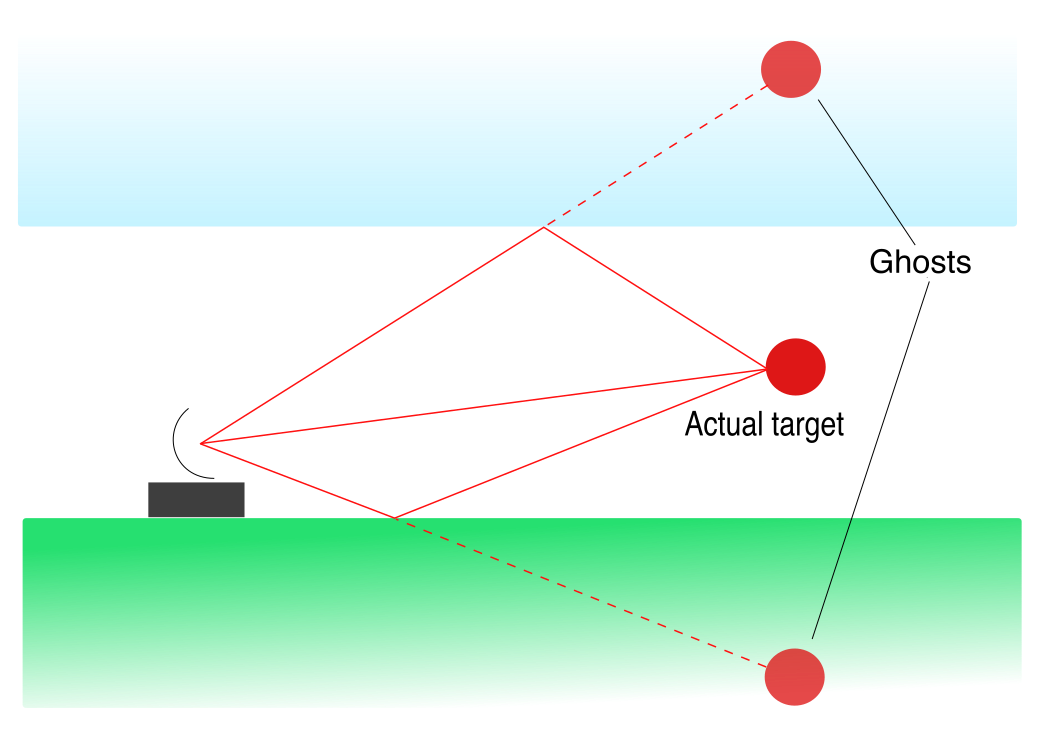
\includegraphics[keepaspectratio]{images/Multipath_propagation_diagram_en.png}}
\caption{Fonte: Wikimedia Commons --- Il trasmettitore invia il segnale
attraverso un percorso diretto e percorsi riflessi dagli edifici,
causando echi.}
\end{figure}

\subsection{Il Problema del Terminale Nascosto (Hidden
Terminal)}\label{il-problema-del-terminale-nascosto-hidden-terminal}

\begin{calloutdefinition}{Terminale Nascosto (Hidden Terminal)}

Si verifica quando due o più stazioni, reciprocamente fuori dal raggio
radio, trasmettono simultaneamente a un destinatario comune, causando
una collisione al ricevitore invisibile ai mittenti.

\end{calloutdefinition}

Se A e C vogliono comunicare con B, ma sono fuori portata tra loro,
entrambi crederanno il canale libero, sovrapponendosi in B.

\begin{figure}
\centering
\pandocbounded{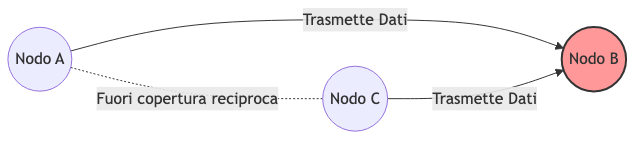
\includegraphics[keepaspectratio,alt={Diagramma del problema del Terminale Nascosto, in cui i nodi A e C non si vedono e trasmettono dati simultaneamente al nodo B, causando in esso una collisione invisibile ai mittenti.}]{images/mermaid-01-fondamenti-wireless-e-protocolli-mac-01.png}}
\caption{Diagramma del problema del Terminale Nascosto, in cui i nodi A
e C non si vedono e trasmettono dati simultaneamente al nodo B, causando
in esso una collisione invisibile ai mittenti.}
\end{figure}

\begin{figure}
\centering
\pandocbounded{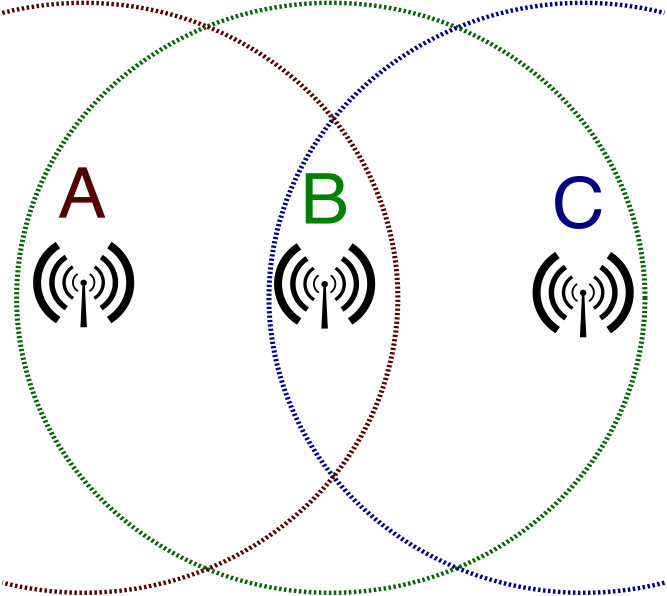
\includegraphics[keepaspectratio]{images/Wifi_hidden_station_problem.png}}
\caption{Fonte: Wikimedia Commons --- I nodi A e C non si trovano nel
reciproco raggio di copertura, ma entrambi raggiungono B.}
\end{figure}

\subsection{Il Problema del Terminale Esposto (Exposed
Terminal)}\label{il-problema-del-terminale-esposto-exposed-terminal}

\begin{calloutdefinition}{Terminale Esposto (Exposed Terminal)}

Una stazione rinuncia inutilmente a trasmettere perché rileva il segnale
di una stazione vicina, pur non essendoci alcun rischio di collisione ai
rispettivi ricevitori.

\end{calloutdefinition}

Se B trasmette ad A, e C desidera trasmettere a D. C ascolta B e,
applicando il CSMA ciecamente, non trasmette per paura di collidere. In
realtà le due comunicazioni potrebbero avvenire in parallelo.

\begin{center}\rule{0.5\linewidth}{0.5pt}\end{center}

\section{4. I Protocolli MAC: Dalle Reti Cablate al
Wireless}\label{i-protocolli-mac-dalle-reti-cablate-al-wireless}

\subsection{I Limiti del CSMA/CD
Cablato}\label{i-limiti-del-csmacd-cablato}

Nelle reti cablate (Ethernet 802.3) il protocollo base è il
\textbf{CSMA/CD} (\emph{Carrier Sense Multiple Access with Collision
Detection}): - \textbf{Carrier Sense}: si ascolta prima di trasmettere.
- \textbf{Collision Detection}: se avviene una collisione in fase di
trasmissione, si interrompe subito l'invio, risparmiando banda. - Per
rilevare collisioni, il frame deve durare almeno il Round Trip Time
(\(2T\)). (Es: a 10 Mbps per \(2T = 51.2\,\mu s\) serve un frame di
almeno 64 byte). - Se avviene collisione, si applica il \textbf{Binary
Exponential Backoff} (attesa casuale in contention slots incrementali).

Nel mondo wireless, non potendo ``ascoltare mentre si parla'' (a causa
del Path Loss) ed essendoci i problemi di terminale nascosto/esposto, il
CSMA/CD è inutilizzabile.

\subsection{I Protocolli MACA e MACAW (Collision
Avoidance)}\label{i-protocolli-maca-e-macaw-collision-avoidance}

Phil Karn (1990) propose il \textbf{MACA} (\emph{Multiple Access with
Collision Avoidance}). Non mira a rilevare collisioni, ma a
\textbf{prevenirle} prenotando il canale.

\subsubsection{Il Meccanismo RTS / CTS}\label{il-meccanismo-rts-cts}

Si basa su un handshake preventivo: 1. \textbf{RTS (Request To Send)}: A
invia a B un pacchetto breve indicando la durata della trasmissione dati
futura. \emph{Le stazioni nel raggio di A lo sentono.} 2. \textbf{CTS
(Clear To Send)}: B risponde con un CTS che conferma la durata. \emph{Le
stazioni nel raggio di B lo sentono.} 3. A riceve il CTS e invia i dati
con sicurezza.

Questa strategia risolve brillantemente le due criticità topologiche: -
\textbf{Gestione dell'Esposto}: Sente l'RTS ma non il CTS. Capisce che
la ricezione avverrà lontano, ed è libero di trasmettere. -
\textbf{Gestione del Nascosto}: Non sente l'RTS ma sente il CTS del
destinatario. Capisce che causerebbe interferenze e si zittisce
disciplinatamente.

Le collisioni possono esserci solo tra RTS piccoli (nessun dato è
perso). In seguito, il protocollo \textbf{MACAW} migliorò il MACA
introducendo il frame di conferma esplicita \textbf{ACK} (vitale nei
canali radio inclini a errori). Queste basi formano il moderno CSMA/CA.

\begin{center}\rule{0.5\linewidth}{0.5pt}\end{center}

\section{5. Lo Standard IEEE 802.11 (Wi-Fi) e
CSMA/CA}\label{lo-standard-ieee-802.11-wi-fi-e-csmaca}

La famiglia \textbf{IEEE 802.11} (Wi-Fi) definisce le WLAN a livello MAC
e Fisico (PHY). Le reti operano tipicamente nelle bande ISM (2.4 GHz) o
U-NII (5, 6 GHz).

\subsection{L'Evoluzione della Famiglia
802.11}\label{levoluzione-della-famiglia-802.11}

\begin{itemize}
\tightlist
\item
  \textbf{802.11 (Legacy)}: (1997) 1-2 Mbps, obsoleto.
\item
  \textbf{802.11a/b/g}: tra il 1999 e 2003, coprono i 2.4 GHz e 5 GHz
  con velocità da 11 a 54 Mbps.
\item
  \textbf{802.11n (WiFi 4)}: (2009) 600 Mbps. Introduce la tecnologia
  \textbf{MIMO} (più antenne in TX/RX).
\item
  \textbf{802.11ac (WiFi 5)}: (2013) 3.47 Gbps massimi sui 5 GHz.
\item
  \textbf{802.11ax (WiFi 6)}: (2020) Fino a 14 Gbps. Ottimizzato per
  alta densità, opera anche a 6 GHz.
\item
  \textbf{802.11af / ah}: varianti a basse frequenze (TV, 900 MHz) per
  lungo raggio/IoT.
\end{itemize}

{\def\LTcaptype{none} % do not increment counter
\begin{longtable}[]{@{}llll@{}}
\toprule\noalign{}
\textbf{Standard} & \textbf{Anno} & \textbf{Max Data Rate} &
\textbf{Frequenza} \\
\midrule\noalign{}
\endhead
\bottomrule\noalign{}
\endlastfoot
\textbf{802.11b/g} & 1999-2003 & 11 - 54 Mbps & 2.4 GHz \\
\textbf{802.11n (WiFi 4)} & 2009 & 600 Mbps & 2.4, 5 GHz \\
\textbf{802.11ac (WiFi 5)} & 2013 & 3.47 Gbps & 5 GHz \\
\textbf{802.11ax (WiFi 6)} & 2020 & 14 Gbps & 2.4, 5, 6 GHz \\
\end{longtable}
}

\subsection{Elementi Architetturali: BSS ed
ESS}\label{elementi-architetturali-bss-ed-ess}

Il blocco logico fondamentale è il \textbf{BSS (Basic Service Set)}. Può
operare come: 1. \textbf{Rete Ad-Hoc}: senza infrastruttura, i nodi sono
peer-to-peer. 2. \textbf{Rete Infrastrutturata}: c'è un \textbf{AP
(Access Point)}. Tutte le comunicazioni passano per l'AP. Più BSS
interconnessi formano un \textbf{ESS (Extended Service Set)} tramite un
Distribution System (DS).

L'associazione host-AP avviene per \textbf{Scansione Passiva} (ascolto
di beacon automatici) o \textbf{Scansione Attiva} (invio di Probe
Request broadcast).

\subsection{Il Sottolivello MAC
802.11}\label{il-sottolivello-mac-802.11}

Il livello MAC è governato da due funzioni: - \textbf{PCF (Point
Coordination Function)}: centralizzato e contention-free (opzionale). -
\textbf{DCF (Distributed Coordination Function)}: obbligatorio e
universale, basato su CSMA/CA distribuito e contention-based.

\subsubsection{Carrier Sensing: Fisico e Virtuale
(NAV)}\label{carrier-sensing-fisico-e-virtuale-nav}

Nel CSMA/CA si usa il Carrier Sensing su due livelli prima di
trasmettere: 1. \textbf{Sensore Fisico}: rileva l'energia
elettromagnetica nel canale. 2. \textbf{Sensore Virtuale (NAV - Network
Allocation Vector)}: timer logico che si basa sulla durata dichiarata
all'interno dei pacchetti altrui (RTS/CTS/Dati). Quando il NAV è attivo,
il canale è considerato virtualmente occupato per tutta la transazione
in corso. Basta che uno dei due sensori dia esito ``occupato'' per
inibire la trasmissione.

\subsubsection{Interframe Spaces (IFS) e
Priorità}\label{interframe-spaces-ifs-e-priorituxe0}

L'accesso al mezzo è regolato da tempi obbligatori di inattività: -
\textbf{DIFS (Distributed IFS)}: tempo di attesa ``lungo'' di default
prima di avviare una trasmissione normale. - \textbf{SIFS (Short IFS)}:
tempo ``brevissimo'', usato esclusivamente prima di messaggi critici
(CTS o ACK). Poiché rigorosamente \textbf{SIFS \textless{} DIFS}, chi ha
appena ricevuto un pacchetto può inviare subito il suo ACK/CTS, rubando
priorità a chiunque altro stia aspettando il termine del DIFS.

\subsubsection{L'Algoritmo CSMA/CA in
Azione}\label{lalgoritmo-csmaca-in-azione}

\begin{enumerate}
\def\labelenumi{\arabic{enumi}.}
\tightlist
\item
  \textbf{Attesa}: Se il canale è ininterrottamente libero per un DIFS,
  l'host trasmette.
\item
  \textbf{Backoff}: Se è occupato, fa partire un timer casuale di
  backoff. Il timer decresce \emph{solo} se il canale è libero; si
  congela se occupato. Quando arriva a zero (e trascorre un DIFS),
  trasmette.
\item
  \textbf{ACK}: Se i dati arrivano a destinazione intatti, il ricevitore
  aspetta un SIFS e risponde con un \textbf{ACK}.
\item
  \textbf{Collisione/Fallimento}: Se l'ACK non giunge, il mittente
  deduce il fallimento, innesca la penalità raddoppiando l'intervallo di
  backoff (Binary Exponential Backoff) e riprova l'invio.
\end{enumerate}

\subsubsection{RTS/CTS nel DCF}\label{rtscts-nel-dcf}

Il meccanismo RTS/CTS è un'opzione preziosa per evitare spreco di enormi
pacchetti Dati (soggetti a collisioni). La sua attivazione (RTS
Threshold) può essere impostata su \emph{Mai} (traffico scarso),
\emph{Soglia} (solo per grandi payload) o \emph{Sempre} (alta
congestione/nodi nascosti).

\begin{center}\rule{0.5\linewidth}{0.5pt}\end{center}

\begin{calloutquestion}{Possibili domande d’esame}

- Qual è la differenza tra rete single-hop e multi-hop con
infrastruttura? - Perché il CSMA/CD non può essere applicato nelle reti
wireless? Quale protocollo lo sostituisce e con quale logica? - Definire
la Shannon Capacity e spiegare perché la capacità scala logaritmicamente
con l'SNR e non linearmente. - Descrivere il problema del terminale
nascosto ed esposto e come il meccanismo RTS/CTS li risolve. - Cosa si
intende per Multipath e Coherence Time? - Come operano il Carrier
Sensing Virtuale e il NAV? - Perché è essenziale che il tempo SIFS sia
minore del DIFS? - Qual è il ruolo dell'ACK e del Backoff Esponenziale
in CSMA/CA?

\end{calloutquestion}

\newpage

\chapter{02 - Teoria dei Segnali: Introduzione, Fourier, Campionamento e
DFT}\label{teoria-dei-segnali-introduzione-fourier-campionamento-e-dft}

\section{Perché la Teoria dei
Segnali?}\label{perchuxe9-la-teoria-dei-segnali}

I sistemi moderni --- reti mobili 4G/5G, dispositivi IoT, sistemi audio
--- elaborano \textbf{segnali} per rappresentare e trasmettere
informazione. Capire come questi segnali sono strutturati, come vengono
disturbati dal canale trasmissivo, e come possono essere analizzati e
trasformati è il fondamento dell'ingegneria delle comunicazioni
digitali.

La teoria dei segnali serve a quattro scopi pratici fondamentali. Il
primo è \textbf{estrarre informazione}: identificare frequenze, pattern
ed eventi rilevanti (es. riconoscimento vocale, analisi di segnali
biomedici). Il secondo è \textbf{rimuovere effetti indesiderati}:
filtrare il rumore, compensare distorsioni del canale, mitigare il
fading multipath nelle reti wireless. Il terzo è \textbf{trasmettere
efficientemente l'informazione}: codificare i segnali per il canale (es.
OFDM in 4G/5G che distribuisce i dati su più frequenze). Il quarto è
\textbf{abilitare l'elaborazione digitale}: convertire segnali analogici
in forma digitale tramite campionamento e quantizzazione.

\begin{figure}
\centering
\pandocbounded{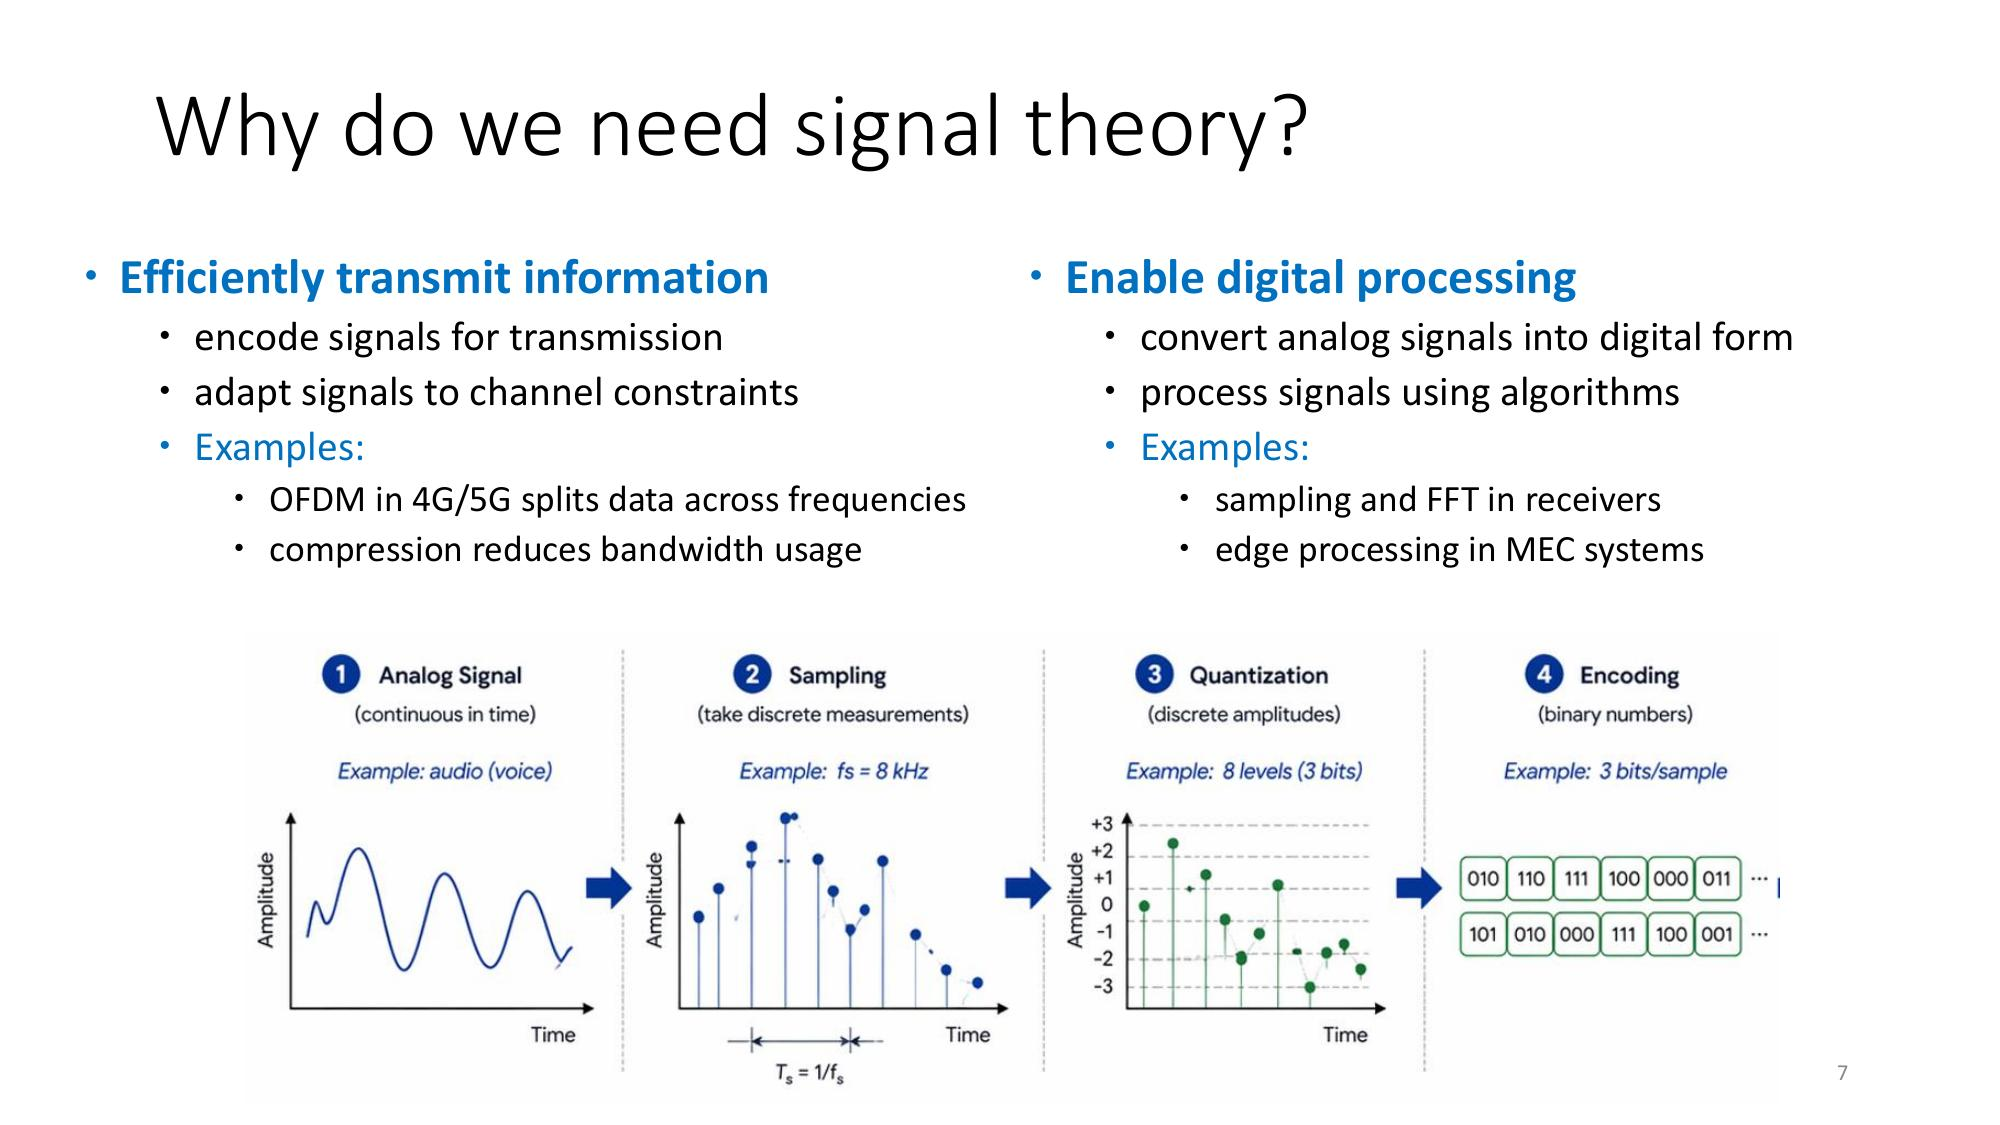
\includegraphics[keepaspectratio]{images/lezione-25-lab-teoria-dei-segnali-introduzione-e-serie-di-fourier-img-01.jpg}}
\caption{Dalla sorgente analogica ai bit: campionamento
(discretizzazione nel tempo), quantizzazione (discretizzazione
dell'ampiezza), codifica binaria.}
\end{figure}

\begin{center}\rule{0.5\linewidth}{0.5pt}\end{center}

\section{Classificazione dei Segnali}\label{classificazione-dei-segnali}

\begin{calloutdefinition}{Segnale}

Un segnale è una variazione di una grandezza fisica che porta
informazione. Formalmente è una funzione
\(f(t): \mathfrak{D} \longrightarrow \mathfrak{C}\) dove il dominio
\(\mathfrak{D}\) può essere \(\mathbb{R}\) (tempo continuo) o
\(\mathbb{Z}\) (tempo discreto), e il codominio \(\mathfrak{C}\) può
essere \(\mathbb{R}\) (ampiezza continua) o un insieme discreto
(ampiezza quantizzata).

\end{calloutdefinition}

Ci concentriamo su \textbf{segnali deterministici monodimensionali}: la
variabile indipendente è il tempo, e il segnale è noto prima di essere
prodotto (al contrario dei segnali aleatori, analizzati con metodi
probabilistici).

\subsection{Segnali a Tempo Continuo}\label{segnali-a-tempo-continuo}

Quando il dominio è \(\mathbb{R}\), il segnale è detto
\textbf{analogico} (\emph{analog}). Se anche il codominio è
\(\mathbb{R}\), l'ampiezza è continua; se il codominio è un insieme
discreto (es. \(\mathbb{Z}\)), l'ampiezza è quantizzata.

\begin{figure}
\centering
\pandocbounded{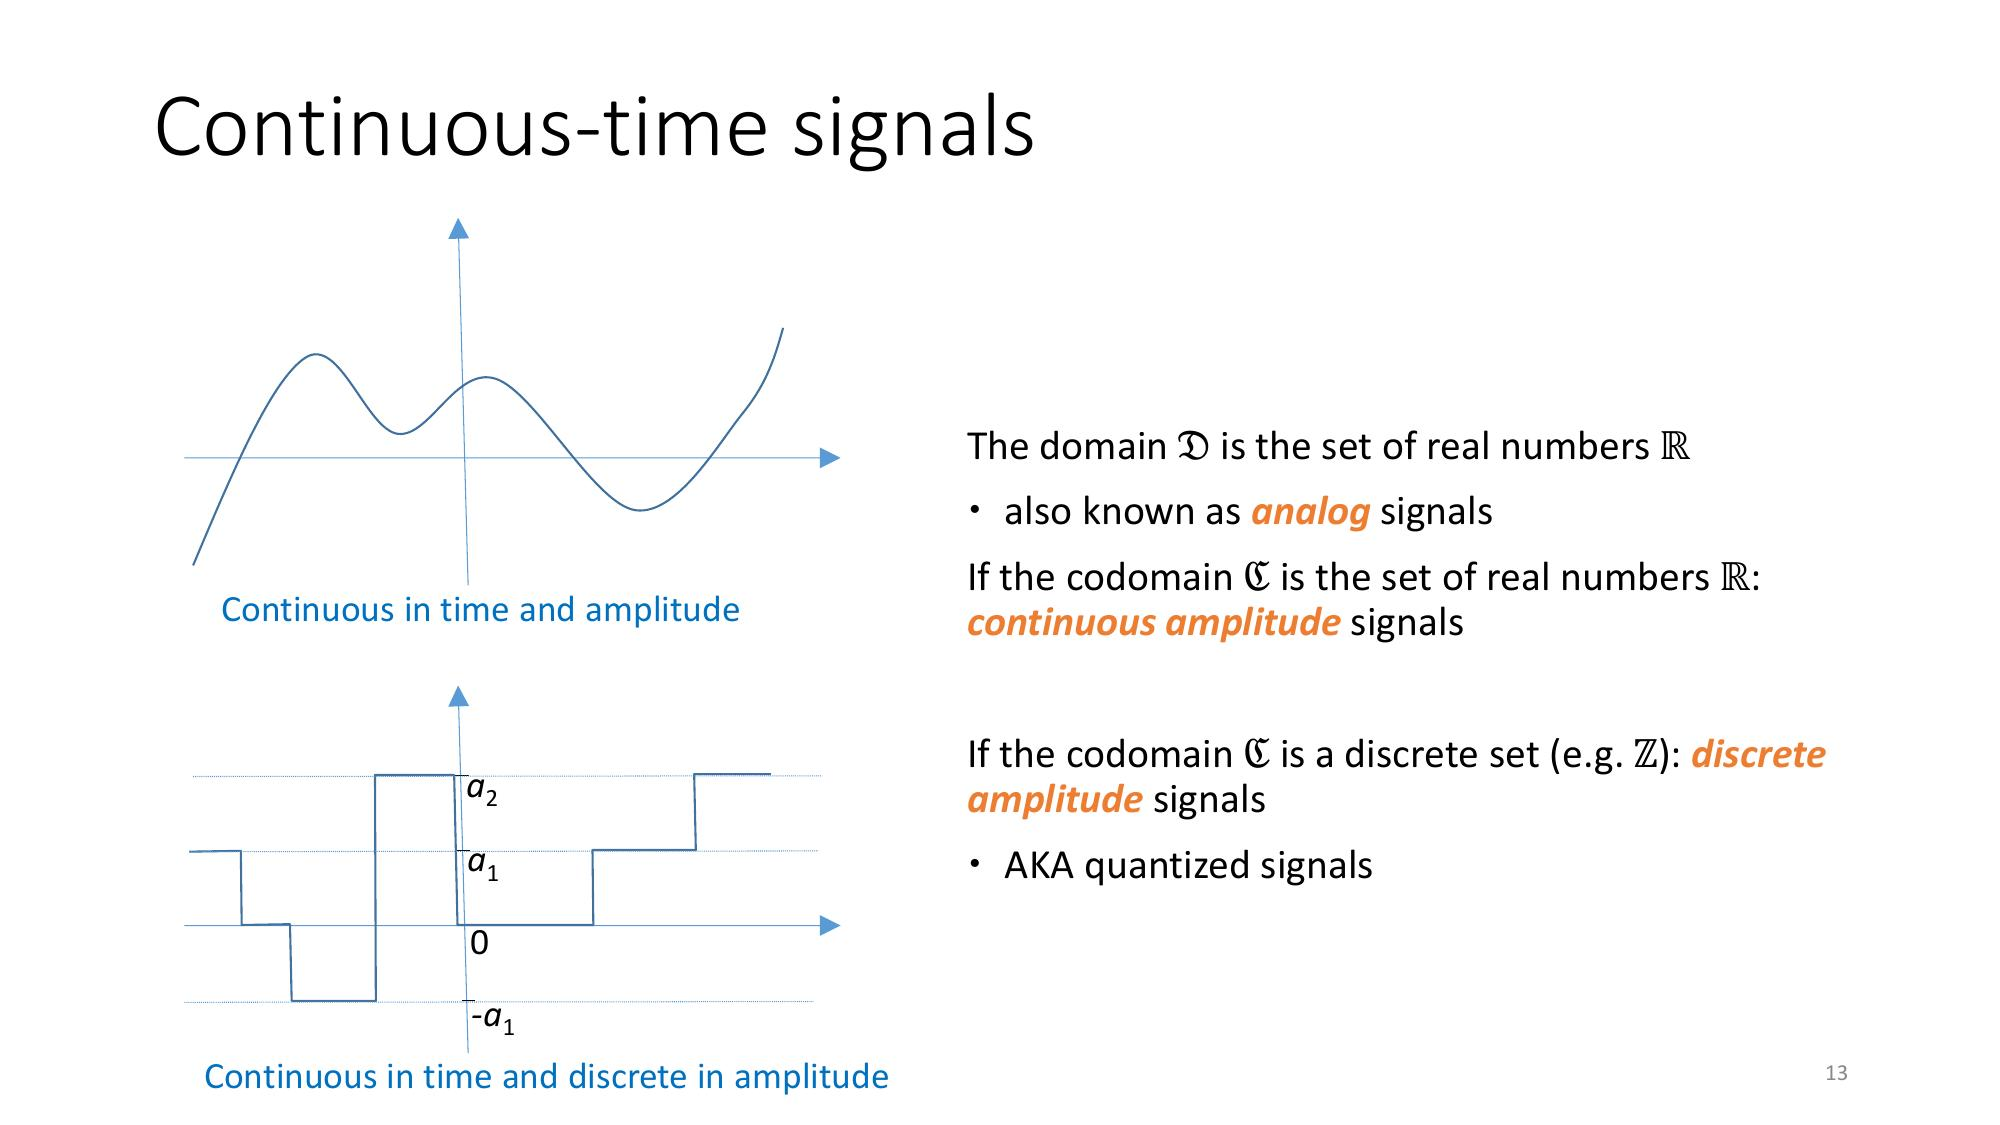
\includegraphics[keepaspectratio]{images/lezione-25-lab-teoria-dei-segnali-introduzione-e-serie-di-fourier-img-02.jpg}}
\caption{In alto: segnale analogico, continuo in tempo e ampiezza. In
basso: segnale continuo in tempo ma quantizzato in ampiezza (segnale a
gradini).}
\end{figure}

\subsection{Segnali a Tempo Discreto}\label{segnali-a-tempo-discreto}

Quando il dominio è
\(\mathbb{Z}(T) = \{nT, \forall n \in \mathbb{Z}, T \in \mathbb{R}\}\),
il segnale è detto \textbf{discreto}. Ad esempio
\(\mathbb{Z}(2) = \{\ldots, -4, -2, 0, 2, 4, \ldots\}\). Un segnale
discreto con ampiezza presa da un insieme finito di simboli è detto
\textbf{digitale} (\emph{digital}), o sequenza simbolica.

\begin{figure}
\centering
\pandocbounded{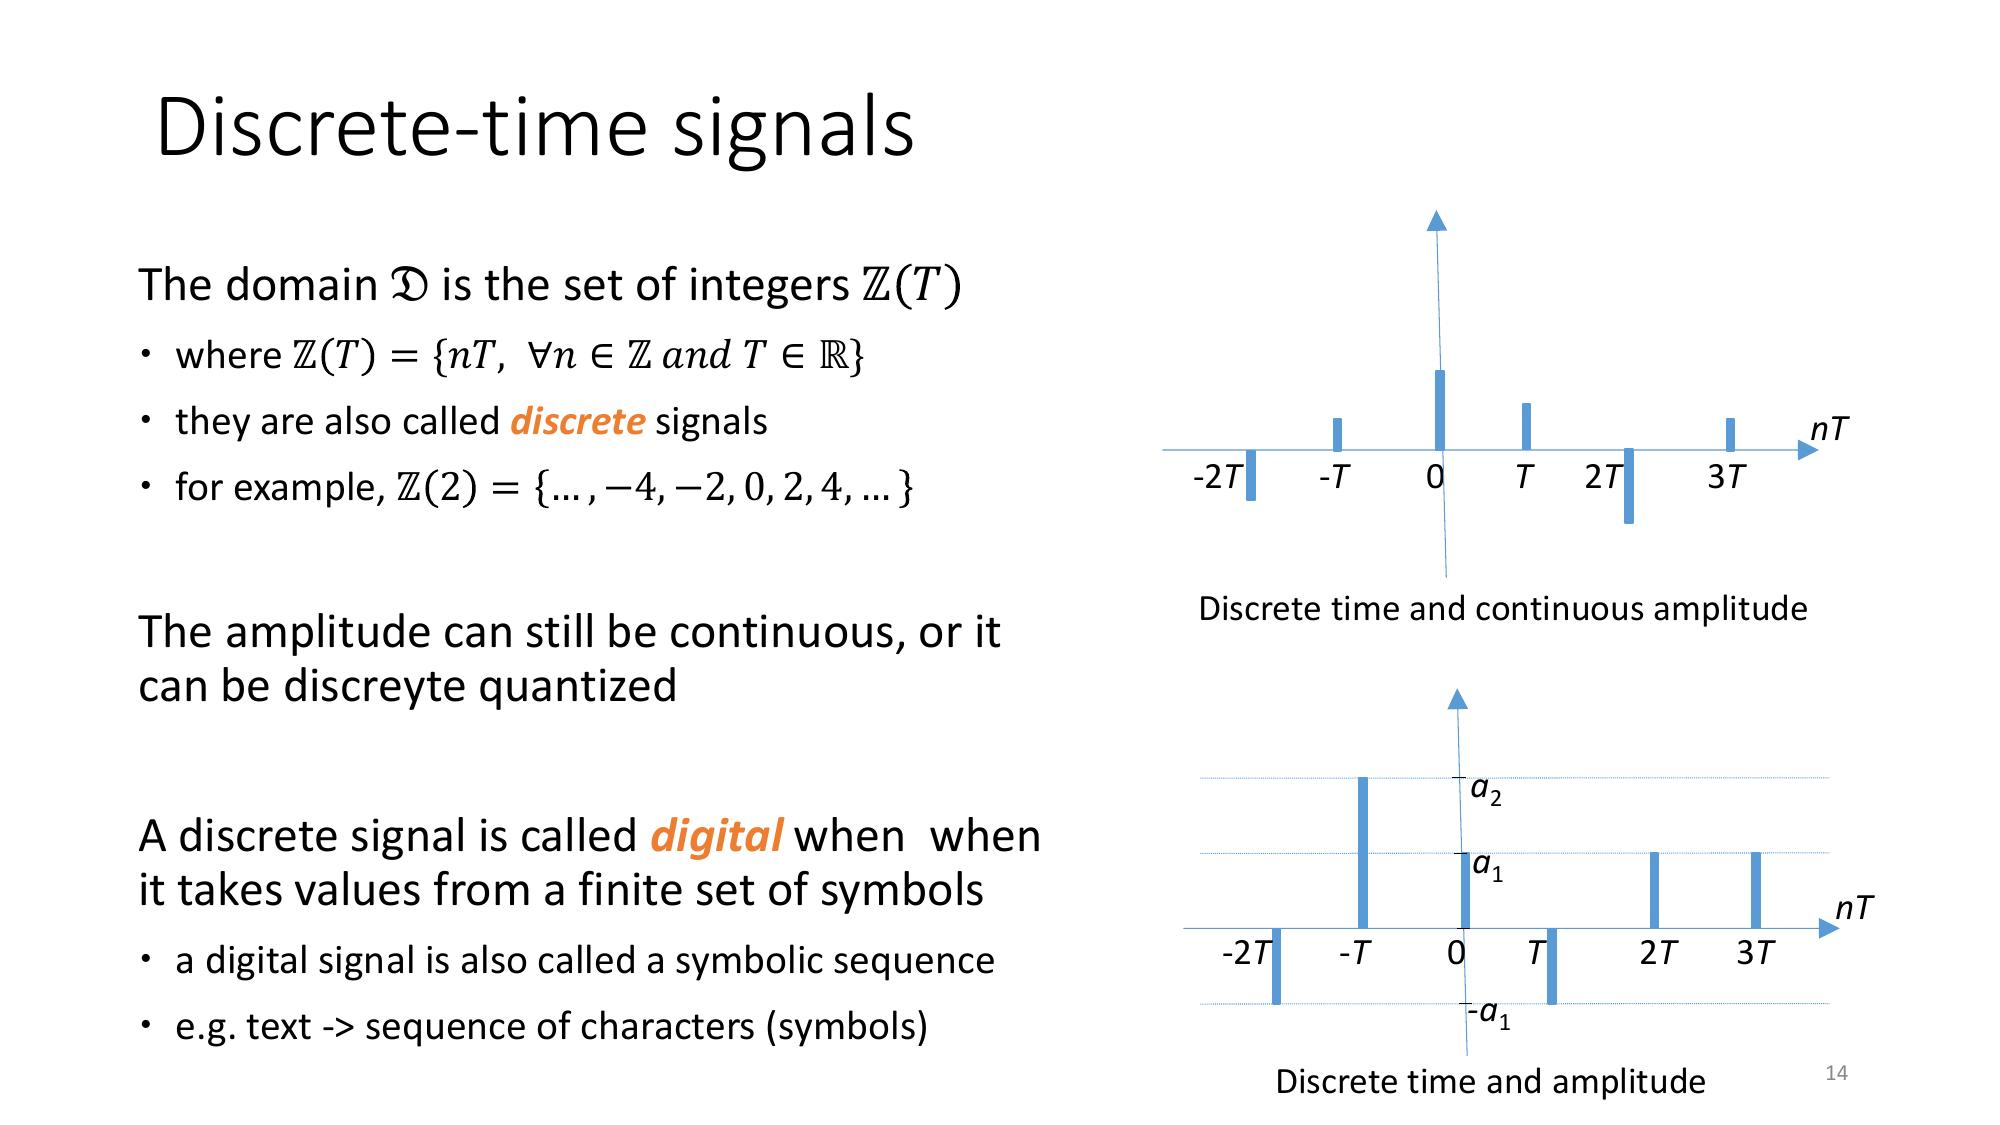
\includegraphics[keepaspectratio]{images/lezione-25-lab-teoria-dei-segnali-introduzione-e-serie-di-fourier-img-03.jpg}}
\caption{In alto: segnale discreto con ampiezza continua. In basso:
segnale digitale, discreto sia nel tempo che nell'ampiezza.}
\end{figure}

\subsection{Tabella Riepilogativa}\label{tabella-riepilogativa}

{\def\LTcaptype{none} % do not increment counter
\begin{longtable}[]{@{}
  >{\raggedright\arraybackslash}p{(\linewidth - 4\tabcolsep) * \real{0.3333}}
  >{\raggedright\arraybackslash}p{(\linewidth - 4\tabcolsep) * \real{0.3333}}
  >{\raggedright\arraybackslash}p{(\linewidth - 4\tabcolsep) * \real{0.3333}}@{}}
\toprule\noalign{}
\begin{minipage}[b]{\linewidth}\raggedright
Tempo
\end{minipage} & \begin{minipage}[b]{\linewidth}\raggedright
Ampiezza
\end{minipage} & \begin{minipage}[b]{\linewidth}\raggedright
Tipo
\end{minipage} \\
\midrule\noalign{}
\endhead
\bottomrule\noalign{}
\endlastfoot
Continuo (\(\mathbb{R}\)) & Continua (\(\mathbb{R}\)) & Segnale
analogico \\
Continuo (\(\mathbb{R}\)) & Discreta (\(\mathbb{Z}\)) & Segnale
quantizzato \\
Discreto (\(\mathbb{Z}(T)\)) & Continua (\(\mathbb{R}\)) & Segnale
discreto \\
Discreto (\(\mathbb{Z}(T)\)) & Discreta (insieme finito) & Segnale
digitale \\
\end{longtable}
}

\subsection{Bitrate di una Sorgente
Digitale}\label{bitrate-di-una-sorgente-digitale}

Quando un segnale analogico viene convertito in digitale con frequenza
di campionamento \(f_c\) campioni/secondo e ogni campione è codificato
con \(M\) bit:

\[\text{Bitrate} = f_c \cdot M \quad [\text{bit/secondo}]\]

Maggiori \(f_c\) e \(M\) producono migliore fedeltà ma richiedono
maggiore capacità trasmissiva.

\begin{center}\rule{0.5\linewidth}{0.5pt}\end{center}

\section{Trasmissione e Canale}\label{trasmissione-e-canale}

\subsection{Il Modello del Canale}\label{il-modello-del-canale}

Nella trasmissione di informazione, un trasduttore alla sorgente
converte un messaggio in un segnale fisico (es. un'antenna converte
energia elettrica in onde elettromagnetiche), il segnale si propaga
attraverso il mezzo, e un trasduttore alla destinazione converte il
segnale di ritorno in messaggio. Il \textbf{canale} non è un mezzo
ideale: agisce come un sistema che modifica il segnale.

Le principali forme di degrado sono la \textbf{distorsione} (variazione
della forma d'onda, es. attenuazione differenziata per frequenza), la
\textbf{propagazione multipath} (il segnale raggiunge il ricevitore
attraverso percorsi multipli con ritardi diversi, causando
interferenza), e il \textbf{rumore} (segnale indesiderato sovrapposto a
quello utile).

\begin{calloutdefinition}{SNR — Signal-to-Noise Ratio}

Il rapporto segnale-rumore misura la qualità del segnale ricevuto
rispetto al rumore di fondo:
\[SNR_{dB} = 10 \log_{10} \frac{P_{signal}}{P_{noise}}\]

\end{calloutdefinition}

\subsection{Teorema di Shannon}\label{teorema-di-shannon}

Il risultato fondamentale della teoria dell'informazione stabilisce la
capacità massima di un canale:

\[C = B \log_2 (1 + SNR)\]

dove \(B\) è la banda disponibile in Hz, \(SNR\) il rapporto
segnale-rumore, e \(C\) la capacità del canale in bit/secondo. Questo
crea un trade-off inevitabile: ridurre la distorsione di quantizzazione
alla sorgente aumenta la quantità di informazione da trasmettere, che
deve rientrare entro la capacità \(C\).

\begin{center}\rule{0.5\linewidth}{0.5pt}\end{center}

\section{Serie di Fourier: dal Tempo alla
Frequenza}\label{serie-di-fourier-dal-tempo-alla-frequenza}

\subsection{L'Intuizione Fondamentale}\label{lintuizione-fondamentale}

Un segnale periodico può essere visto come una sovrapposizione di
componenti sinusoidali, ciascuna con frequenza, ampiezza e fase
specifiche. Questo cambio di prospettiva --- dal dominio del tempo al
\textbf{dominio della frequenza} --- è cruciale perché il canale
trasmissivo agisce in modo diverso su componenti a frequenza diversa.
Per analizzare e predire tale comportamento, occorre identificare
esplicitamente le componenti frequenziali di un segnale.

La serie di Fourier decompone una funzione come somma di infinite
funzioni oscillanti a frequenze diverse. È formalmente un cambio di
coordinate: dal dominio del tempo a quello della frequenza. La base di
questa decomposizione è un insieme di funzioni \(\varphi_n(t)\)
ortogonali, analogamente alla decomposizione di un vettore in uno spazio
vettoriale.

\begin{figure}
\centering
\pandocbounded{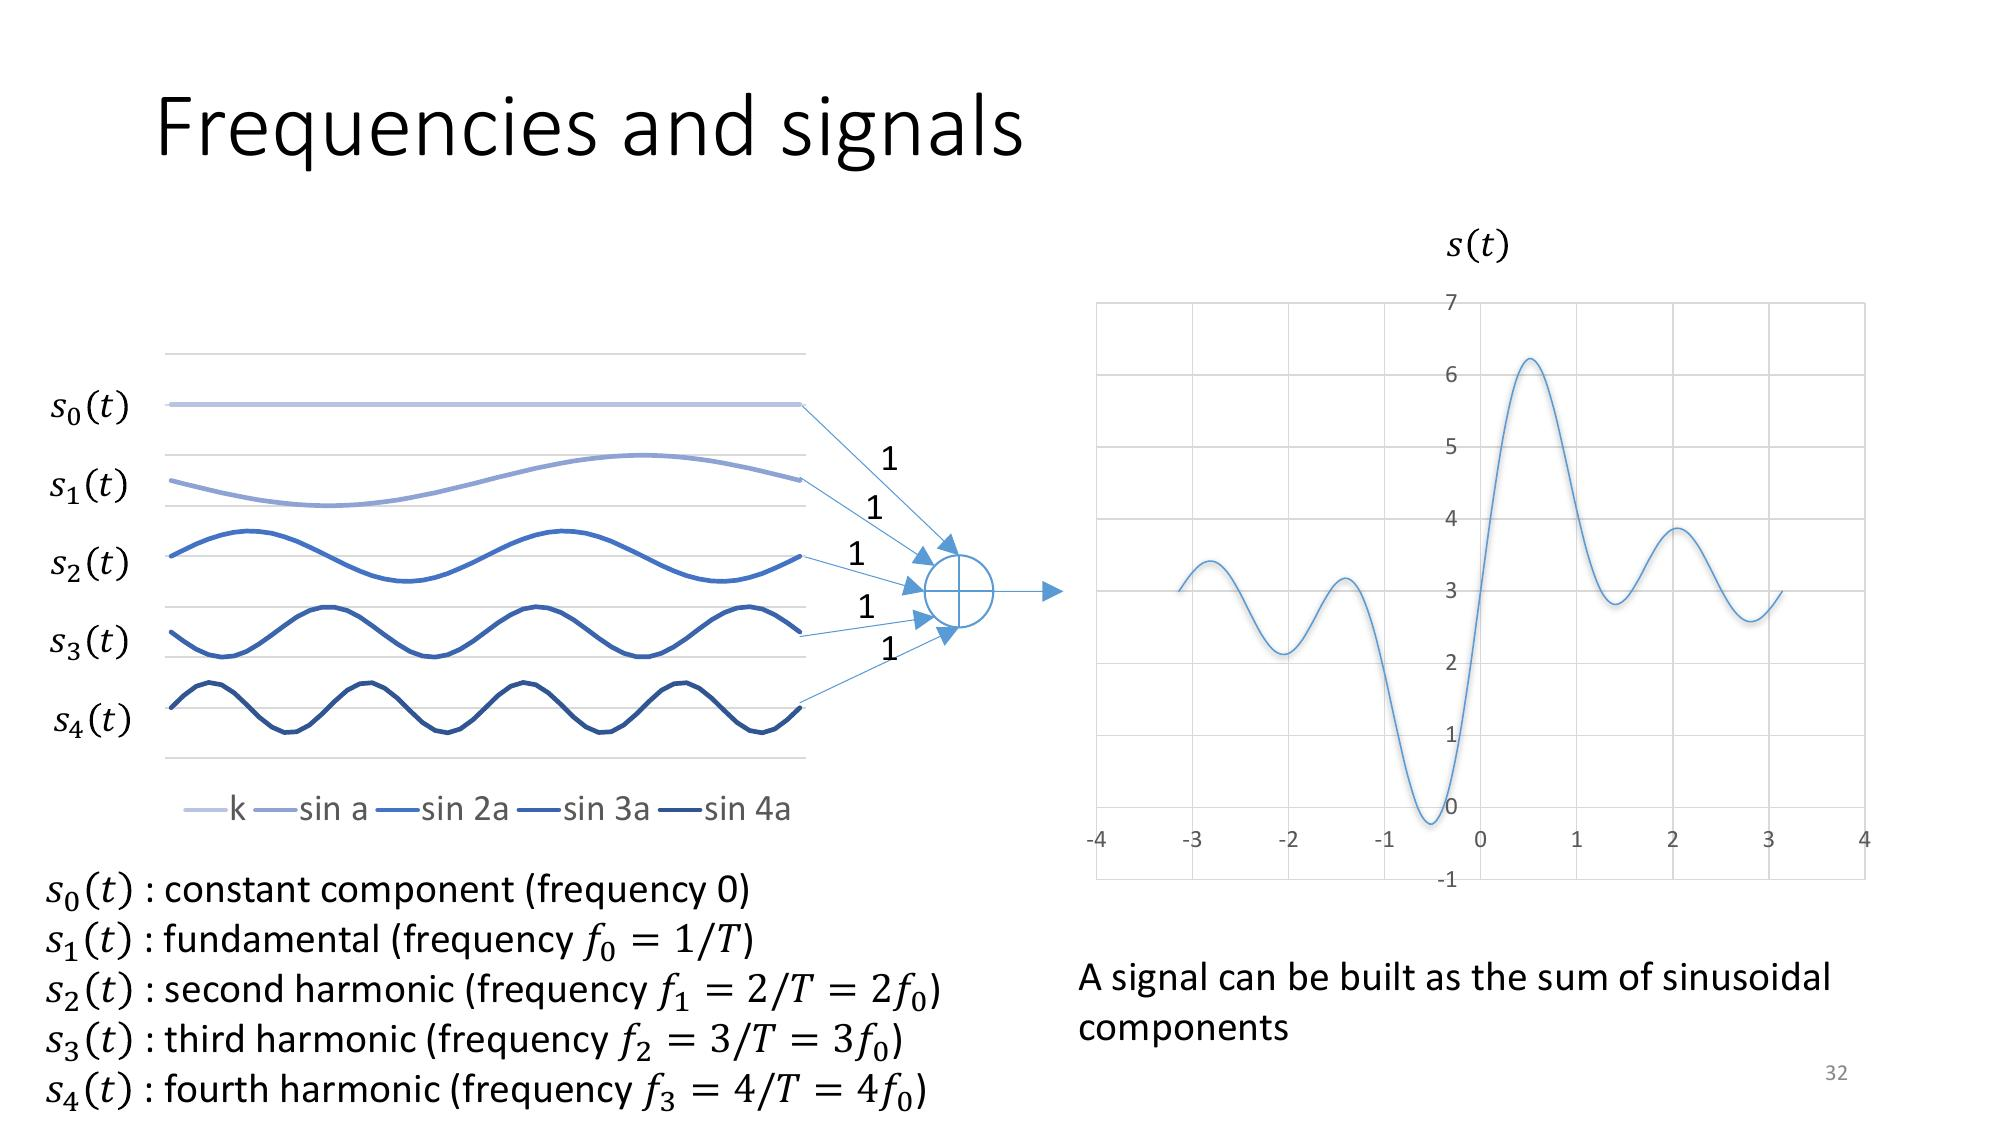
\includegraphics[keepaspectratio]{images/lezione-25-lab-teoria-dei-segnali-introduzione-e-serie-di-fourier-img-04.jpg}}
\caption{Un segnale si costruisce sommando componenti sinusoidali: la
componente costante (\(s_0\)), la fondamentale (\(s_1\)) e le armoniche
superiori (\(s_2, s_3, s_4\)). Cambiare i coefficienti cambia il segnale
risultante.}
\end{figure}

\subsection{Segnali Periodici
Continui}\label{segnali-periodici-continui}

Un segnale continuo \(s(t): \mathbb{R} \to \mathbb{R}\) è
\textbf{periodico con periodo \(T\)} se

\[s(t) = s(t + T) \quad \forall t \in \mathbb{R}\]

I segnali periodici si possono studiare interamente nell'intervallo
\([0, T]\). La frequenza fondamentale è \(f = 1/T\). Un segnale non
periodico è detto \textbf{aperiodico}.

\subsection{Definizione della Serie di
Fourier}\label{definizione-della-serie-di-fourier}

\begin{calloutdefinition}{Serie di Fourier (intervallo [-\\pi, \\pi])}

Data una funzione continua \(s(t): \mathbb{R} \to \mathbb{R}\) periodica
in \([-\pi, \pi]\):
\[s(t) = \frac{1}{2} a_0 + \sum_{n=1}^{\infty} \left( a_n \cos(nt) + b_n \sin(nt) \right)\]
con coefficienti:
\[a_0 = \frac{1}{\pi} \int_{-\pi}^{\pi} s(t)\, dt \qquad a_n = \frac{1}{\pi} \int_{-\pi}^{\pi} s(t) \cos(nt)\, dt \qquad b_n = \frac{1}{\pi} \int_{-\pi}^{\pi} s(t) \sin(nt)\, dt\]

\end{calloutdefinition}

Il termine \(\frac{1}{2} a_0\) è la \textbf{componente continua} (media
del segnale); i termini \(a_n \cos(nt) + b_n \sin(nt)\) sono le
\textbf{armoniche} di frequenza \(n/T\).

\subsection{Condizioni di Dirichlet}\label{condizioni-di-dirichlet}

La serie di Fourier non è definita per qualsiasi funzione. Non sono note
le condizioni necessarie, ma esistono condizioni \textbf{sufficienti}
(teorema di Dirichlet):

\begin{callouttheorem}{Teorema di Dirichlet}

Se \(s(t)\) è periodica e \textbf{piecewise continuous} (composta da un
numero finito di pezzi continui su ogni sottointervallo finito, con
limite finito nei punti di discontinuità), allora la serie di Fourier di
\(s(t)\) esiste e converge in \(\mathbb{R}\).

\end{callouttheorem}

\subsection{Esempio: Onda Quadra}\label{esempio-onda-quadra}

Consideriamo il segnale periodico con periodo \(2\pi\):

\[s(t) = \begin{cases} 2 & \text{se } -\pi < t < 0 \\ 1 & \text{se } 0 \le t \le \pi \end{cases}\]

Il calcolo dei coefficienti porta a:

\[a_0 = 3, \qquad a_n = 0, \qquad b_n = \begin{cases} 0 & \text{se } n \text{ pari} \\ -\frac{2}{n\pi} & \text{se } n \text{ dispari} \end{cases}\]

La serie risultante, ponendo \(n = 2k-1\), è:

\[s(t) = \frac{3}{2} - \sum_{k=1}^{\infty} \frac{2}{(2k-1)\pi} \sin\bigl((2k-1)t\bigr)\]

Solo le armoniche \textbf{dispari} contribuiscono, e la loro ampiezza
cala come \(1/n\).

\subsection{Fenomeno di Gibbs}\label{fenomeno-di-gibbs}

Quando la serie di Fourier approssima una funzione con discontinuità
(come un'onda quadra), si osserva un \textbf{overshoot} intorno ai punti
di salto che non scompare mai, per quanto si aumenti il numero di
armoniche. Questo è il \textbf{fenomeno di Gibbs}: la serie converge in
senso \(L^2\), ma nelle vicinanze di ogni discontinuità l'errore rimane
del \textasciitilde9\% del salto, indipendentemente dall'ordine di
troncamento.

\begin{figure}
\centering
\pandocbounded{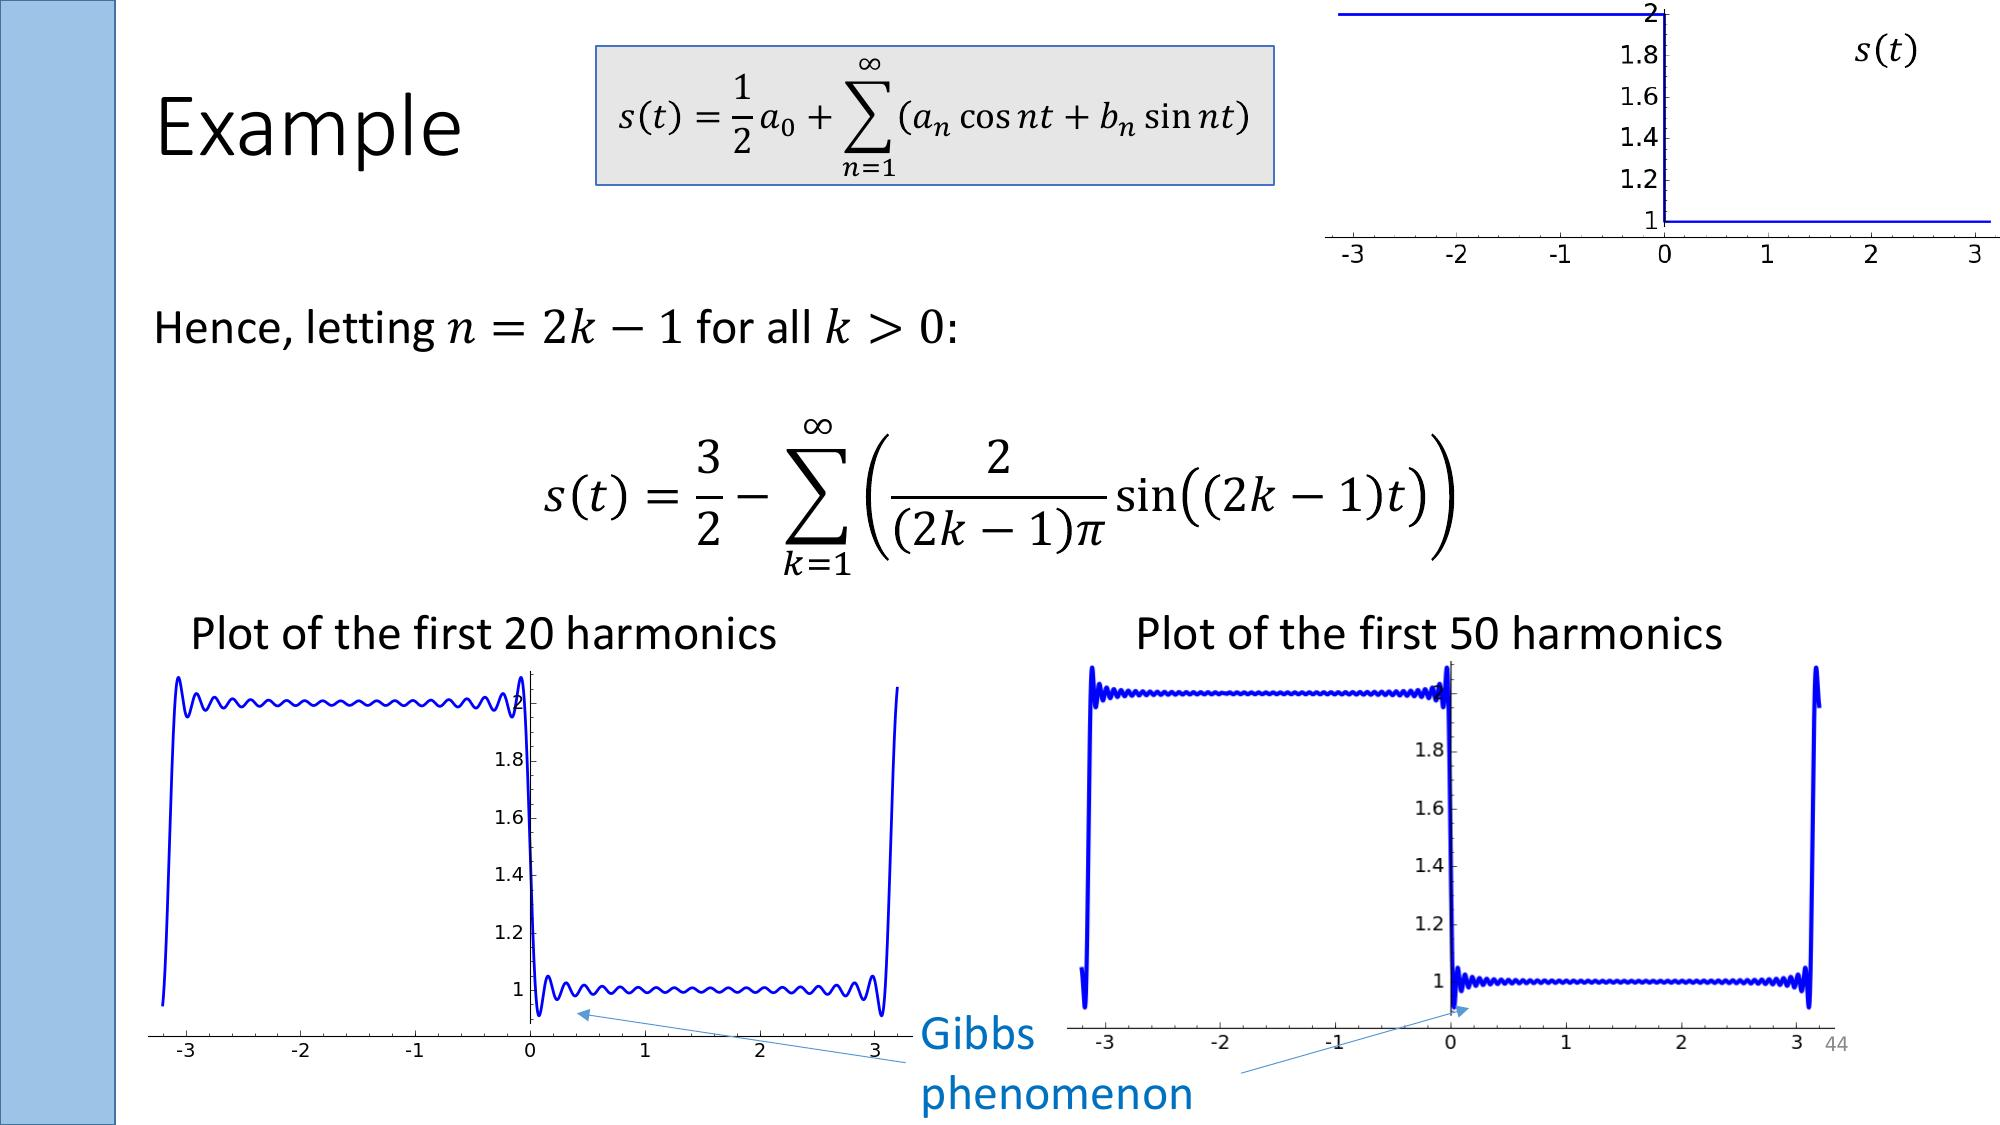
\includegraphics[keepaspectratio]{images/lezione-25-lab-teoria-dei-segnali-introduzione-e-serie-di-fourier-img-05.jpg}}
\caption{Fenomeno di Gibbs: aggiungere più armoniche riduce le
oscillazioni nel tratto piatto, ma l'overshoot al salto rimane costante
(\textasciitilde9\% del salto).}
\end{figure}

\begin{center}\rule{0.5\linewidth}{0.5pt}\end{center}

\section{Serie di Fourier con Periodo
Arbitrario}\label{serie-di-fourier-con-periodo-arbitrario}

La definizione si estende naturalmente a segnali con periodo generico
\(T\). Tramite la sostituzione \(y = 2\pi t / T\), un segnale periodico
in \([-T/2, T/2]\) si trasforma in uno periodico in \([-\pi, \pi]\), e i
coefficienti diventano:

\[s(t) = \frac{1}{2} a_0 + \sum_{n=1}^{\infty} \left( a_n \cos\frac{2\pi n t}{T} + b_n \sin\frac{2\pi n t}{T} \right)\]

con

\[a_0 = \frac{2}{T} \int_{-T/2}^{T/2} s(t)\, dt \qquad a_n = \frac{2}{T} \int_{-T/2}^{T/2} s(t) \cos\frac{2\pi n t}{T}\, dt \qquad b_n = \frac{2}{T} \int_{-T/2}^{T/2} s(t) \sin\frac{2\pi n t}{T}\, dt\]

\begin{center}\rule{0.5\linewidth}{0.5pt}\end{center}

\section{Numeri Complessi e Formula di
Eulero}\label{numeri-complessi-e-formula-di-eulero}

Prima di passare alla forma esponenziale della serie, è necessario
richiamare i \textbf{numeri complessi}. Un numero complesso
\(\bar{x} = a + jb\) ha parte reale \(a\) e parte immaginaria \(b\) (con
\(j = \sqrt{-1}\)). Nel piano complesso è rappresentato come un vettore
di modulo \(|\bar{x}| = \sqrt{a^2 + b^2}\) e fase
\(\varphi = \tan^{-1}(b/a)\).

\begin{calloutdefinition}{Formula di Eulero}

\[e^{\pm j\varphi} = \cos\varphi \pm j\sin\varphi\]

Da cui si derivano le formule inverse:
\[\cos\varphi = \frac{e^{j\varphi} + e^{-j\varphi}}{2} \qquad \sin\varphi = \frac{e^{j\varphi} - e^{-j\varphi}}{2j}\]

\end{calloutdefinition}

Usando l'esponenziale di Eulero, ogni numero complesso si scrive
compattamente come \(\bar{x} = |x| e^{j\varphi}\), che combina modulo e
fase in un unico termine. Questo è particolarmente potente per
rappresentare segnali: ampiezza e fase di ogni armonica vengono
codificate in un unico coefficiente complesso.

\begin{center}\rule{0.5\linewidth}{0.5pt}\end{center}

\section{Serie di Fourier in Forma
Esponenziale}\label{serie-di-fourier-in-forma-esponenziale}

\subsection{La Base Esponenziale}\label{la-base-esponenziale}

La serie di Fourier generalizzata al dominio complesso usa come base
l'insieme di funzioni:

\[e^{j2\pi n F t} \quad \forall n \in \mathbb{Z}\]

poiché \(e^{j2\pi n F t} = \cos(2\pi n F t) + j\sin(2\pi n F t)\), ogni
elemento della base è una sinusoide complessa alla frequenza \(nF\).

\begin{calloutdefinition}{Serie di Fourier esponenziale}

Dato un segnale periodico \(s(t) = s(t+T)\) con frequenza fondamentale
\(F = 1/T\):
\[s(t) = \sum_{n=-\infty}^{+\infty} S_n \, e^{j2\pi n F t}\]

dove i coefficienti \(S_n\) (in generale complessi) si calcolano come:
\[S_n = \frac{1}{T} \int_{0}^{T} s(t) \, e^{-j2\pi n F t}\, dt\]

\end{calloutdefinition}

I coefficienti \(S_n\) codificano sia ampiezza che fase di ogni
armonica: \(S_n = |S_n| e^{j\phi_n}\), dove \(|S_n|\) è l'ampiezza e
\(\phi_n = \arg(S_n)\) è la fase dell'armonica \(n\)-esima.

\subsection{Interpretazione
Geometrica}\label{interpretazione-geometrica}

Per \(n = 0\): la componente continua (media del segnale),
\(S_0 = \frac{1}{T}\int_0^T s(t)\, dt\).\\
Per \(n = \pm 1\): frequenza fondamentale \(F\), periodo \(T\).\\
Per \(|n| > 1\): armoniche di frequenza \(nF\), periodo \(T/n\).

\begin{callouttip}{Perché la forma complessa?}

Con i numeri reali occorrono due coefficienti (\(a_n\) e \(b_n\)) per
descrivere ogni armonica. Con la forma complessa basta un solo
coefficiente \(S_n\) che ne racchiude entrambi. Questo semplifica
enormemente la manipolazione matematica e consente di rappresentare
segnali \(s(t): \mathbb{R} \to \mathbb{C}\), generalizzando la serie per
funzioni reali.

\end{callouttip}

\subsection{Esempio: Onda Rettangolare con Base
Esponenziale}\label{esempio-onda-rettangolare-con-base-esponenziale}

Consideriamo il segnale di periodo \(T\) e frequenza \(F = 1/T\):

\[s(t) = \begin{cases} 1 & \text{se } |t| \le T/4 \\ 0 & \text{se } T/4 < |t| \le T/2 \end{cases}\]

Il calcolo dei coefficienti dà:

\[S_n = \begin{cases} 1/2 & n = 0 \\ 0 & n \text{ pari} \\ \dfrac{(-1)^k}{-(2k-1)\pi} & n = 2k-1 \end{cases}\]

La serie risultante è quindi:

\[s(t) = \frac{1}{2} + \sum_{k=-\infty}^{+\infty} -\frac{(-1)^k}{(2k-1)\pi} \cos\bigl(2\pi(2k-1)Ft\bigr)\]

Il grafico seguente mostra la convergenza della serie per \(T=4\) con
\(k \in [-1,1]\) (verde), \(k \in [-2,2]\) (rosso) e
\(k \in [-100,100]\) (blu):

\begin{figure}
\centering
\pandocbounded{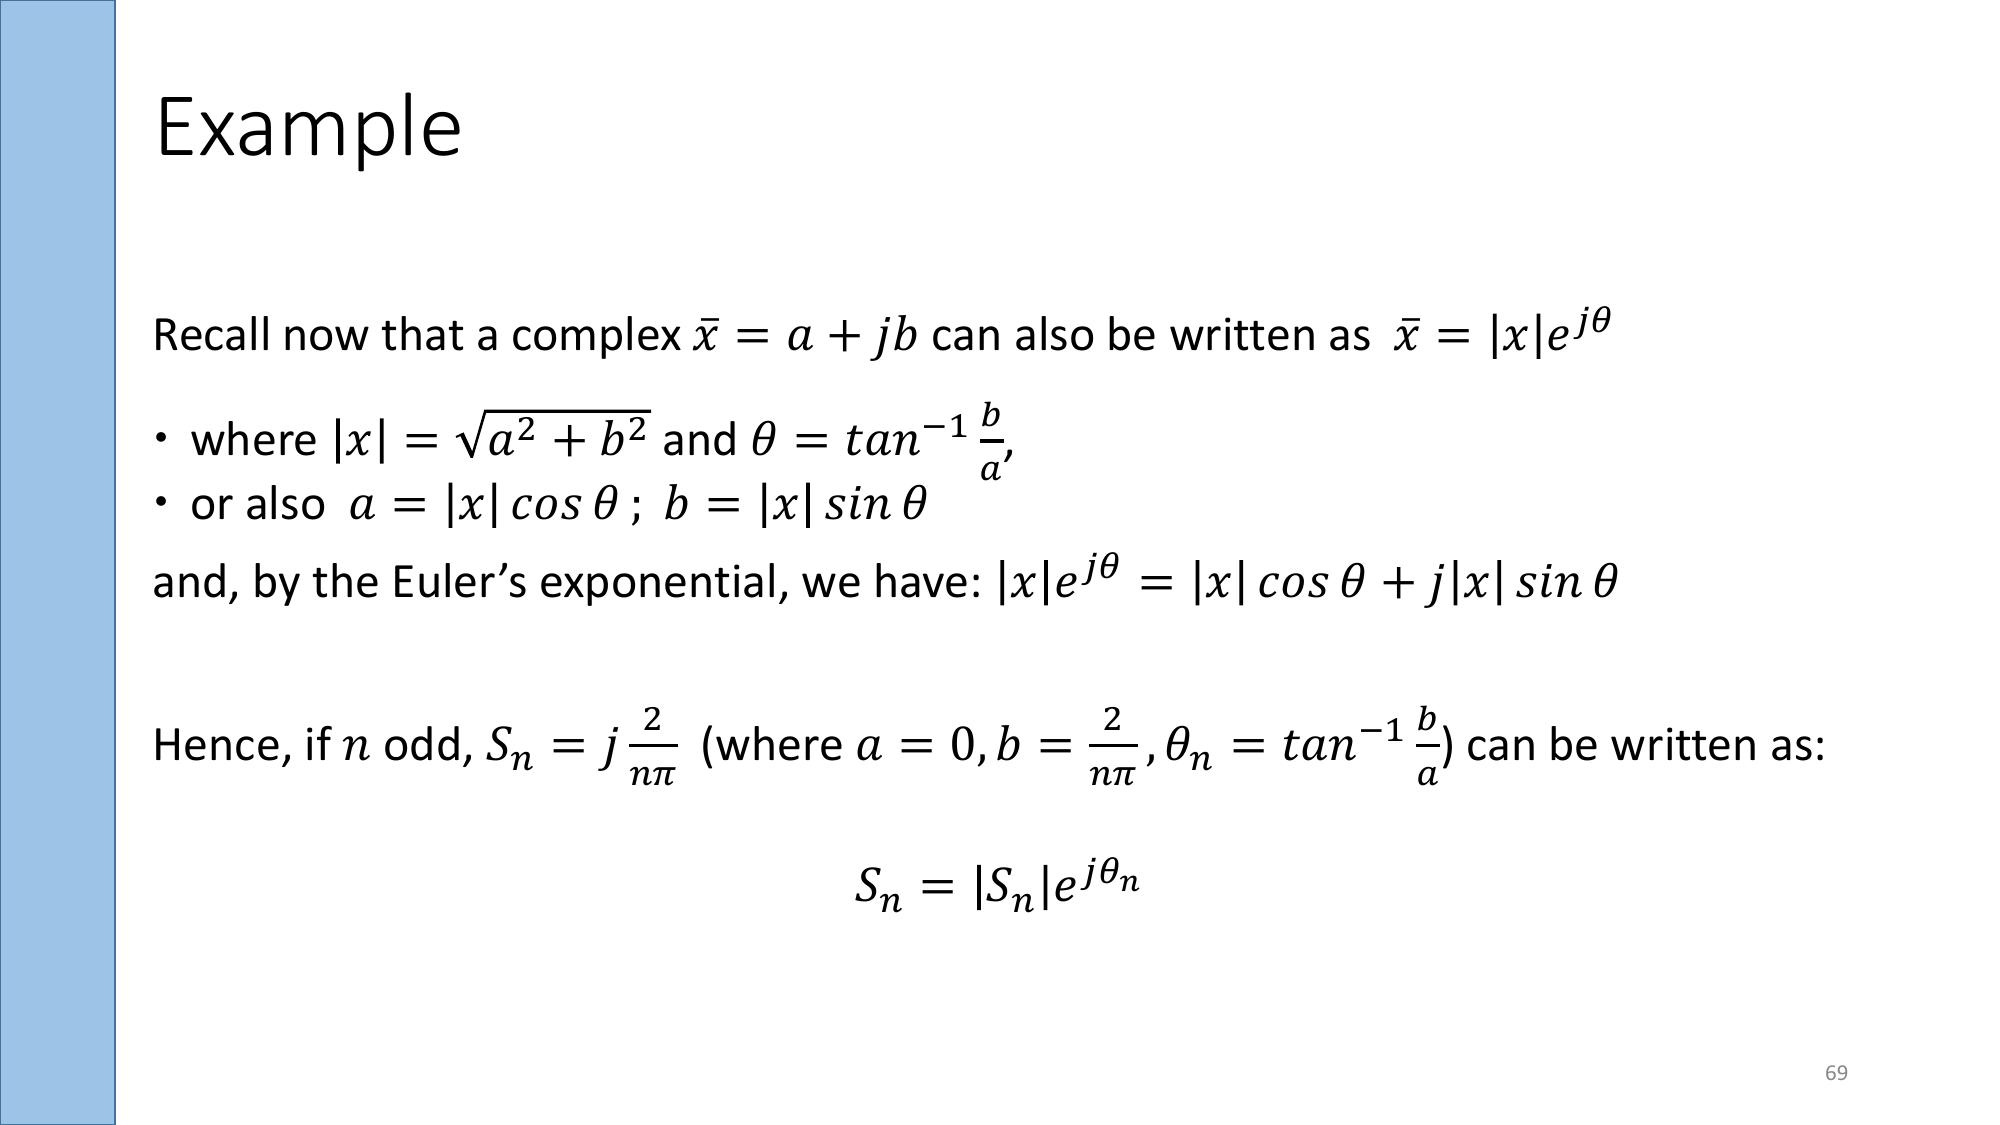
\includegraphics[keepaspectratio]{images/lezione-25-lab-teoria-dei-segnali-introduzione-e-serie-di-fourier-img-06.jpg}}
\caption{Al crescere del numero di armoniche considerate (verde → rosso
→ blu) la serie converge all'onda rettangolare. La forma in blu con
k=100 è quasi perfetta, con il solo fenomeno di Gibbs ai salti.}
\end{figure}

\begin{center}\rule{0.5\linewidth}{0.5pt}\end{center}

\section{Lo Spettro di un Segnale}\label{lo-spettro-di-un-segnale}

La sequenza ordinata dei coefficienti \(\{S_n\}_{n=-\infty}^{+\infty}\)
è chiamata \textbf{spettro} del segnale. Conoscere lo spettro equivale a
conoscere il segnale (dove \(s(t)\) è continua; nei punti di
discontinuità vale la media dei limiti laterali, per il teorema di
Dirichlet).

Poiché i coefficienti \(S_n\) sono in generale numeri complessi anche
quando \(s(t)\) è reale, lo spettro non può essere rappresentato con un
singolo grafico 2D. Si usano invece due diagrammi separati, sfruttando
la rappresentazione \(S_n = |S_n| e^{j\theta_n}\):

\begin{itemize}
\tightlist
\item
  \textbf{Spettro di ampiezza}: il grafico di \(|S_n|\) in funzione di
  \(n\) (o della frequenza \(nF\))
\item
  \textbf{Spettro di fase}: il grafico di \(\theta_n = \arg(S_n)\) in
  funzione di \(n\)
\end{itemize}

\begin{callouttip}{Spettro dell’onda quadra antisimmetrica}

Per il segnale \(s(t) = -1\) se \(0 < t \le T/2\), \(s(t) = 1\) se
\(T/2 < t \le T\), i coefficienti sono:
\[S_n = \begin{cases} 0 & n \text{ pari} \\ \dfrac{2}{n\pi} e^{j\pi/2} & n > 0, \text{ dispari} \\ -\dfrac{2}{n\pi} e^{-j\pi/2} & n < 0, \text{ dispari} \end{cases}\]
Lo spettro di ampiezza decade come \(2/(|n|\pi)\) per gli indici
dispari; lo spettro di fase è costante a \(+\pi/2\) per \(n > 0\) e
\(-\pi/2\) per \(n < 0\).

\end{callouttip}

\begin{center}\rule{0.5\linewidth}{0.5pt}\end{center}

\section{Segnali Aperiodici e Supporto
Limitato}\label{segnali-aperiodici-e-supporto-limitato}

Anche per i segnali aperiodici con supporto limitato a \([a, b)\) ---
cioè \(s(t) = 0\) per \(t \notin [a,b)\) --- è possibile calcolare la
serie di Fourier. Tuttavia, la serie assume implicitamente che il
segnale sia periodico con periodo \(T = b - a\). La conseguenza è che,
invertendo la serie (da \(S_n\) a \(s(t)\)), si ottiene
l'\textbf{estensione periodica} del segnale originale, non il segnale
aperiodico stesso.

\[s^*(t) = \sum_{n=-\infty}^{+\infty} s(t - nT)\]

Questo passaggio è cruciale: la serie di Fourier non può rappresentare
segnali davvero aperiodici. Per questi occorre la \textbf{Trasformata di
Fourier}, che è in un certo senso il limite della serie di Fourier per
\(T \to \infty\).

\begin{center}\rule{0.5\linewidth}{0.5pt}\end{center}

\section{Trasformata di Fourier}\label{trasformata-di-fourier}

\subsection{Dal Discreto al Continuo: Passaggio dalla Serie alla
Trasformata}\label{dal-discreto-al-continuo-passaggio-dalla-serie-alla-trasformata}

La serie di Fourier funziona bene per segnali periodici: rappresenta il
segnale come somma di armoniche a frequenze discrete \(nF = n/T\). Ma la
stragrande maggioranza dei segnali reali di interesse --- impulsi,
transitori, frammenti audio, burst radio --- non sono periodici. Come
estendere l'analisi in frequenza a questi segnali?

L'idea è elegante: si considera il segnale non periodico come il limite
di un segnale periodico il cui periodo \(T\) tende all'infinito. Quando
\(T\) cresce, la frequenza fondamentale \(F = 1/T\) diminuisce, e le
armoniche discrete \(nF\) si avvicinano sempre di più tra loro. Nel
limite \(T \to \infty\), la spaziatura tra le armoniche
\(\Delta_f = 1/T \to 0\) e lo spettro discreto diventa uno
\textbf{spettro continuo}.

\begin{figure}
\centering
\pandocbounded{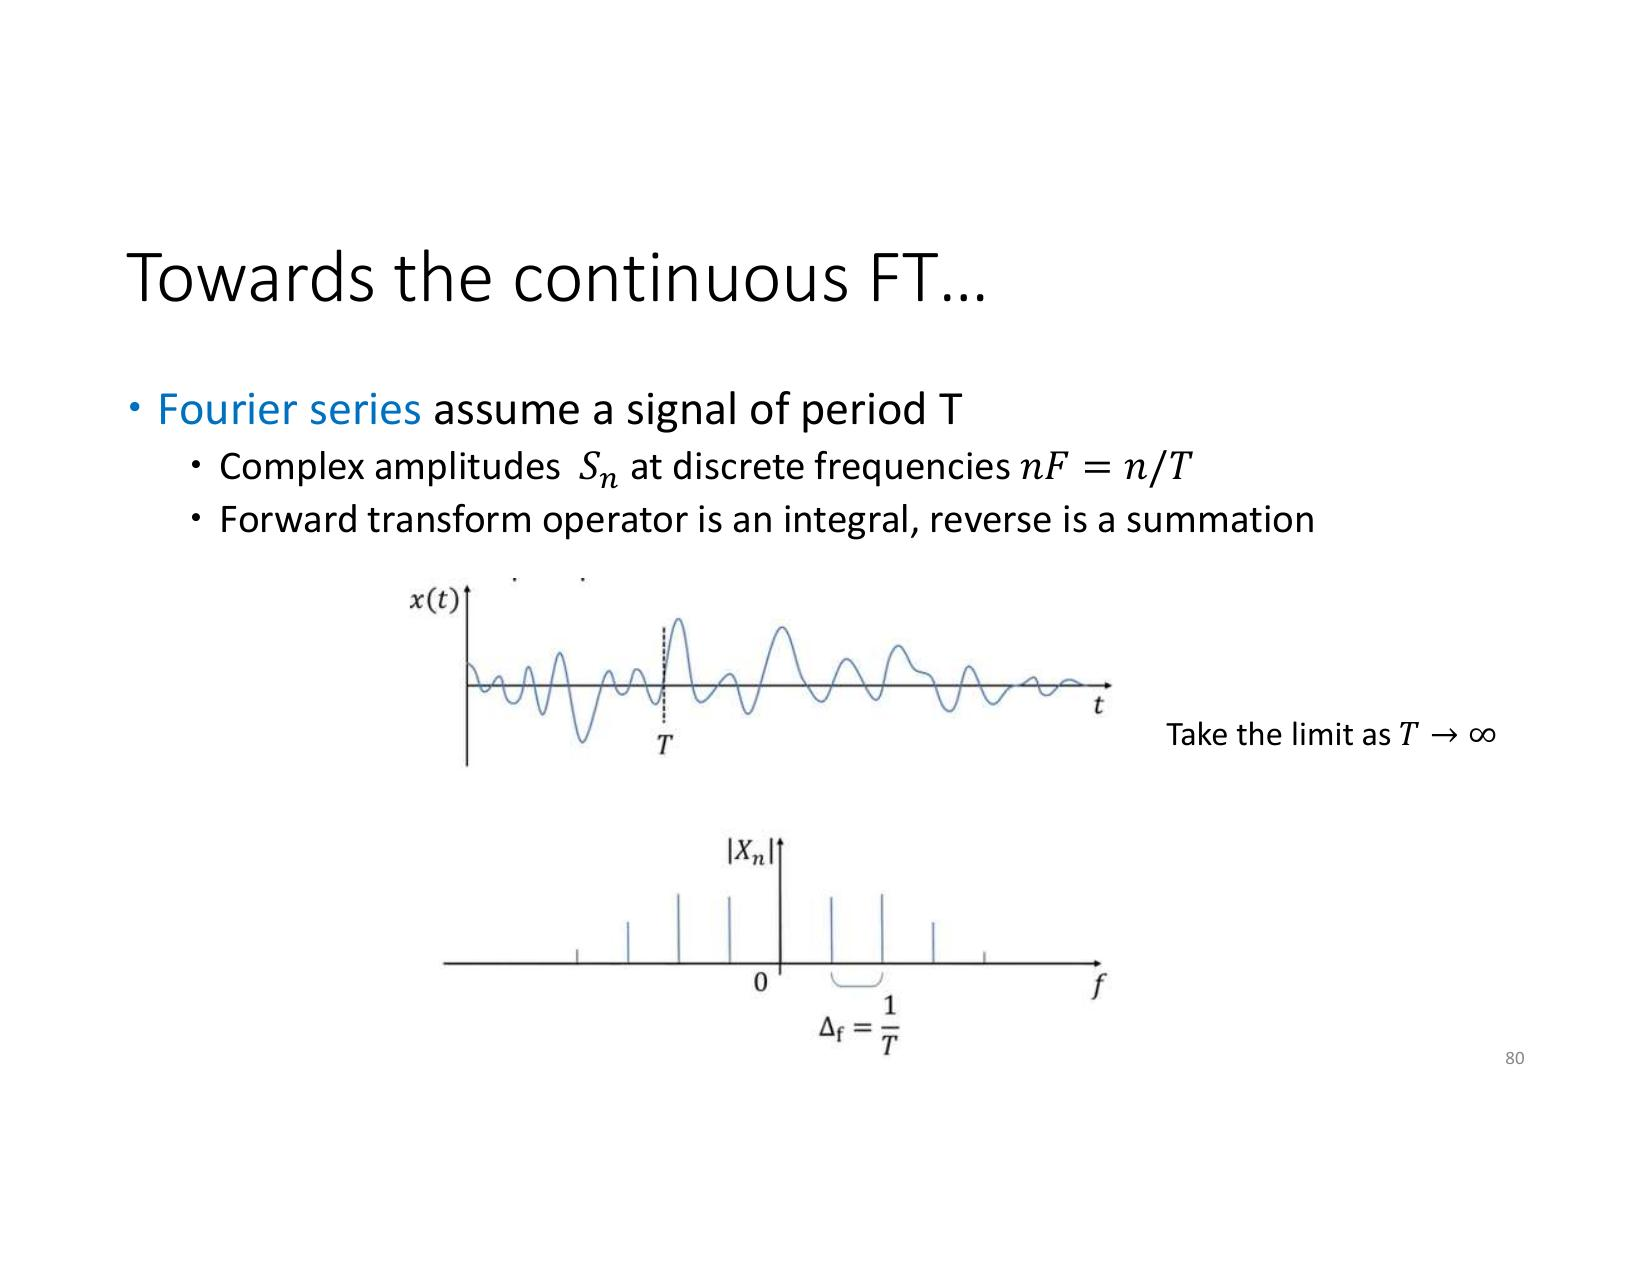
\includegraphics[keepaspectratio]{images/lezione-27-lab-teoria-dei-segnali-trasformata-di-fourier-campionamento-e-dft-img-01.jpg}}
\caption{Segnale periodico e relativo spettro discreto. All'aumentare di
T, le righe spettrali si avvicinano. Prendendo il limite T→∞ si ottiene
lo spettro continuo.}
\end{figure}

\begin{figure}
\centering
\pandocbounded{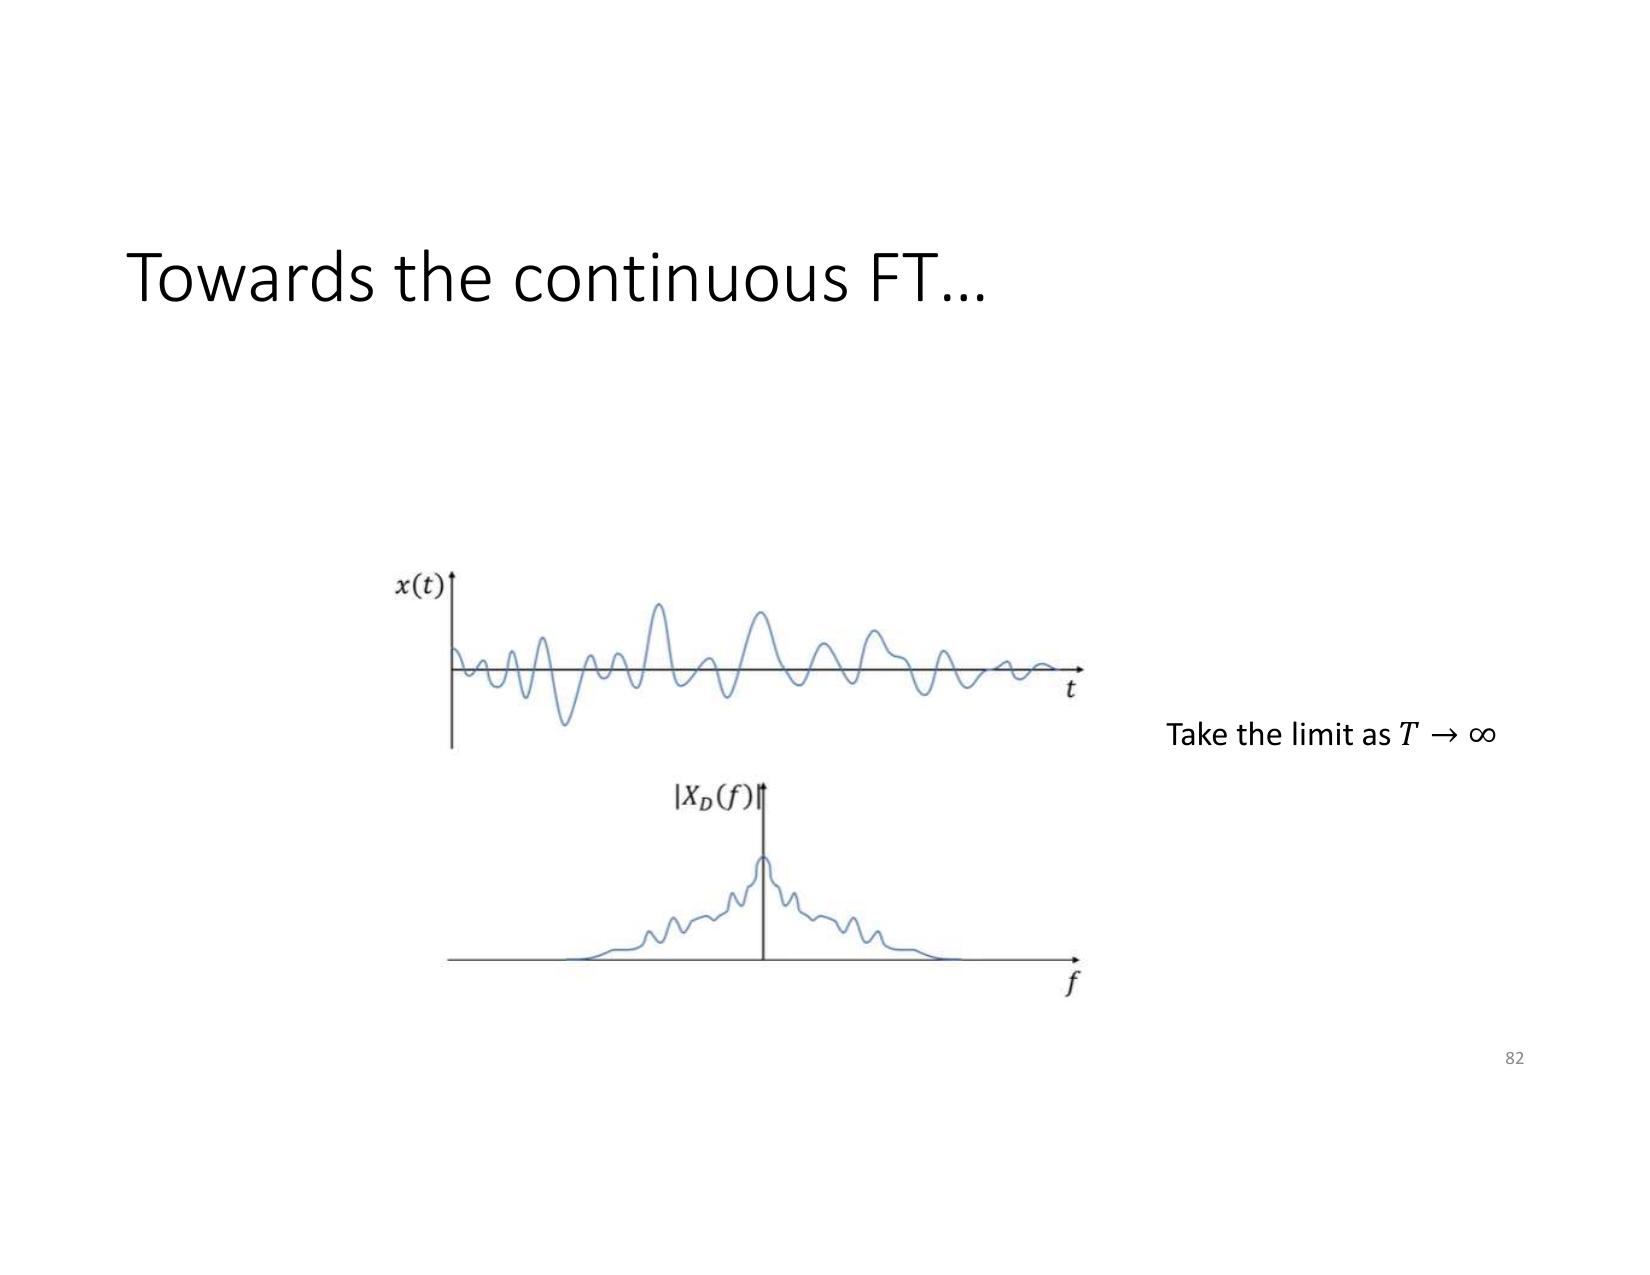
\includegraphics[keepaspectratio]{images/lezione-27-lab-teoria-dei-segnali-trasformata-di-fourier-campionamento-e-dft-img-02.jpg}}
\caption{Quando T→∞, il segnale ``dimentica'' la propria periodicità e
lo spettro \textbar X\_D(f)\textbar{} diventa una funzione continua
della frequenza.}
\end{figure}

\begin{calloutdefinition}{Trasformata Continua di Fourier (CFT)}

Un segnale non periodico \(s(t)\) può essere espresso come:

\[s(t) = \int_{-\infty}^{+\infty} S(f)\, e^{j2\pi ft}\, df\]

dove \(S(f)\) è la \textbf{densità spettrale complessa}, data dalla
trasformata diretta:

\[S(f) = \mathcal{F}(s(t)) = \int_{-\infty}^{+\infty} s(t)\, e^{-j2\pi ft}\, dt\]

Si scrive in forma compatta \(s(t) \Longleftrightarrow S(f)\).

\end{calloutdefinition}

A differenza della serie di Fourier --- che produce un insieme
\textbf{discreto} di coefficienti \(S_n\) --- la CFT produce uno spettro
\textbf{continuo} \(S(f)\) definito su tutte le frequenze reali
\(f \in (-\infty, +\infty)\).

\subsection{Esempio: Segnale Pulsato}\label{esempio-segnale-pulsato}

Consideriamo il segnale rettangolare:

\[s(t) = \begin{cases} 1 & \text{se } |t| \leq T/2 \\ 0 & \text{altrimenti} \end{cases}\]

La sua trasformata continua di Fourier si calcola analiticamente:

\[S(f) = \int_{-T/2}^{T/2} e^{-j2\pi ft}\, dt = T \cdot \text{sinc}(\pi f T) = \frac{\sin(\pi f T)}{\pi f}\]

Il risultato è una funzione \textbf{sinc} nel dominio della frequenza.
Un fatto cruciale è che all'aumentare di \(T\) (impulso più largo nel
tempo), lo spettro si restringe in frequenza, e viceversa. Questo è il
principio di \textbf{incertezza tempo-frequenza}: un segnale non può
essere contemporaneamente concentrato sia nel tempo che in frequenza.

\begin{figure}
\centering
\pandocbounded{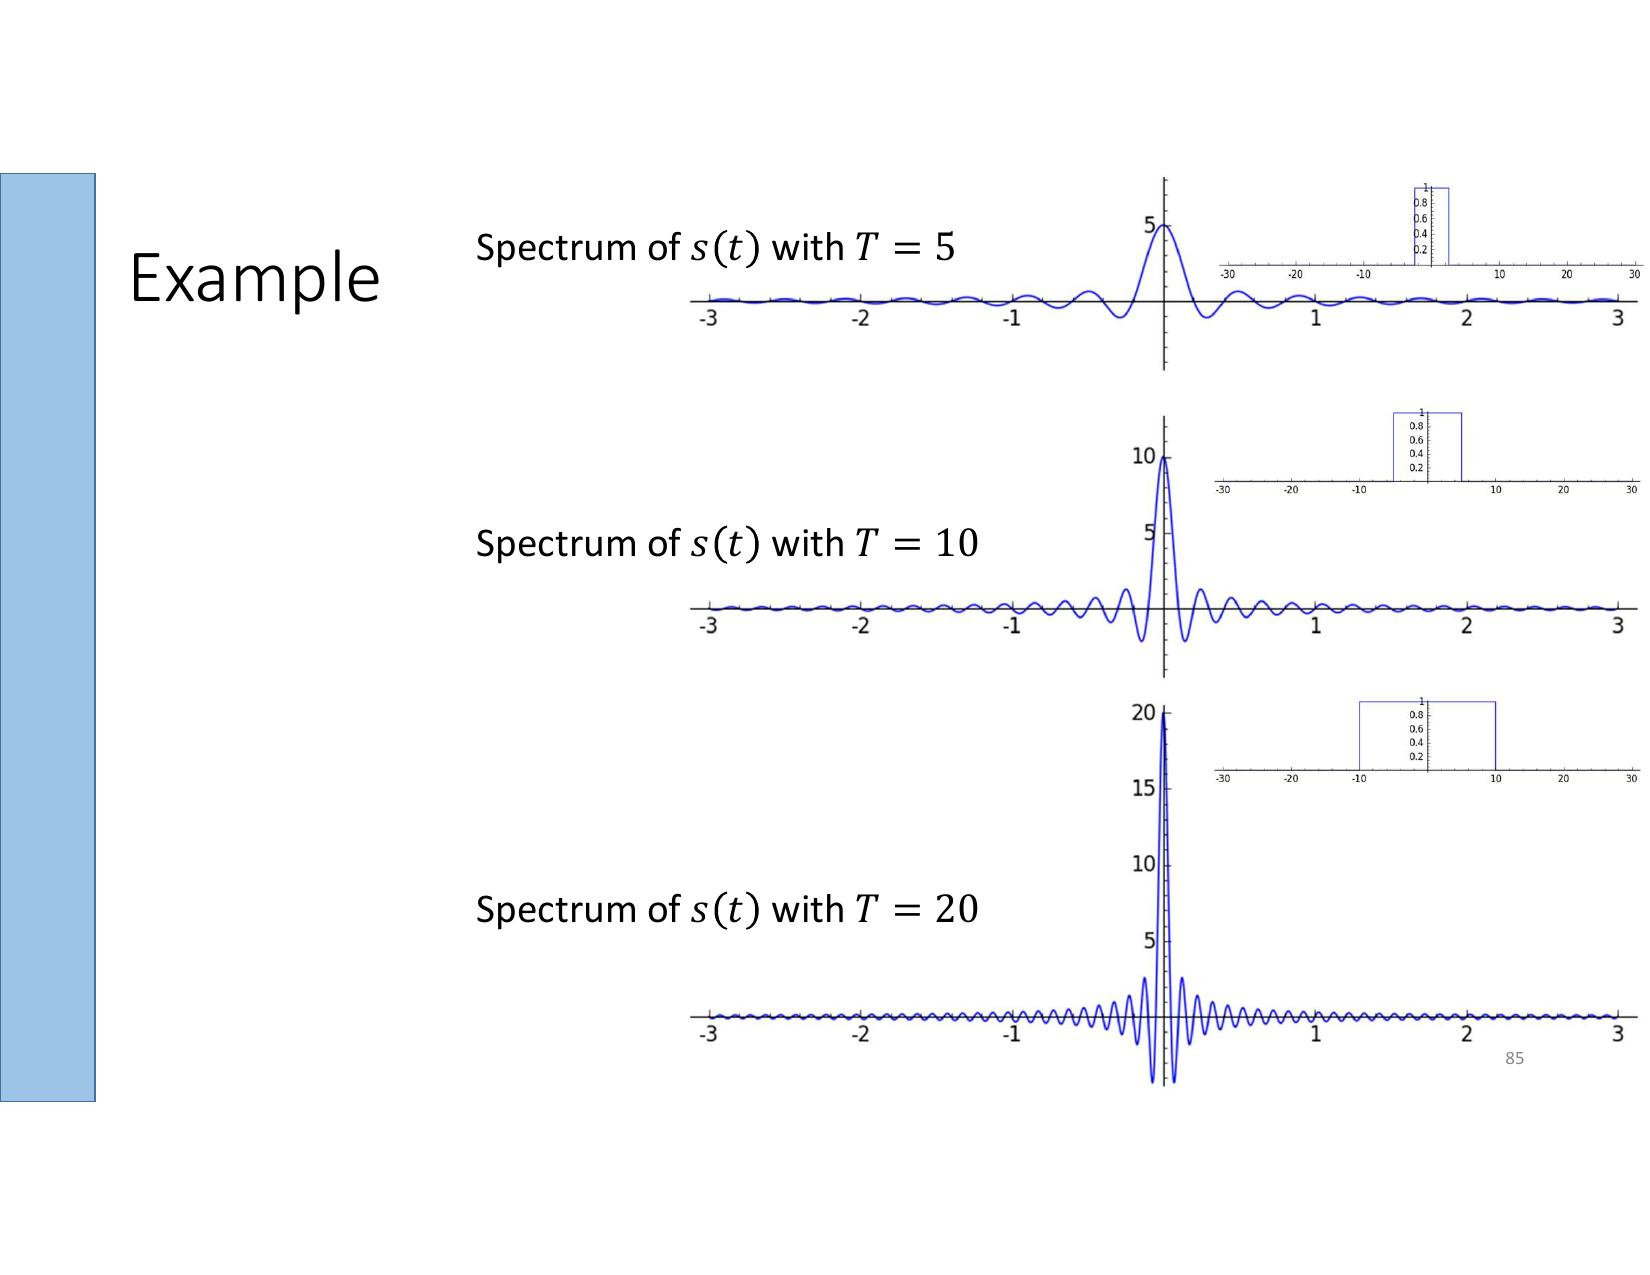
\includegraphics[keepaspectratio]{images/lezione-27-lab-teoria-dei-segnali-trasformata-di-fourier-campionamento-e-dft-img-03.jpg}}
\caption{Spettri del segnale pulsato al variare della durata T.
All'aumentare di T il lobo principale della sinc si restringe,
riflettendo il principio di incertezza tempo-frequenza.}
\end{figure}

\begin{figure}
\centering
\pandocbounded{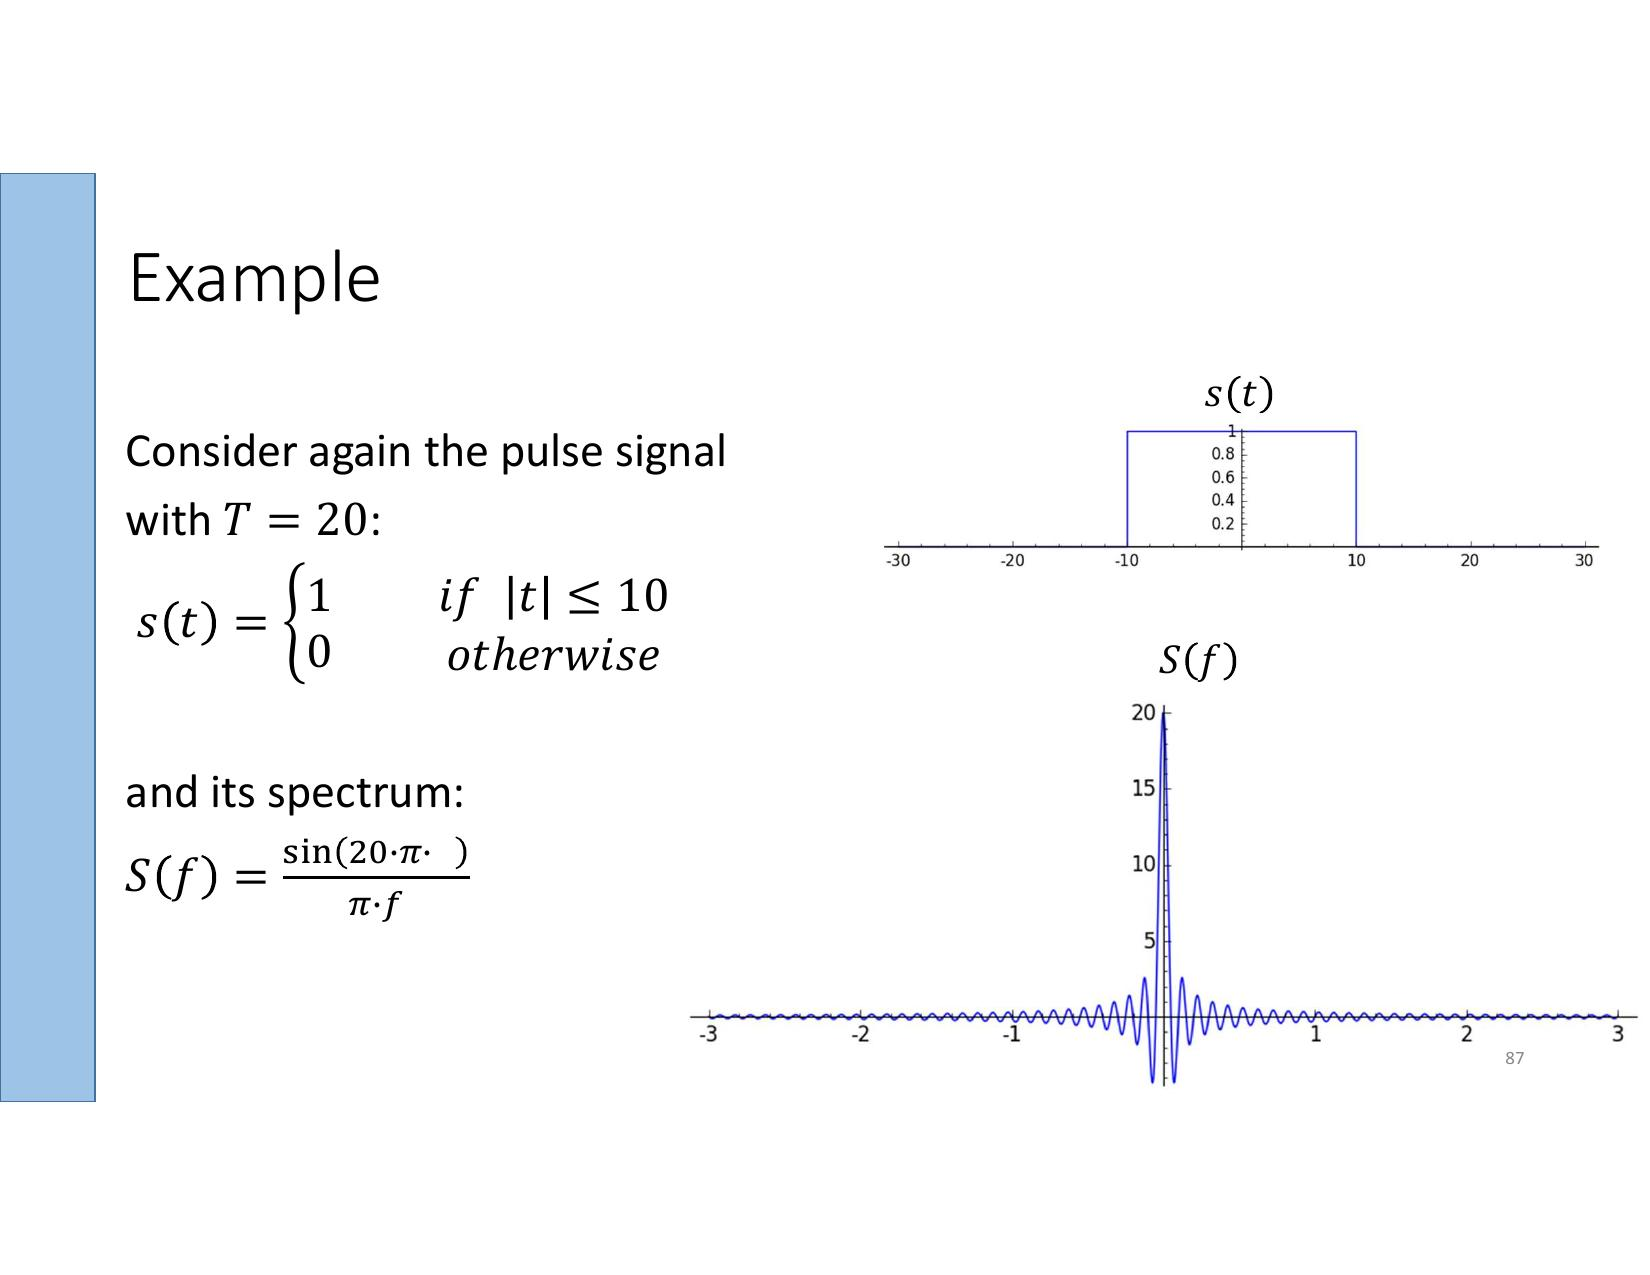
\includegraphics[keepaspectratio]{images/lezione-27-lab-teoria-dei-segnali-trasformata-di-fourier-campionamento-e-dft-img-04.jpg}}
\caption{Segnale pulsato con T=20: il segnale nel dominio del tempo
(rettangolo di ampiezza 1 e durata 20) e il corrispondente spettro
S(f)=sin(20πf)/(πf).}
\end{figure}

\subsection{Banda di un Segnale e
Filtraggio}\label{banda-di-un-segnale-e-filtraggio}

Lo spettro di un segnale generico si estende su tutte le frequenze in
\((-\infty, +\infty)\). Tuttavia, nella pratica non tutte le componenti
frequenziali sono ugualmente utili o necessarie. Filtrare un segnale
significa \textbf{selezionare un sottoinsieme delle sue componenti
spettrali}. Le motivazioni principali sono:

\begin{itemize}
\tightlist
\item
  alcune frequenze contengono l'informazione rilevante, altre
  corrispondono a rumore o interferenze
\item
  i canali di comunicazione hanno banda disponibile limitata
\item
  si vuole separare segnali che si sovrappongono in frequenza
\end{itemize}

I filtri principali sono: - \textbf{Filtro passa-basso}
(\emph{low-pass}): lascia passare le frequenze sotto una soglia \(f_c\),
blocca le alte frequenze - \textbf{Filtro passa-alto}
(\emph{high-pass}): lascia passare le frequenze sopra \(f_c\), blocca le
basse - \textbf{Filtro passa-banda} (\emph{band-pass}): lascia passare
le frequenze in un intervallo \([f_1, f_2]\)

\begin{callouttip}{Filtraggio del segnale pulsato}

Consideriamo il segnale rettangolare con \(T=20\) e il suo spettro
\(S(f) = \sin(20\pi f)/(\pi f)\).

\end{callouttip}

\begin{figure}
\centering
\pandocbounded{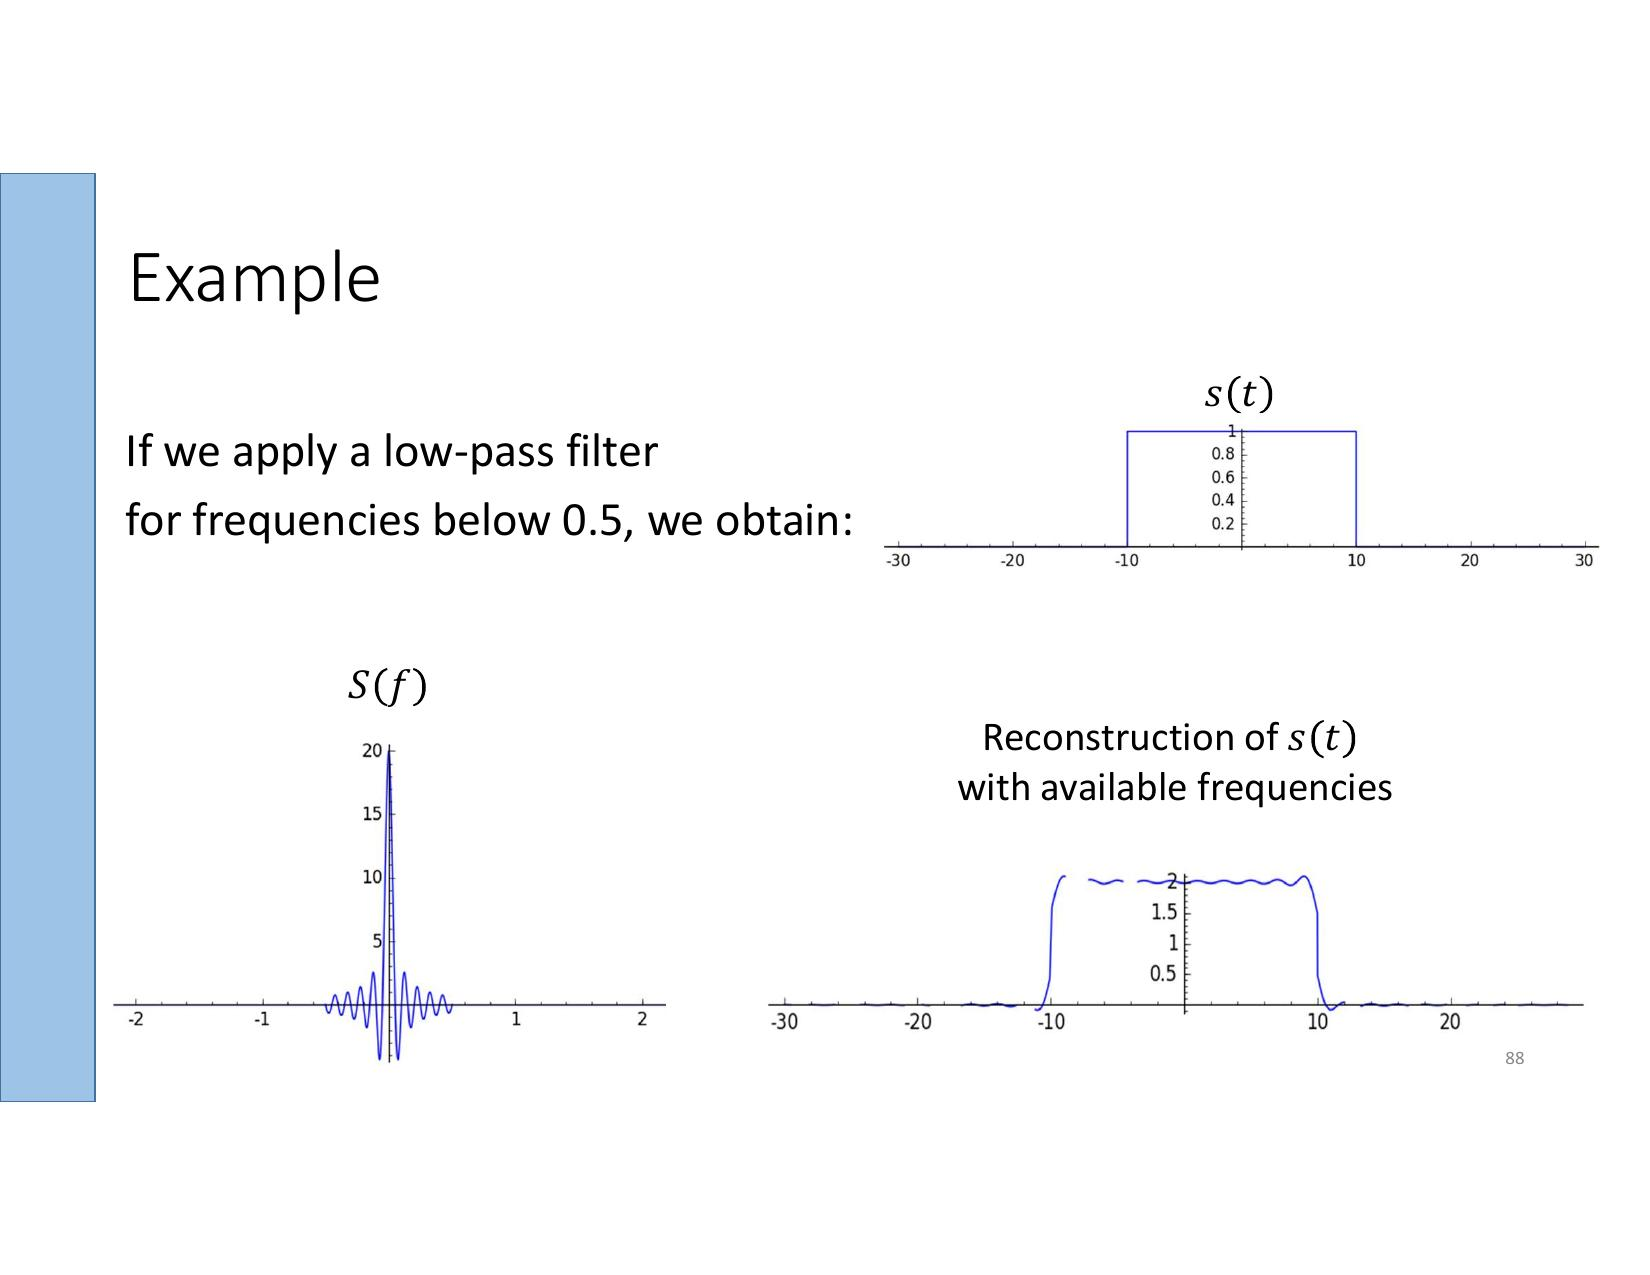
\includegraphics[keepaspectratio]{images/lezione-27-lab-teoria-dei-segnali-trasformata-di-fourier-campionamento-e-dft-img-05.jpg}}
\caption{Filtro passa-basso (soglia 0.5 Hz): lo spettro viene troncato
alle basse frequenze. La ricostruzione nel dominio del tempo riproduce
approssimativamente la forma del rettangolo, con arrotondamento agli
spigoli.}
\end{figure}

\begin{figure}
\centering
\pandocbounded{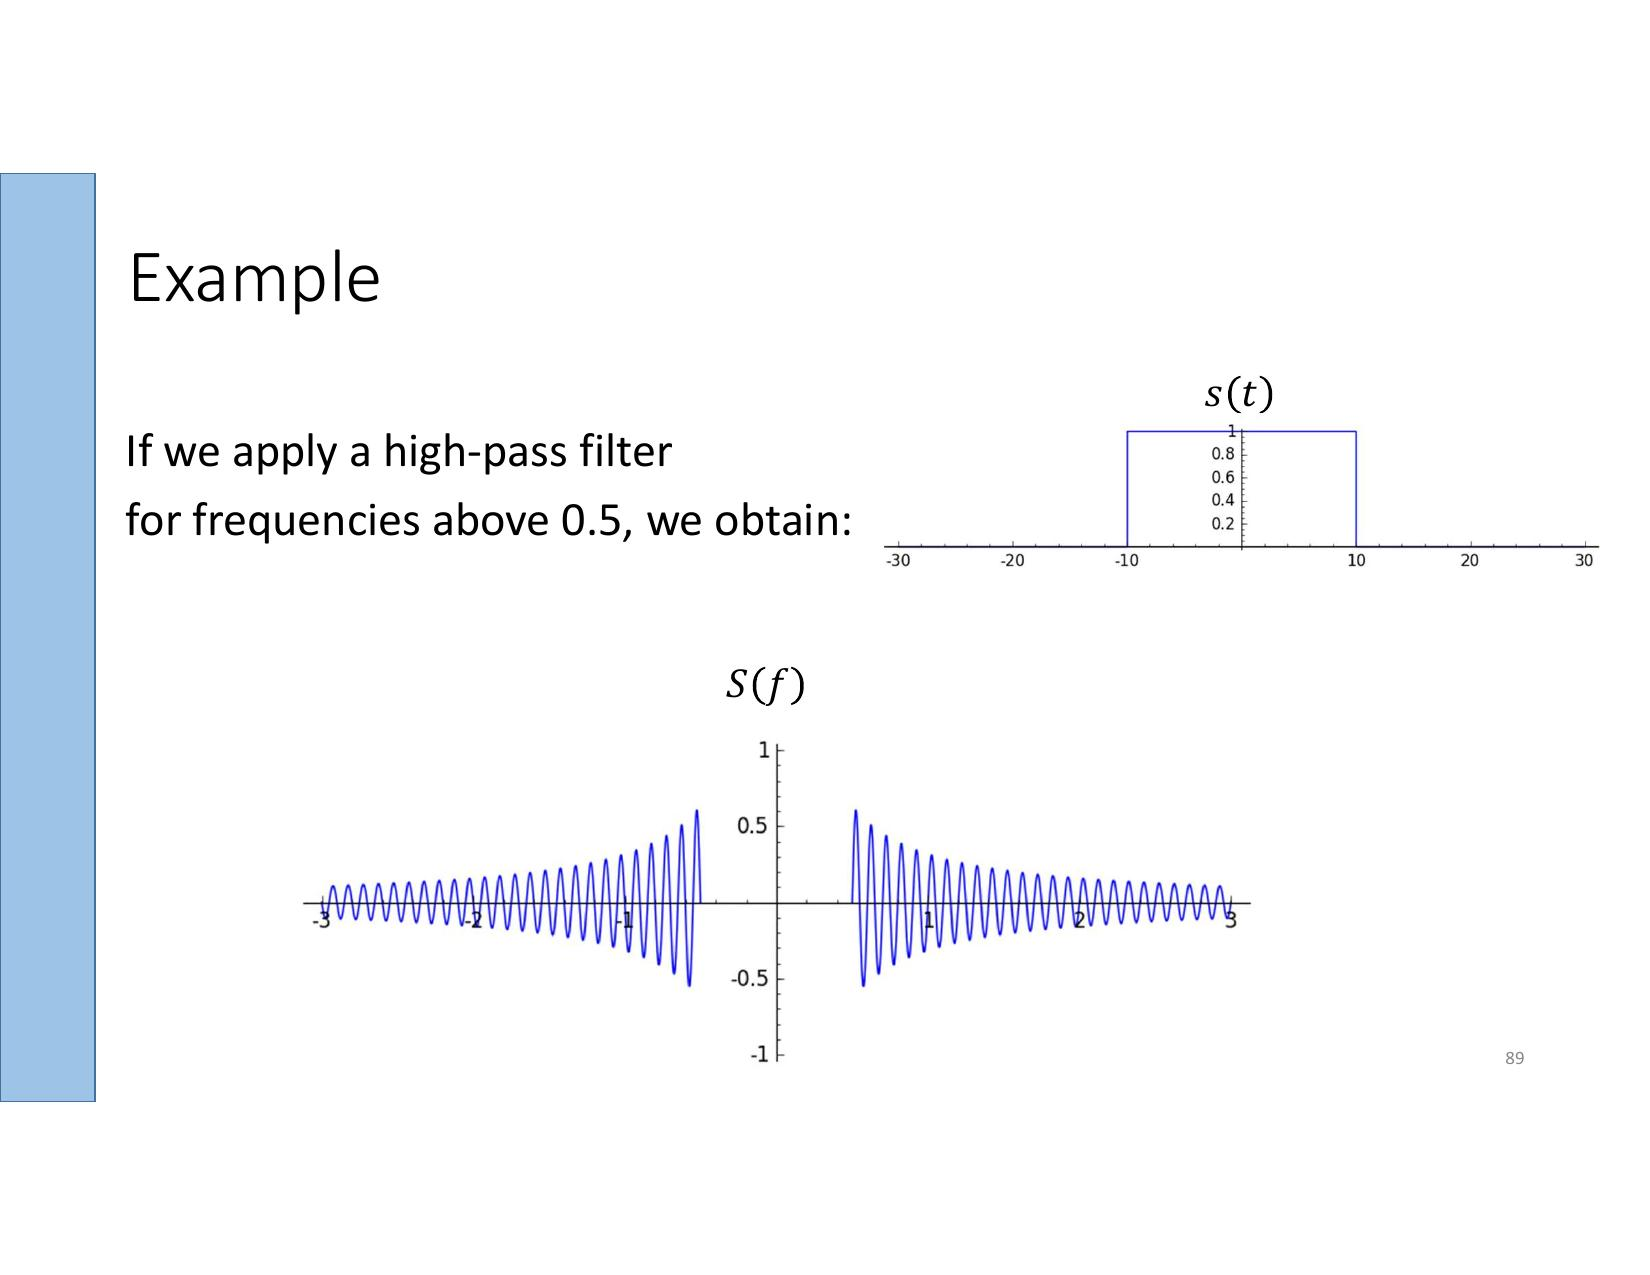
\includegraphics[keepaspectratio]{images/lezione-27-lab-teoria-dei-segnali-trasformata-di-fourier-campionamento-e-dft-img-06.jpg}}
\caption{Filtro passa-alto (soglia 0.5 Hz): rimangono solo le componenti
ad alta frequenza dello spettro. Il segnale ricostruito ha una forma
oscillatoria concentrata ai bordi del rettangolo originale.}
\end{figure}

\begin{figure}
\centering
\pandocbounded{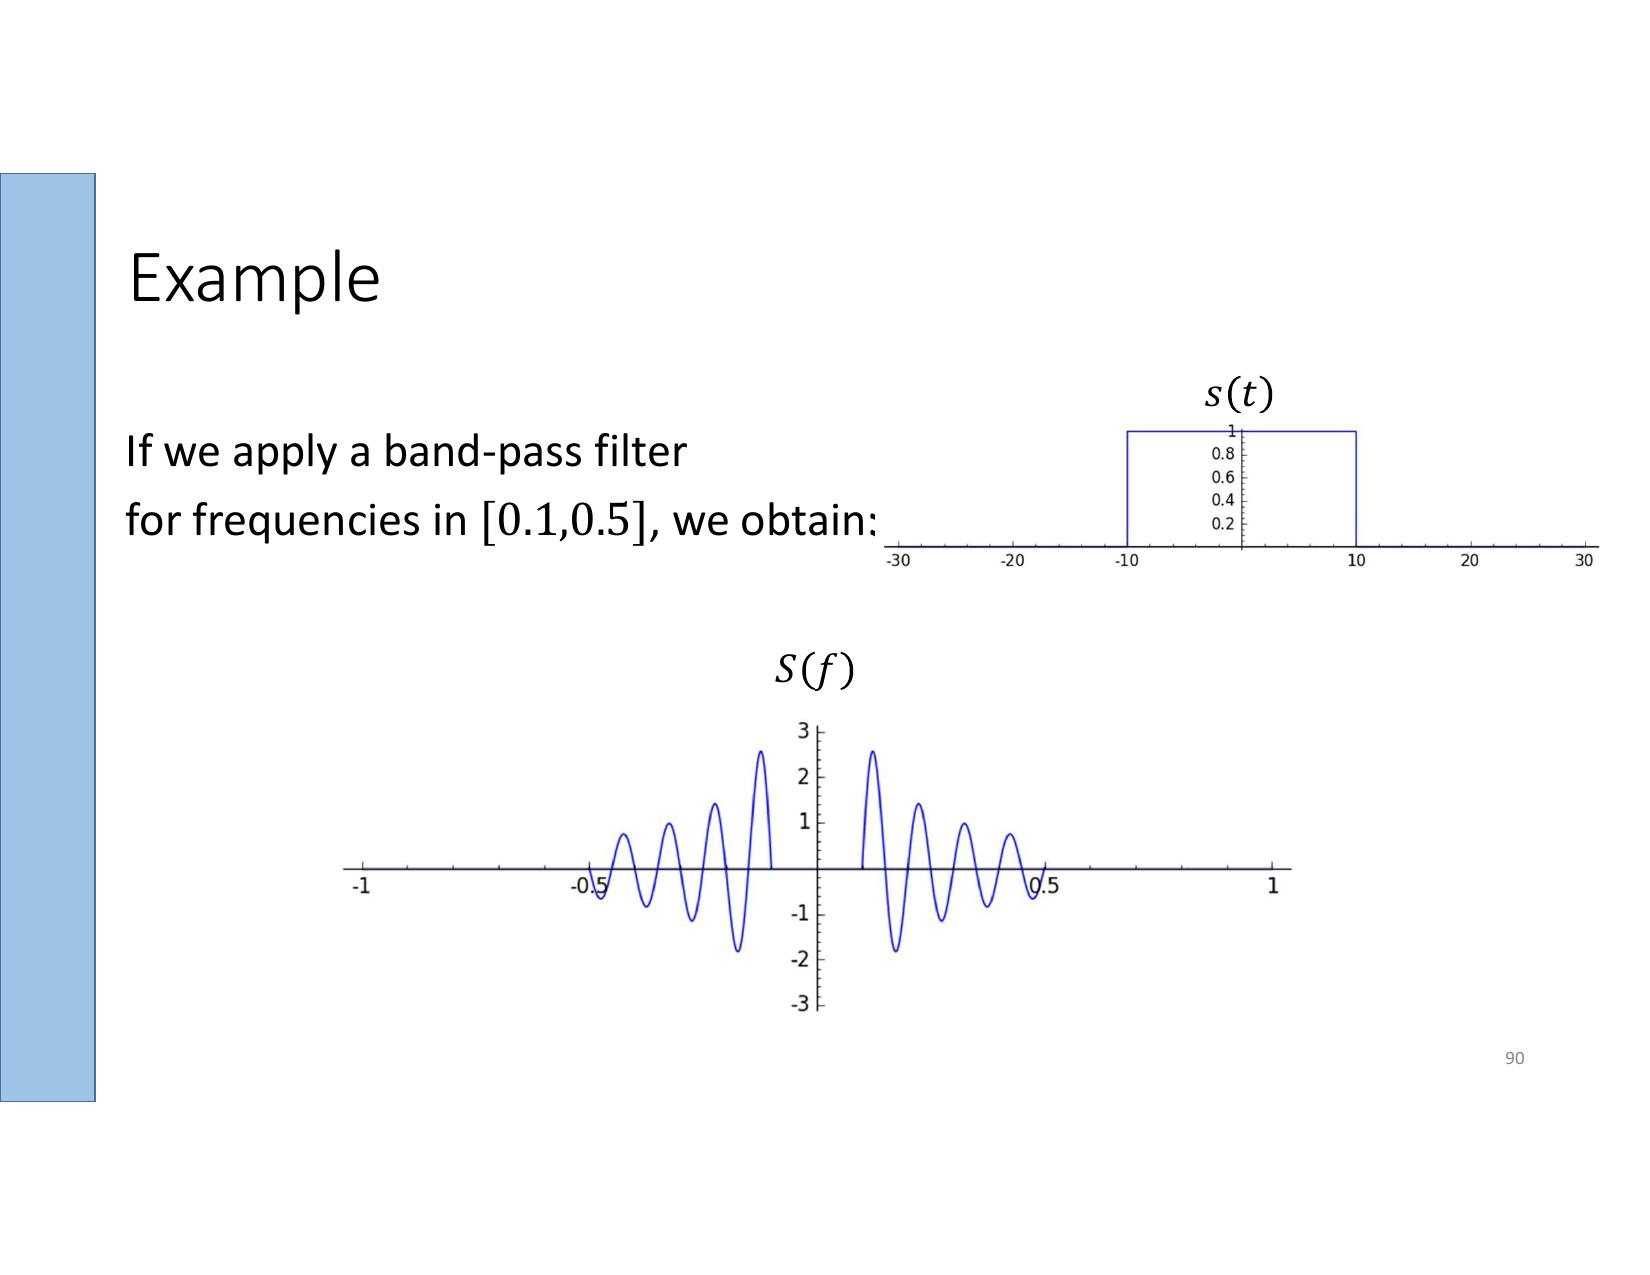
\includegraphics[keepaspectratio]{images/lezione-27-lab-teoria-dei-segnali-trasformata-di-fourier-campionamento-e-dft-img-07.jpg}}
\caption{Filtro passa-banda (intervallo {[}0.1, 0.5{]} Hz): vengono
selezionate le componenti in una fascia di frequenze. Il risultato è un
segnale oscillante.}
\end{figure}

\begin{callouttip}{Intuizione sul filtraggio}

Applicare un filtro nel dominio della frequenza equivale a moltiplicare
lo spettro \(S(f)\) per la risposta del filtro \(H(f)\). Nel dominio del
tempo questo corrisponde a una convoluzione del segnale con la risposta
impulsiva del filtro. Le basse frequenze determinano il ``contorno
grossolano'' del segnale; le alte frequenze determinano i dettagli fini
e gli spigoli.

\end{callouttip}

\subsection{Confronto: Serie di Fourier vs
Trasformata}\label{confronto-serie-di-fourier-vs-trasformata}

{\def\LTcaptype{none} % do not increment counter
\begin{longtable}[]{@{}
  >{\raggedright\arraybackslash}p{(\linewidth - 4\tabcolsep) * \real{0.3333}}
  >{\raggedright\arraybackslash}p{(\linewidth - 4\tabcolsep) * \real{0.3333}}
  >{\raggedright\arraybackslash}p{(\linewidth - 4\tabcolsep) * \real{0.3333}}@{}}
\toprule\noalign{}
\begin{minipage}[b]{\linewidth}\raggedright
\end{minipage} & \begin{minipage}[b]{\linewidth}\raggedright
Serie di Fourier
\end{minipage} & \begin{minipage}[b]{\linewidth}\raggedright
Trasformata di Fourier
\end{minipage} \\
\midrule\noalign{}
\endhead
\bottomrule\noalign{}
\endlastfoot
Tipo di segnale & Periodico & Non periodico \\
Spettro & Discreto (coefficienti \(S_n\)) & Continuo (\(S(f)\)) \\
Output & Insieme di coefficienti & Funzione continua di frequenza \\
Esempi tipici & Onda quadra, sinusoidi & Impulsi, transienti, frammenti
audio \\
\end{longtable}
}

\begin{center}\rule{0.5\linewidth}{0.5pt}\end{center}

\section{Da Segnale Analogico a Digitale: Campionamento e
Quantizzazione}\label{da-segnale-analogico-a-digitale-campionamento-e-quantizzazione}

I sistemi digitali moderni (computer, smartphone, dispositivi IoT)
lavorano esclusivamente con dati discreti. Un segnale analogico
continuo, come una voce o un sensore di temperatura, deve essere
convertito in una sequenza di valori discreti. Questo processo si
articola in due fasi: \textbf{campionamento} e \textbf{quantizzazione}.

\begin{figure}
\centering
\pandocbounded{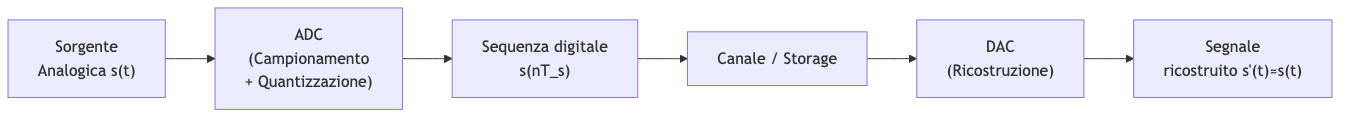
\includegraphics[keepaspectratio,alt={Pipeline di conversione analogico-digitale e digitale-analogica. L'ADC introduce inevitabilmente un errore di quantizzazione; il DAC ricostruisce un'approssimazione del segnale originale.}]{images/mermaid-02-teoria-dei-segnali-01.png}}
\caption{Pipeline di conversione analogico-digitale e
digitale-analogica. L'ADC introduce inevitabilmente un errore di
quantizzazione; il DAC ricostruisce un'approssimazione del segnale
originale.}
\end{figure}

\subsection{Campionamento}\label{campionamento}

\textbf{Campionare} un segnale \(s(t)\) significa estrarre i valori che
il segnale assume a istanti discreti regolarmente spaziati. Il parametro
chiave è il \textbf{periodo di campionamento} \(T_s\) (o
equivalentemente la \textbf{frequenza di campionamento}
\(f_s = 1/T_s\)):

\[g(nT_s) = s(nT_s), \quad n \in \mathbb{Z}\]

Il risultato è una sequenza di numeri reali. A differenza della
quantizzazione, il campionamento --- sotto opportune ipotesi --- non
introduce perdita di informazione.

\subsection{Quantizzazione}\label{quantizzazione}

Mentre il campionamento opera sull'asse del tempo, la quantizzazione
opera sull'asse dell'ampiezza: trasforma ogni campione reale
\(x \in \mathbb{R}\) in un valore intero \(y \in [0, 2^R - 1]\), dove
\(R\) è il numero di bit del quantizzatore. Si usa un
\textbf{quantizzatore scalare a \(R\) bit}:

\begin{itemize}
\tightlist
\item
  la \textbf{risoluzione} per un segnale con valori in \([0, M]\) è
  \(M / 2^R\)
\item
  il \textbf{bitrate} di una sorgente campionata a \(f_s\) e quantizzata
  a \(R\) bit è: \(B = R \cdot f_s\) bit/s
\end{itemize}

\begin{calloutwarning}{Errore di quantizzazione}

La quantizzazione introduce un errore irreversibile: due valori
analogici diversi possono essere mappati allo stesso livello digitale.
Aumentare \(R\) riduce l'errore (migliore fedeltà), ma aumenta il
bitrate da trasmettere o memorizzare.

\end{calloutwarning}

\begin{callouttip}{Sistema telefonico analogico}

La voce umana ha un contenuto informativo utile fino a circa 4 kHz
(limite telefonico accettabile). Quindi: - frequenza di campionamento:
\(f_s = 8\) kHz (doppio di 4 kHz, come vedremo con Nyquist) -
quantizzazione su \(R = 8\) bit per campione - bitrate risultante:
\(B = 8 \times 8000 = 64\) kbps

\end{callouttip}

\subsection{Interpolazione e
Ricostruzione}\label{interpolazione-e-ricostruzione}

Dato un insieme di campioni, esistono vari metodi di ricostruzione del
segnale analogico: - \textbf{Zero-order hold}: ogni campione viene
``tenuto'' fino al successivo (segnale a gradini) - \textbf{First-order
hold}: interpolazione lineare tra campioni adiacenti -
\textbf{Interpolazione con seno cardinale} (\emph{sinc interpolation}):
metodo ottimale, usato nella dimostrazione del teorema di Nyquist

\begin{center}\rule{0.5\linewidth}{0.5pt}\end{center}

\section{Il Teorema di Campionamento di
Nyquist-Shannon}\label{il-teorema-di-campionamento-di-nyquist-shannon}

La domanda centrale della conversione A/D è: \textbf{a quale frequenza
minima devo campionare per poter ricostruire perfettamente il segnale
originale?}

\begin{callouttheorem}{Teorema di Nyquist-Shannon}

Sia \(s(t)\) un segnale con spettro nullo per frequenze superiori a
\(f_M\) (segnale \textbf{a banda limitata}). Allora \(s(t)\) è
completamente determinato dai suoi campioni presi all'intervallo:

\[T_s \leq \frac{1}{2f_M}\]

ovvero con frequenza di campionamento \(f_s \geq 2f_M\). La frequenza
minima \(f_N = 2f_M\) è chiamata \textbf{frequenza di Nyquist} o
\textbf{tasso di Nyquist}.

La ricostruzione esatta si ottiene tramite interpolazione con seno
cardinale:
\[s(t) = \sum_{n=-\infty}^{+\infty} s(nT_s) \cdot \frac{\sin(\pi f_s (t - nT_s))}{\pi f_s (t - nT_s)}\]

\end{callouttheorem}

Il teorema richiede che il segnale sia \textbf{strettamente a banda
limitata} --- condizione che, come vedremo, non è mai soddisfatta dai
segnali reali.

\begin{center}\rule{0.5\linewidth}{0.5pt}\end{center}

\section{Aliasing: Il Problema del
Sottocampionamento}\label{aliasing-il-problema-del-sottocampionamento}

Per capire cosa succede quando si campiona troppo lentamente, bisogna
guardare allo spettro del segnale campionato nel dominio della
frequenza.

\subsection{FT del Segnale Campionato}\label{ft-del-segnale-campionato}

Quando si campiona un segnale \(s(t)\) con frequenza \(f_s\), la
trasformata di Fourier del segnale campionato \textbf{consiste in
infinite repliche} dello spettro originale \(S(f)\), centrate alle
frequenze multiple di \(f_s\):

\[S_c(f) = f_s \sum_{k=-\infty}^{+\infty} S(f - kf_s)\]

La spaziatura tra le repliche è pari a \(f_s\): \textbf{più veloce è il
campionamento, più distanti sono le repliche}.

\begin{figure}
\centering
\pandocbounded{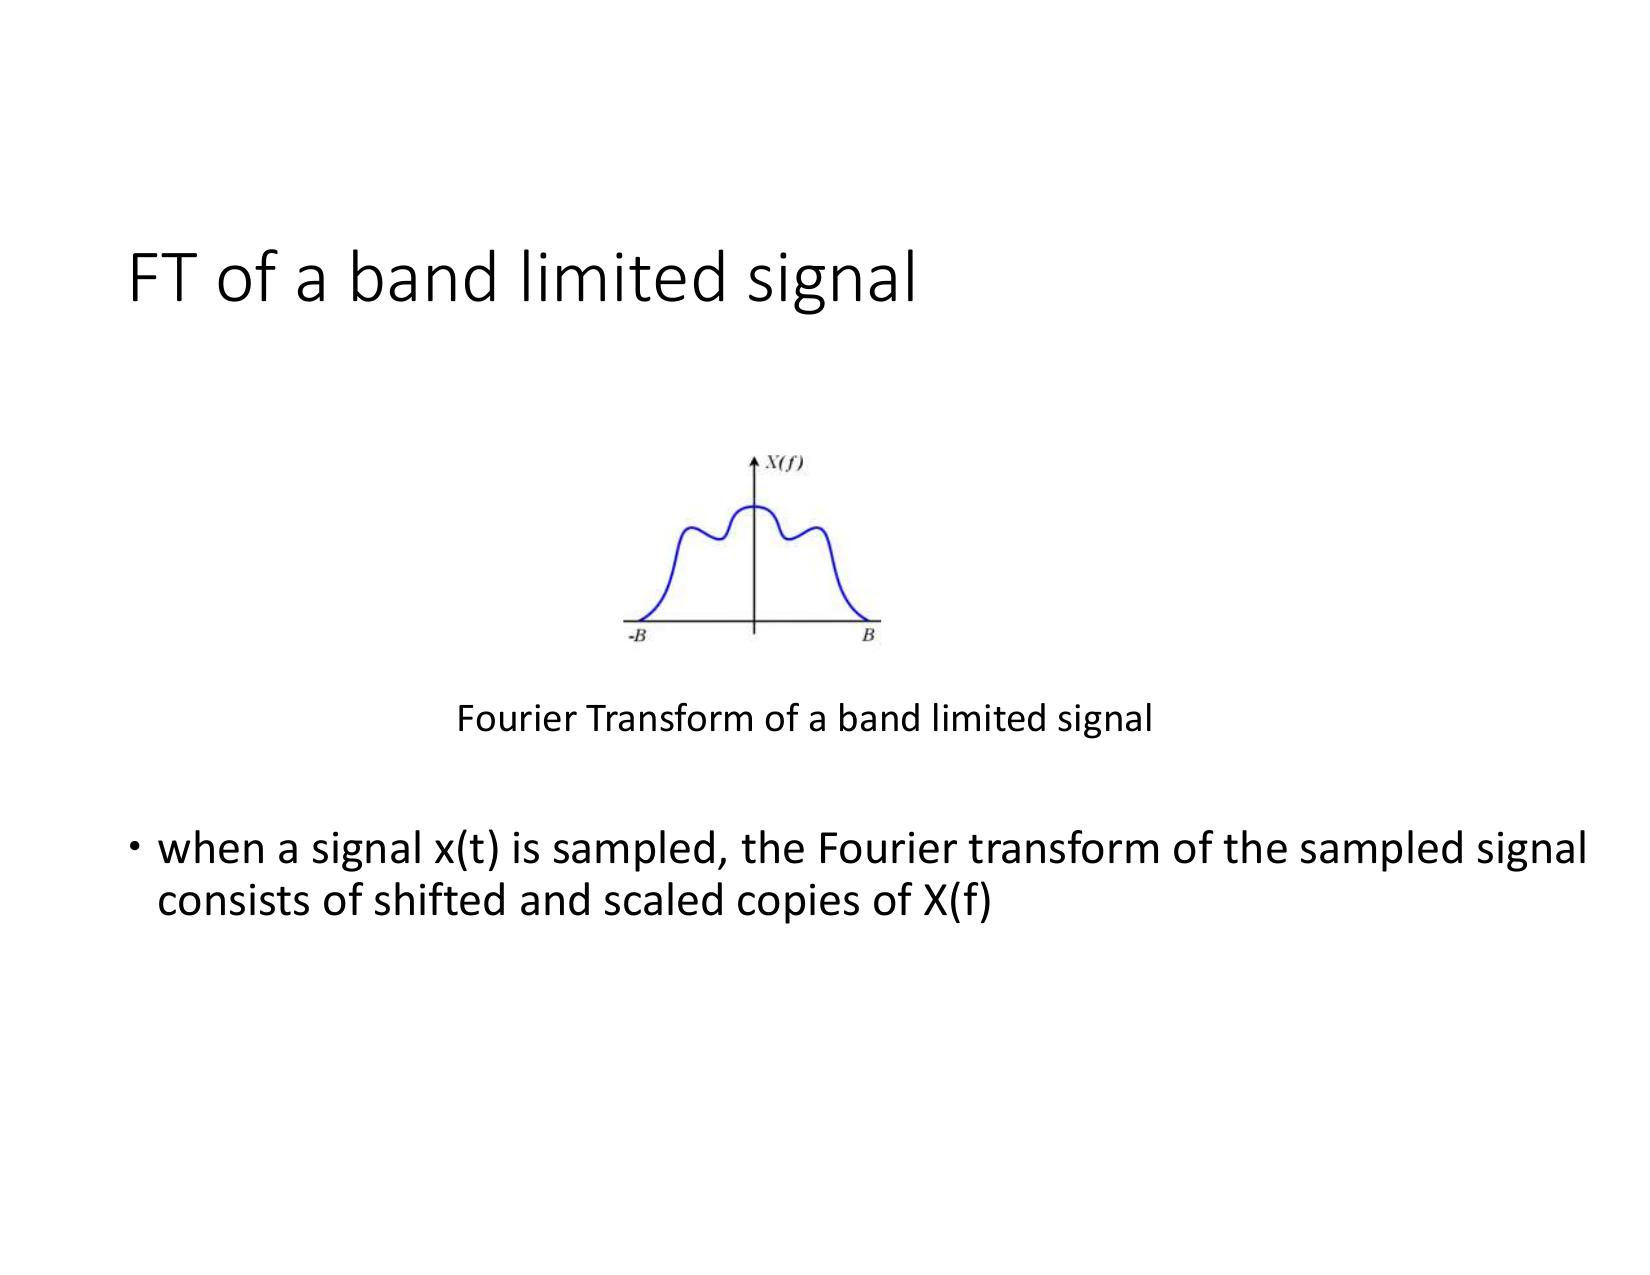
\includegraphics[keepaspectratio]{images/lezione-27-lab-teoria-dei-segnali-trasformata-di-fourier-campionamento-e-dft-img-08.jpg}}
\caption{Trasformata di Fourier di un segnale a banda limitata B. Quando
il segnale viene campionato, lo spettro si ``replica'' attorno a
multipli della frequenza di campionamento fs.}
\end{figure}

\begin{figure}
\centering
\pandocbounded{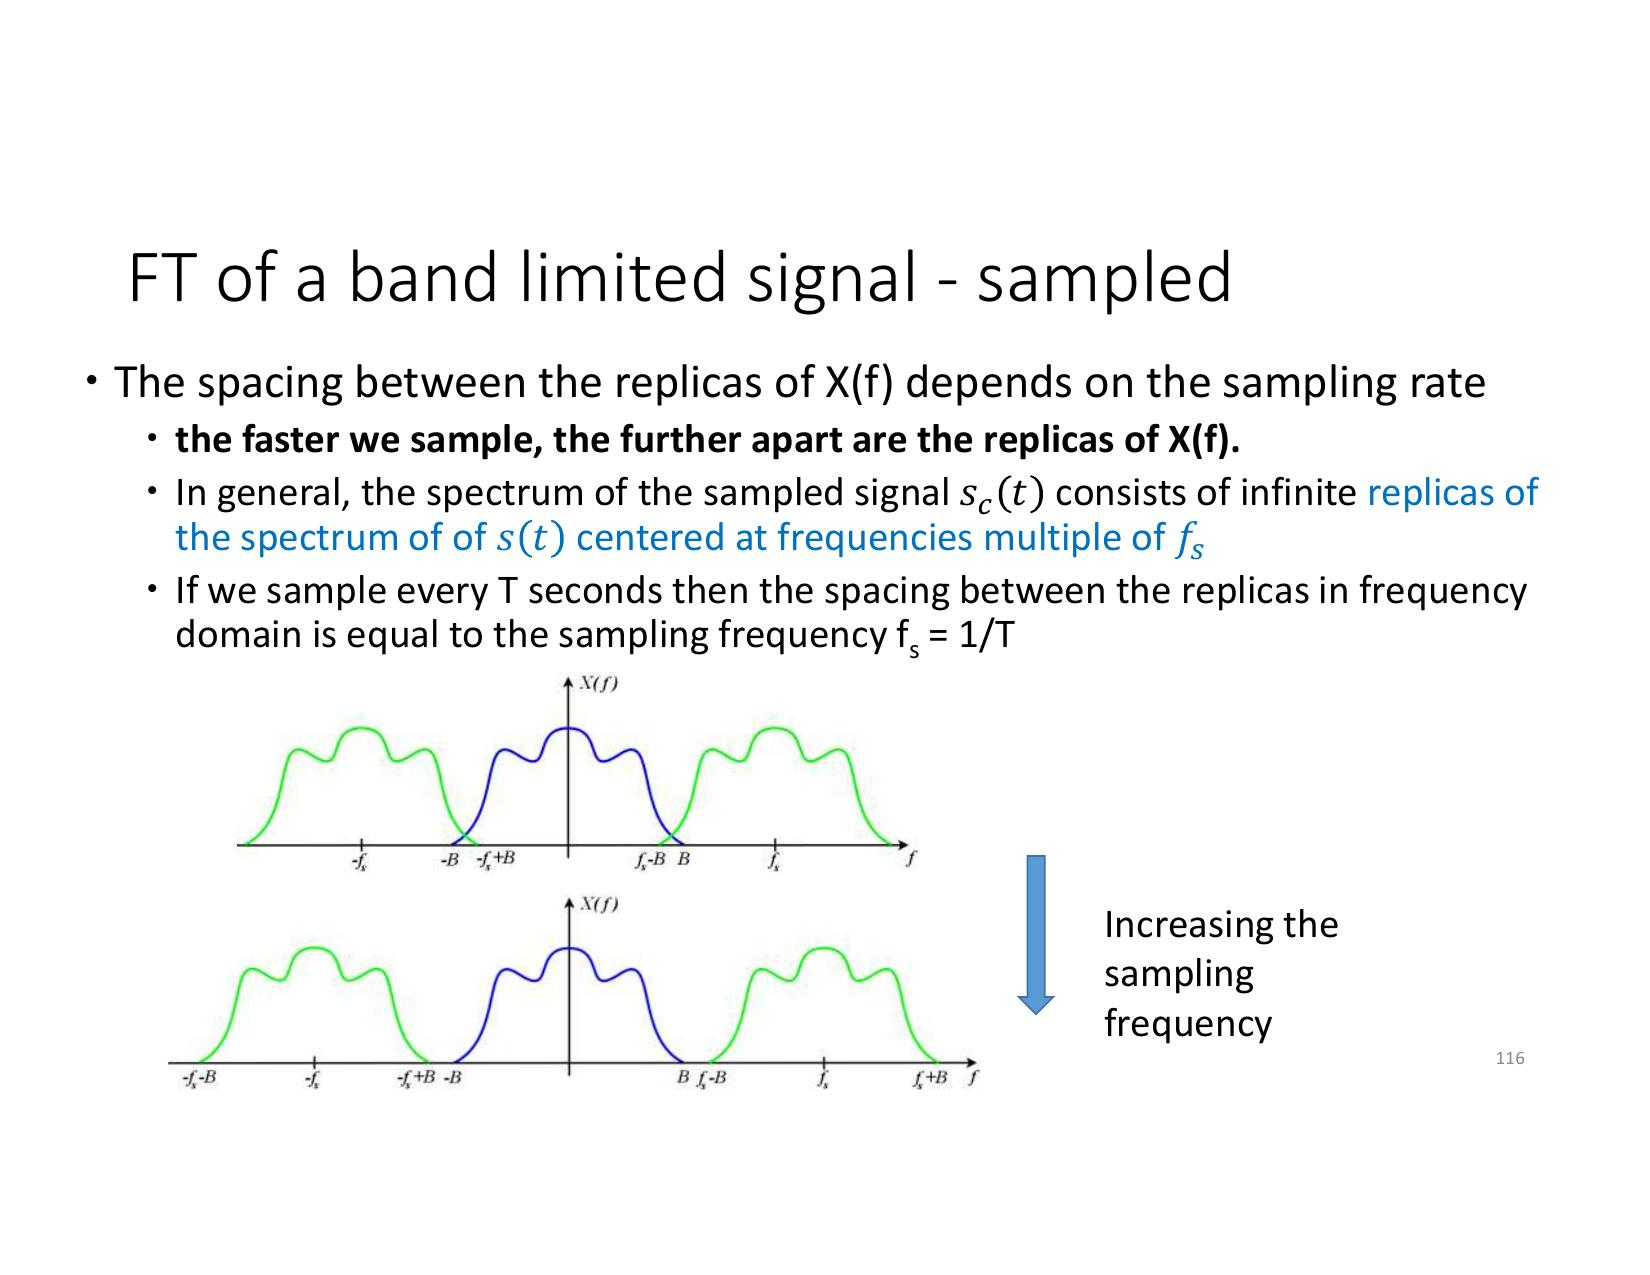
\includegraphics[keepaspectratio]{images/lezione-27-lab-teoria-dei-segnali-trasformata-di-fourier-campionamento-e-dft-img-09.jpg}}
\caption{Aumentando la frequenza di campionamento, le repliche dello
spettro si allontanano. Con campionamento sufficientemente veloce (in
basso), le repliche non si sovrappongono e il segnale originale è
recuperabile applicando un filtro passa-basso.}
\end{figure}

\begin{calloutdefinition}{Aliasing}

L'\textbf{aliasing} è la distorsione che si verifica quando le repliche
spettrali generate dal campionamento si \textbf{sovrappongono} tra loro.
Quando c'è sovrapposizione, le componenti frequenziali si mescolano e il
segnale originale non può più essere ricostruito univocamente.

\end{calloutdefinition}

\begin{figure}
\centering
\pandocbounded{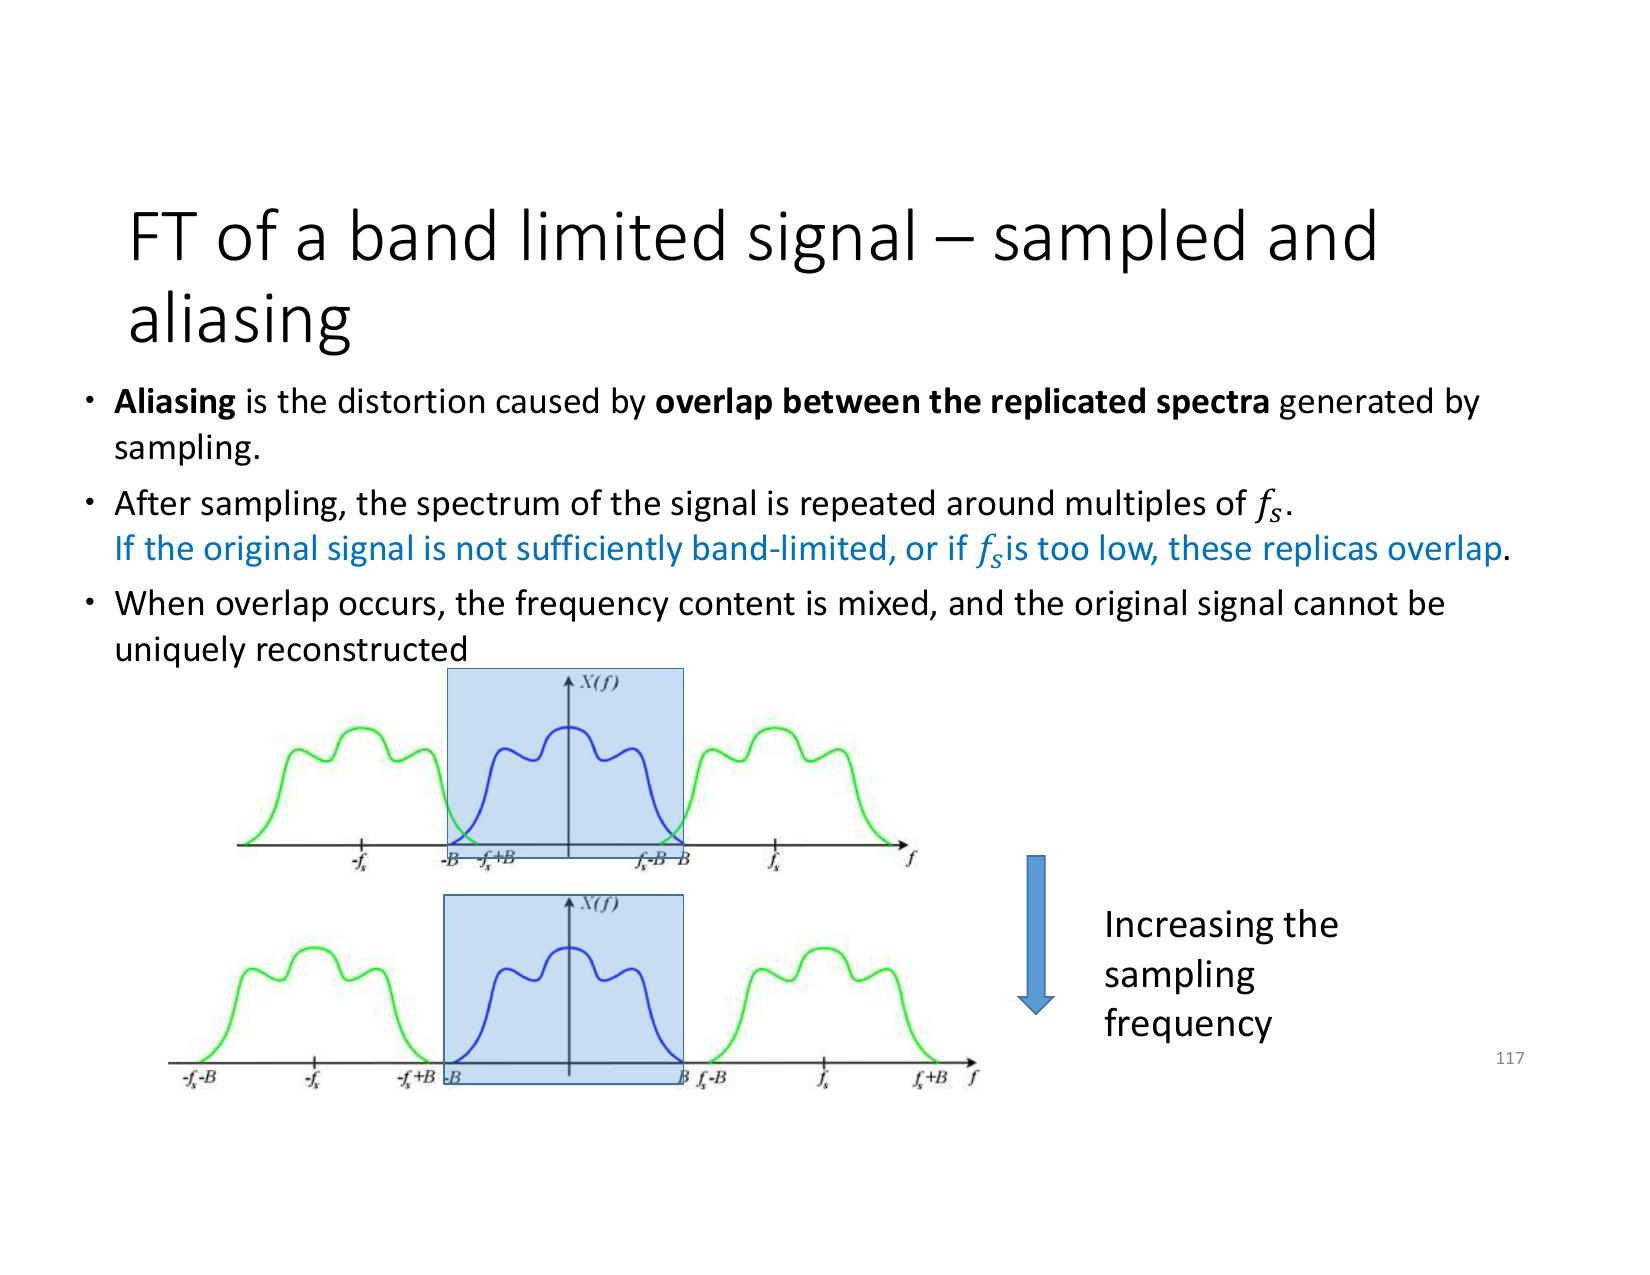
\includegraphics[keepaspectratio]{images/lezione-27-lab-teoria-dei-segnali-trasformata-di-fourier-campionamento-e-dft-img-10.jpg}}
\caption{Aliasing per frequenza di campionamento insufficiente: la
spaziatura tra repliche è minore di 2B e le code degli spettri si
sovrappongono, rendendo impossibile la ricostruzione.}
\end{figure}

La condizione di Nyquist garantisce che \textbf{non ci sia
sovrapposizione}: se \(f_s \geq 2f_M\), le repliche distano almeno
\(2B\) e possono essere separate con un filtro passa-basso ideale.

\begin{figure}
\centering
\pandocbounded{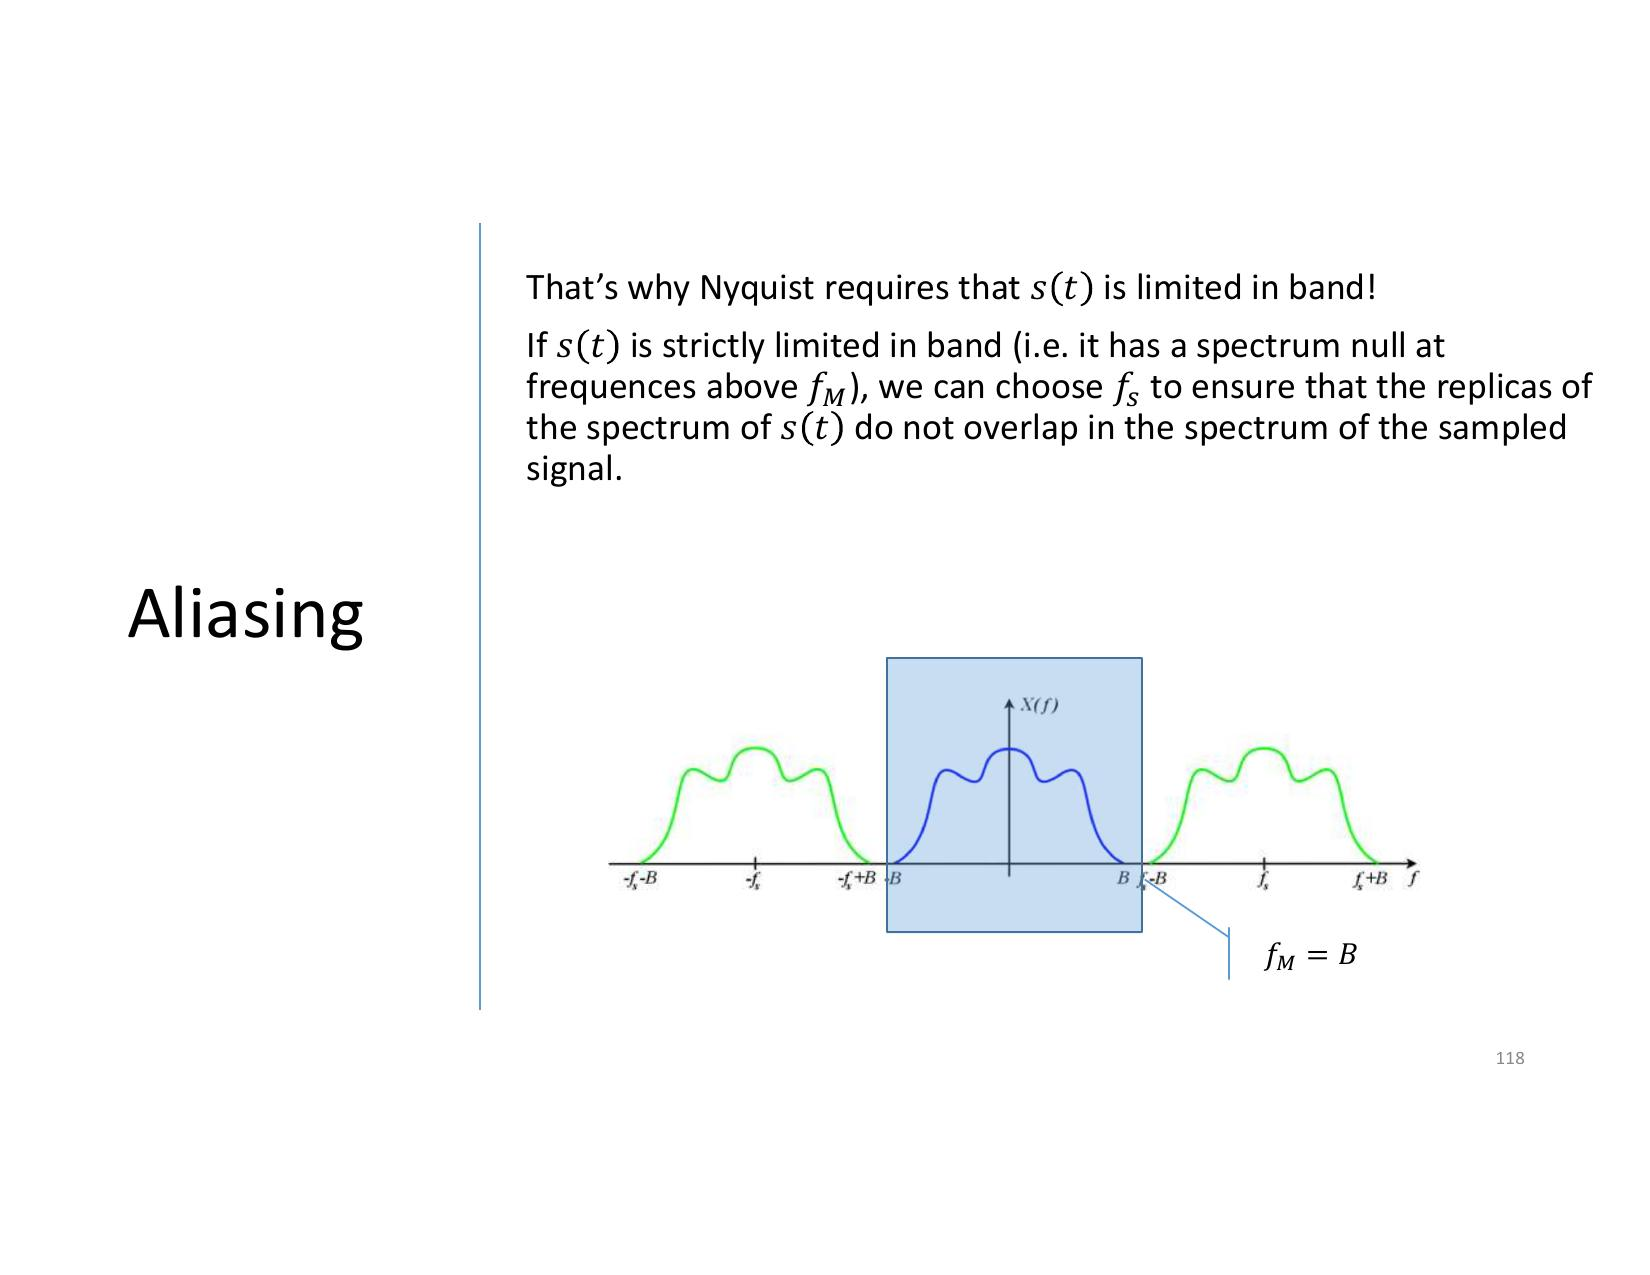
\includegraphics[keepaspectratio]{images/lezione-27-lab-teoria-dei-segnali-trasformata-di-fourier-campionamento-e-dft-img-11.jpg}}
\caption{Quando la condizione di Nyquist è soddisfatta (fs = 2B = 2fM),
le repliche dello spettro si toccano esattamente senza sovrapporsi: il
segnale originale è recuperabile con un filtro ideale.}
\end{figure}

\subsection{Cosa Nyquist Non Ha Detto}\label{cosa-nyquist-non-ha-detto}

Il teorema di Nyquist è spesso mal interpretato nella pratica. Ecco le
trappole più comuni:

\begin{calloutwarning}{Limiti pratici del teorema di Nyquist}

\begin{enumerate}
\def\labelenumi{\arabic{enumi}.}
\item
  \textbf{Nessun segnale reale è strettamente a banda limitata.} Un
  segnale a banda strettamente limitata deve estendersi infinitamente
  nel tempo, il che è fisicamente impossibile. In pratica, i segnali
  hanno uno spettro che decade ma non si azzera mai.
\item
  \textbf{Campionare a \(2f_M\) non basta se non si usa un filtro
  anti-aliasing perfetto.} I filtri reali non hanno una risposta
  rettangolare ideale: frequenze superiori a \(f_M\) passano, seppur
  attenuate. Il risultato è un aliasing residuo non trascurabile.
\item
  \textbf{La soluzione pratica è l'oversampling}: campionare a una
  frequenza significativamente superiore a \(2f_M\), e applicare un
  filtro anti-aliasing con taglio a \(f_M\) (anche se non ideale,
  l'attenuazione supplementare è sufficiente).
\end{enumerate}

\end{calloutwarning}

\begin{callouttip}{Oversampling nel telefono (old analog)}

Il telefono analogico tradizionale tagliava la voce a \textasciitilde3
kHz (non 4 kHz) e campionava a 8 kHz: non il doppio del taglio (che
sarebbe 6 kHz), ma un oversampling moderato. La differenza copre
l'imperfezione del filtro e le componenti residue tra 3 e 4 kHz.

\end{callouttip}

\begin{calloutnote}{Downsampling e segnali periodici}

Una curiosità: per segnali \textbf{strettamente periodici} e stabili, si
può addirittura \emph{sottocampionare} (\(f_s < 2f_M\)). Ogni campione
cade in una fase diversa del ciclo (perché il periodo di campionamento
non è un multiplo del periodo del segnale). Raccogliendo abbastanza
campioni nel tempo, si coprono tutte le fasi del segnale e la
ricostruzione diventa possibile. Questo funziona \textbf{solo} se il
segnale non varia nel tempo.

\end{calloutnote}

\begin{center}\rule{0.5\linewidth}{0.5pt}\end{center}

\section{Trasformata Discreta di Fourier
(DFT)}\label{trasformata-discreta-di-fourier-dft}

Nel contesto del \textbf{digital signal processing}, né la serie di
Fourier (richiede un segnale periodico continuo) né la CFT (richiede
un'integrazione continua) sono direttamente applicabili: si ha sempre un
numero finito di campioni. La \textbf{DFT} è lo strumento adatto.

\subsection{Motivazione}\label{motivazione}

Data una sequenza finita di \(N\) campioni \(s_k\) (con
\(k = 0, 1, \ldots, N-1\)), ottenuta campionando un segnale a frequenza
\(f_s\) per un tempo \(T = N/f_s\), si tratta il segnale discreto come
se fosse \textbf{periodico con periodo \(T\)} e si calcola la serie di
Fourier corrispondente. I coefficienti risultanti formano la DFT.

\subsection{Definizione della DFT}\label{definizione-della-dft}

\begin{calloutdefinition}{Trasformata Discreta di Fourier (DFT)}

Data una sequenza \(s_k\) di \(N\) valori (\(k = 0, 1, \ldots, N-1\)):

\textbf{Trasformata diretta:}
\[S_n = \sum_{k=0}^{N-1} s_k \, e^{-j2\pi nk/N}, \quad n = 0, 1, \ldots, N-1\]

\textbf{Trasformata inversa:}
\[s_k = \frac{1}{N} \sum_{n=0}^{N-1} S_n \, e^{j2\pi nk/N}\]

La frequenza del bin \(n\)-esimo è \(f_n = n \cdot \Delta f\), dove la
\textbf{risoluzione in frequenza} è:
\[\Delta f = \frac{f_s}{N} = \frac{1}{T}\]

\end{calloutdefinition}

La DFT prende in input un array di \(N\) valori e restituisce un array
di \(N\) valori complessi: entrambe le operazioni sono \textbf{somme}
(non integrali), quindi direttamente implementabili su un computer.

\begin{callouttip}{Esempio DFT}

Sequenza di 8 campioni: \(s[n] = 1\) per \(n = 0,1,2,3\) e \(s[n] = 0\)
per \(n = 4,5,6,7\).

I coefficienti DFT risultano: - \(S_0 = 4\) (componente DC) -
\(S_1 = 1 - j2.414\) - \(S_2 = 1 - j0.414\)\\
- \(S_3 = 1 + j0.414\) - \(S_4 = 1 + j2.414\) - \(S_5 = S_6 = S_7 = 0\)
(per parità)

\end{callouttip}

\begin{figure}
\centering
\pandocbounded{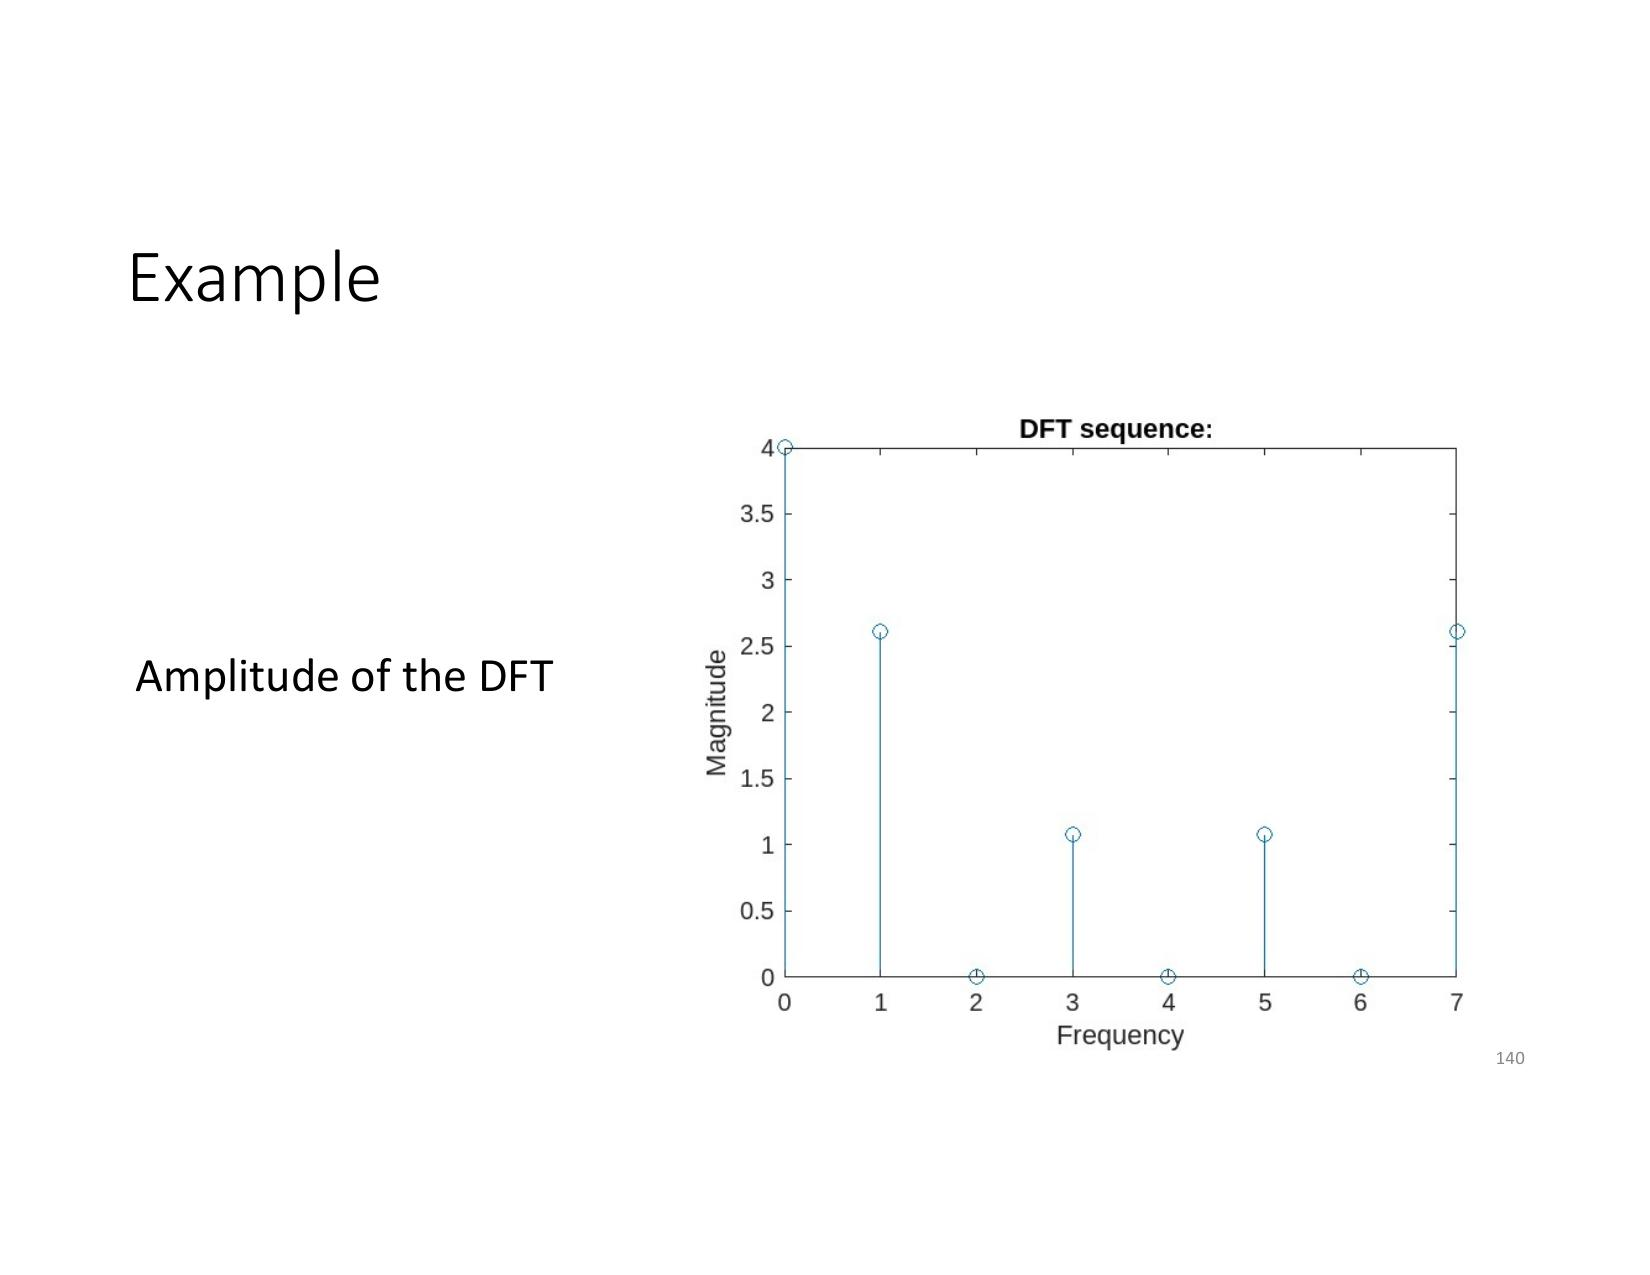
\includegraphics[keepaspectratio]{images/lezione-27-lab-teoria-dei-segnali-trasformata-di-fourier-campionamento-e-dft-img-12.jpg}}
\caption{Spettro di ampiezza \textbar S\_n\textbar{} della DFT
dell'esempio. Il valore DC (n=0) vale 4, poi i bin hanno ampiezze che
decrescono. La simmetria attorno a N/2 è caratteristica della DFT di
segnali reali.}
\end{figure}

\subsection{Fast Fourier Transform
(FFT)}\label{fast-fourier-transform-fft}

Il calcolo diretto della DFT richiede \(O(N^2)\) operazioni. Per
sequenze lunghe (audio HD: \(N = 44100\) o più), questo è proibitivo. La
\textbf{FFT} (Fast Fourier Transform) è una famiglia di algoritmi che
sfruttano la struttura periodica dell'esponenziale complesso per ridurre
la complessità a \(O(N \log N)\).

\begin{calloutnote}{Condizione sulla lunghezza}

Per la FFT più efficiente (algoritmo di Cooley-Tukey), \(N\) deve essere
una potenza di 2: \(N = 2^k\). Per questo le frequenze di campionamento
standard come 44100 Hz vengono spesso arrotondate a \(N = 32768\) o
\(65536\) campioni per la trasformazione.

\end{calloutnote}

\subsection{Commenti sulla DFT}\label{commenti-sulla-dft}

\textbf{Risoluzione in frequenza.} La DFT non ha una risoluzione
arbitraria: i ``bin'' sono spaziati di \(\Delta f = f_s / N\). Se una
componente del segnale cade tra due bin, la sua energia si spalma su più
bin adiacenti (\textbf{spectral leakage}). Per migliorare la risoluzione
si deve aumentare \(N\) (osservare il segnale più a lungo).

\textbf{Frequenza di Nyquist nella DFT.} L'analisi spettrale affidabile
tramite DFT è possibile solo per frequenze \(f < f_s/2\): le componenti
oltre la frequenza di Nyquist vengono mappate a frequenze errate
(aliasing). Filtri anti-aliasing vengono applicati prima del
campionamento per rimuovere le componenti fuori banda.

\begin{center}\rule{0.5\linewidth}{0.5pt}\end{center}

\begin{calloutnote}{Riepilogo dei domini di Fourier}

{\def\LTcaptype{none} % do not increment counter
\begin{longtable}[]{@{}
  >{\raggedright\arraybackslash}p{(\linewidth - 6\tabcolsep) * \real{0.2500}}
  >{\raggedright\arraybackslash}p{(\linewidth - 6\tabcolsep) * \real{0.2500}}
  >{\raggedright\arraybackslash}p{(\linewidth - 6\tabcolsep) * \real{0.2500}}
  >{\raggedright\arraybackslash}p{(\linewidth - 6\tabcolsep) * \real{0.2500}}@{}}
\toprule\noalign{}
\begin{minipage}[b]{\linewidth}\raggedright
Strumento
\end{minipage} & \begin{minipage}[b]{\linewidth}\raggedright
Tipo di segnale
\end{minipage} & \begin{minipage}[b]{\linewidth}\raggedright
Tipo di spettro
\end{minipage} & \begin{minipage}[b]{\linewidth}\raggedright
Operatori
\end{minipage} \\
\midrule\noalign{}
\endhead
\bottomrule\noalign{}
\endlastfoot
\textbf{Serie di Fourier} & Periodico continuo & Discreto (coefficienti
\(S_n\)) & Integrale → Somma \\
\textbf{CFT} & Non periodico continuo & Continuo \(S(f)\) & Integrale →
Integrale \\
\textbf{DFT} & Discreto (N campioni) & Discreto (N coefficienti) & Somma
→ Somma \\
\end{longtable}
}

La DFT può essere vista come la serie di Fourier del segnale campionato,
trattato come periodico con periodo \(T = N/f_s\).

\end{calloutnote}

\begin{center}\rule{0.5\linewidth}{0.5pt}\end{center}

\begin{calloutquestion}{Possibili domande d’esame}

\begin{itemize}
\tightlist
\item
  Quali sono le quattro classi di segnali secondo la classificazione
  tempo/ampiezza? Fai esempi.
\item
  Cos'è il bitrate di una sorgente digitale? Come dipende da frequenza
  di campionamento e bit per campione?
\item
  Enuncia il teorema di Shannon sulla capacità di canale. Come lega SNR,
  banda e bitrate?
\item
  Cos'è la serie di Fourier? Scrivi la formula generale e i coefficienti
  \(a_0\), \(a_n\), \(b_n\).
\item
  Quali sono le condizioni sufficienti di Dirichlet per l'esistenza
  della serie di Fourier?
\item
  Cos'è il fenomeno di Gibbs? Perché non scompare aggiungendo più
  armoniche?
\item
  Come si passa dalla serie di Fourier reale a quella in forma
  esponenziale complessa?
\item
  Cos'è lo spettro di un segnale? Perché si rappresentano due diagrammi
  separati (ampiezza e fase)?
\item
  Perché la serie di Fourier di un segnale aperiodico produce la sua
  estensione periodica?
\item
  Calcola i coefficienti della serie di Fourier per un'onda quadra
  semplice (es. \(s(t) = 1\) per \(0 < t < T/2\), \(s(t) = -1\) per
  \(T/2 < t < T\)).
\item
  Qual è la differenza concettuale tra serie di Fourier e trasformata di
  Fourier?
\item
  Perché campionare un segnale genera repliche spettrali? Cosa succede
  se le repliche si sovrappongono?
\item
  Enunciare il teorema di Nyquist-Shannon. Quali sono le sue ipotesi e i
  suoi limiti pratici?
\item
  Cosa si intende per aliasing? Come si previene?
\item
  Cosa si intende per risoluzione della DFT? Come si può migliorarla?
\item
  Qual è la complessità computazionale della DFT e della FFT?
\item
  Perché nessun segnale reale è strettamente a banda limitata? Quali
  conseguenze ha questo per il campionamento?
\end{itemize}

\end{calloutquestion}

\newpage

\chapter{03 - Reti Mobili: Architettura e Mobilità dal 4G al
5G}\label{reti-mobili-architettura-e-mobilituxe0-dal-4g-al-5g}

Questa lezione introduce i fondamenti dell'architettura delle reti
cellulari moderne, ripercorrendo l'evoluzione storica dal 1G fino al 5G
e proiettandosi verso il 6G. Analizza come ogni generazione abbia
trasformato il modello architetturale fino ad arrivare
all'\textbf{all-IP core} del 4G LTE e alla \textbf{Service Based
Architecture} del 5G. Esamineremo inoltre i meccanismi che rendono la
mobilità un servizio nativo di prima classe, il tunneling GTP per il
routing indiretto, l'autenticazione mutua (AKA) basata su SIM, e la
separazione fra piano di controllo e piano dati.

\begin{calloutnote}{Riferimenti bibliografici}

Le slide sono un libero adattamento del libro \textbf{``Computer
Networking: A Top-Down Approach''} (8ª edizione, 2020) di James F.
Kurose e Keith W. Ross. Per l'architettura 5G il riferimento è
\textbf{``5G Mobile Networks: A Systems Approach''} di Larry Peterson e
Oguz Sunay. Il quadro evolutivo verso il 6G riprende: Zakria Qadir et
al., \emph{``Towards 6G Internet of Things: Recent advances, use cases,
and open challenges''}, Elsevier, Giugno 2023.

\end{calloutnote}

\begin{center}\rule{0.5\linewidth}{0.5pt}\end{center}

\section{L'evoluzione delle reti cellulari: dal 1G al
6G}\label{levoluzione-delle-reti-cellulari-dal-1g-al-6g}

Le reti cellulari hanno attraversato una trasformazione da semplici
sistemi di telefonia analogica a infrastrutture distribuite per
l'Internet of Things globale.

Il \textbf{1G} degli anni '80 (AMPS, TACS) trasportava voce analogica
multiplexata in frequenza (FDMA). Negli anni '90 il \textbf{2G}
introduce voce digitale (GSM, CDMA) con TDM+FDM e SMS; con l'estensione
\textbf{2.5G/GPRS} si affaccia la \textbf{commutazione a pacchetto per i
dati}. Il \textbf{3G} (UMTS, HSPDA) porta l'accesso Web in mobilità:
voce a circuito, dati a pacchetto.

La svolta architetturale arriva con il \textbf{4G} (LTE Advanced): tutto
il traffico viaggia su un \textbf{All-IP core}, tunnelizzato come
pacchetti IP dalla Base Station al gateway. Si introduce la separazione
fra piano di controllo e piano dati. Il \textbf{5G} (5G NR) ridisegna il
core in chiave cloud-native (\textbf{Service Based Architecture}),
introduce il \textbf{network slicing} e sfrutta frequenze sub-6 GHz e
onde millimetriche (mmWave). Il \textbf{6G}, atteso intorno al 2030,
punta a un ecosistema ``fully-connected'' potenziato da AI con
architetture \emph{cell-less}.

{\def\LTcaptype{none} % do not increment counter
\begin{longtable}[]{@{}
  >{\raggedright\arraybackslash}p{(\linewidth - 14\tabcolsep) * \real{0.1250}}
  >{\raggedright\arraybackslash}p{(\linewidth - 14\tabcolsep) * \real{0.1250}}
  >{\raggedright\arraybackslash}p{(\linewidth - 14\tabcolsep) * \real{0.1250}}
  >{\raggedright\arraybackslash}p{(\linewidth - 14\tabcolsep) * \real{0.1250}}
  >{\raggedright\arraybackslash}p{(\linewidth - 14\tabcolsep) * \real{0.1250}}
  >{\raggedright\arraybackslash}p{(\linewidth - 14\tabcolsep) * \real{0.1250}}
  >{\raggedright\arraybackslash}p{(\linewidth - 14\tabcolsep) * \real{0.1250}}
  >{\raggedright\arraybackslash}p{(\linewidth - 14\tabcolsep) * \real{0.1250}}@{}}
\toprule\noalign{}
\begin{minipage}[b]{\linewidth}\raggedright
Gen
\end{minipage} & \begin{minipage}[b]{\linewidth}\raggedright
Anni
\end{minipage} & \begin{minipage}[b]{\linewidth}\raggedright
Standard
\end{minipage} & \begin{minipage}[b]{\linewidth}\raggedright
Velocità
\end{minipage} & \begin{minipage}[b]{\linewidth}\raggedright
Accesso
\end{minipage} & \begin{minipage}[b]{\linewidth}\raggedright
Voice switch
\end{minipage} & \begin{minipage}[b]{\linewidth}\raggedright
Data switch
\end{minipage} & \begin{minipage}[b]{\linewidth}\raggedright
Caratteristiche
\end{minipage} \\
\midrule\noalign{}
\endhead
\bottomrule\noalign{}
\endlastfoot
\textbf{1G} & 1980s & AMPS, TACS & 2.4 kbps & FDMA & Circuit & Circuit &
Voce analogica, copertura limitata \\
\textbf{2G} & 1990s & GSM, CDMA, EDGE & 64 kbps & TDM+FDM & Circuit &
Circuit & Voce digitale + SMS \\
\textbf{2.5G} & fine '90s & GPRS & --- & --- & Circuit & Packet & Prima
commutazione a pacchetto sui dati \\
\textbf{3G} & 2000s & UMTS, HSPDA & fino a 2 Mbps & CDMA & Circuit &
Packet & Web in mobilità \\
\textbf{4G} & 2010s & LTE Advanced & 100--1000 Mbps & OFDMA & Packet &
Packet & All-IP core, tunneling, separazione control/data \\
\textbf{5G} & 2020s & 5G NR & fino a \textasciitilde20 Gbps & OFDMA +
mmWave & Packet & Packet & SBA, network slicing, sub-6 GHz + mmWave \\
\textbf{6G} & 2030s (prev.) & --- & \textasciitilde1 Tbps & --- & --- &
--- & Cell-less, AI-native, fully-connected \\
\end{longtable}
}

\begin{callouttip}{La traiettoria di fondo}

A ogni generazione la rete diventa più simile a Internet, modularizzando
il core in microservizi (5G). La direzione è una rete cellulare
\textbf{indistinguibile da un cloud distribuito}, dove la mobilità è una
feature applicativa.

\end{callouttip}

\begin{center}\rule{0.5\linewidth}{0.5pt}\end{center}

\section{Architettura di alto livello: RAN, Backhaul, Mobile
Core}\label{architettura-di-alto-livello-ran-backhaul-mobile-core}

L'architettura di una rete cellulare 4G/5G si scompone in tre blocchi
funzionali:

\begin{itemize}
\tightlist
\item
  \textbf{Radio Access Network (RAN)} --- la rete d'accesso radio: una
  collezione distribuita di \textbf{Base Station} che gestiscono lo
  spettro radio condiviso all'interno della loro \textbf{cella}.
\item
  \textbf{Backhaul Network} --- interconnette la RAN con il Mobile Core.
  Tipicamente in fibra ottica, o soluzioni wireless (IAB).
\item
  \textbf{Mobile Core Network} --- fornisce connettività IP per
  dati/voce, garantisce QoS, traccia la mobilità e gestisce billing.
  Chiamato \textbf{Evolved Packet Core (EPC)} in 4G e \textbf{NG-Core}
  in 5G.
\end{itemize}

\begin{figure}
\centering
\pandocbounded{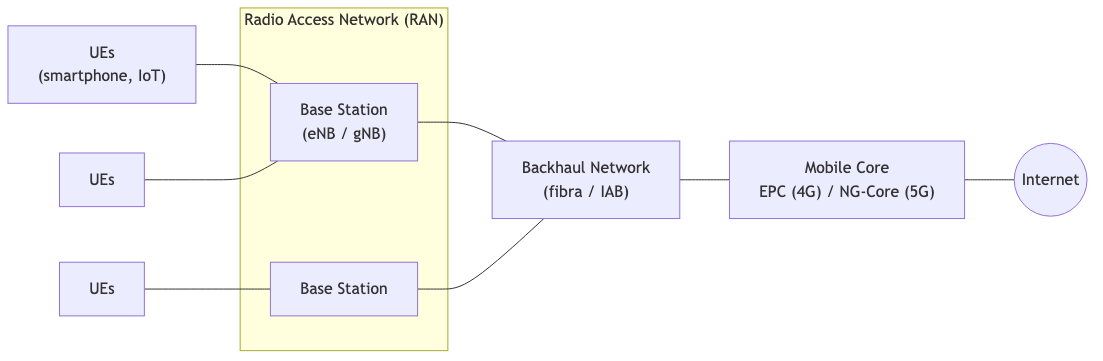
\includegraphics[keepaspectratio,alt={I tre blocchi dell'architettura cellulare. La RAN gestisce lo spettro radio per le comunicazioni con i dispositivi (UE), il backhaul trasporta il traffico verso il core, e il Mobile Core funge da gateway verso Internet gestendo mobilità e controllo.}]{images/mermaid-03-reti-mobili-tradizionali-01.png}}
\caption{I tre blocchi dell'architettura cellulare. La RAN gestisce lo
spettro radio per le comunicazioni con i dispositivi (UE), il backhaul
trasporta il traffico verso il core, e il Mobile Core funge da gateway
verso Internet gestendo mobilità e controllo.}
\end{figure}

\begin{center}\rule{0.5\linewidth}{0.5pt}\end{center}

\section{Gli elementi dell'architettura 4G
LTE}\label{gli-elementi-dellarchitettura-4g-lte}

L'architettura 4G LTE è chiamata \textbf{all-IP Enhanced Packet Core
(EPC)}. I concetti base sopravvivono in 5G:

\begin{itemize}
\tightlist
\item
  \textbf{User Equipment (UE)}: Qualsiasi dispositivo con radio LTE
  (smartphone, IoT). L'identità globale è l'\textbf{IMSI}, memorizzato
  sulla \textbf{SIM}.
\item
  \textbf{Base Station (eNode-B)}: Gestisce le risorse radio wireless
  nella sua cella. A differenza del Wi-Fi, coordina gli
  \textbf{handover}, minimizza interferenze, crea tunnel IP verso il
  core e gestisce la mobilità intercella.
\item
  \textbf{Mobility Management Entity (MME)}: ``Cervello'' del piano di
  controllo. Coordina l'autenticazione, handover, tracking/paging, e
  setup dei tunnel.
\item
  \textbf{Home Subscriber Service (HSS)}: Database centrale con info
  sugli abbonati. Collabora con MME per l'autenticazione.
\item
  \textbf{Serving Gateway (S-GW)}: Inoltra pacchetti dal/verso la RAN.
  Funge da \textbf{Local Mobility Anchor} durante gli handover
  inter-eNB.
\item
  \textbf{PDN Gateway (P-GW)}: Connette il core 4G alle reti dati
  esterne (Internet). Svolge NAT, policy, traffic shaping e charging.
  S-GW e P-GW possono essere co-locati.
\end{itemize}

\begin{figure}
\centering
\pandocbounded{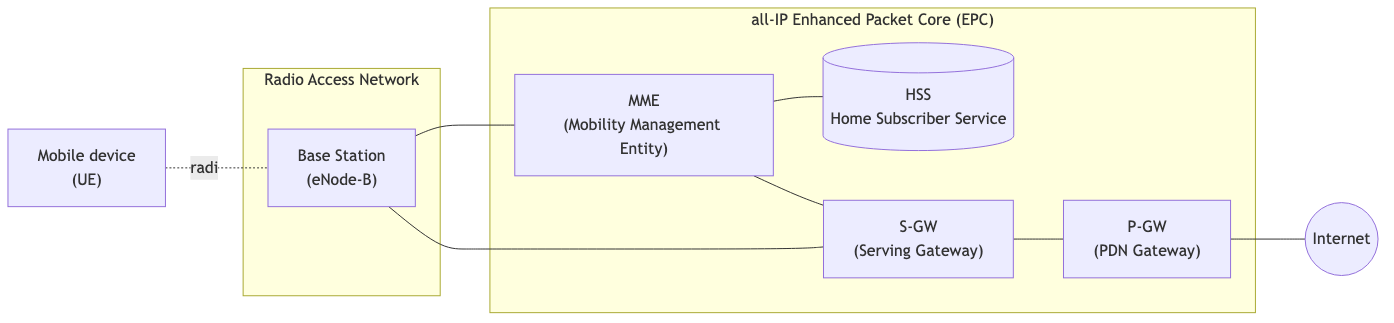
\includegraphics[keepaspectratio,alt={Topologia logica del 4G LTE. Le interfacce di controllo collegano la BS al MME e HSS, mentre il piano dati attraversa BS, S-GW e P-GW verso Internet.}]{images/mermaid-03-reti-mobili-tradizionali-02.png}}
\caption{Topologia logica del 4G LTE. Le interfacce di controllo
collegano la BS al MME e HSS, mentre il piano dati attraversa BS, S-GW e
P-GW verso Internet.}
\end{figure}

\subsection{Separazione tra Control Plane e Data
Plane}\label{separazione-tra-control-plane-e-data-plane}

L'LTE separa nettamente \textbf{Piano di Controllo} e \textbf{Piano
Dati}, principio mutuato dall'SDN. La Base Station si trova
sull'incrocio e inoltra entrambi. - \textbf{Control Plane}: pacchetti
tunnelizzati su \textbf{SCTP/IP} (protocollo affidabile per
segnalazione). - \textbf{Data Plane}: pacchetti incapsulati in tunnel
\textbf{GTP-U} (GPRS Tunneling Protocol over UDP).

\begin{figure}
\centering
\pandocbounded{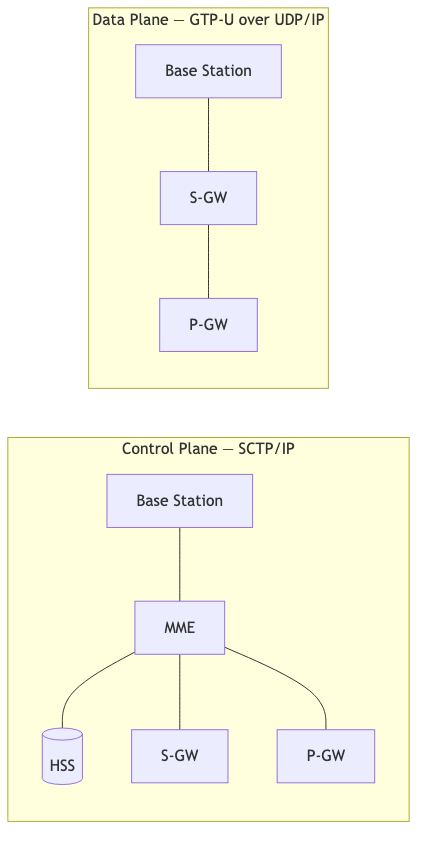
\includegraphics[keepaspectratio,alt={Separazione dei piani in LTE. Il Control Plane usa SCTP/IP per la segnalazione tra BS, MME, HSS e gateway. Il Data Plane usa tunnel GTP-U over UDP/IP per il traffico utente tra BS, S-GW e P-GW.}]{images/mermaid-03-reti-mobili-tradizionali-03.png}}
\caption{Separazione dei piani in LTE. Il Control Plane usa SCTP/IP per
la segnalazione tra BS, MME, HSS e gateway. Il Data Plane usa tunnel
GTP-U over UDP/IP per il traffico utente tra BS, S-GW e P-GW.}
\end{figure}

\begin{callouttip}{Perché la separazione è cruciale}

Disaccoppiare i piani permette di scalarli indipendentemente e abilita
la virtualizzazione delle funzioni di controllo (NFV), dominante nel 5G.

\end{callouttip}

\begin{center}\rule{0.5\linewidth}{0.5pt}\end{center}

\section{Lo Spettro della Mobilità e la Home
Network}\label{lo-spettro-della-mobilituxe0-e-la-home-network}

La mobilità non è una proprietà binaria. Per gestirla è indispensabile
una \textbf{home network}: una fonte autorevole che registra la
posizione del dispositivo. Nelle reti cellulari la home network è
l'operatore con cui l'utente ha il contratto (es. Vodafone, TIM), il cui
database è l'HSS. Quando un dispositivo lascia la propria rete, entra in
una \textbf{visited network} (\emph{roaming}), basato su accordi
commerciali.

\begin{figure}
\centering
\pandocbounded{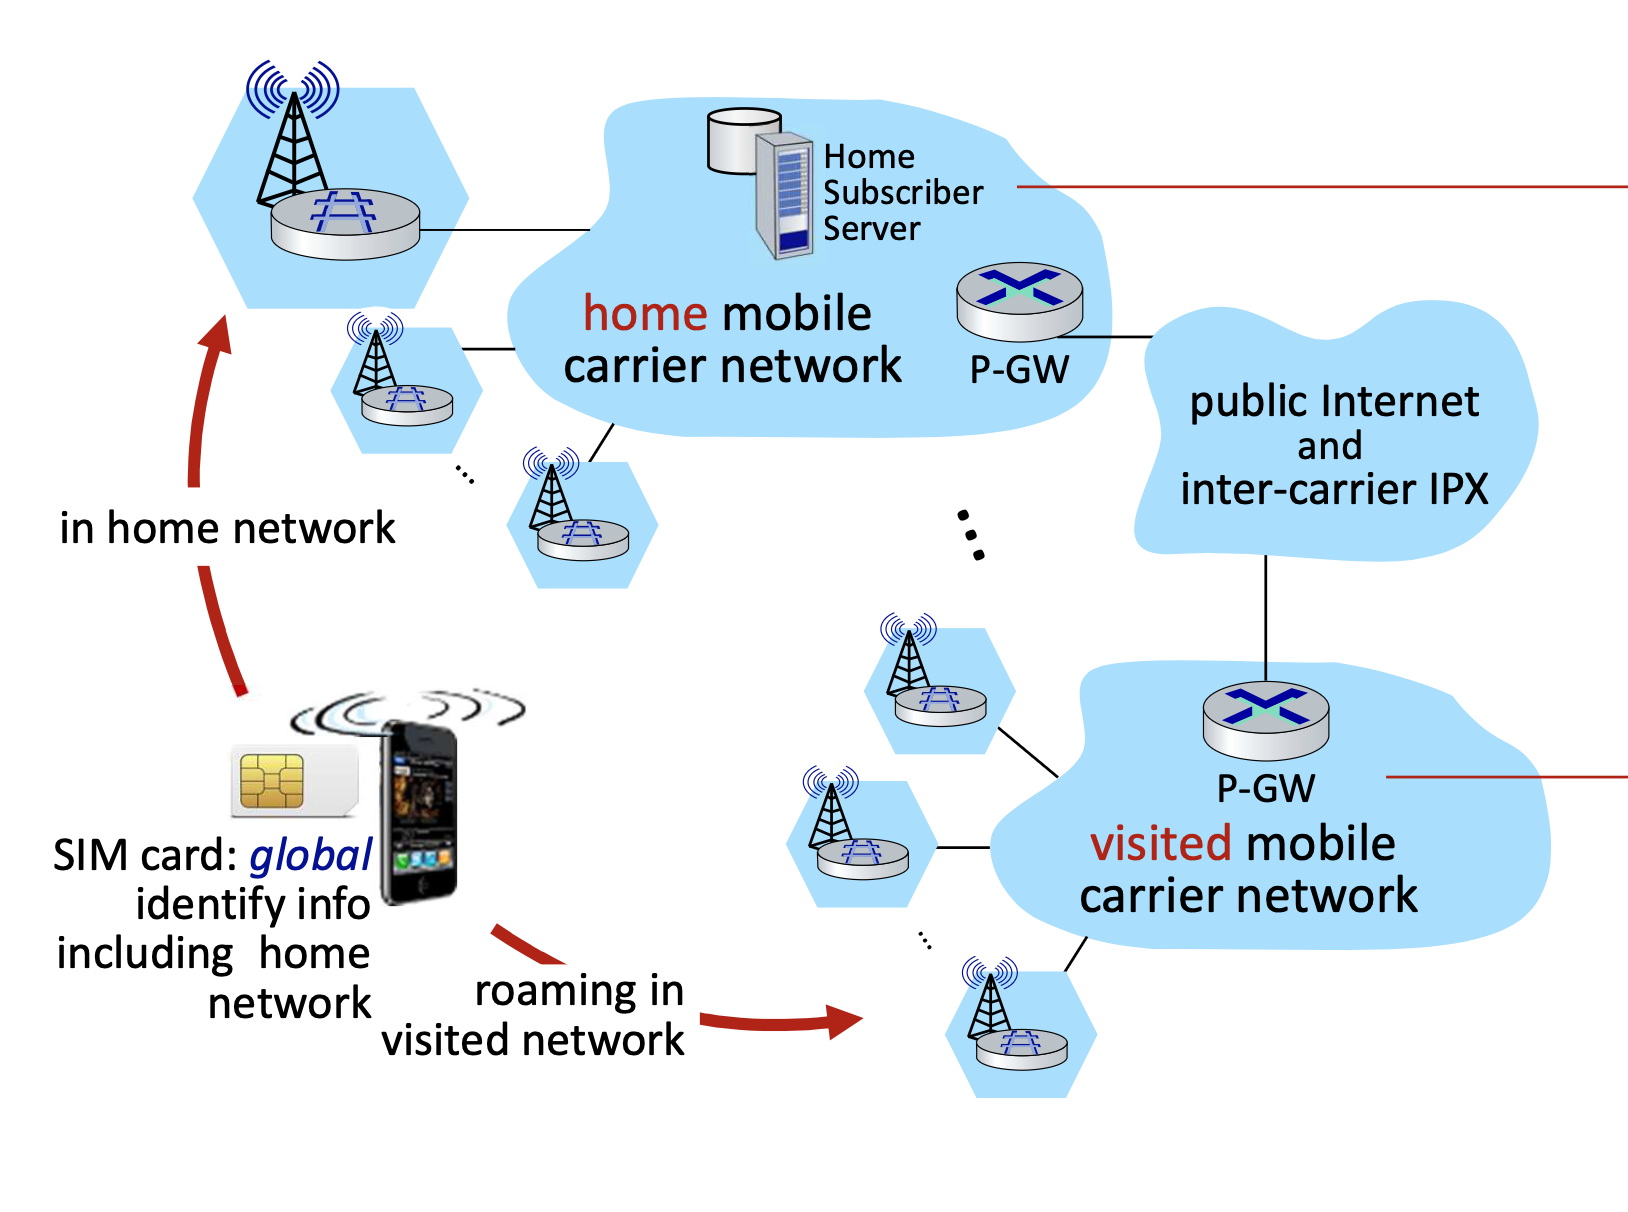
\includegraphics[keepaspectratio]{images/Screenshot-2026-03-10-alle-14-37-18.png}}
\caption{Struttura della home network in un'architettura 4G/5G.}
\end{figure}

\begin{figure}
\centering
\pandocbounded{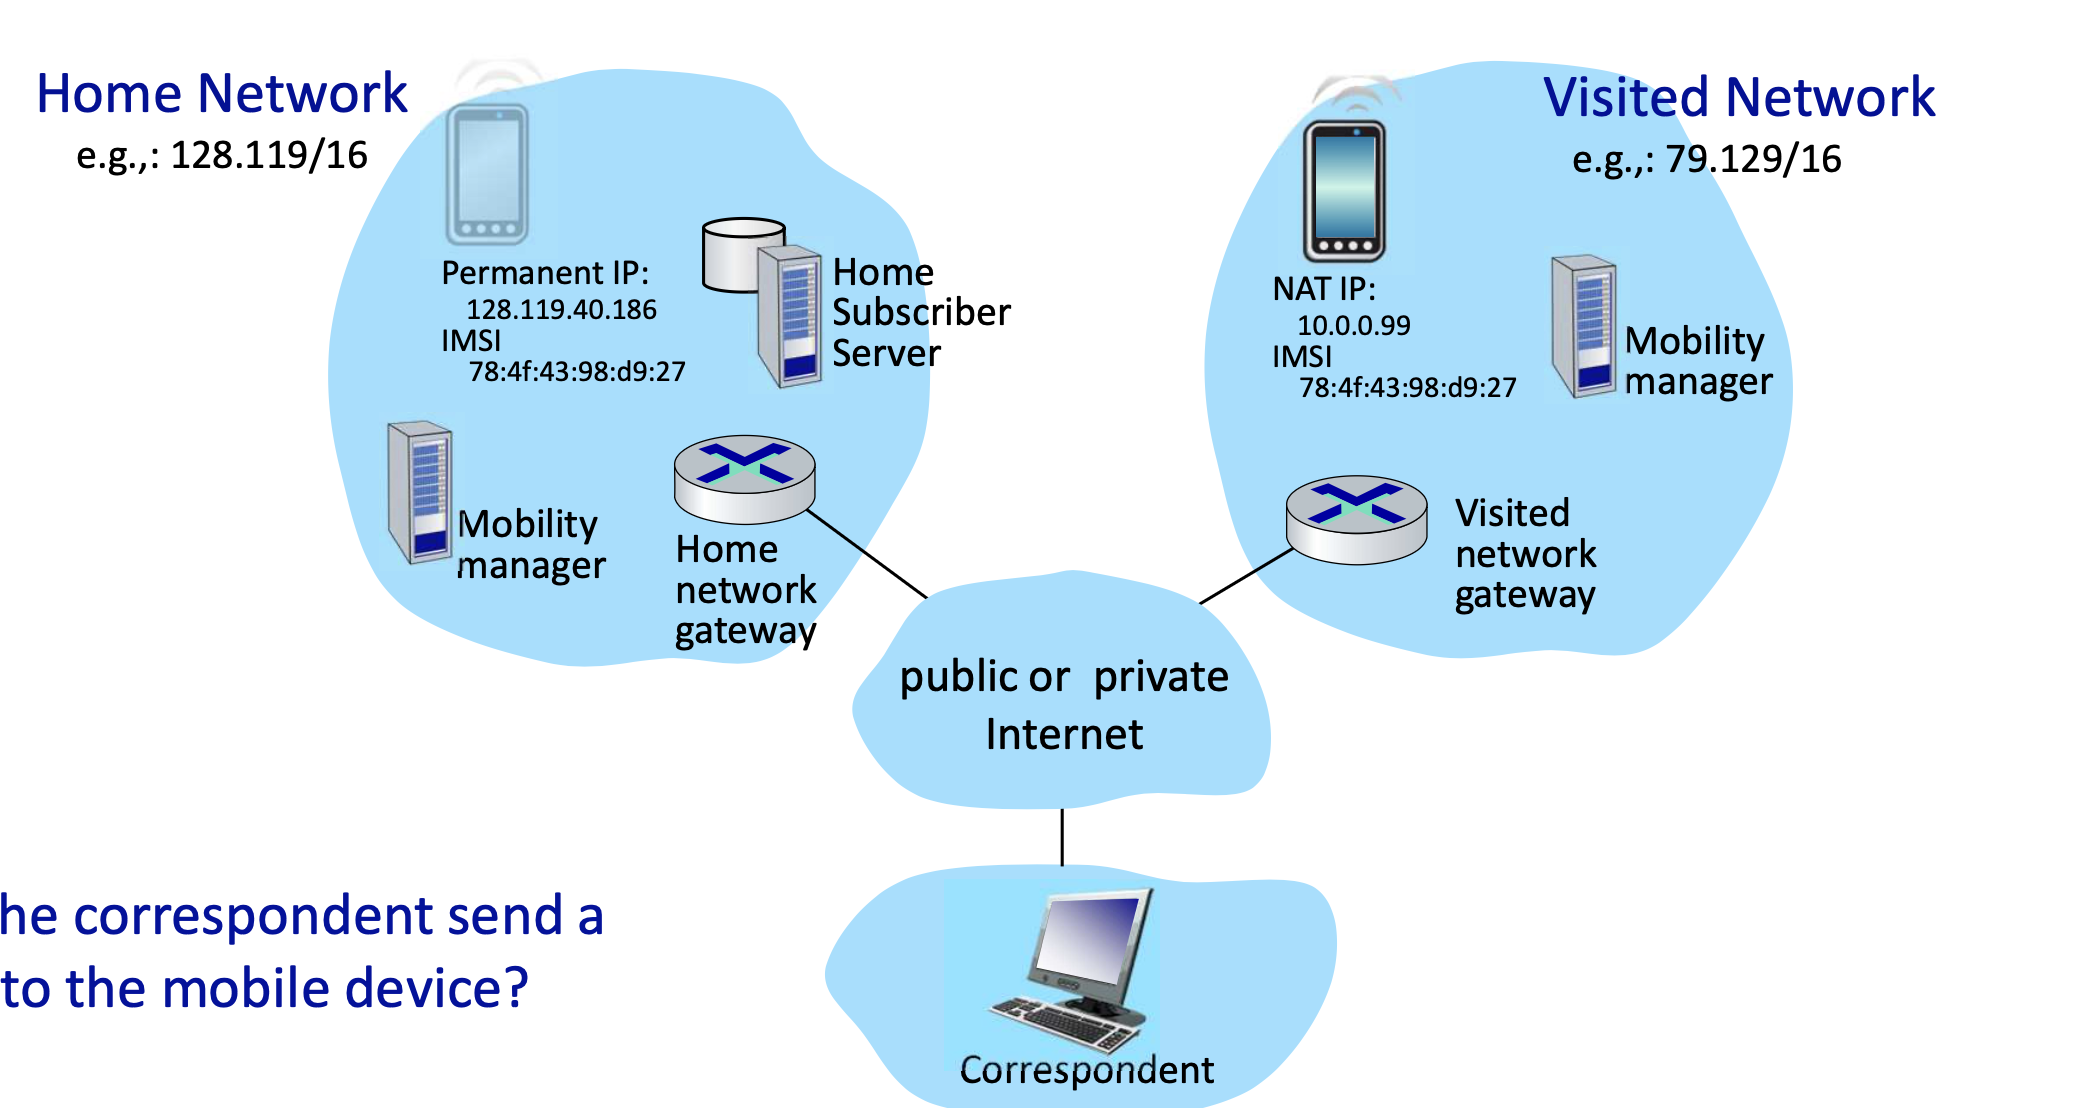
\includegraphics[keepaspectratio]{images/Pasted-image-20260313143711.png}}
\caption{Relazione tra home network e visited network in uno scenario di
roaming.}
\end{figure}

Le reti cellulari formano una ``rete di reti IP'' connesse via IPX (IP
eXchange). A differenza di Internet cablata o del Wi-Fi (dove
l'autenticazione è locale e la mobilità fluida è complessa), nelle reti
cellulari la mobilità è un servizio nativo di prima classe e l'identità
è legata alla SIM.

\subsection{Approcci alla Gestione della Mobilità: Registrazione e
Routing}\label{approcci-alla-gestione-della-mobilituxe0-registrazione-e-routing}

La home network deve sempre conoscere la posizione del dispositivo. Ciò
avviene tramite \textbf{registrazione}: il dispositivo si associa a un
\emph{mobility manager} nella rete visitata (es. MME), che comunica la
posizione all'HSS.

\begin{figure}
\centering
\pandocbounded{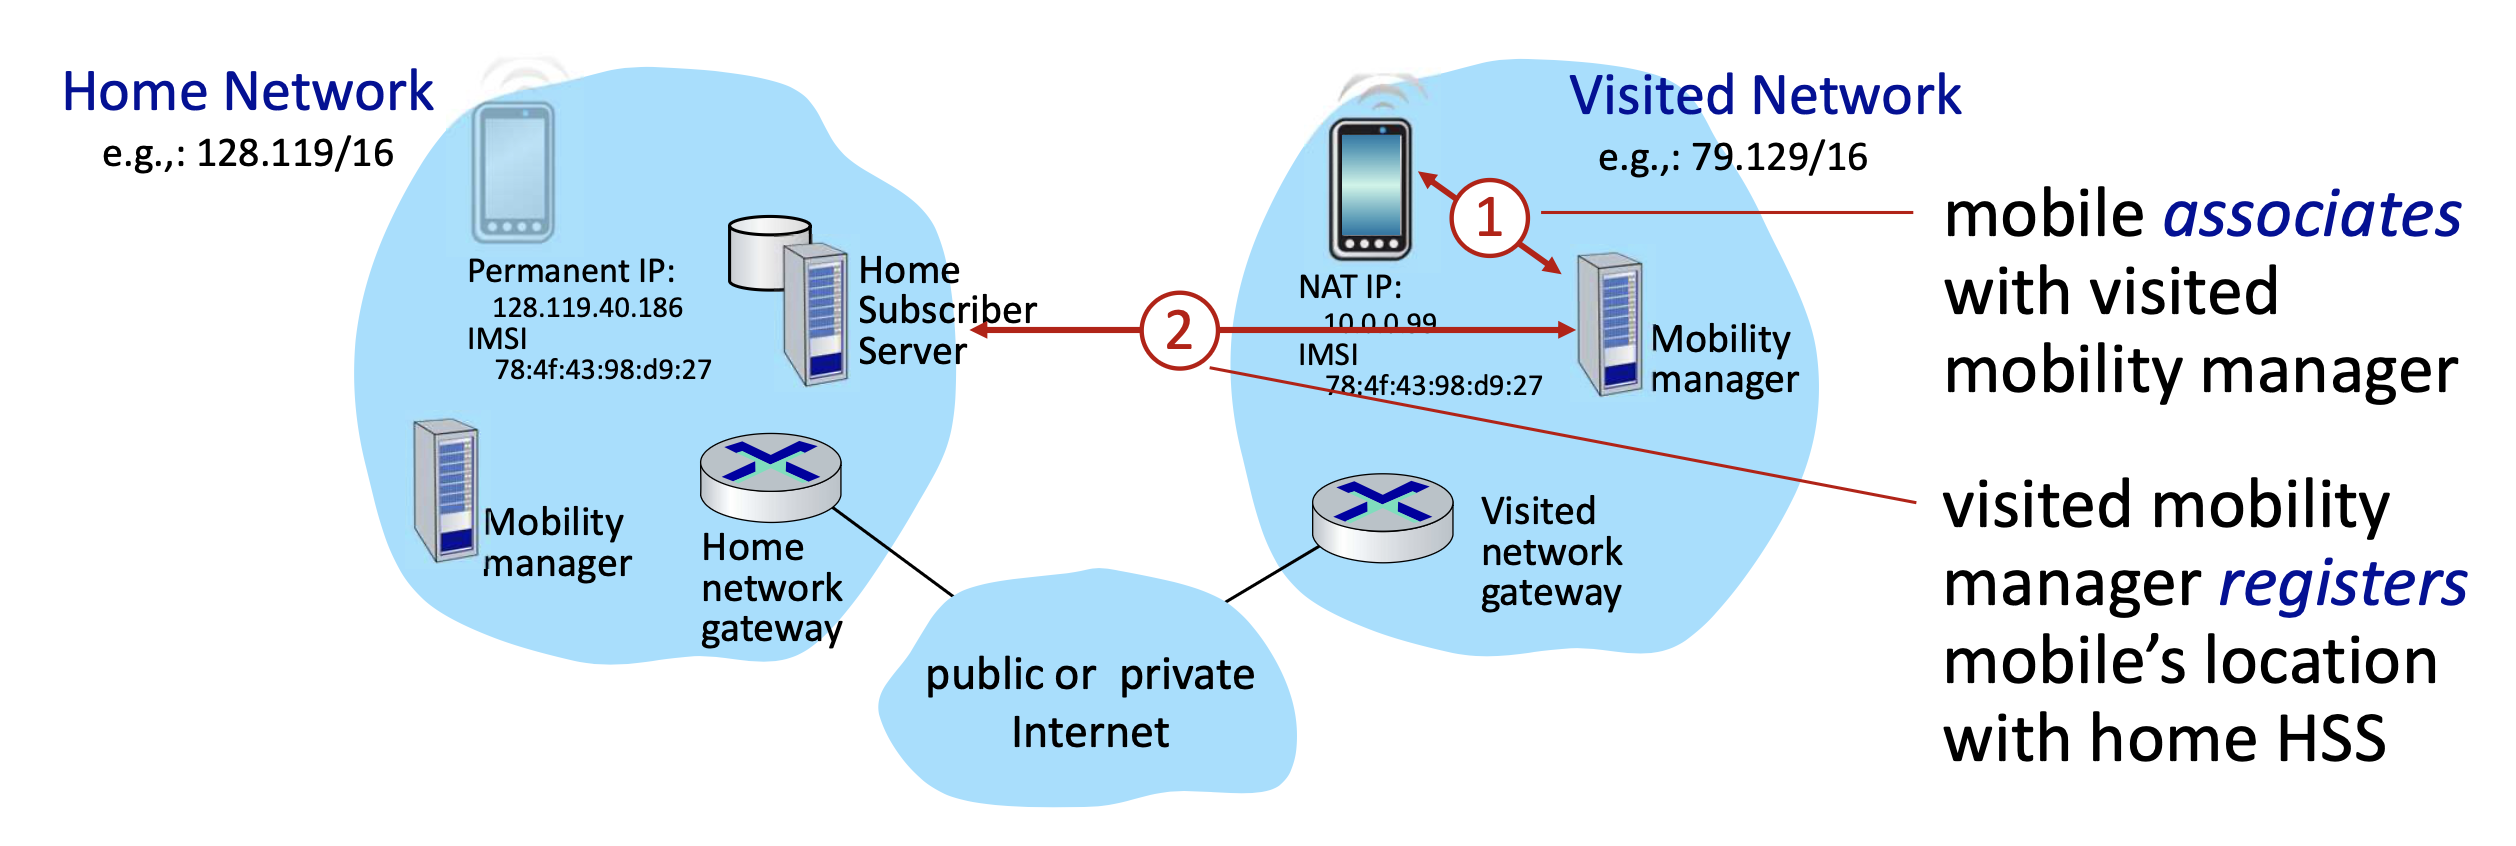
\includegraphics[keepaspectratio]{images/Pasted-image-20260313143813.png}}
\caption{Procedura di registrazione tra visited network e home network.}
\end{figure}

Per il recapito dei pacchetti, l'architettura sposta la complessità ai
margini della rete, con due possibili tecniche:

\begin{enumerate}
\def\labelenumi{\arabic{enumi}.}
\tightlist
\item
  \textbf{Routing Indiretto} (standard 4G LTE e Mobile IP): I pacchetti
  diretti al mobile sono inviati al gateway della home network, che li
  incapsula in un tunnel verso il gateway della rete visitata. Questo
  genera \emph{triangle routing} ma rende la mobilità trasparente al
  nodo corrispondente. Servono tre protocolli: associazione,
  registrazione e tunneling.
\item
  \textbf{Routing Diretto}: Il corrispondente interroga l'HSS per il
  care-of-address del dispositivo e manda i datagrammi direttamente.
  Elimina il triangle routing, ma gestire un cambio di rete a sessione
  in corso è molto complesso.
\end{enumerate}

\subsection{Il tunneling GTP: il pilastro della mobilità
4G/5G}\label{il-tunneling-gtp-il-pilastro-della-mobilituxe0-4g5g}

Il 4G adotta il \textbf{routing indiretto} tramite tunneling
\textbf{GTP-U}. Il datagramma originario emesso dall'UE viene
incapsulato con GTP e inviato dentro UDP all'S-GW, che lo re-incapsula
per il P-GW. Questo meccanismo mantiene gli \textbf{indirizzi IP
visibili a Internet fissi} (quelli di S-GW e P-GW). Durante un cambio di
cella, basta \textbf{aggiornare gli endpoint del tunnel GTP} (es.
l'indirizzo della Base Station). L'IP dell'UE resta inalterato e le
sessioni TCP non cadono.

\begin{figure}
\centering
\pandocbounded{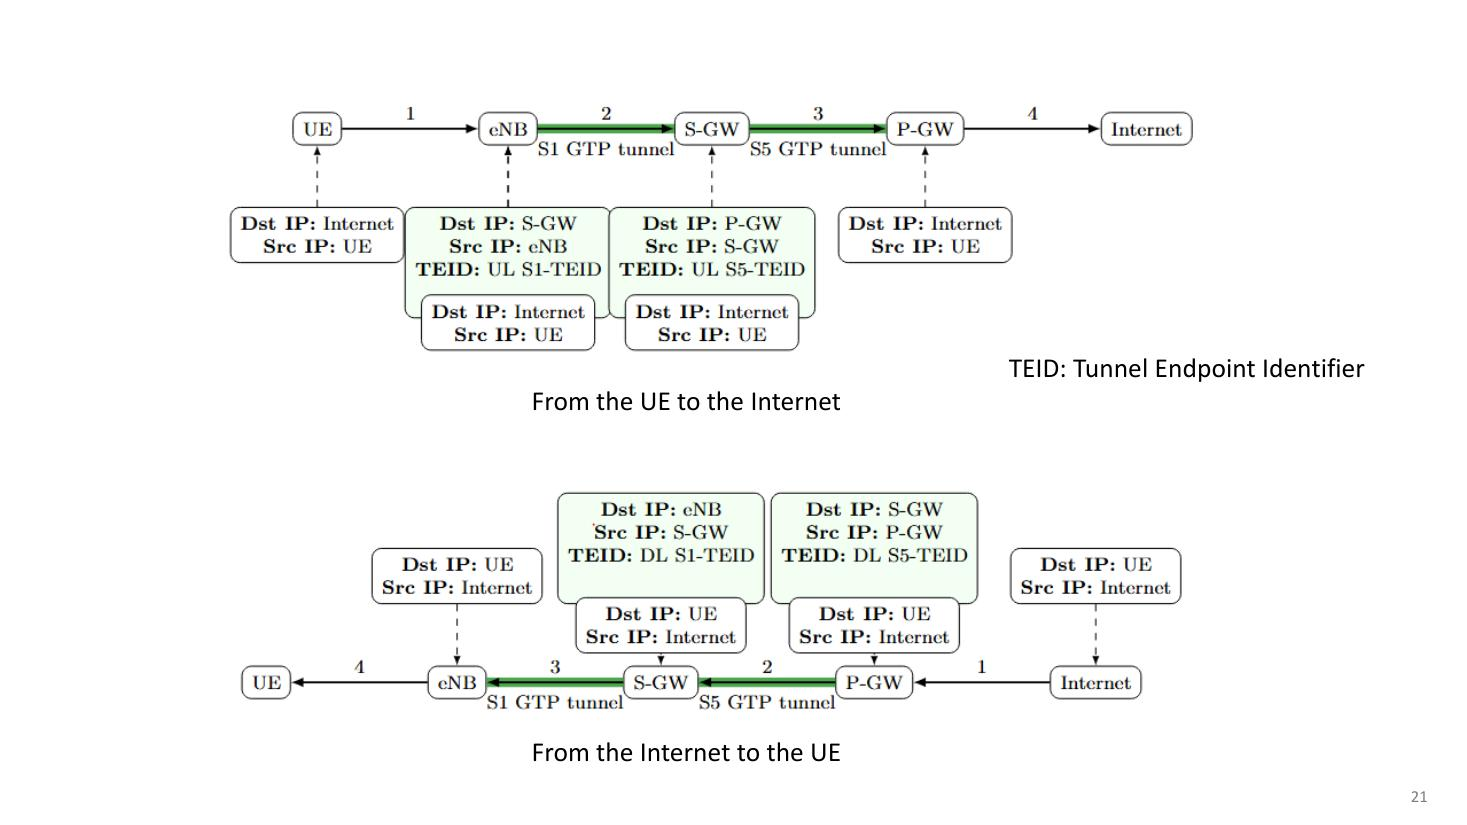
\includegraphics[keepaspectratio]{images/lezione-7-lab-mobile-networks-img-01.jpg}}
\caption{Composizione degli header GTP nel doppio senso del traffico per
preservare l'IP sorgente e destinazione.}
\end{figure}

\begin{center}\rule{0.5\linewidth}{0.5pt}\end{center}

\section{Mobilità Pratica: Handover, Sleep Modes e
Associazione}\label{mobilituxe0-pratica-handover-sleep-modes-e-associazione}

\subsection{Associazione e Sleep
Modes}\label{associazione-e-sleep-modes}

Per preservare la batteria, i dispositivi vanno in \textbf{sleep mode}
(light o deep). In deep sleep, al risveglio, potrebbero aver cambiato
cella e devono ristabilire l'associazione per ricevere messaggi di
\textbf{paging} (broadcastati dall'MME). L'associazione avviene leggendo
i segnali di sincronizzazione (primary e secondary) e i dati di sistema
broadcastati dalla BS ogni 5 ms.

\subsection{Handover tra Base Station}\label{handover-tra-base-station}

Quando la qualità del segnale degrada, il dispositivo si sposta su
un'altra BS senza interrompere le connessioni (handover).

\begin{enumerate}
\def\labelenumi{\arabic{enumi}.}
\tightlist
\item
  La \textbf{BS sorgente} decide l'handover e invia una \emph{Handover
  Request} alla \emph{target BS}.
\item
  La \textbf{target BS} pre-alloca risorse e risponde con \emph{ACK}.
\item
  La \textbf{BS sorgente} notifica l'UE, che inizia a trasmettere sulla
  nuova cella.
\item
  La \textbf{BS sorgente} fa forward dei datagrammi in arrivo verso la
  target BS per non perderli.
\item
  La \textbf{target BS} informa l'\textbf{MME}.
\item
  L'\textbf{MME} istruisce l'\textbf{S-GW} di aggiornare l'endpoint del
  tunnel GTP alla nuova target BS.
\item
  Il traffico fluisce sul \textbf{nuovo tunnel}.
\end{enumerate}

\begin{callouttip}{Decisione dell’handover}

La decisione dell'handover e la scelta della target BS spettano alla
\textbf{BS sorgente}, non all'MME, il quale interviene solo alla fine
per aggiornare il piano dati.

\end{callouttip}

\begin{figure}
\centering
\pandocbounded{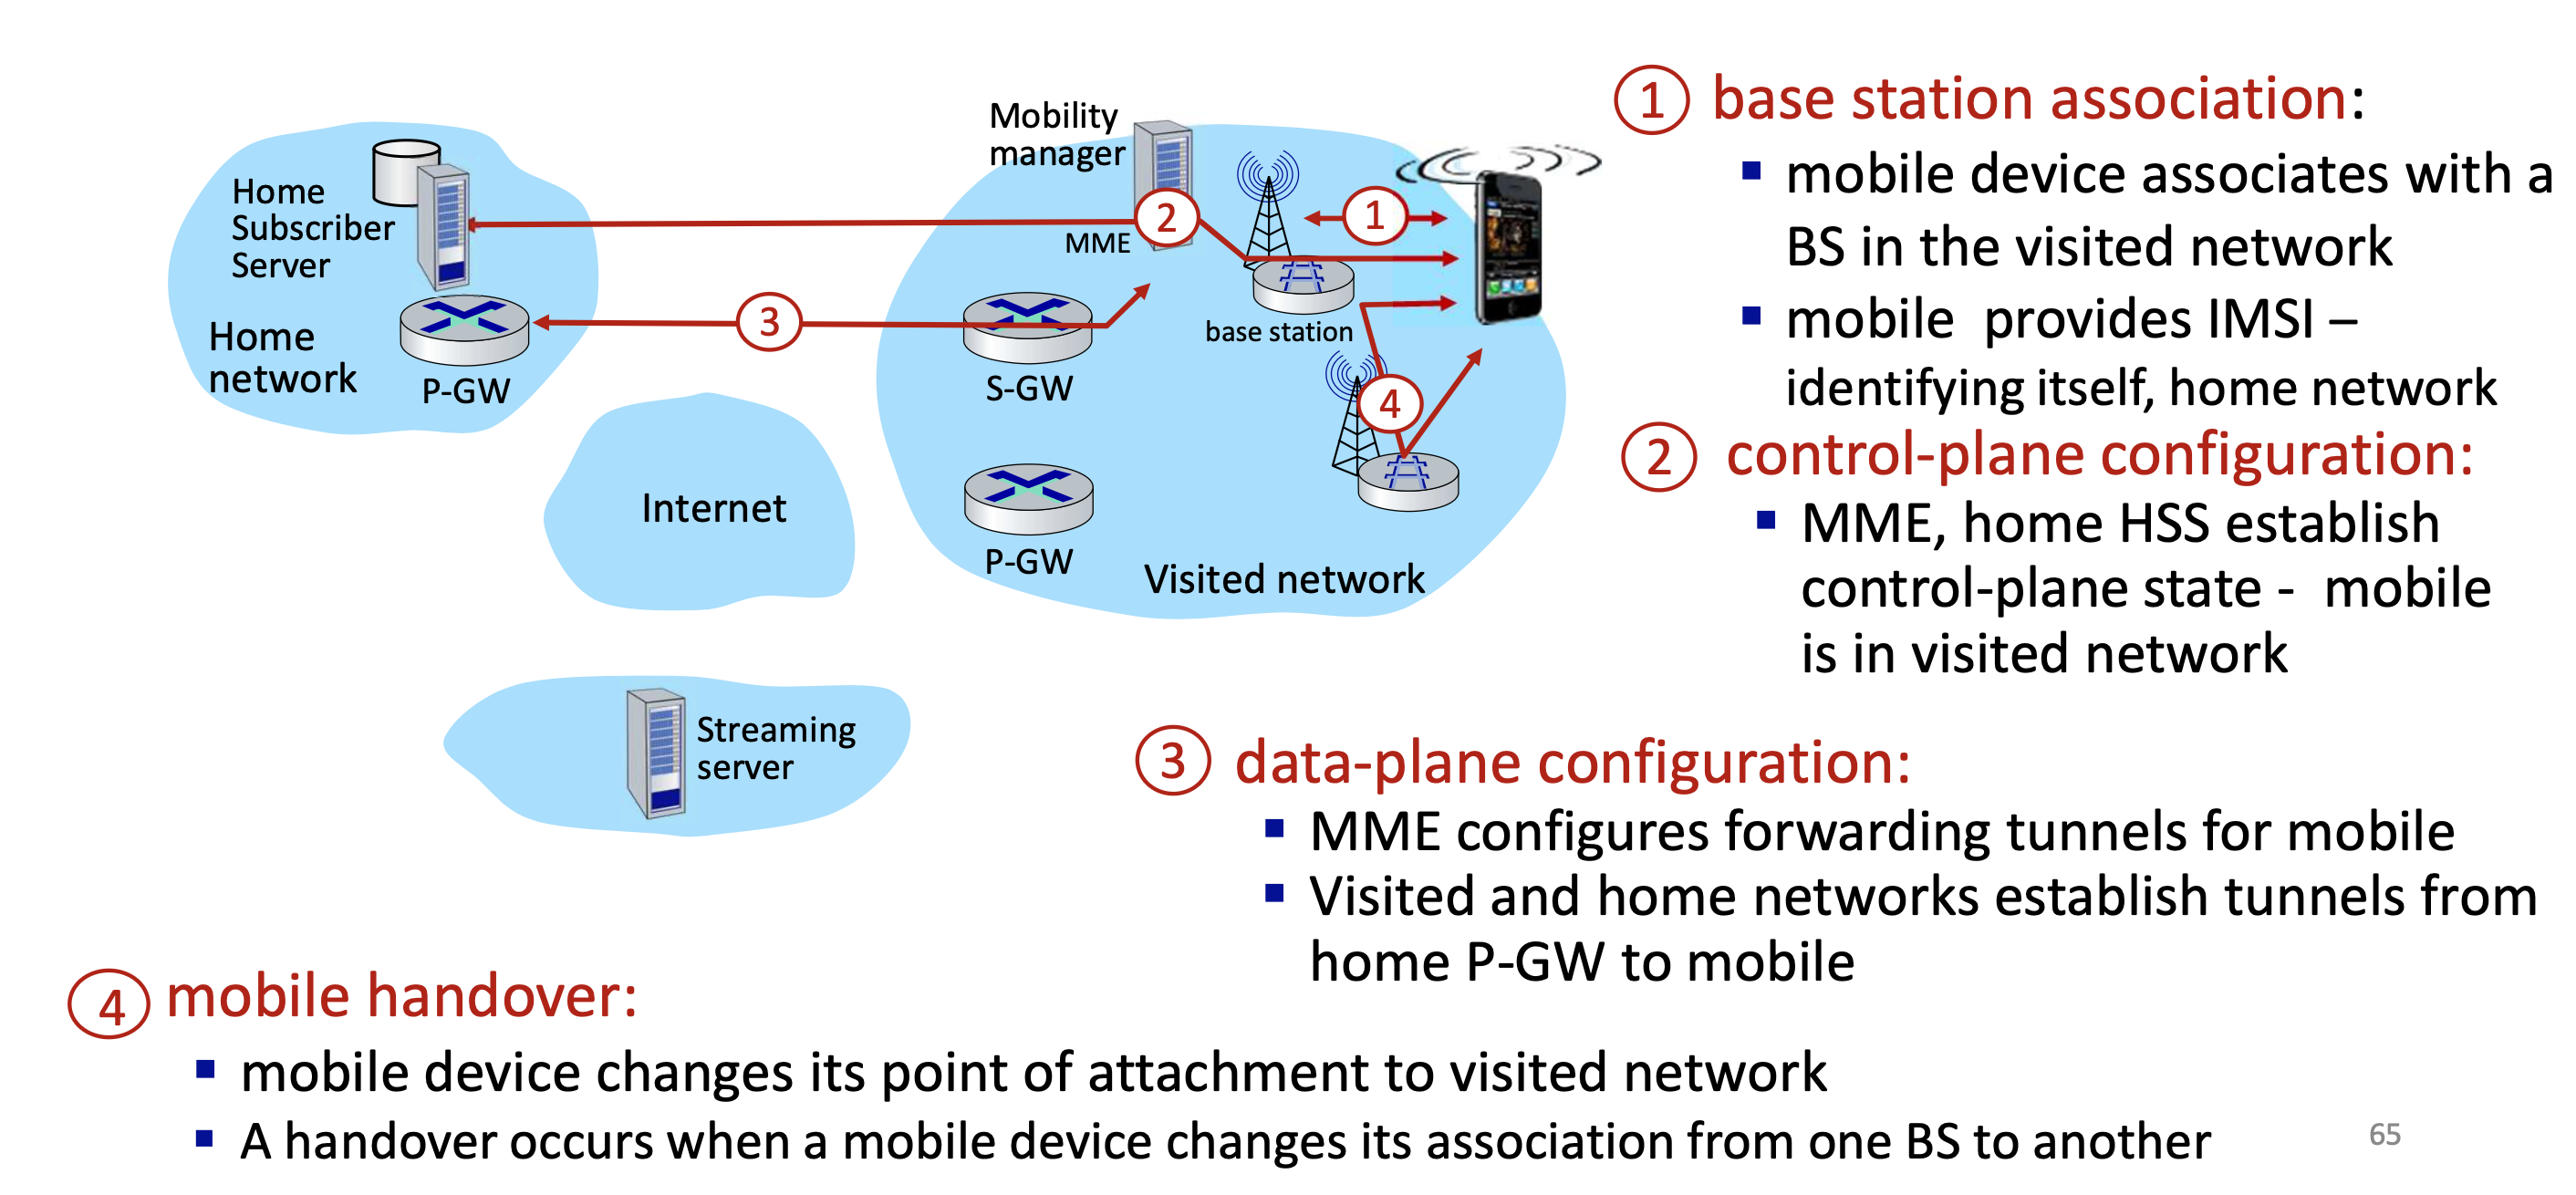
\includegraphics[keepaspectratio]{images/Pasted-image-20260313145859.png}}
\caption{Sequenza di messaggi durante un handover tra due Base Station
in 4G.}
\end{figure}

\begin{center}\rule{0.5\linewidth}{0.5pt}\end{center}

\section{Lo stack del Data Plane LTE}\label{lo-stack-del-data-plane-lte}

Sul primo hop (UE ↔ BS), si aggiungono quattro livelli sotto l'IP: 1.
\textbf{PDCP}: compressione header e crittografia. 2. \textbf{RLC}:
frammentazione e link affidabile (ACK/NACK). 3. \textbf{MAC}: scheduling
risorse radio, rilevazione errori. 4. \textbf{Physical Layer}:
modulazione OFDM, distribuisce time slot da 0.5 ms su sottoportanti
ortogonali, raggiungendo centinaia di Mbps.

\begin{figure}
\centering
\pandocbounded{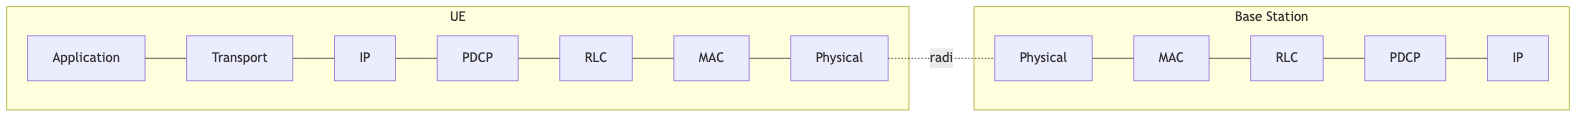
\includegraphics[keepaspectratio,alt={Stack protocollare del data plane LTE sull'interfaccia radio. Mostra come i livelli PDCP, RLC, MAC e Physical si frappongono tra IP e la trasmissione radio fisica.}]{images/mermaid-03-reti-mobili-tradizionali-04.png}}
\caption{Stack protocollare del data plane LTE sull'interfaccia radio.
Mostra come i livelli PDCP, RLC, MAC e Physical si frappongono tra IP e
la trasmissione radio fisica.}
\end{figure}

\begin{center}\rule{0.5\linewidth}{0.5pt}\end{center}

\section{Sicurezza e autenticazione in 4G LTE: il protocollo
AKA}\label{sicurezza-e-autenticazione-in-4g-lte-il-protocollo-aka}

Quando un UE arriva in una rete, deve \textbf{associarsi alla BS} e
\textbf{autenticarsi mutamente} con la rete. La SIM fornisce l'identità
globale e la chiave segreta \(K_{HSS\text{-}M}\). L'HSS fa da ``ultimate
authenticator'', ma in 4G la decisione passa per l'MME visitato.

Il protocollo \textbf{AKA} (Authentication and Key Agreement) è basato
su challenge-response simmetrica.

\begin{figure}
\centering
\pandocbounded{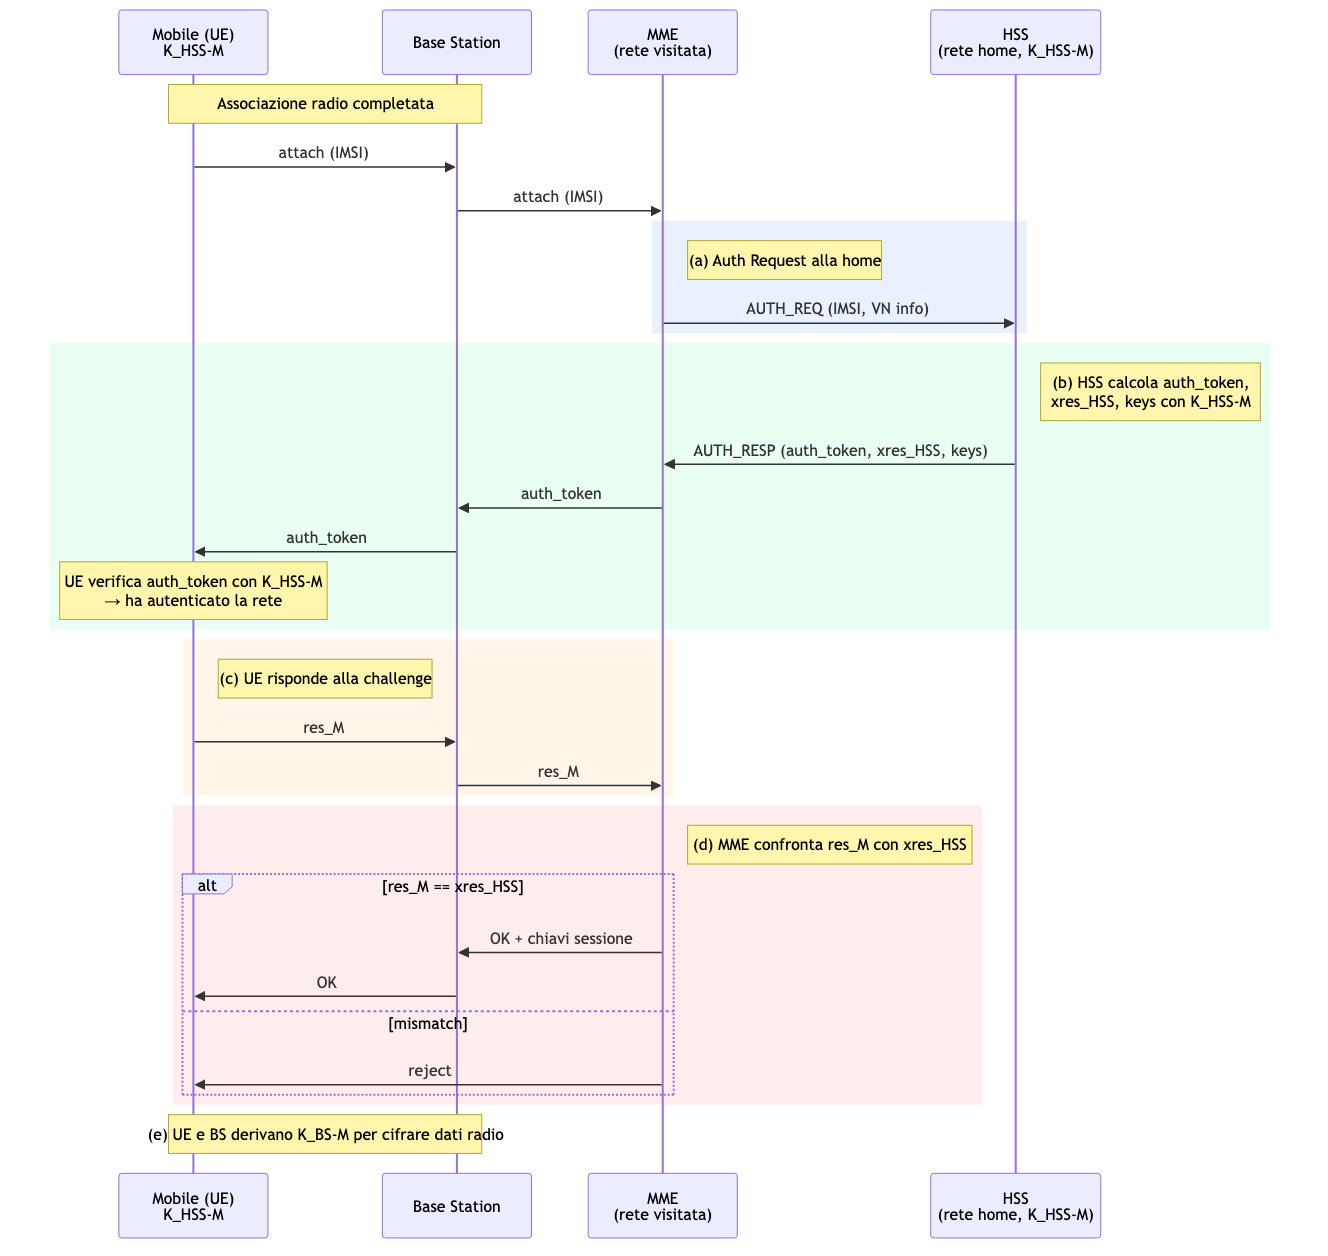
\includegraphics[keepaspectratio,alt={Sequence diagram del protocollo AKA in 4G LTE. Mostra l'autenticazione mutua challenge-response tra UE, MME visitato e HSS domestico tramite calcolo crittografico basato sulla chiave simmetrica della SIM.}]{images/mermaid-03-reti-mobili-tradizionali-05.png}}
\caption{Sequence diagram del protocollo AKA in 4G LTE. Mostra
l'autenticazione mutua challenge-response tra UE, MME visitato e HSS
domestico tramite calcolo crittografico basato sulla chiave simmetrica
della SIM.}
\end{figure}

\begin{enumerate}
\def\labelenumi{\arabic{enumi}.}
\tightlist
\item
  \textbf{Attach}: L'UE invia l'IMSI all'MME, che lo gira all'HSS.
\item
  \textbf{Challenge}: L'HSS usa la chiave segreta \(K_{HSS\text{-}M}\)
  per generare un \texttt{auth\_token}, la risposta attesa
  \texttt{xres\_HSS} e chiavi di sessione. Manda all'MME, che inoltra
  l'\texttt{auth\_token} all'UE. L'UE lo decifra e lo verifica.
  \textbf{L'UE ha autenticato la rete.}
\item
  \textbf{Risposta UE}: L'UE calcola \texttt{res\_M} con la sua
  \(K_{HSS\text{-}M}\) e lo invia all'MME.
\item
  \textbf{Verifica}: L'MME confronta \texttt{res\_M} con
  \texttt{xres\_HSS}. Se coincidono, \textbf{la rete ha autenticato
  l'UE}.
\item
  \textbf{Derivazione chiavi}: UE e BS derivano una chiave di sessione
  (es. AES) per cifrare il canale radio.
\end{enumerate}

\begin{calloutquestion}{Perché \\text\{res\}\_M = \\text\{xres\}\_\{HSS\} dimostra l’identità?}

Perché la funzione dipende dalla chiave segreta nota solo alla SIM e
all'HSS. Se i valori coincidono, l'UE possiede certamente la chiave.

\end{calloutquestion}

\begin{center}\rule{0.5\linewidth}{0.5pt}\end{center}

\section{La rivoluzione del 5G: prestazioni, architettura e
sicurezza}\label{la-rivoluzione-del-5g-prestazioni-architettura-e-sicurezza}

Il 5G (New Radio) alza le prestazioni con bande \textbf{FR1} (sub-6 GHz)
e \textbf{FR2} (mmWave fino a 52 GHz, richiede picocelle e antenne
MIMO), gestendo tre scenari: - \textbf{eMBB} (Enhanced Mobile
Broadband): larghezza di banda estrema per video 4K, VR. -
\textbf{URLLC} (Ultra Reliable Low-Latency): latenza \textless1ms per
guida autonoma, industria 4.0. - \textbf{mMTC} (Massive Machine Type
Comms): connessioni IoT massicce, ultra-low power, 1M nodi/km².

\subsection{5G Core e Service Based Architecture
(SBA)}\label{g-core-e-service-based-architecture-sba}

La \textbf{NG-Core} del 5G è cloud-native. Basata su \textbf{Network
Function Virtualization (NFV)}, le funzioni di rete sono microservizi
(container/VM) che si parlano tramite \textbf{Service-Based Interface
(SBI)} (REST HTTP/2).

{\def\LTcaptype{none} % do not increment counter
\begin{longtable}[]{@{}
  >{\raggedright\arraybackslash}p{(\linewidth - 4\tabcolsep) * \real{0.3333}}
  >{\raggedright\arraybackslash}p{(\linewidth - 4\tabcolsep) * \real{0.3333}}
  >{\raggedright\arraybackslash}p{(\linewidth - 4\tabcolsep) * \real{0.3333}}@{}}
\toprule\noalign{}
\begin{minipage}[b]{\linewidth}\raggedright
\textbf{Componente 4G}
\end{minipage} & \begin{minipage}[b]{\linewidth}\raggedright
\textbf{Corrispettivo 5G}
\end{minipage} & \begin{minipage}[b]{\linewidth}\raggedright
\textbf{Funzione}
\end{minipage} \\
\midrule\noalign{}
\endhead
\bottomrule\noalign{}
\endlastfoot
\textbf{eNB} & \textbf{gNB} & Radio 5G modulare, divisa in Distributed e
Central Unit. \\
\textbf{S-GW + P-GW} & \textbf{UPF} (User Plane Function) & Inoltra
traffico RAN-Internet. Distribuibile all'edge. \\
\textbf{MME} & \textbf{AMF + SMF} & \textbf{AMF}: mobilità,
autenticazione. \textbf{SMF}: gestione sessioni. \\
\textbf{HSS} & \textbf{AUSF + UDM} & \textbf{AUSF}: autenticazione.
\textbf{UDM}: dati abbonamento/identità. \\
\textbf{PCRF} & \textbf{PCF} & Policy Control Function. \\
\end{longtable}
}

Funzioni di supporto cloud-native (statelessness): \textbf{SDSF/UDSF}
per archiviazione, \textbf{NRF} per service discovery, \textbf{NEF} per
API verso terzi, e \textbf{NSSF} per il \textbf{Network Slicing}.

La distribuzione dell'\textbf{UPF} all'edge abilita il
\textbf{Multi-Access Edge Computing (MEC)}, fondamentale per abbattere
le latenze (URLLC).

\begin{figure}
\centering
\pandocbounded{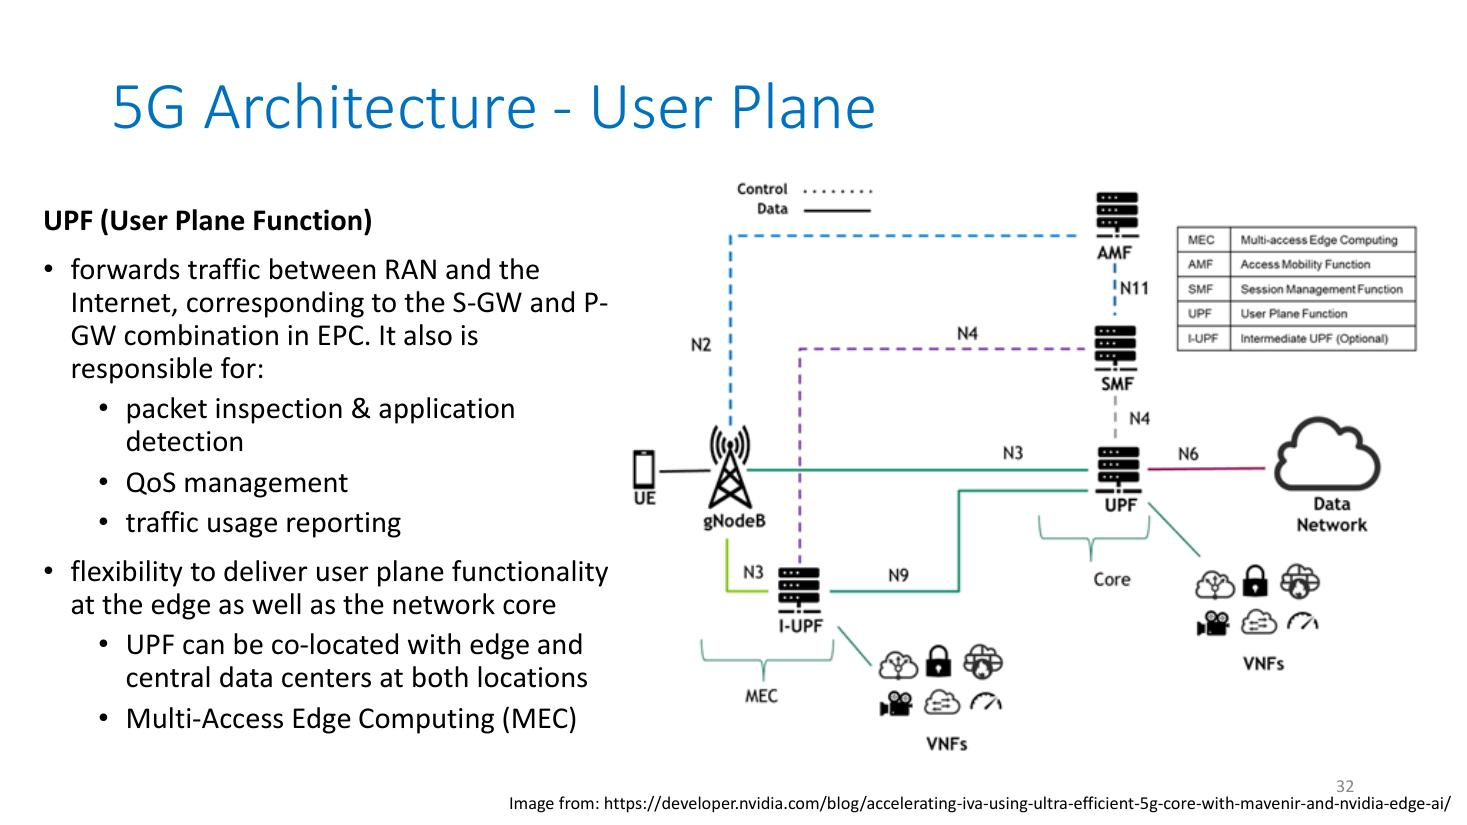
\includegraphics[keepaspectratio]{images/lezione-7-lab-mobile-networks-img-02.jpg}}
\caption{Architettura 5G User Plane: l'UPF distribuito e il MEC all'edge
abilitano elaborazione a bassissima latenza.}
\end{figure}

\subsection{Opzioni di deployment}\label{opzioni-di-deployment}

L'adozione varia fra \textbf{Non-Standalone (NSA)} (radio 5G per i dati,
piano di controllo appoggiato sull'EPC 4G) e \textbf{Standalone (SA)}
(rete 5G pura con NG-Core). In Europa domina ancora NSA.

\subsection{Sicurezza in 5G vs 4G}\label{sicurezza-in-5g-vs-4g}

Il 5G risolve due falle storiche: 1. \textbf{Decisione di
autenticazione}: In 5G la decisione finale è presa dalla \textbf{rete
home} (AUSF), mentre l'AMF visitato è solo un tramite, riducendo
l'impatto se una rete visitata viene compromessa. 2.
\textbf{Trasmissione dell'IMSI}: In 4G l'IMSI viaggia in chiaro alla
connessione (esponendo ad attacchi \emph{IMSI catcher}). Il 5G cifra
l'IMSI con la \textbf{chiave pubblica della home network} (creando il
SUCI), schermando l'identità.

\begin{center}\rule{0.5\linewidth}{0.5pt}\end{center}

\section{Mobile IP e Impatto sui Protocolli di
Trasporto}\label{mobile-ip-e-impatto-sui-protocolli-di-trasporto}

L'architettura \textbf{Mobile IP} (RFC 5944) fu uno standard teorico
precedente che univa concetti simili al routing indiretto (con
\emph{home agent} e \emph{foreign agent}), ma non ha avuto successo
commerciale a differenza delle reti 4G. Sui protocolli di trasporto
(TCP), il canale radio mobile crea problemi. Perdite per interferenze o
interruzioni transitorie in handover inducono TCP, nativo su fili, a
ridurre drasticamente la \emph{congestion window} interpretando gli
errori radio come congestioni di rete, portando a cali inopportuni di
throughput.

\begin{center}\rule{0.5\linewidth}{0.5pt}\end{center}

\begin{calloutnote}{Sintesi}

Dalle reti analogiche si è passati all'All-IP Core del 4G (con
separazione control/data plane) e alla Service Based Architecture 5G
basata su microservizi e network slicing. La mobilità è gestita tramite
tunneling GTP (routing indiretto), mantenendo le sessioni IP attive
durante il passaggio tra celle. L'autenticazione è garantita dal
protocollo challenge-response AKA basato su SIM, reso più sicuro in 5G
grazie alla crittografia a chiave pubblica per l'identità (IMSI) e
all'accentramento delle decisioni di trust nella Home Network. Il 5G
apre nuovi scenari a banda altissima e latenza ridotta (MEC) ma eredita,
nei livelli superiori, i problemi di efficienza TCP su mezzi con errori
frequenti.

\end{calloutnote}

\begin{calloutquestion}{Possibili domande d’esame}

- Differenze tra routing indiretto e diretto, e concetto di triangle
routing. - Tre protocolli necessari per implementare routing indiretto
in 4G. - I ruoli di MME, HSS, S-GW, P-GW, e la loro mappatura in 5G
(AMF, SMF, UPF, ecc.). - Come il tunneling GTP supporta la mobilità
mantenendo le sessioni TCP attive. - La procedura di handover tra due
Base Station e chi la decide. - Il protocollo AKA: descrizione, calcolo
crittografico e mutua autenticazione. - Le due differenze di sicurezza
cruciali tra 4G e 5G (IMSI catcher e trust model). - Cos'è la Service
Based Architecture e perché il 5G usa NRF/UDSF. - I tre scenari
applicativi del 5G (eMBB, URLLC, mMTC) e il ruolo dell'UPF/MEC. - Perché
le perdite radio degradano le prestazioni TCP?

\end{calloutquestion}

\newpage

\chapter{04 - Reti Mobili Software Virtualizzate e
Slicing}\label{reti-mobili-software-virtualizzate-e-slicing}

\section{Reti Mobili Software Virtualizzate e
Slicing}\label{reti-mobili-software-virtualizzate-e-slicing-1}

\subsection{1. Software Defined Networking (SDN) ed
Architettura}\label{software-defined-networking-sdn-ed-architettura}

\subsubsection{Introduzione}\label{introduzione}

Il \textbf{Software Defined Networking} è un paradigma architetturale
che separa nettamente il \textbf{piano di controllo} (\emph{control
plane}) dal \textbf{piano dati} (\emph{data plane}). Questa astrazione
abilita configurazioni e operazioni dinamiche a livello programmatico,
eliminando la rigidità dei dispositivi tradizionali.

\subsection{Motivazioni ed Evoluzione del
Traffico}\label{motivazioni-ed-evoluzione-del-traffico}

Le reti tradizionali faticano a gestire la complessità e la variabilità
del traffico moderno (cloud, big data, IoT). La domanda è caratterizzata
da dinamiche \emph{time-variant}, \emph{spatially dynamic} e
\emph{application-sensitive}. - \textbf{Dominio del traffico East-West}:
Oltre il 70\% del traffico nei data center è interno tra server, mentre
le architetture classiche a tre livelli erano ottimizzate per traffico
North-South (client-server). - \textbf{Limiti strutturali}: Le reti
convenzionali soffrono di un'architettura statica e frammentata,
incoerenza delle policy (enforced localmente) e vendor lock-in a causa
di hardware proprietario con interfacce chiuse.

\begin{figure}
\centering
\pandocbounded{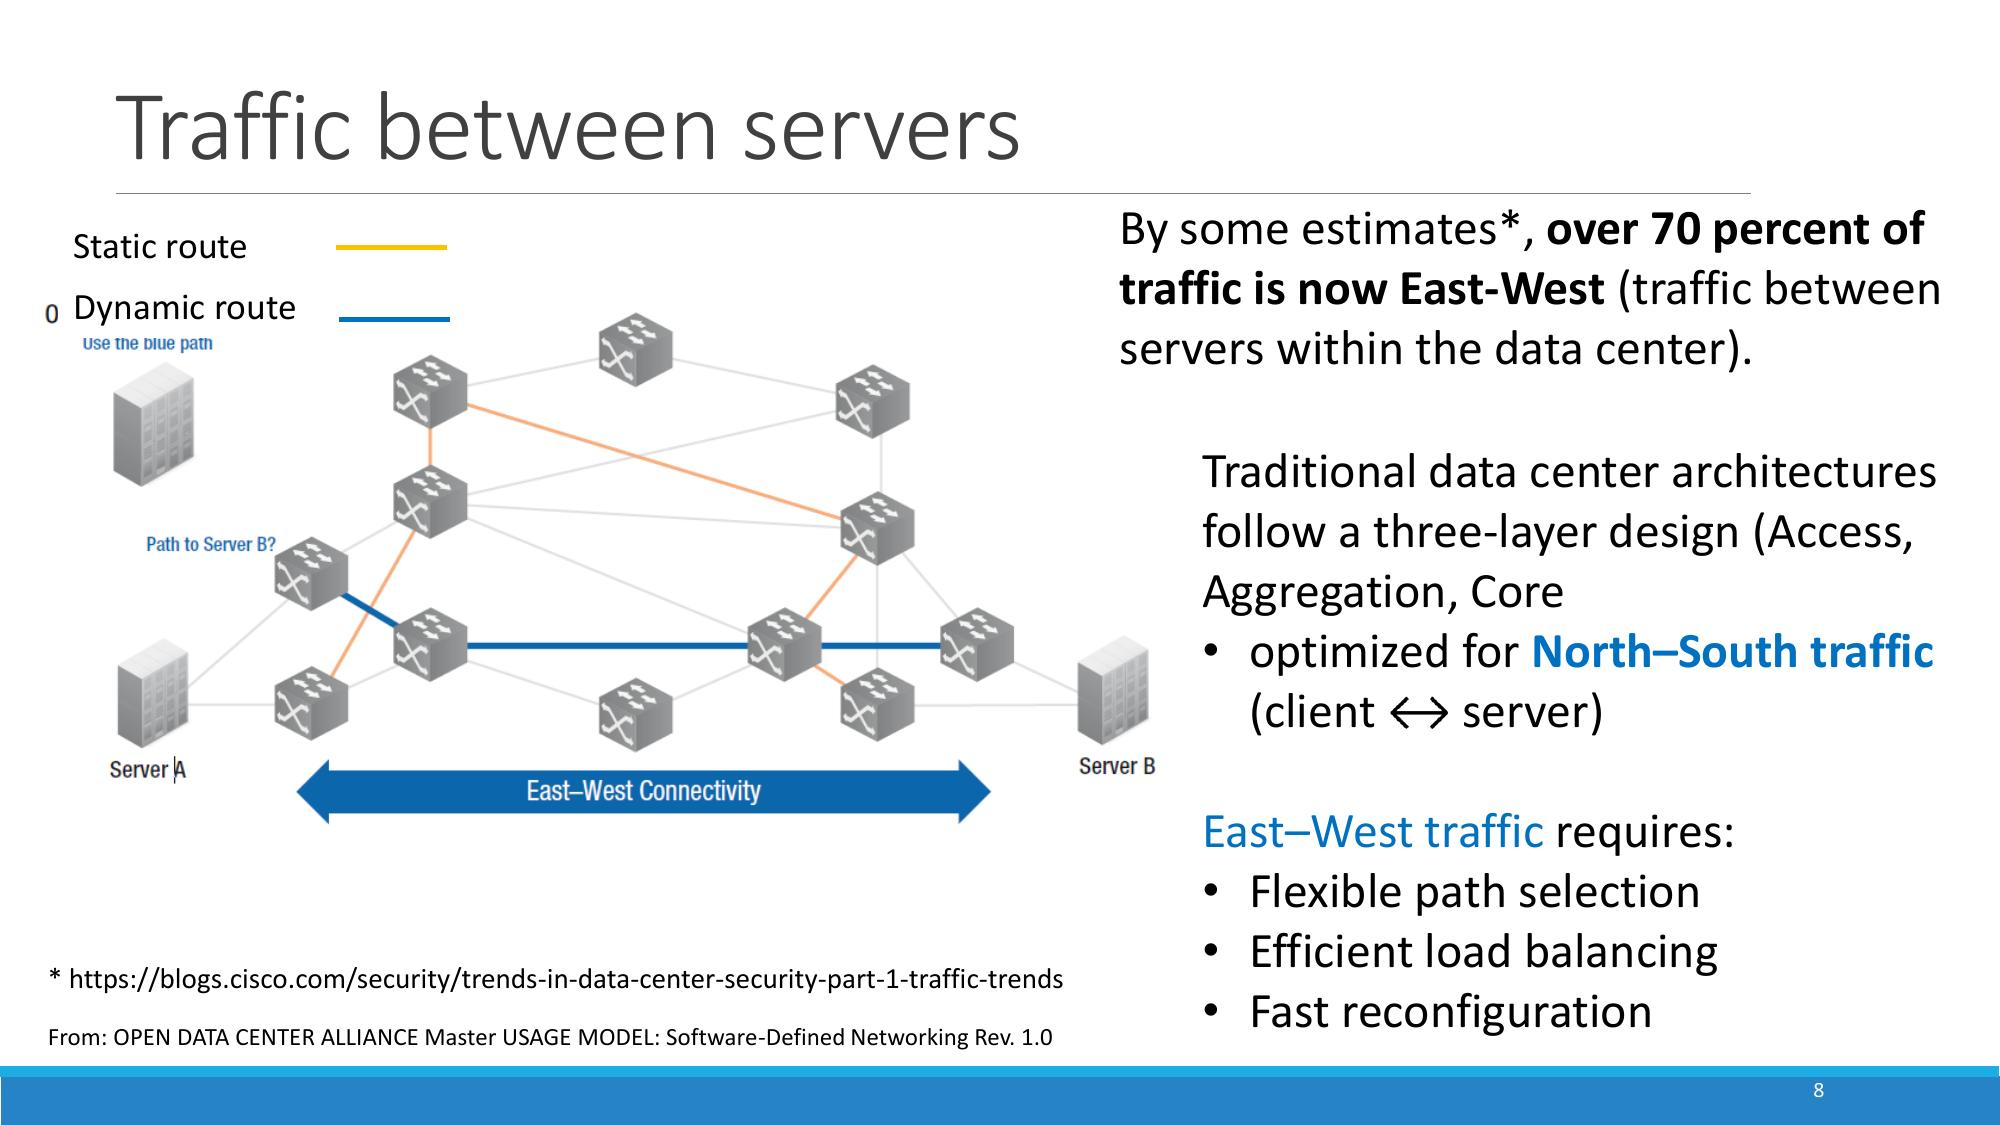
\includegraphics[keepaspectratio]{images/lezione-15-lab-sdn-architecture-img-01.jpg}}
\caption{1 --- Traffico East-West nei data center.}
\end{figure}

\subsection{La Separazione tra Data Plane e Control
Plane}\label{la-separazione-tra-data-plane-e-control-plane}

\begin{itemize}
\tightlist
\item
  \textbf{Data Plane (Forwarding)}: smistamento istantaneo dei pacchetti
  su scala temporale breve (\emph{fast timescales}).
\item
  \textbf{Control Plane (Routing)}: determinazione dei percorsi da
  sorgente a destinazione su scala temporale più lunga (\emph{slow
  timescales}).
\end{itemize}

Nel routing tradizionale, l'unico ``knob'' per il traffic engineering
sono i pesi dei link: non è possibile forzare percorsi specifici senza
alterare globalmente il routing, fare load balancing su più percorsi
uguali, o differenziare per flusso a parità di destinazione.

\begin{figure}
\centering
\pandocbounded{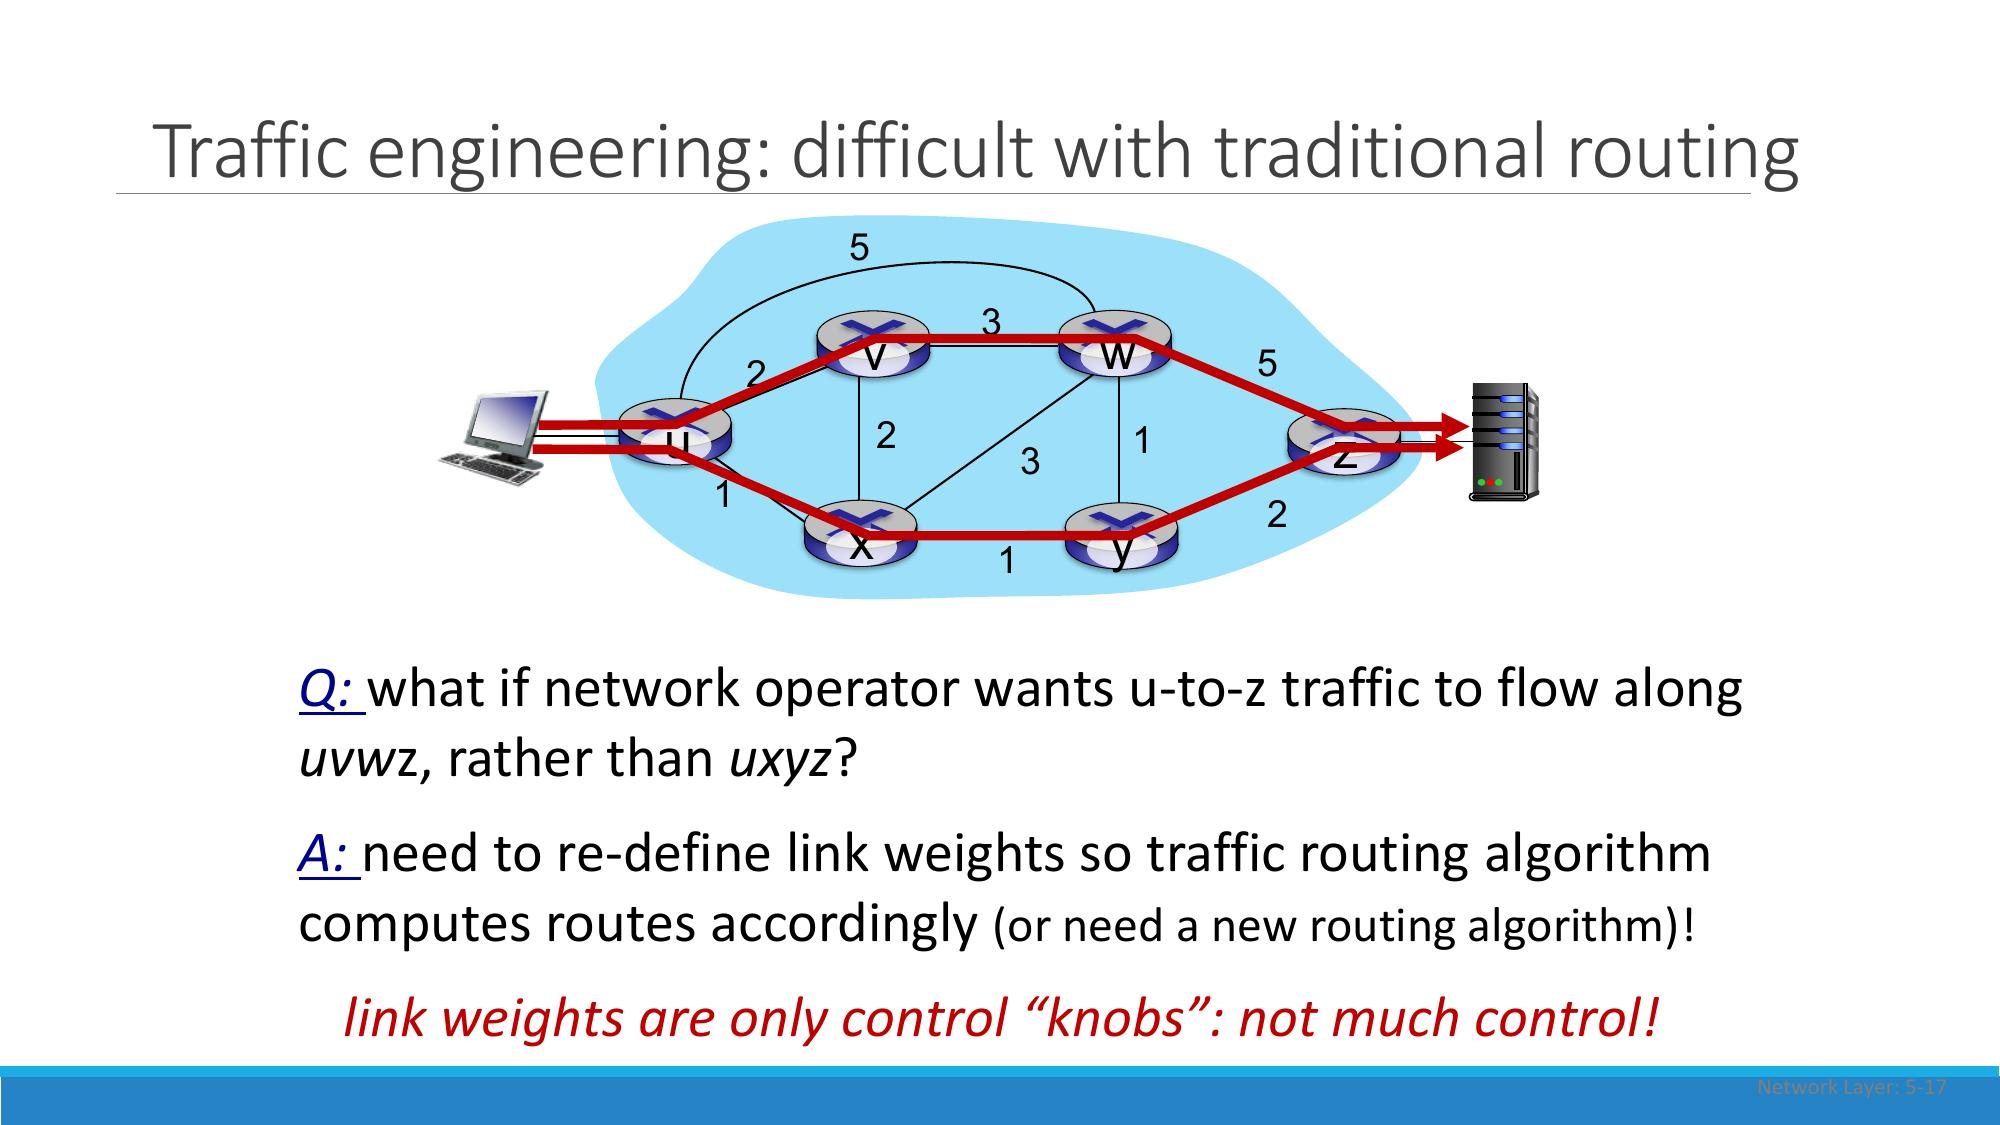
\includegraphics[keepaspectratio]{images/lezione-15-lab-sdn-architecture-img-02.jpg}}
\caption{2 --- Limiti del routing tradizionale.}
\end{figure}

\subsection{Il Paradigma SDN: Centralizzazione
Logica}\label{il-paradigma-sdn-centralizzazione-logica}

SDN sposta la logica di controllo in un controller remoto centralizzato
logicamente, calcolando le forwarding table globalmente in modo
consistente:
\[ \mathcal{F}: S(t) \rightarrow \{T_1, T_2, \ldots, T_n\} \] dove
\(S(t)\) include topologia, stato e policy.

\begin{figure}
\centering
\pandocbounded{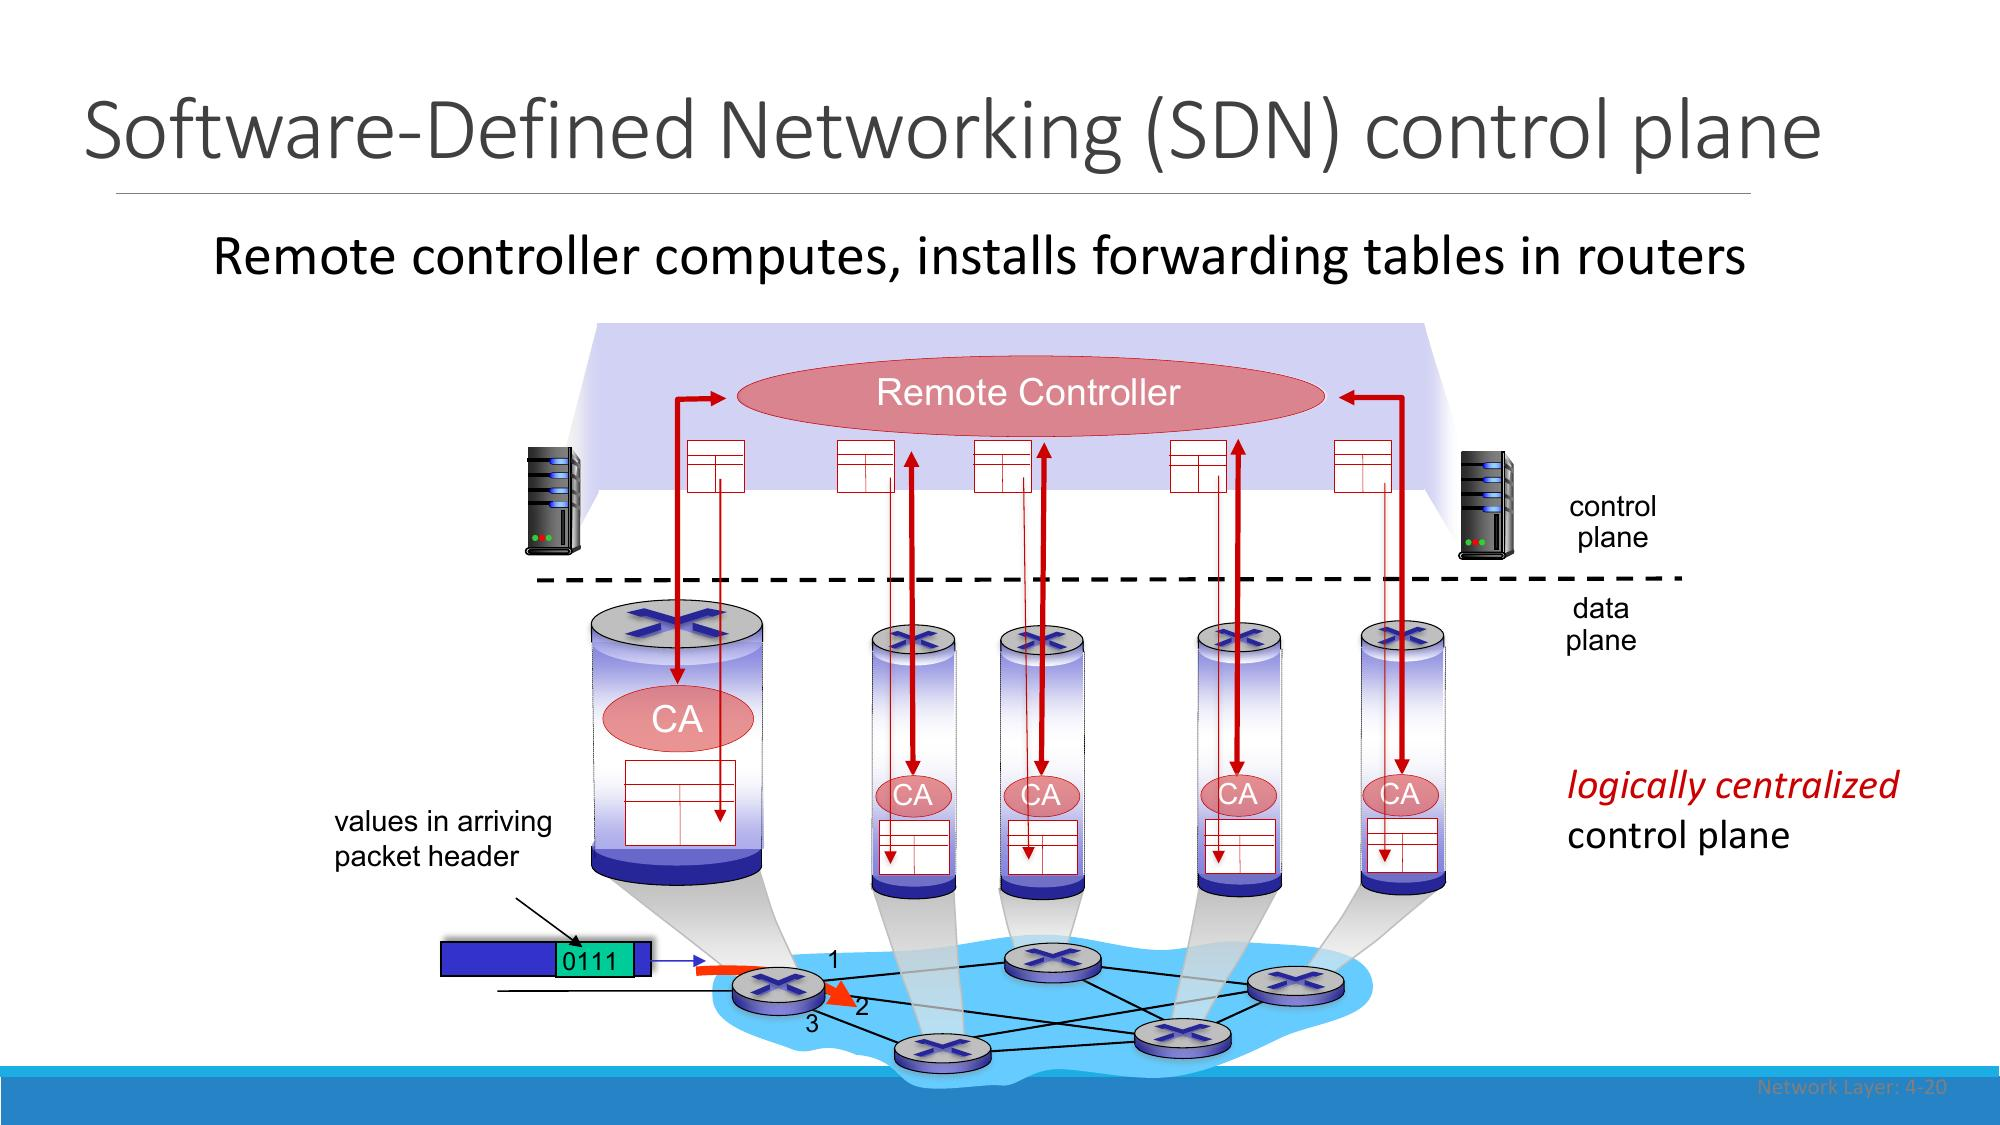
\includegraphics[keepaspectratio]{images/lezione-15-lab-sdn-architecture-img-03.jpg}}
\caption{3 --- Modello SDN con Remote Controller.}
\end{figure}

I quattro pilastri: 1. \textbf{Generalized flow-based forwarding}. 2.
\textbf{Separazione control plane / data plane}. 3. \textbf{Control
plane esterno agli switch}. 4. \textbf{Programmabilità} tramite
applicazioni.

\subsection{Architettura SDN a Tre
Livelli}\label{architettura-sdn-a-tre-livelli}

\begin{figure}
\centering
\pandocbounded{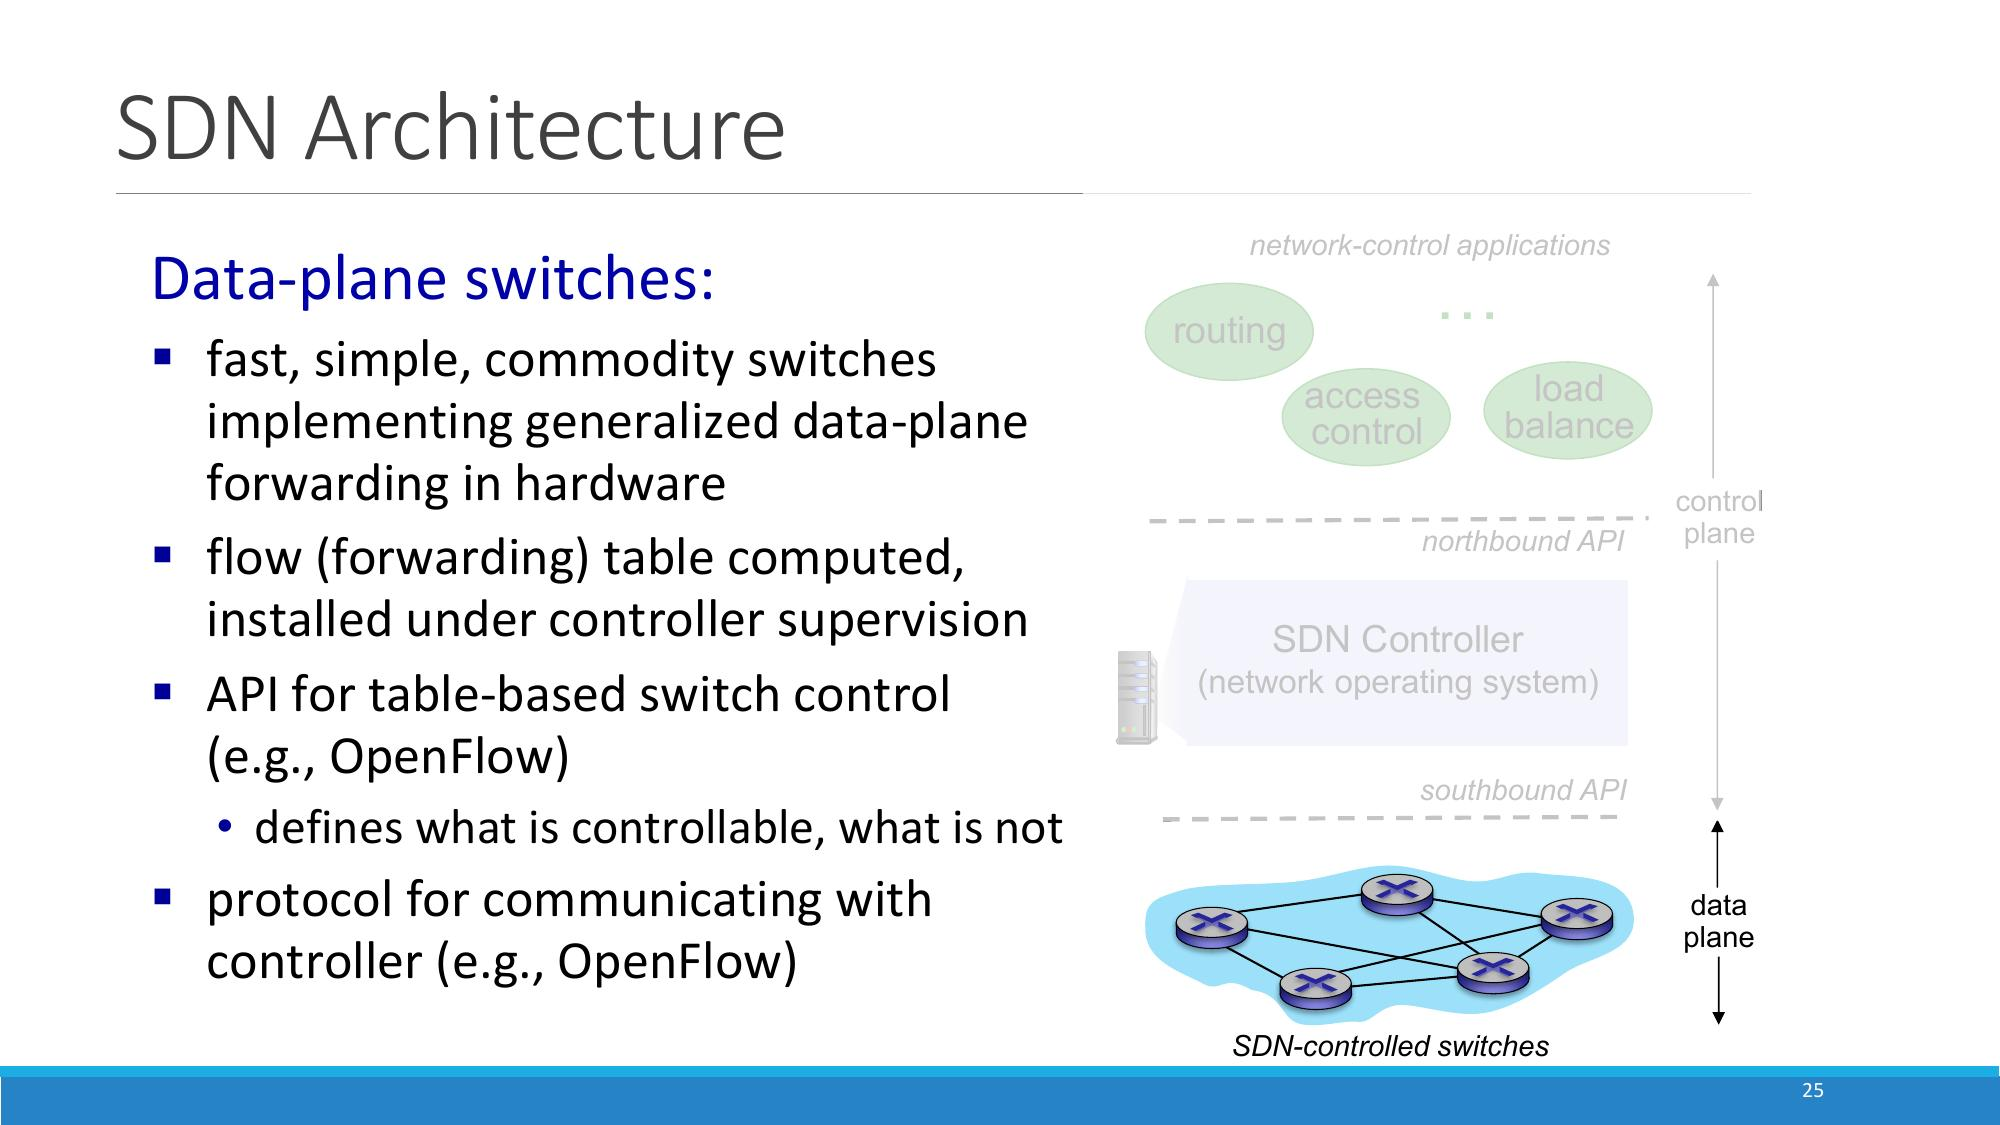
\includegraphics[keepaspectratio]{images/lezione-15-lab-sdn-architecture-img-04.jpg}}
\caption{4 --- L'architettura SDN a tre livelli.}
\end{figure}

\begin{enumerate}
\def\labelenumi{\arabic{enumi}.}
\tightlist
\item
  \textbf{Data-plane switches}: dispositivi commodity che implementano
  generalized forwarding in hardware. L'API (es. OpenFlow) definisce il
  controllo.
\item
  \textbf{SDN Controller (Network OS)}: mantiene stato globale,
  interagisce via NorthBound API con le app e via SouthBound API con gli
  switch. Fisicamente distribuito per fault-tolerance.
\item
  \textbf{Network-control applications}: il ``cervello'' unbundled
  (sviluppato da terzi) che implementa routing, firewall, ecc.
\end{enumerate}

\begin{center}\rule{0.5\linewidth}{0.5pt}\end{center}

\subsection{SDN Data Plane e Astrazione
Match-Action}\label{sdn-data-plane-e-astrazione-match-action}

Il forwarding generalizzato permette che qualsiasi campo header (L2, L3,
L4) sia usato per il \textbf{match}, associandolo a un'\textbf{azione}
(forward, drop, modify, send to controller). Questa astrazione unifica
router, switch, firewall e NAT.

\begin{callouttip}{Esempi di regole OpenFlow}

- \textbf{IP Forward}: \texttt{IP\ Dst\ =\ 51.6.0.8} →
\texttt{forward(port\ 6)} - \textbf{Firewall}:
\texttt{TCP\ dst-port\ =\ 22} → \texttt{drop}

\end{callouttip}

\subsubsection{OpenFlow Switch}\label{openflow-switch}

Uno switch OpenFlow comunica col controller via un canale sicuro
(OpenFlow Channel) e processa pacchetti usando \textbf{Flow Tables}
organizzate in \textbf{Pipeline}.
\[ \text{Packet in} \rightarrow [\text{Table 0}] \rightarrow [\text{Table 1}] \rightarrow \cdots \rightarrow [\text{Table N}] \rightarrow \text{Packet out} \]
Se non c'è match, la \emph{table-miss entry} può redirigere al
controller. Le \textbf{Group Tables} permettono azioni su più porte
(multicast/ALL, load balancing/SELECT).

\begin{figure}
\centering
\pandocbounded{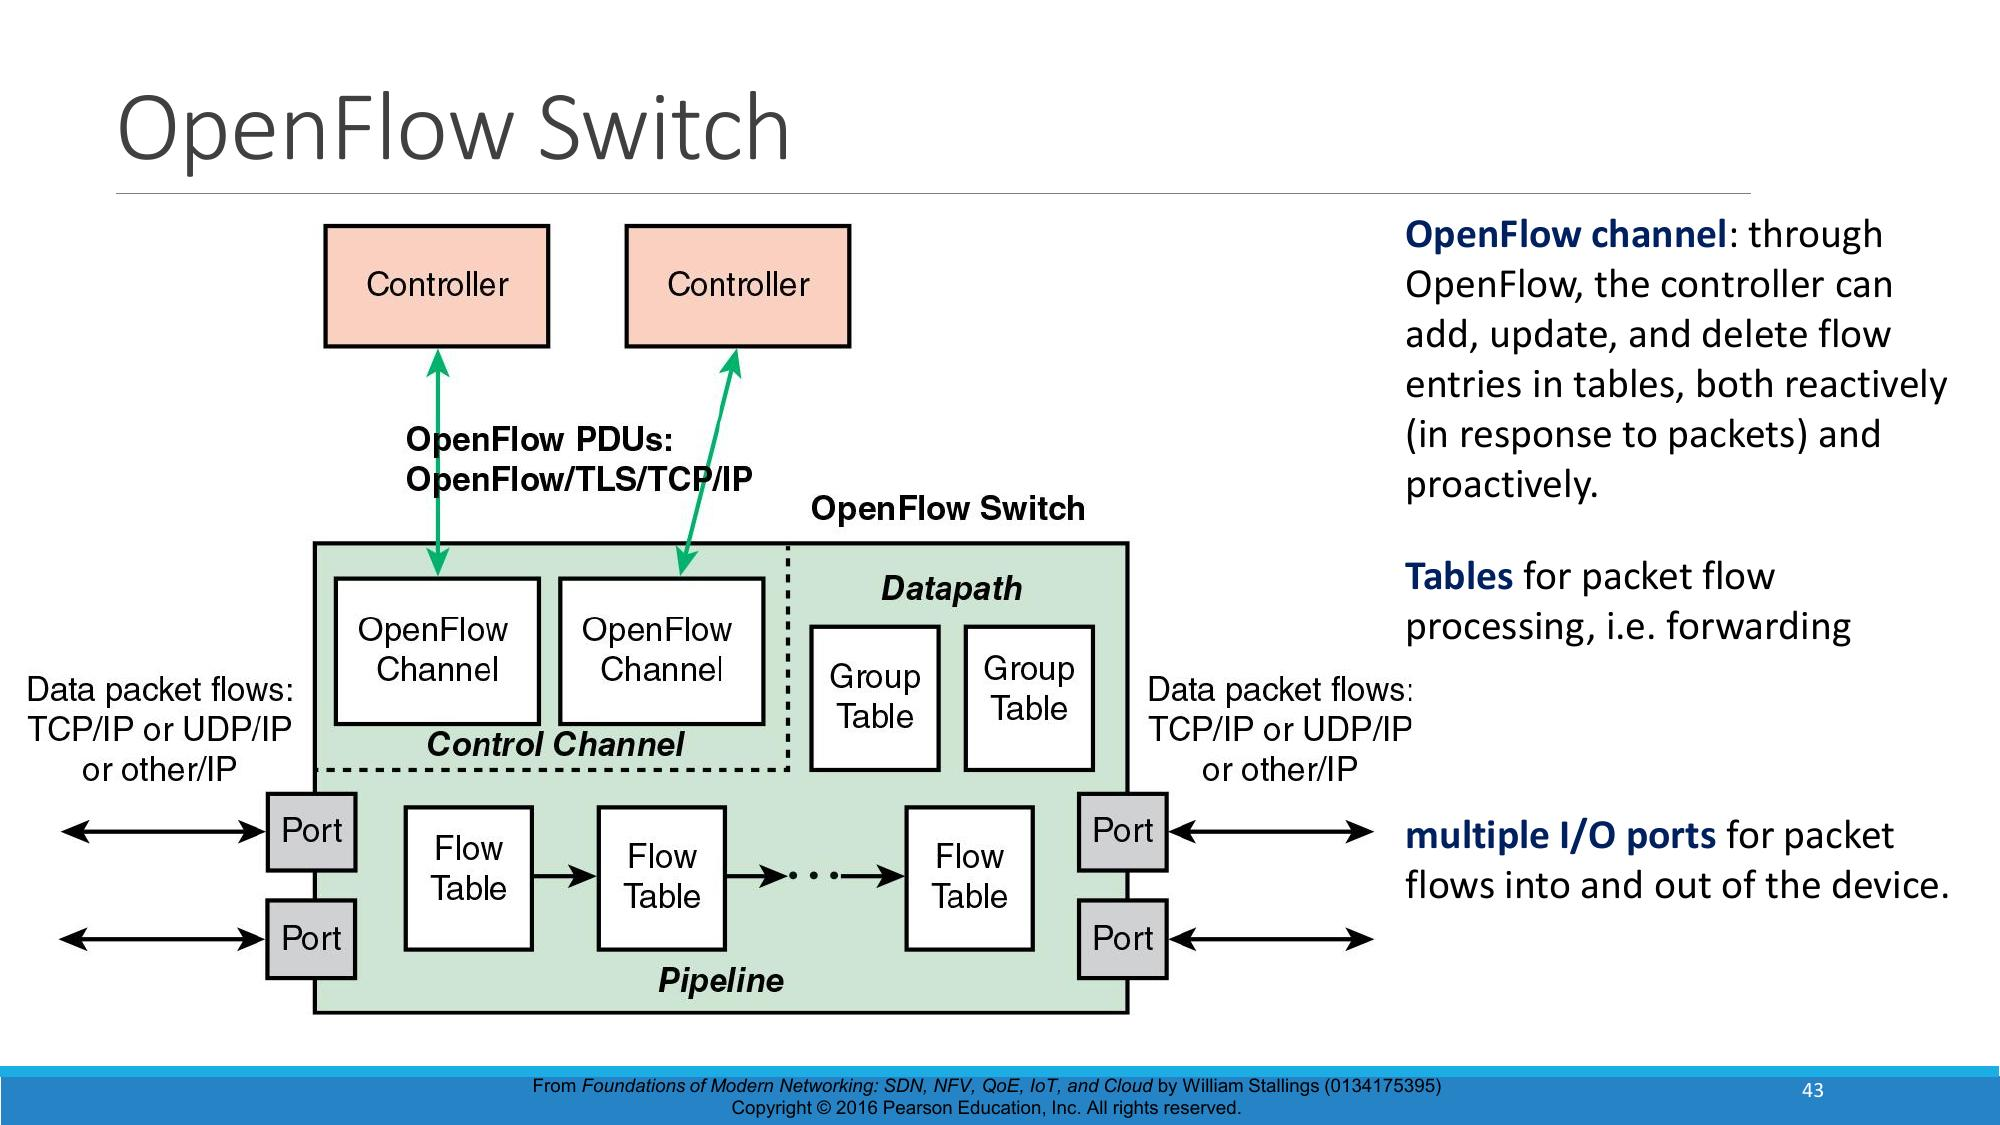
\includegraphics[keepaspectratio]{images/lezione-15-lab-sdn-architecture-img-06.jpg}}
\caption{5 --- L'OpenFlow Switch.}
\end{figure}

\begin{center}\rule{0.5\linewidth}{0.5pt}\end{center}

\subsection{SDN Control Plane}\label{sdn-control-plane}

Il controller gestisce lo stato di rete, comunica via OpenFlow e offre
astrazioni (es. SAL in OpenDaylight o Intent Framework in ONOS).
Messaggi principali di OpenFlow: \texttt{features}, \texttt{configure},
\texttt{modify-state\ (FlowMod)}, \texttt{packet-out}
(Controller→Switch) e \texttt{packet-in}, \texttt{flow-removed},
\texttt{port-status} (Switch→Controller).

\subsubsection{Path Computation e Topology
Discovery}\label{path-computation-e-topology-discovery}

Inizialmente le table sono vuote. Al primo pacchetto
(\emph{table-miss}), lo switch invia un \texttt{Packet-In}. Il
controller calcola il percorso e usa \texttt{FlowMod} per installare
regole procedendo \textbf{in ordine inverso} dalla destinazione alla
sorgente.

\begin{figure}
\centering
\pandocbounded{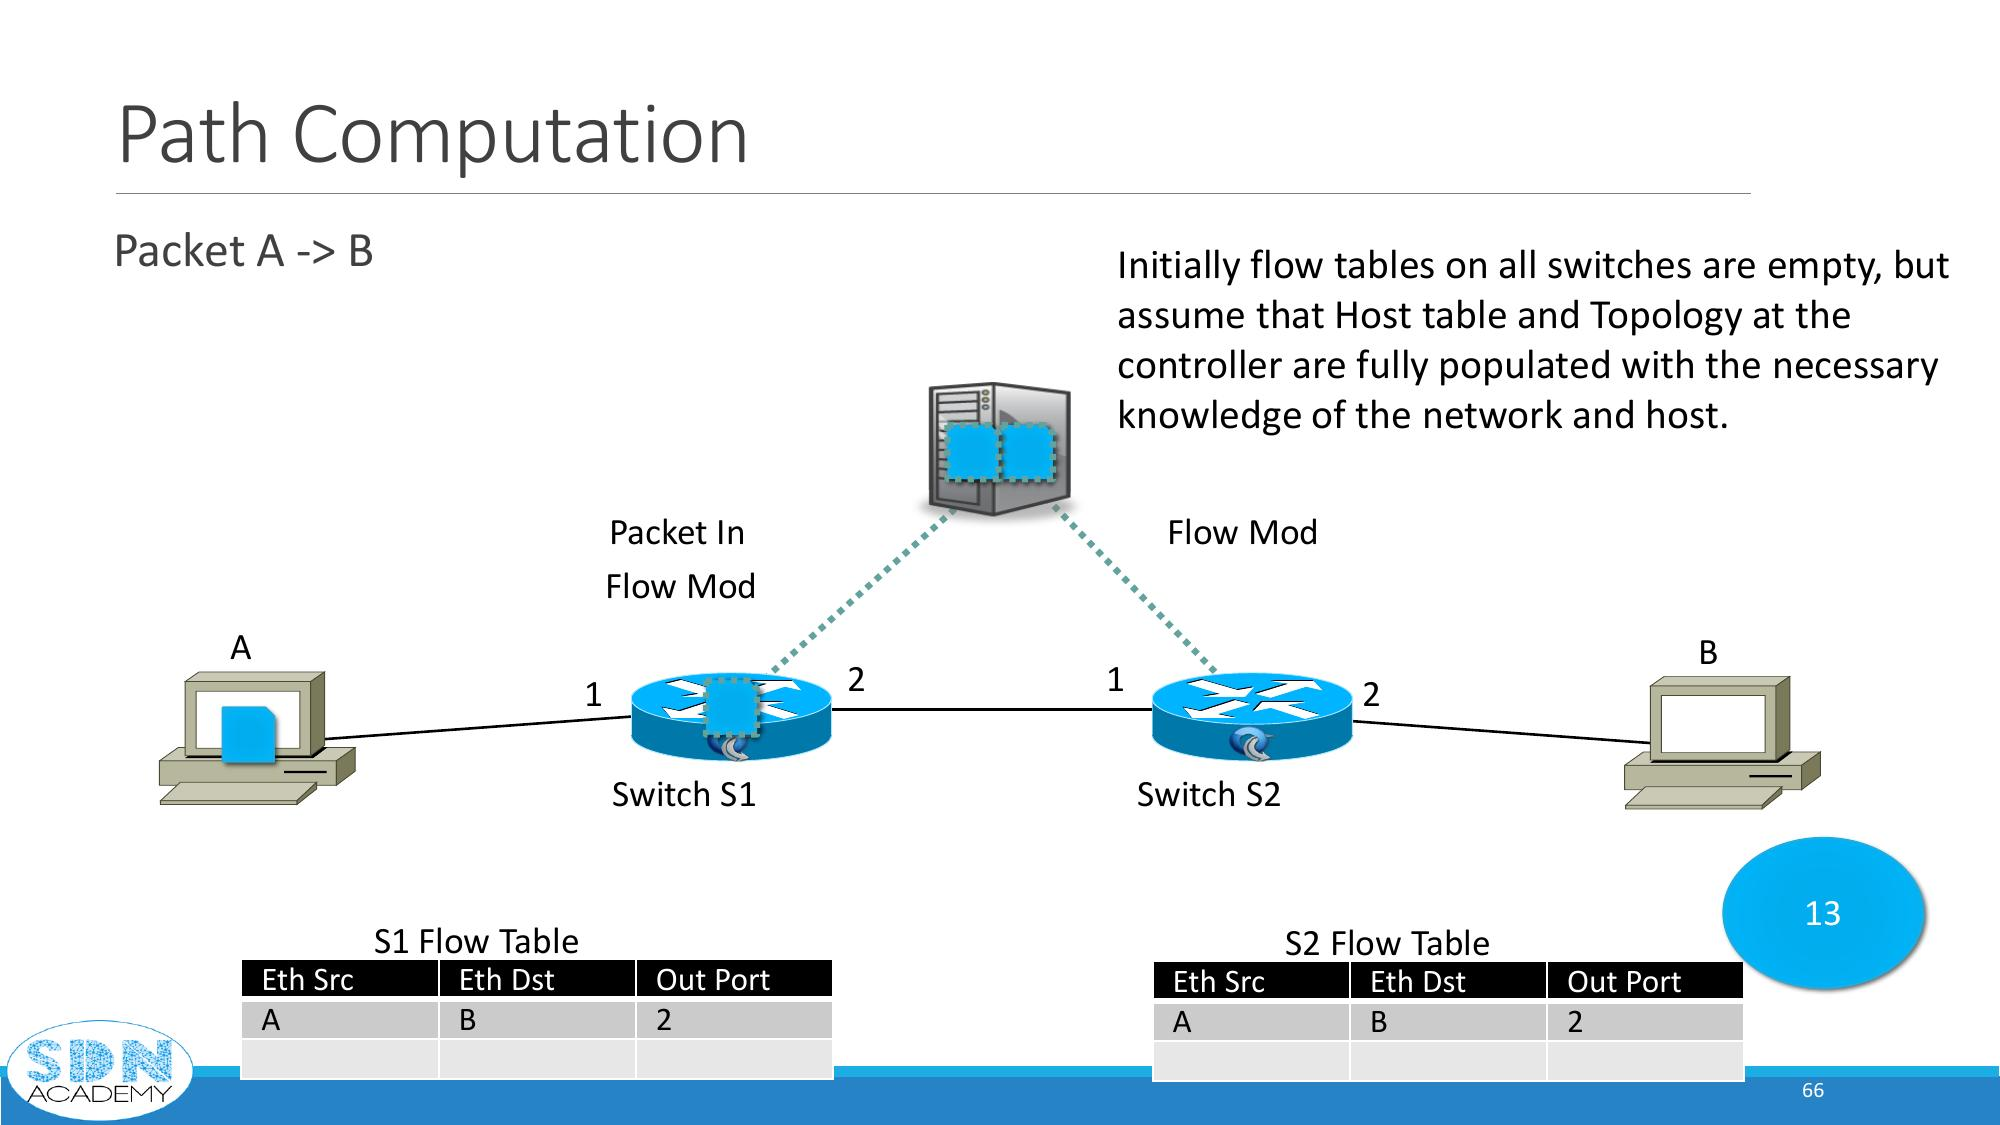
\includegraphics[keepaspectratio]{images/lezione-15-lab-sdn-architecture-img-07.jpg}}
\caption{6 --- Path computation reattiva.}
\end{figure}

Al boot, avviene l'\textbf{Inizializzazione} con scambio Feature
Request/Reply. Poi, la topologia viene scoperta tramite \textbf{LLDP}
(Link Layer Discovery Protocol, \texttt{0x88cc}). 1. Il controller invia
\emph{Packet-Out} con LLDP. 2. Lo switch forwarda. 3. Lo switch
adiacente riceve e manda \emph{Packet-In} al controller con metadati. Il
controller deduce i link fisici.

\begin{figure}
\centering
\pandocbounded{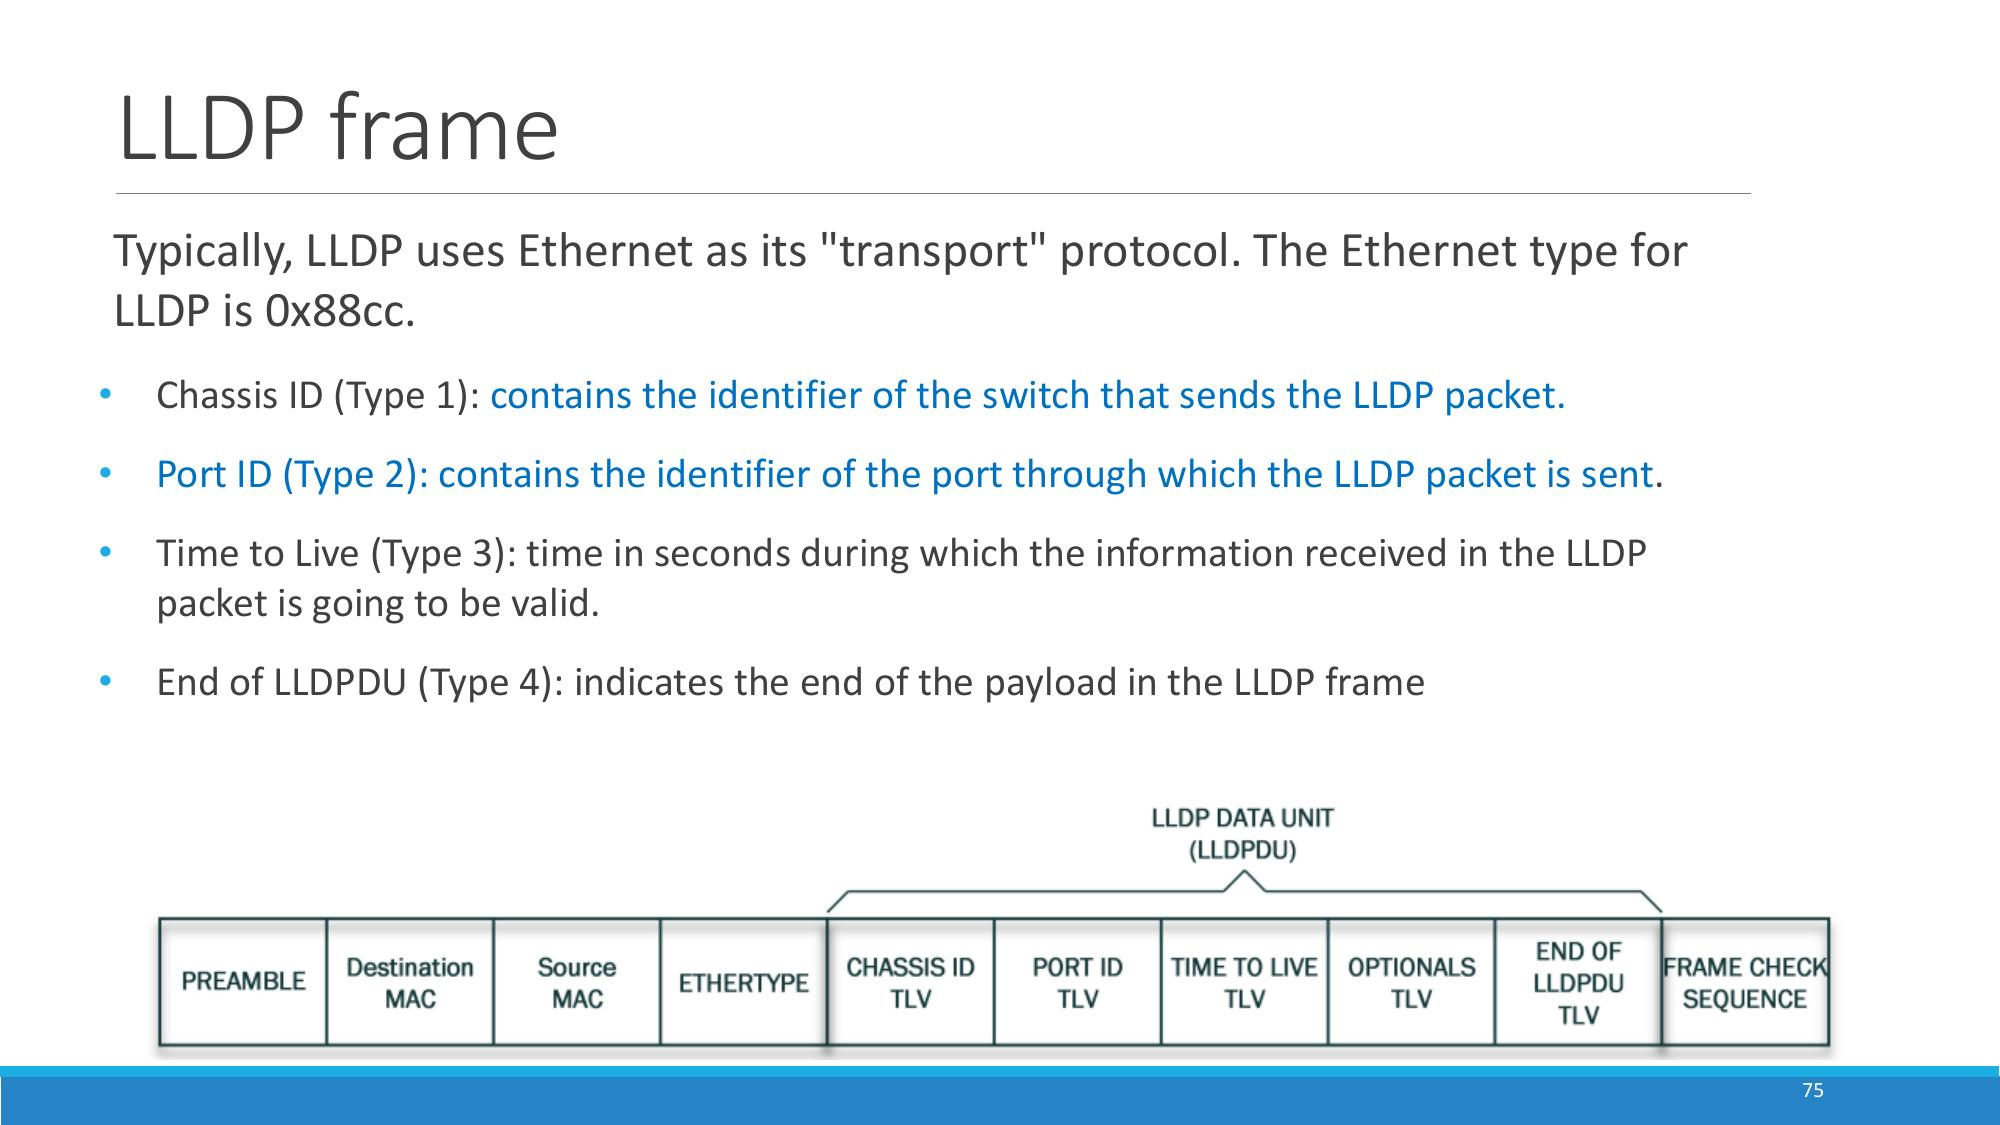
\includegraphics[keepaspectratio]{images/lezione-15-lab-sdn-architecture-img-09.jpg}}
\caption{7 --- Struttura del frame LLDP.}
\end{figure}

\begin{center}\rule{0.5\linewidth}{0.5pt}\end{center}

\section{2. SDN Applications e P4
Language}\label{sdn-applications-e-p4-language}

\subsection{B4: La WAN SDN di Google}\label{b4-la-wan-sdn-di-google}

Le WAN tradizionali hanno link costosi sottoutilizzati (30-40\%) a causa
dell'overprovisioning. \textbf{B4} è la rete inter-datacenter SDN di
Google che ottimizza il traffico ``bulk'' elastico (replicazioni) per
avvicinarsi al 100\% di utilizzo.

\begin{figure}
\centering
\pandocbounded{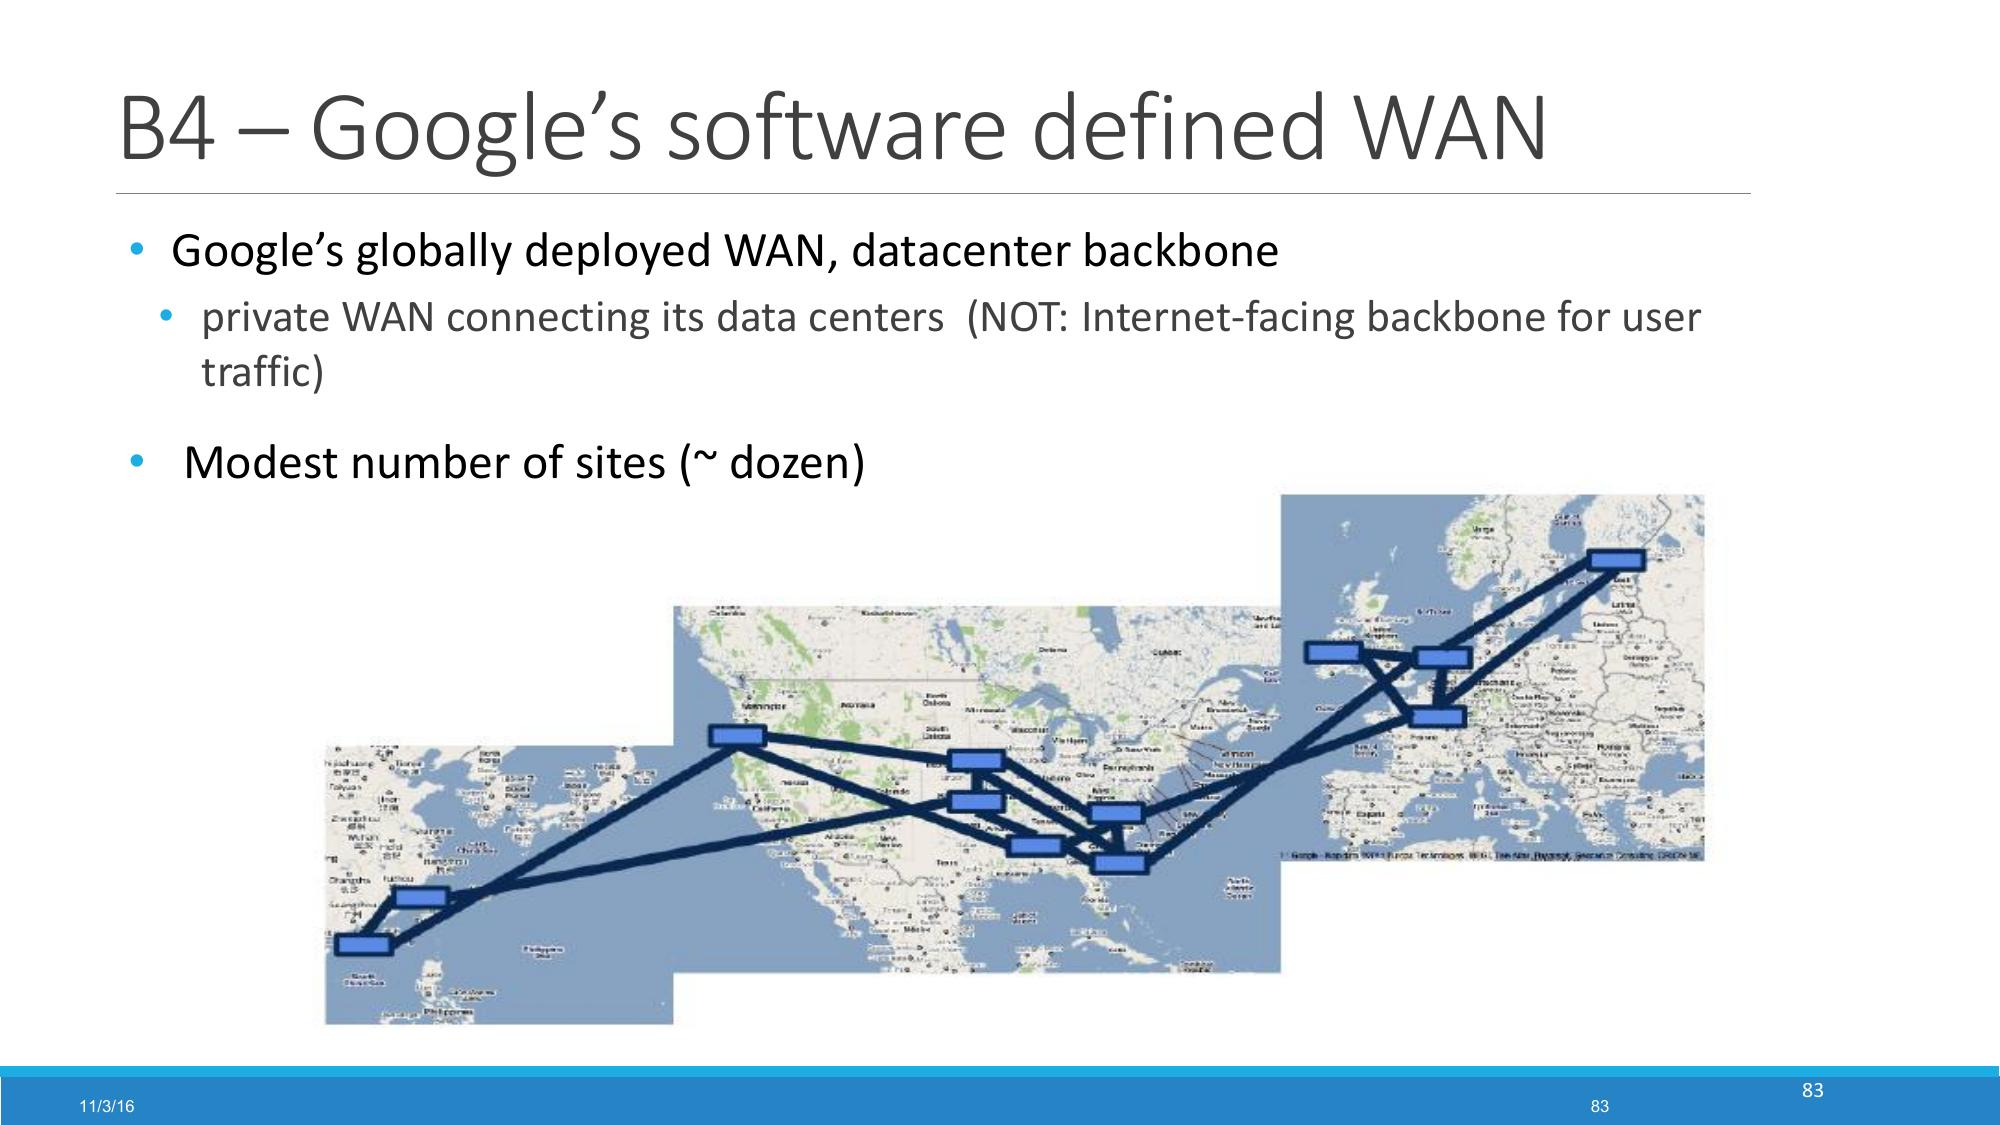
\includegraphics[keepaspectratio]{images/lezione-16-lab-sdn-applications-e-p4-language-img-01.jpg}}
\caption{8 --- La rete B4 mondiale.}
\end{figure}

La migrazione è avvenuta a stadi, mantenendo \textbf{BGP} per la
raggiungibilità di base ma delegando al \textbf{Central TE Server} (SDN)
l'ottimizzazione del traffico e il routing tramite \textbf{forwarding
multipath} su Tunnel logici IP-in-IP.

\begin{figure}
\centering
\pandocbounded{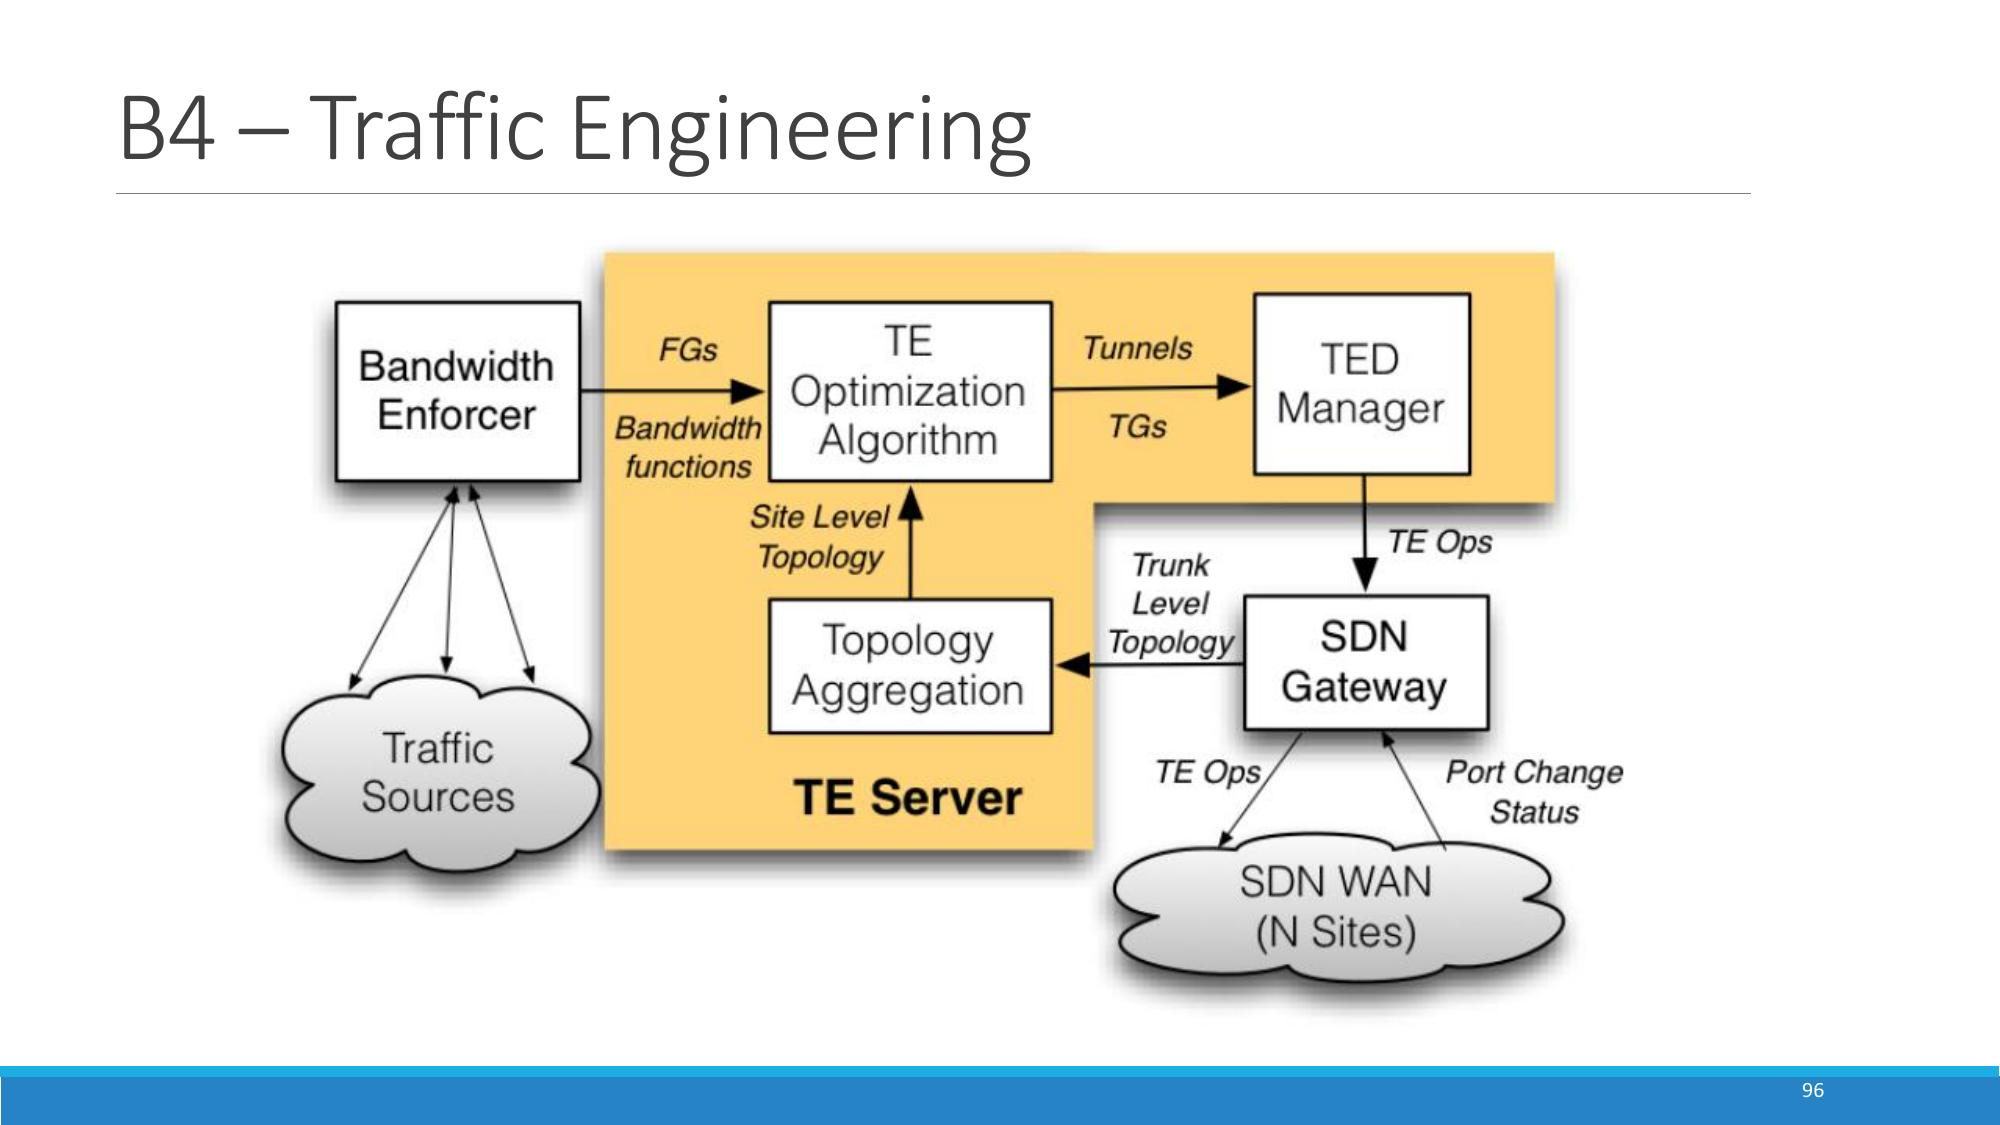
\includegraphics[keepaspectratio]{images/lezione-16-lab-sdn-applications-e-p4-language-img-07.jpg}}
\caption{9 --- Il TE Server riceve Flow Groups e installa Tunnels
tramite controller OpenFlow.}
\end{figure}

\subsection{Il Linguaggio P4}\label{il-linguaggio-p4}

OpenFlow ha il limite di proporre tabelle hardware rigide. \textbf{P4}
(\emph{Programming Protocol-Independent Packet Processors}) permette di
\textbf{programmare il data plane}, definendo header e tabelle stesse.

Un programma P4 contiene: 1. \textbf{Parser}: macchina a stati per
estrarre header. 2. \textbf{Match-Action Pipeline}: logica definita dal
programmatore. 3. \textbf{Deparser}: serializzazione.

\begin{figure}
\centering
\pandocbounded{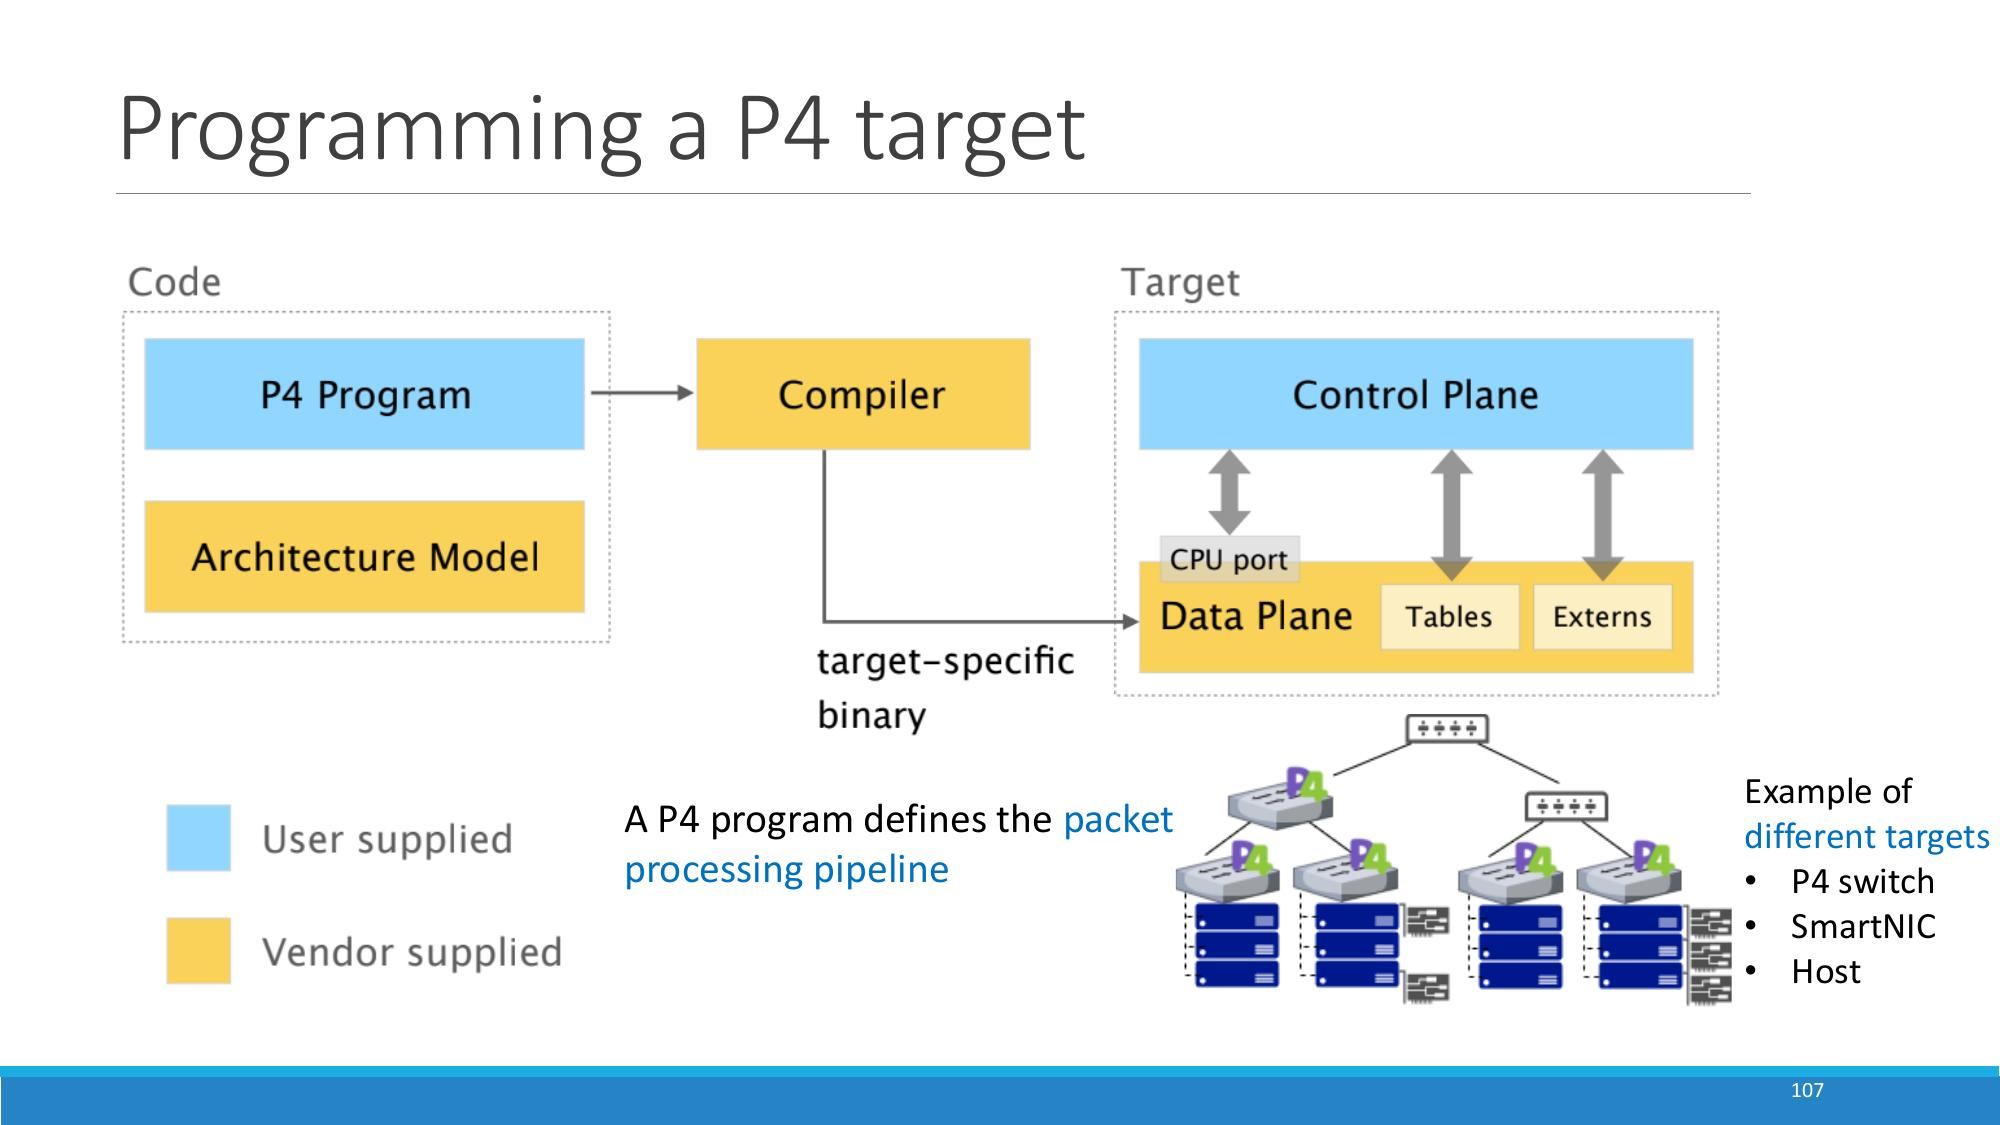
\includegraphics[keepaspectratio]{images/lezione-16-lab-sdn-applications-e-p4-language-img-09.jpg}}
\caption{10 --- Compilazione P4 verso target diversi, interagendo con
P4Runtime.}
\end{figure}

\begin{Shaded}
\begin{Highlighting}[]
\NormalTok{parser MyParser(packet\_in packet, out headers\_t hdr, inout metadata\_t meta) \{}
\NormalTok{    state start \{}
\NormalTok{        packet.extract(hdr.ethernet);}
\NormalTok{        transition select(hdr.ethernet.eth\_type) \{}
\NormalTok{            0x0800: parse\_ipv4;}
\NormalTok{            default: accept;}
\NormalTok{        \}}
\NormalTok{    \}}
\NormalTok{    state parse\_ipv4 \{ packet.extract(hdr.ipv4); transition accept; \}}
\NormalTok{\}}
\end{Highlighting}
\end{Shaded}

\subsection{Service Function Chaining
(SFC)}\label{service-function-chaining-sfc}

Comporre funzioni (Firewall, IDS) senza ricablare la rete fisica. SDN
permette definizioni logiche dinamiche, deviando il traffico tramite
\emph{Service Classifiers}.

\begin{figure}
\centering
\pandocbounded{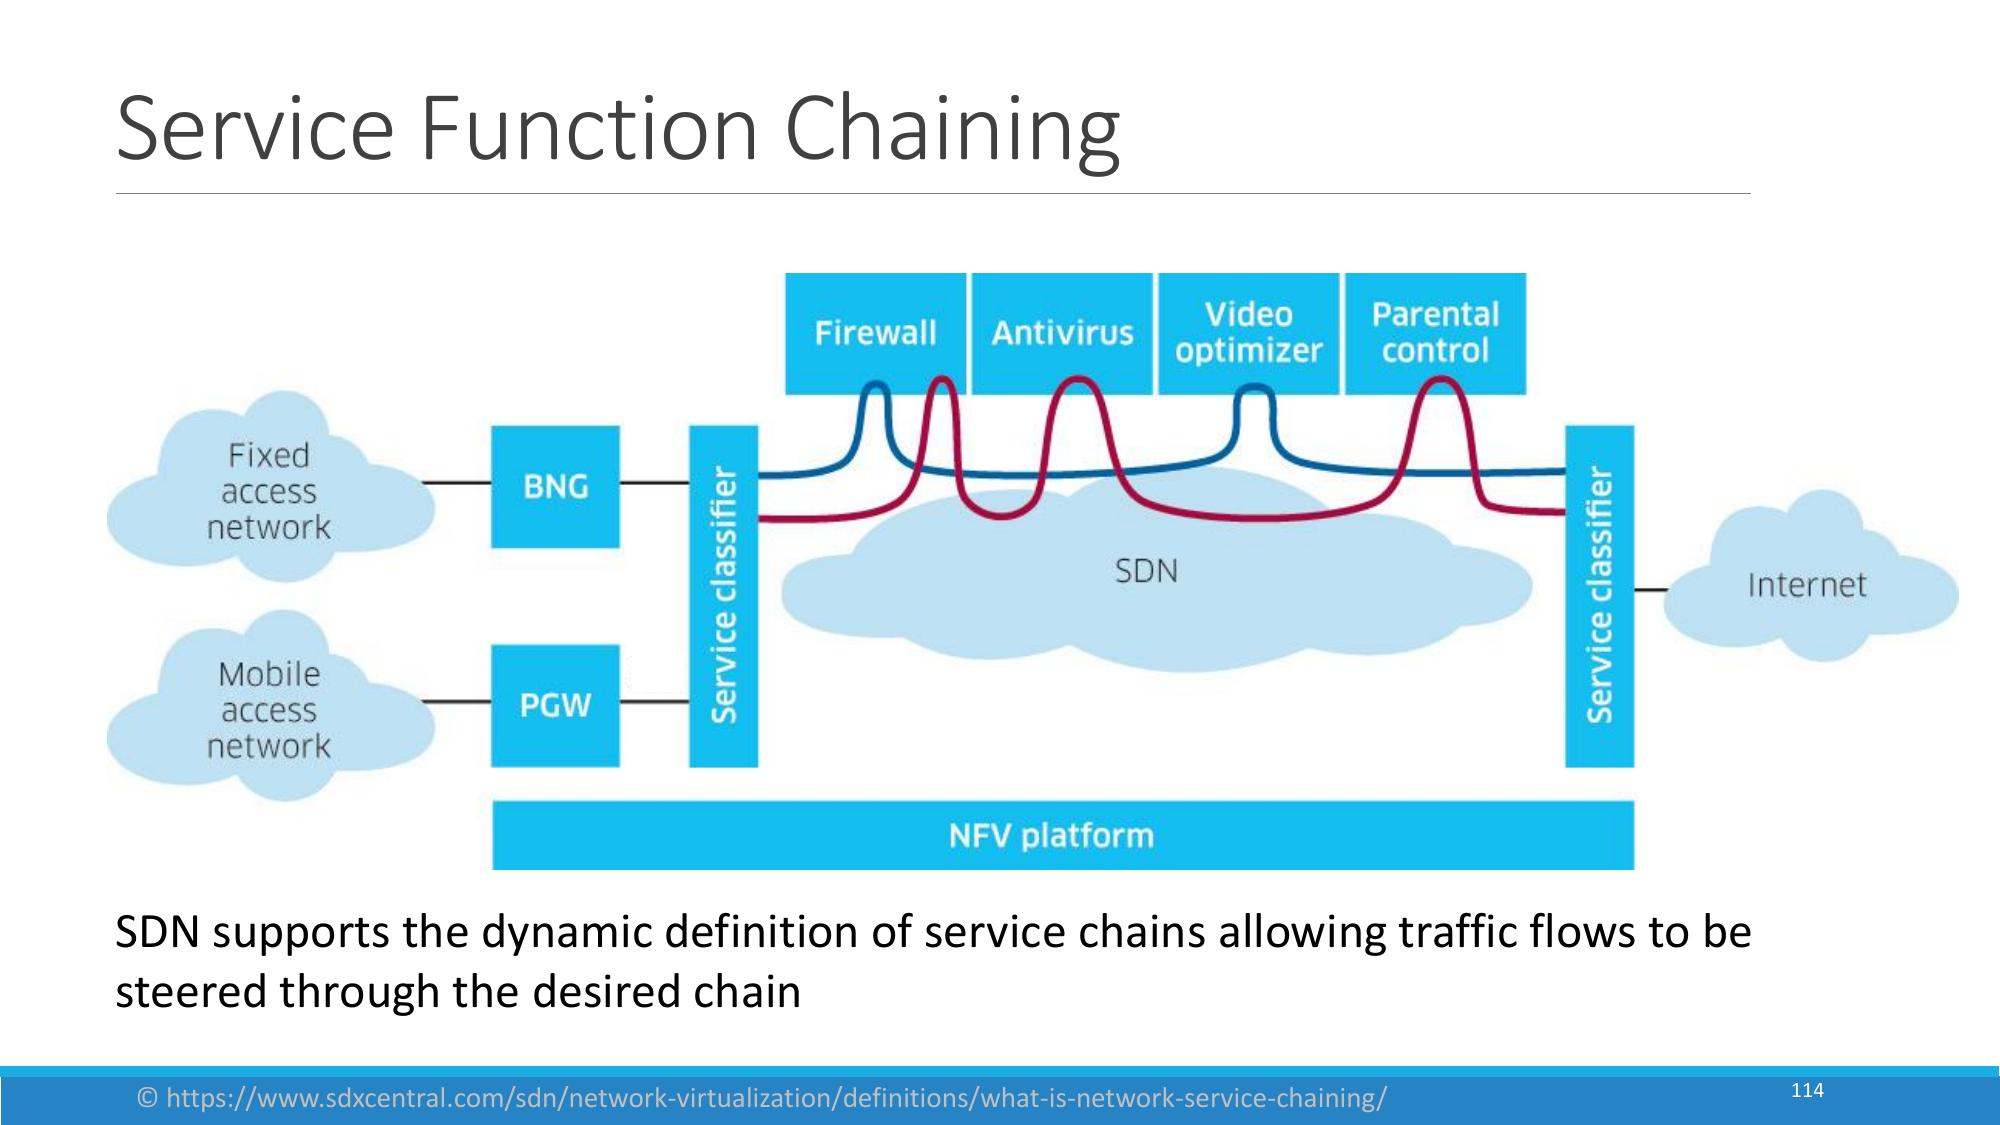
\includegraphics[keepaspectratio]{images/lezione-16-lab-sdn-applications-e-p4-language-img-11.jpg}}
\caption{11 --- Service Function Chaining.}
\end{figure}

\begin{center}\rule{0.5\linewidth}{0.5pt}\end{center}

\section{3. Network Function Virtualization
(NFV)}\label{network-function-virtualization-nfv}

\subsection{Dal Middlebox all'Appliance
Software}\label{dal-middlebox-allappliance-software}

I middlebox hardware (Firewall, NAT) rendono rigida la rete.
\textbf{NFV} si basa sul \textbf{decoupling} (disaccoppiamento) tra
funzioni e hardware proprietario, trasformandole in \textbf{VNF}
(\emph{Virtualized Network Function}) in esecuzione su server commodity
(COTS) come Macchine Virtuali (VM) o Container (CNF).

\begin{figure}
\centering
\pandocbounded{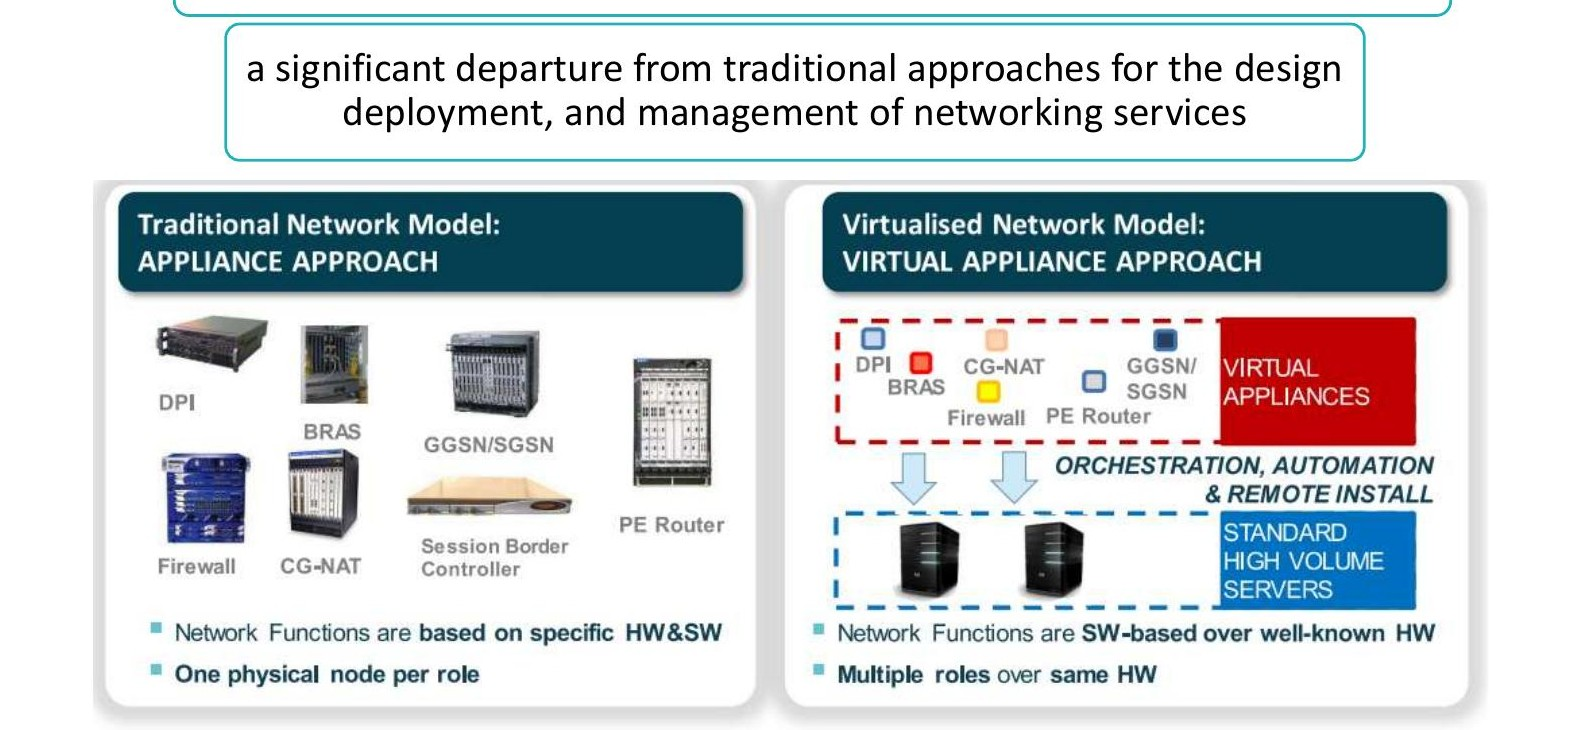
\includegraphics[keepaspectratio]{images/lezione-20-lab-network-function-virtualization-img-01.jpg}}
\caption{\emph{Fig. 12 --- Modello tradizionale vs NFV.} Benefici:
Flessibilità, Scalabilità elastica (scaling up/down), Innovazione
rapida.}
\end{figure}

\subsection{Network Function Forwarding Graph
(NF-FG)}\label{network-function-forwarding-graph-nf-fg}

Un servizio end-to-end è un grafo logico (VNF-FG) composto da VNF
connesse da link virtuali, che l'orchestratore mappa su reti
infrastrutturali (\emph{NFVI-PoP}). Il problema del \emph{VNF Placement}
consiste nel trovare l'allocazione ottima per ridurre latenza ed
overhead.

\begin{figure}
\centering
\pandocbounded{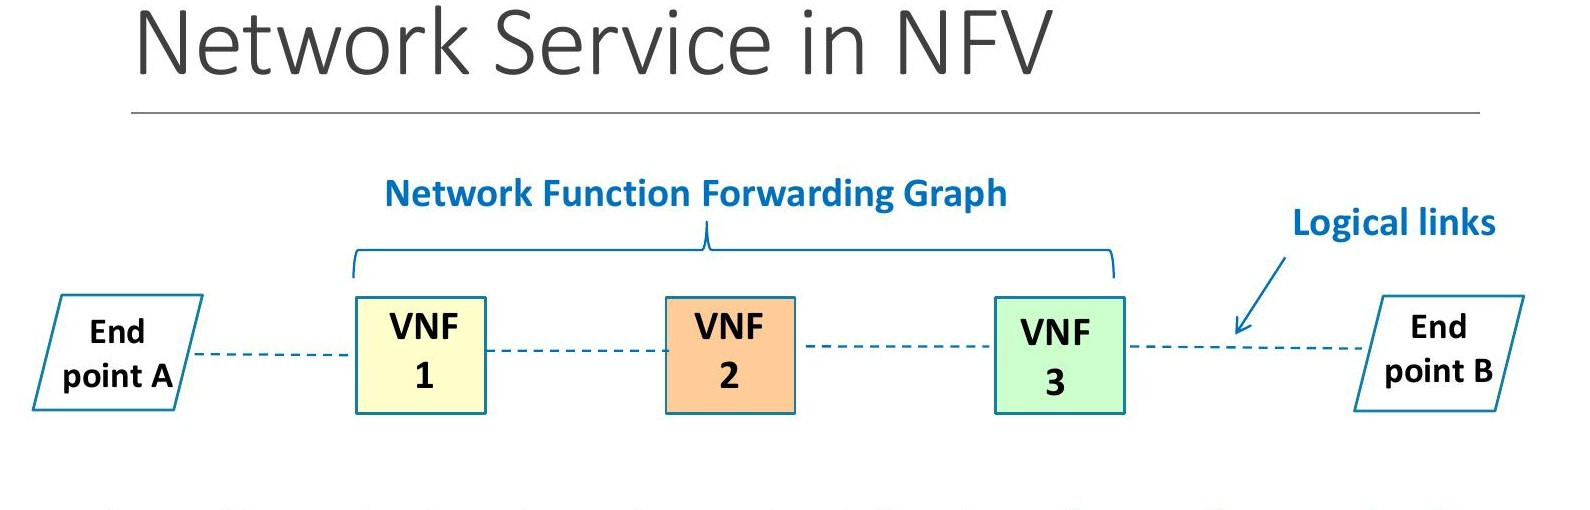
\includegraphics[keepaspectratio]{images/lezione-20-lab-network-function-virtualization-img-04.jpg}}
\caption{13 --- VNF-FG.}
\end{figure}

\subsection{Architettura ETSI
NFV-MANO}\label{architettura-etsi-nfv-mano}

\begin{figure}
\centering
\pandocbounded{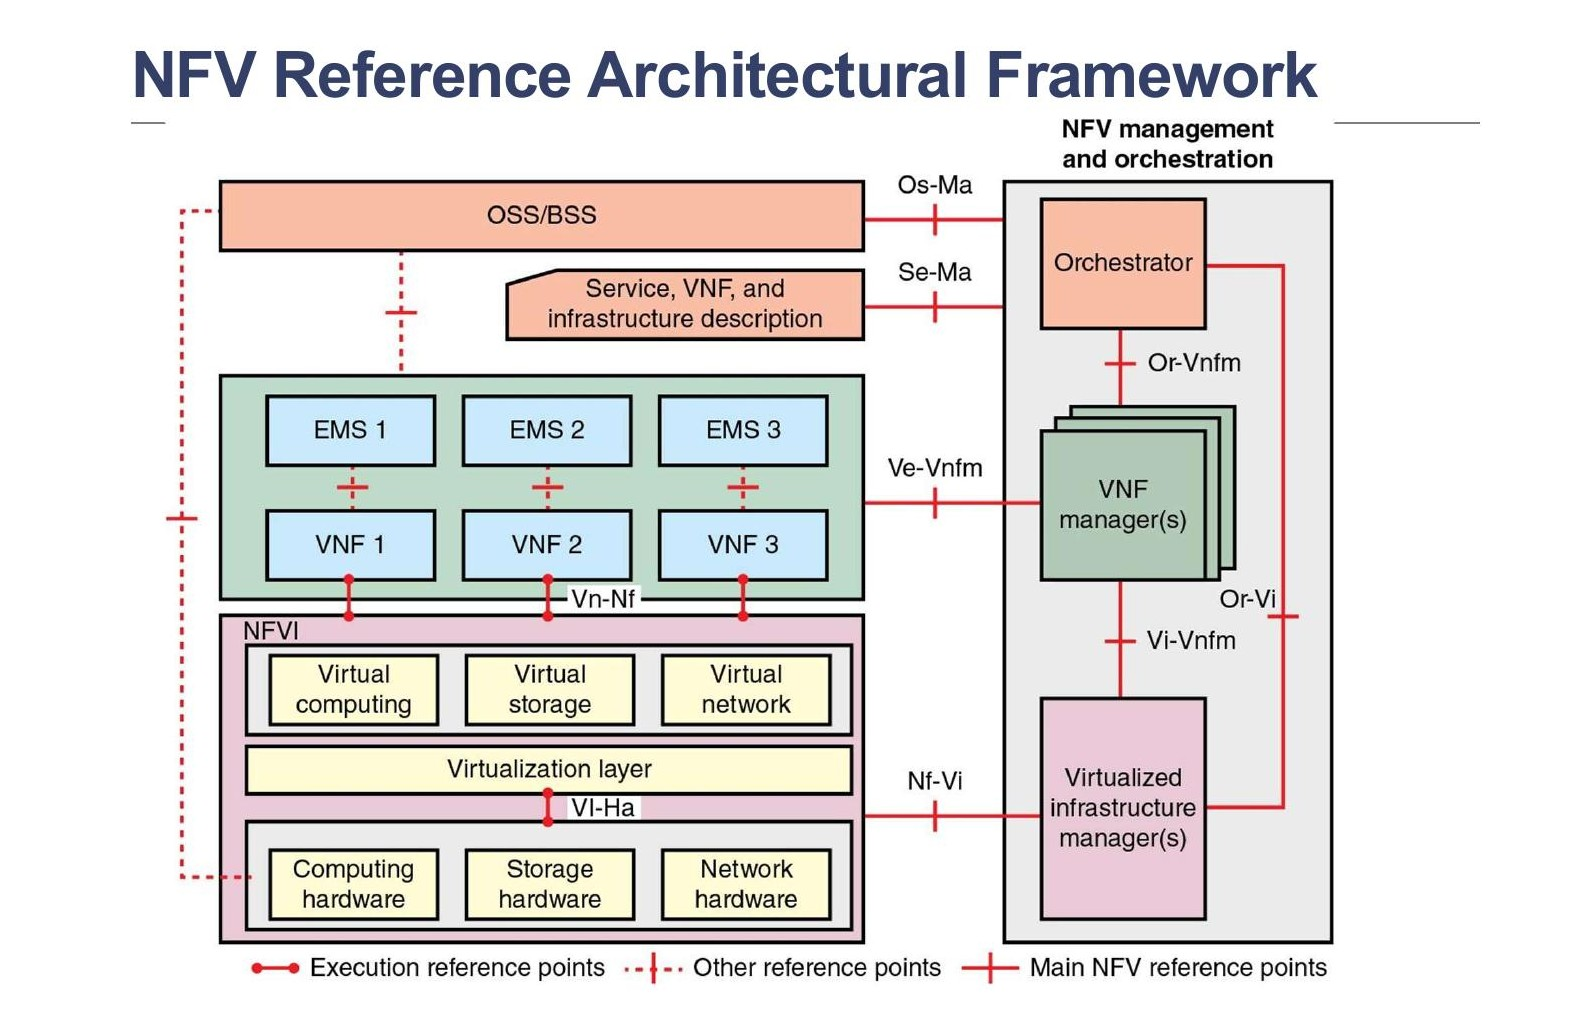
\includegraphics[keepaspectratio]{images/lezione-20-lab-network-function-virtualization-img-07.jpg}}
\caption{14 --- Architettura di riferimento NFV.}
\end{figure}

L'infrastruttura è tripartita: 1. \textbf{NFVI} (Infrastructure):
compute, hypervisor, networking. Switch virtuali come Open vSwitch (OVS)
gestiscono le reti virtuali. 2. \textbf{VNF}: Le funzioni instanziate.
3. \textbf{NFV-MANO} (Management and Orchestration): - \textbf{NFVO}
(Orchestrator): gestisce i \emph{Network Services}. - \textbf{VNFM}
(Manager): gestisce il ciclo di vita (scaling, healing) di singole VNF.
- \textbf{VIM} (Virtualized Infrastructure Manager): gestisce l'hardware
fisico sottostante (es. OpenStack).

\begin{callouttip}{Network Service Descriptor (NSD)}

Formato (es. JSON) che definisce come le VNF compongono il servizio e i
link virtuali che le legano.

\end{callouttip}

\begin{center}\rule{0.5\linewidth}{0.5pt}\end{center}

\section{4. Emulazione con ComNetsEmu e
Mininet}\label{emulazione-con-comnetsemu-e-mininet}

\textbf{Mininet} emula host, switch e link in un solo kernel usando i
\textbf{network namespace} Linux (per l'isolamento degli stack di rete)
e interfacce \textbf{veth pairs}. \textbf{ComNetsEmu} estende Mininet
usando \emph{container Docker} per emulare host SDN/NFV
(Docker-in-Docker).

\begin{figure}
\centering
\pandocbounded{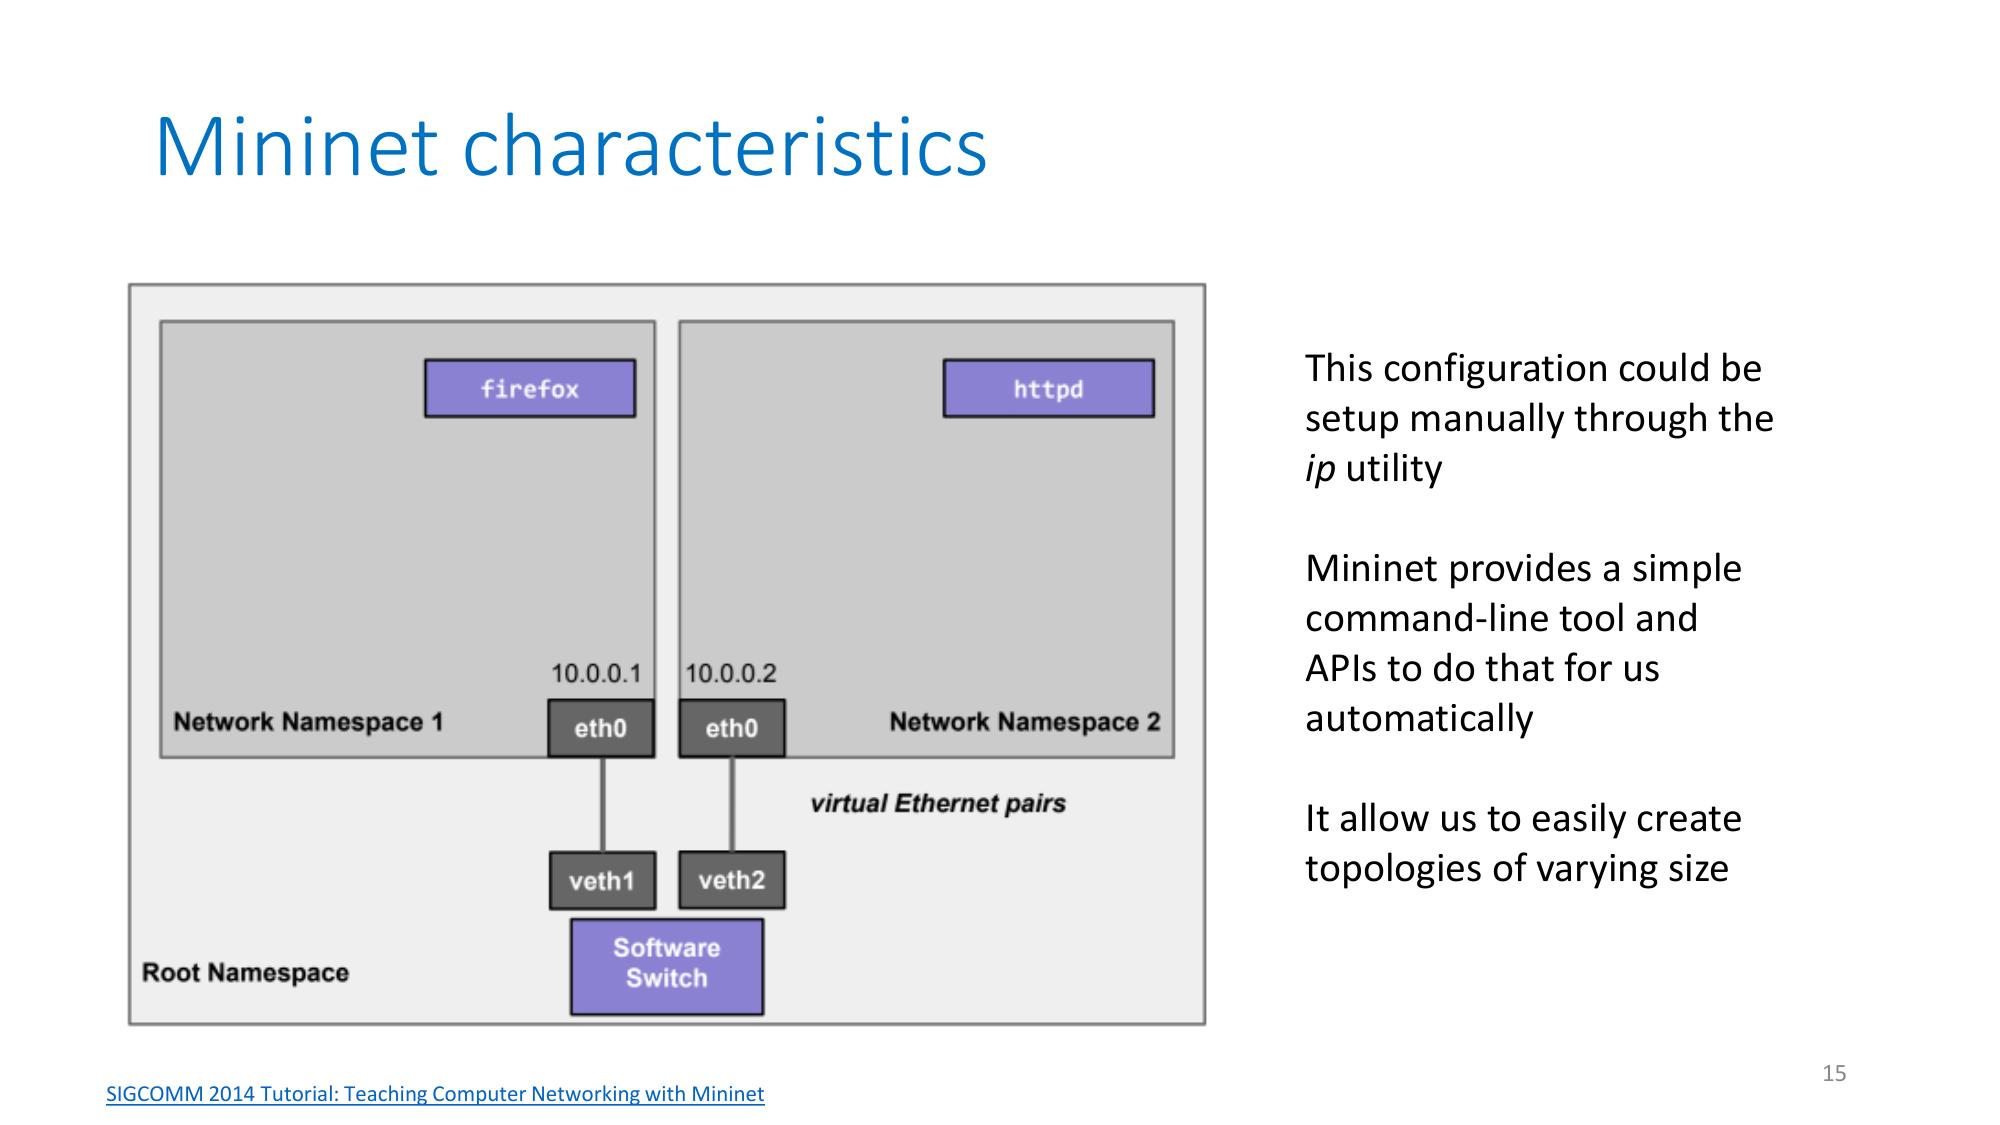
\includegraphics[keepaspectratio]{images/lezione-21-lab-network-emulator-con-comnetsemu-img-04.jpg}}
\caption{15 --- Namespace isolati in Mininet connessi via veth.}
\end{figure}

\subsection{Gestione da CLI}\label{gestione-da-cli}

I comandi Mininet e \texttt{tc} (Traffic Control) permettono test
avanzati:

\begin{Shaded}
\begin{Highlighting}[]
\ExtensionTok{mininet}\OperatorTok{\textgreater{}}\NormalTok{ h1 ping h2}
\ExtensionTok{mininet}\OperatorTok{\textgreater{}}\NormalTok{ iperf h1 h2}
\ExtensionTok{h1}\NormalTok{ tc qdisc add dev h1{-}eth0 root netem delay 100ms 10ms }\CommentTok{\# Configura ritardo}
\end{Highlighting}
\end{Shaded}

\subsection{Esempio: Echo Server in
Python}\label{esempio-echo-server-in-python}

Topologia con due host Docker: \texttt{h1} (bash client) e \texttt{h2}
(echo\_server).

\begin{Shaded}
\begin{Highlighting}[]
\OperatorTok{**}\NormalTok{topology.py (Estratto)}\OperatorTok{**}
\NormalTok{h1 }\OperatorTok{=}\NormalTok{ net.addDockerHost(}\StringTok{"h1"}\NormalTok{, dimage}\OperatorTok{=}\StringTok{"dev\_test"}\NormalTok{, ip}\OperatorTok{=}\StringTok{"10.0.0.1"}\NormalTok{)}
\NormalTok{h2 }\OperatorTok{=}\NormalTok{ net.addDockerHost(}\StringTok{"h2"}\NormalTok{, dimage}\OperatorTok{=}\StringTok{"echo\_server"}\NormalTok{, ip}\OperatorTok{=}\StringTok{"10.0.0.2"}\NormalTok{)}
\NormalTok{net.addLink(switch1, h1, bw}\OperatorTok{=}\DecValTok{10}\NormalTok{, delay}\OperatorTok{=}\StringTok{"10ms"}\NormalTok{)}
\end{Highlighting}
\end{Shaded}

Server testabile con Netcat:

\begin{Shaded}
\begin{Highlighting}[]
\ExtensionTok{h1:/\#}\NormalTok{ nc 10.0.0.2 65000}
\end{Highlighting}
\end{Shaded}

\begin{center}\rule{0.5\linewidth}{0.5pt}\end{center}

\section{5. Multi-Access Edge Computing
(MEC)}\label{multi-access-edge-computing-mec}

MEC porta le risorse elaborative ai margini (Edge) per avvicinarle
all'utente finale (Base Station, Access Point, micro-data center).
Questo approccio ottimizza la \textbf{Formula di Mathis} per il
throughput TCP, che dipende inversamente dal Round Trip Time (\(RTT\)) e
dalla perdita di pacchetti (\(P_{loss}\)).
\[ \text{Throughput} \le \frac{MSS}{RTT \sqrt{P_{loss}}} \]

\begin{figure}
\centering
\pandocbounded{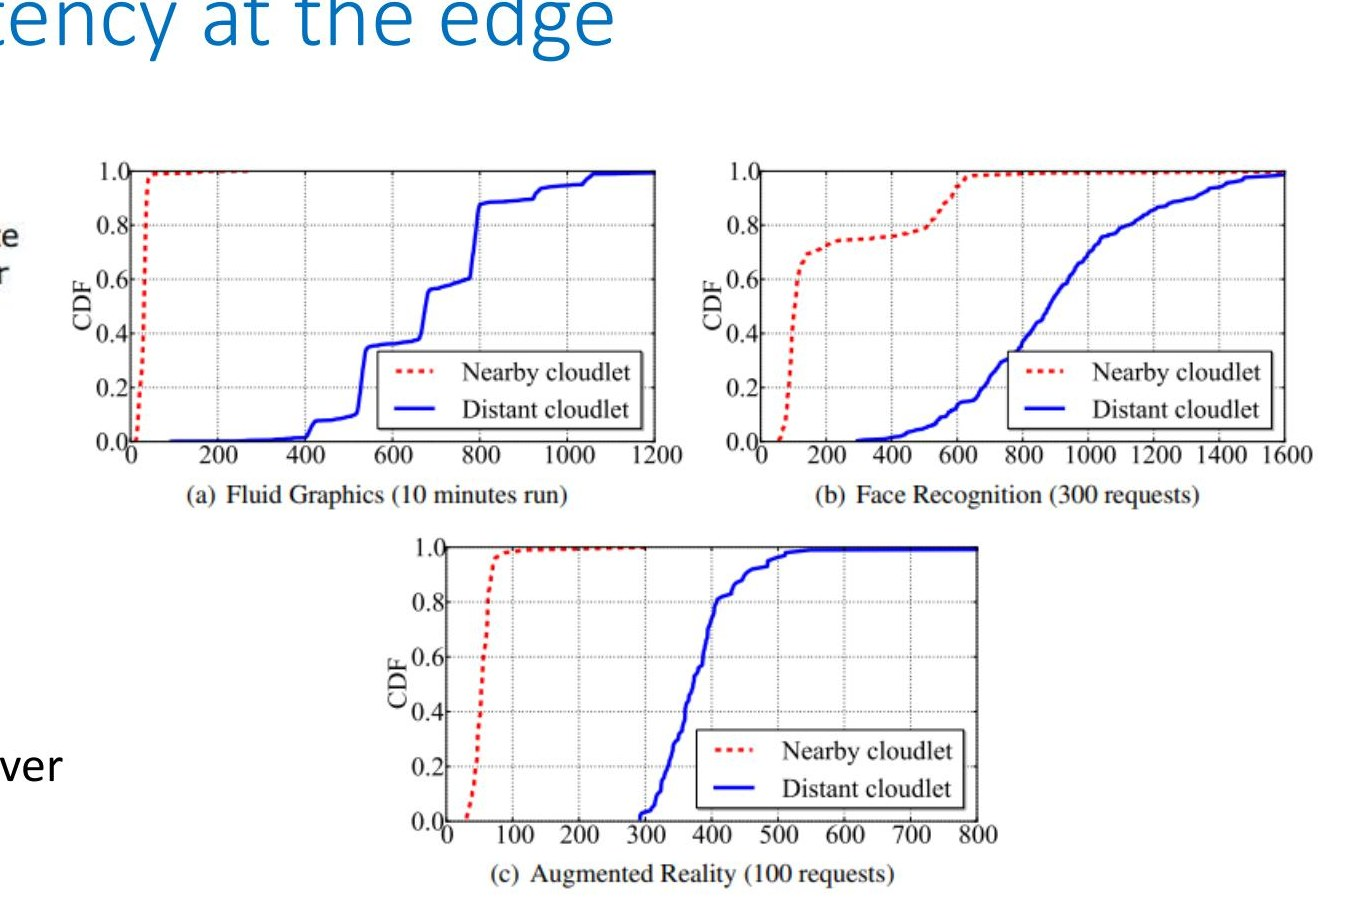
\includegraphics[keepaspectratio]{images/lezione-22-lab-multi-access-edge-computing-mec-img-02.jpg}}
\caption{16 --- CDF: La prossimità (cloudlet vicino) abbatte
sensibilmente la latenza.}
\end{figure}

\subsection{Benefici e Scenari}\label{benefici-e-scenari}

Oltre al calo di latenza, MEC supporta video analytics locali (non
saturando la WAN), funziona da IoT Gateway intelligente e facilita le
garanzie privacy.

\begin{figure}
\centering
\pandocbounded{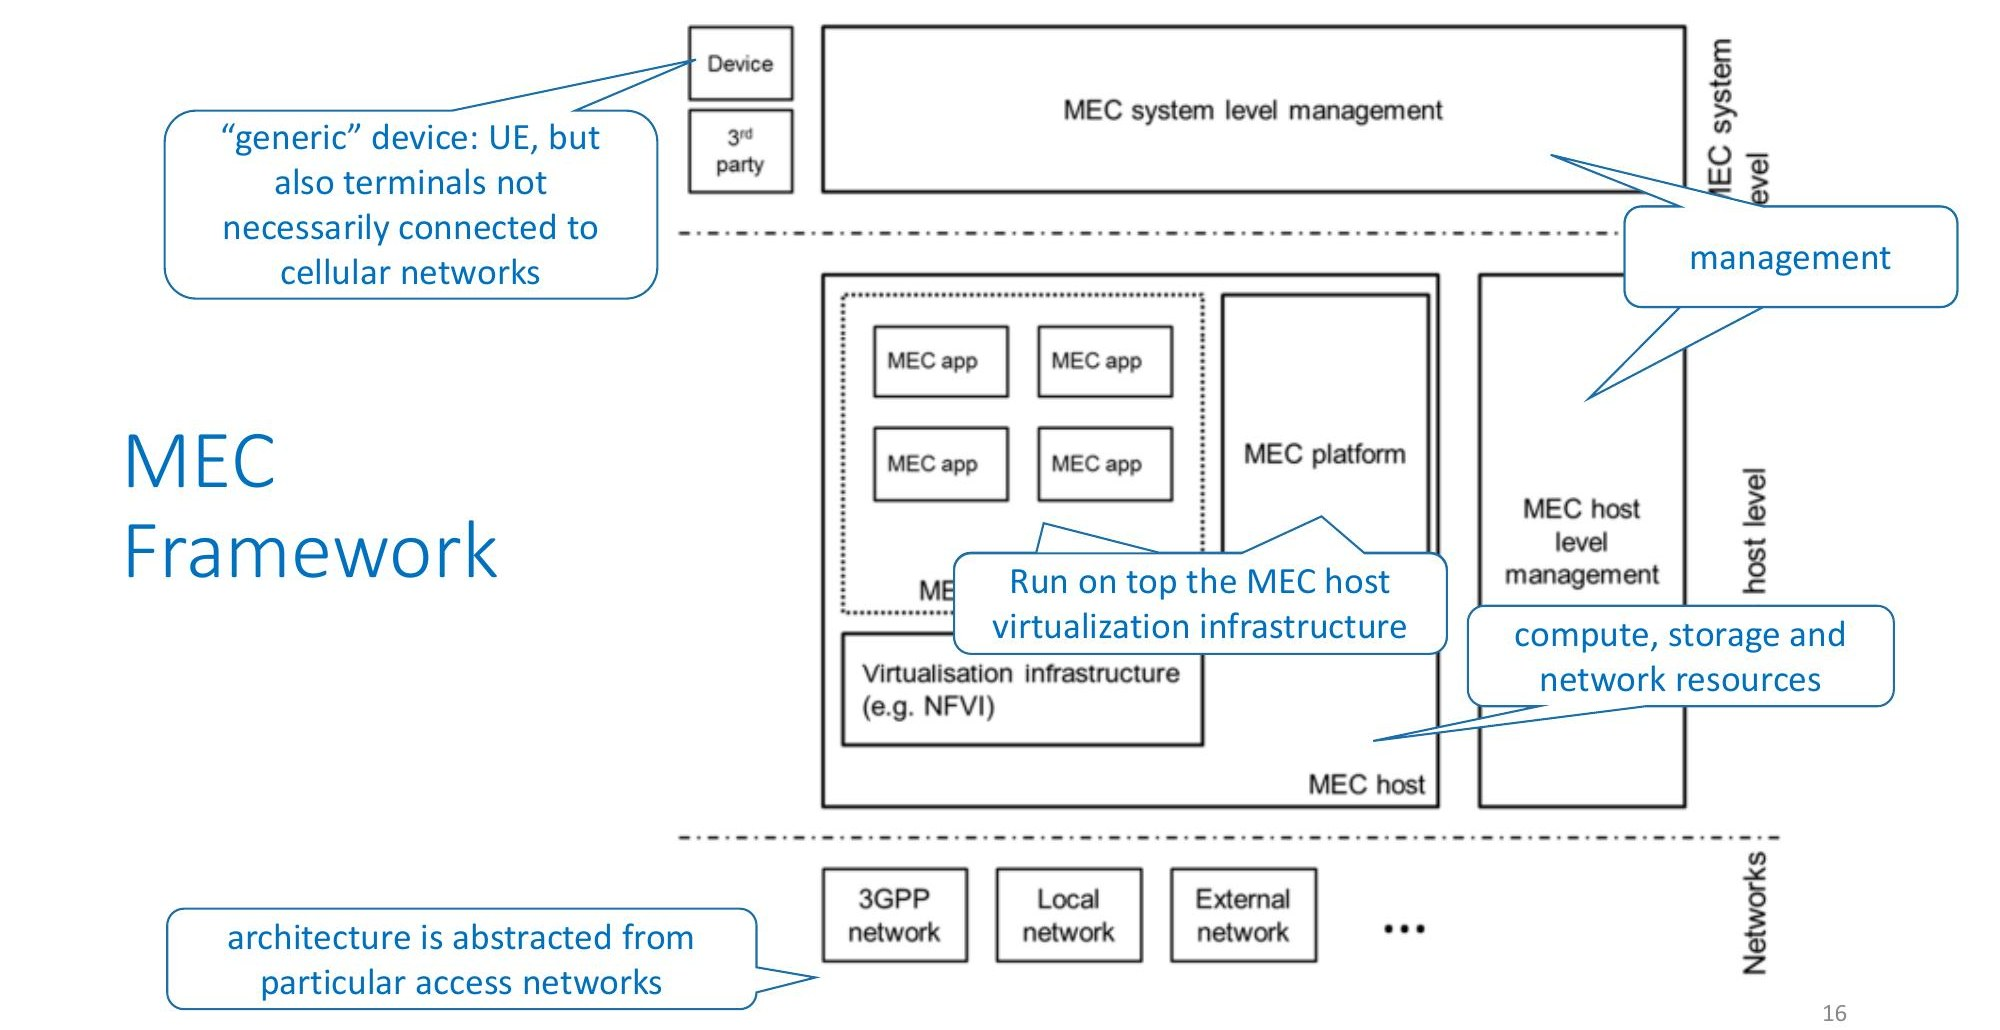
\includegraphics[keepaspectratio]{images/lezione-22-lab-multi-access-edge-computing-mec-img-06.jpg}}
\caption{17 --- Il MEC Framework ETSI.}
\end{figure}

\subsection{MEC API: Informazioni Locali e
Steering}\label{mec-api-informazioni-locali-e-steering}

Il MEC framework offre API per consumare servizi di rete in loco: -
\textbf{RNIS API}: Condizioni radio, Cell ID (per ottimizzazione
video/mobilità). - \textbf{Location API}: Geolocalizzazione e
Localizzazione logica. - \textbf{MTS (MultiAccess Traffic Steering)
API}: Gestisce il trade-off fondamentale tra \emph{Split traffic} (più
bandwidth unendo N link) e \emph{Duplicate traffic} (più affidabilità,
ridondando su N link per URLLC).

\begin{figure}
\centering
\pandocbounded{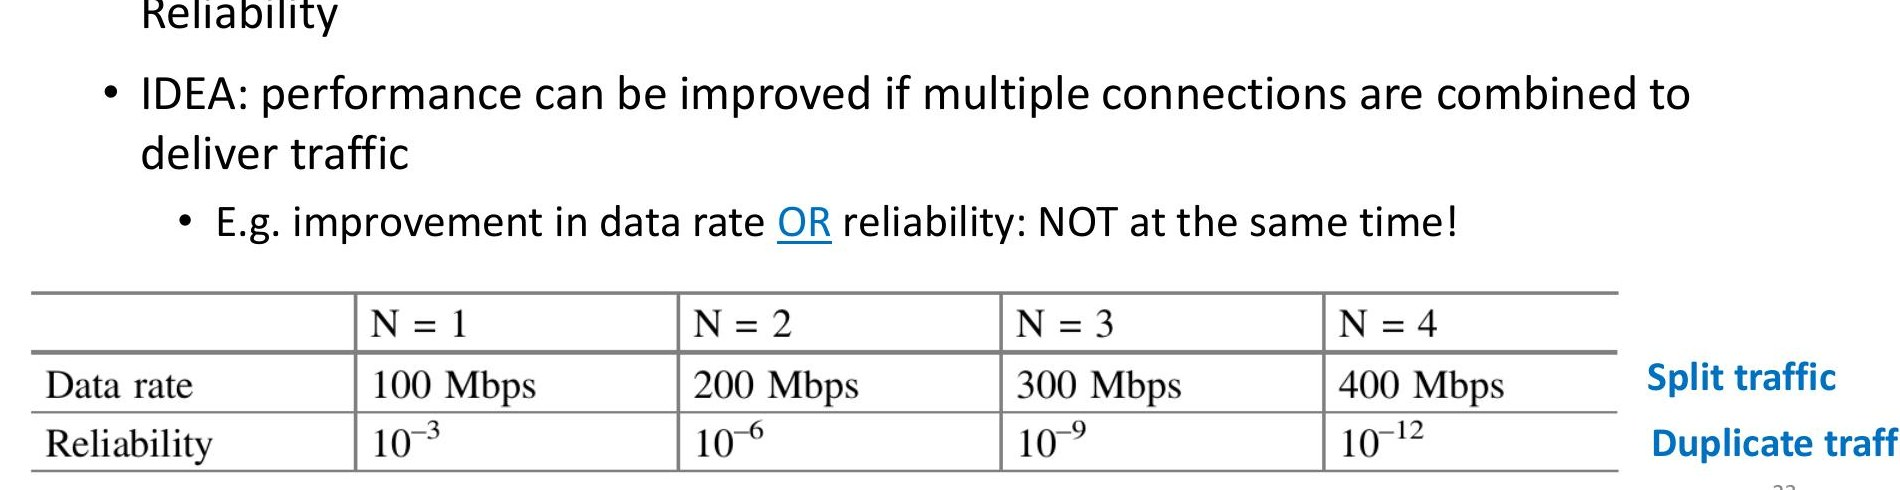
\includegraphics[keepaspectratio]{images/lezione-22-lab-multi-access-edge-computing-mec-img-07.jpg}}
\caption{18 --- Trade-off MTS tra Throughput (Split) e Affidabilità
(Duplicate).}
\end{figure}

\begin{center}\rule{0.5\linewidth}{0.5pt}\end{center}

\section{6. Network Slicing nel 5G ed Esercizio
Pratico}\label{network-slicing-nel-5g-ed-esercizio-pratico}

Il 5G accorpa requisiti antitetici: \textbf{mMTC} (massiva densità IoT),
\textbf{URLLC} (latenza ms e affidabilità estrema), \textbf{eMBB}
(altissima banda). La soluzione è il \textbf{Network Slicing}: creare
reti virtuali end-to-end con QoS garantita sulla stessa rete fisica. NFV
crea le funzioni, SDN gestisce l'isolamento dei flussi.

\begin{figure}
\centering
\pandocbounded{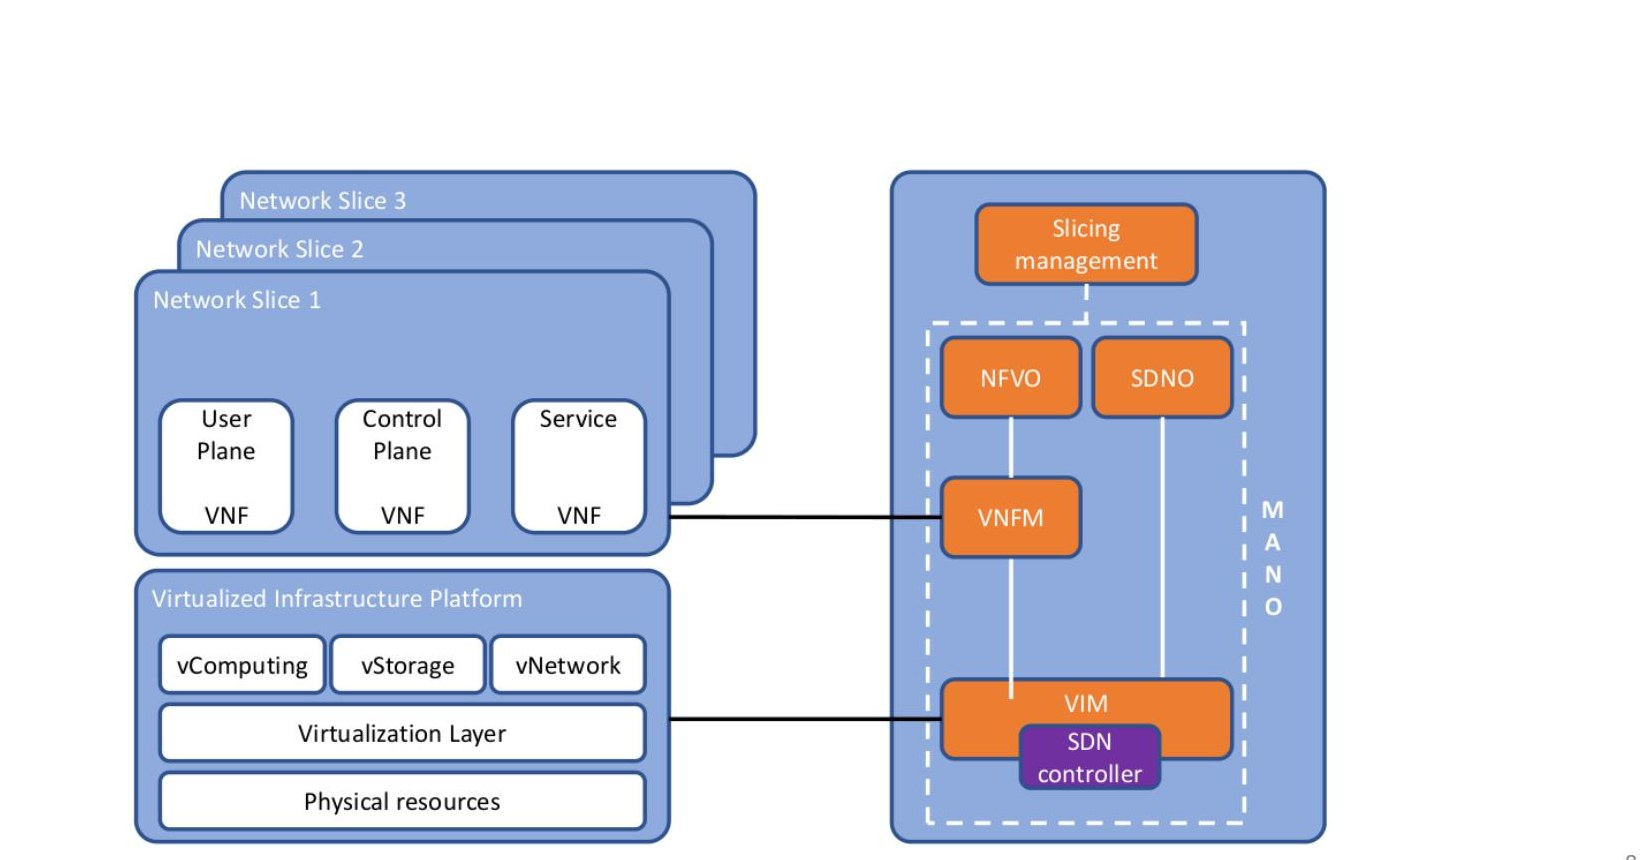
\includegraphics[keepaspectratio]{images/lezione-26-lab-network-slicing-img-01.jpg}}
\caption{19 --- Livelli architetturali per il slicing.}
\end{figure}

\subsection{Esperimento: Topology Slicing con
Ryu}\label{esperimento-topology-slicing-con-ryu}

Usando ComNetsEmu, realizziamo un anello di 4 switch (S1-S4) e
partizioniamo: - \textbf{Upper Slice}: h1 ↔ h3 su path a 10Mbps (via
S2). - \textbf{Lower Slice}: h2 ↔ h4 su path a 1Mbps (via S3).

\begin{figure}
\centering
\pandocbounded{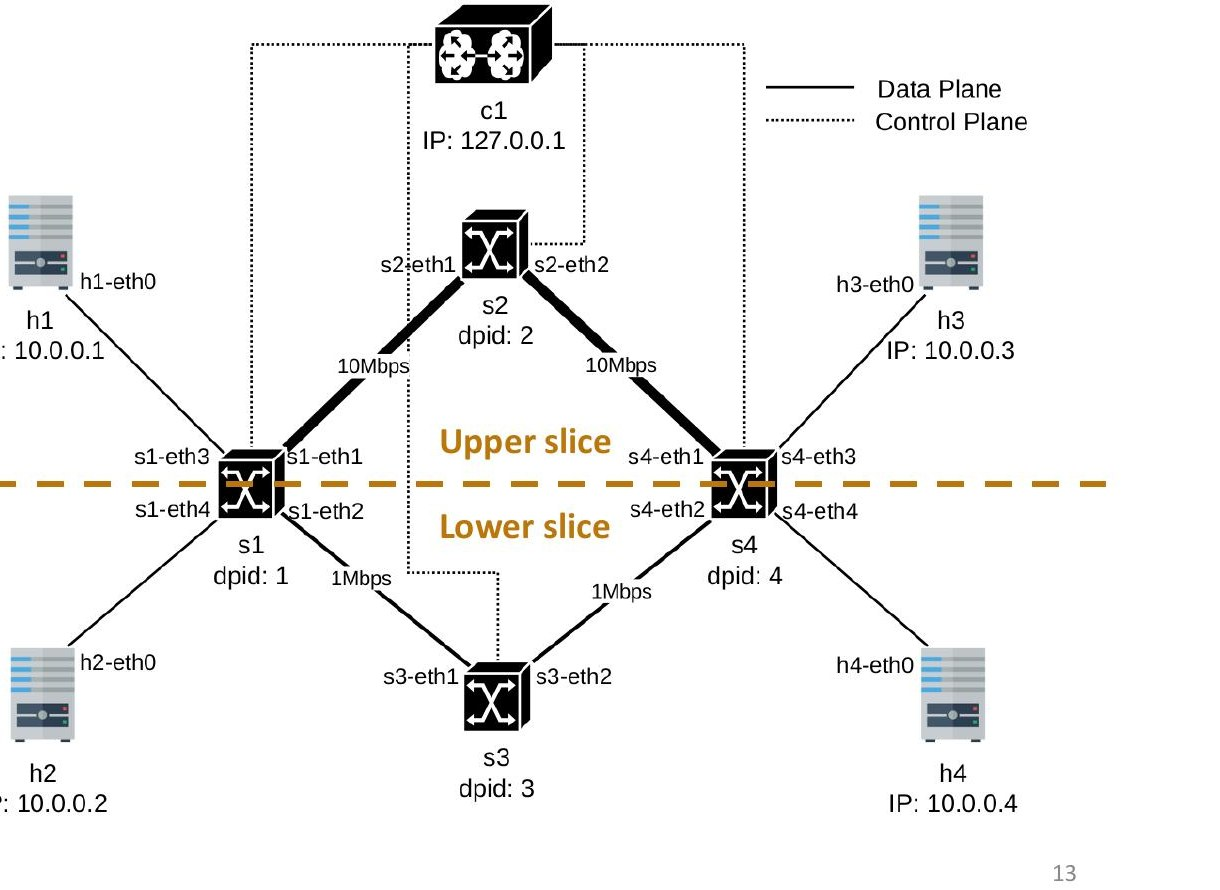
\includegraphics[keepaspectratio]{images/lezione-26-lab-network-slicing-img-03.jpg}}
\caption{20 --- Separazione Upper/Lower slice.}
\end{figure}

\textbf{Il Controller Ryu (\texttt{topologyslicing.py})}: Il
partizionamento avviene mappando staticamente le porte in
\texttt{slice\_to\_port} per gli switch di ingresso S1 e S4, garantendo
un rigido isolamento. Quando arriva il primo pacchetto
(\texttt{EventOFPPacketIn}), Ryu estrae \texttt{in\_port}, legge
\texttt{slice\_to\_port} e fissa la flow rule permanente sullo switch
con un \texttt{OFPFlowMod} via OpenFlow.

\begin{Shaded}
\begin{Highlighting}[]
\NormalTok{out\_port }\OperatorTok{=} \VariableTok{self}\NormalTok{.slice\_to\_port[dpid][in\_port]}
\NormalTok{actions }\OperatorTok{=}\NormalTok{ [datapath.ofproto\_parser.OFPActionOutput(out\_port)]}
\NormalTok{match }\OperatorTok{=}\NormalTok{ datapath.ofproto\_parser.OFPMatch(in\_port}\OperatorTok{=}\NormalTok{in\_port)}
\VariableTok{self}\NormalTok{.add\_flow(datapath, }\DecValTok{1}\NormalTok{, match, actions) }\CommentTok{\# Installa per i successivi}
\VariableTok{self}\NormalTok{.\_send\_package(msg, datapath, in\_port, actions) }\CommentTok{\# Inoltra l\textquotesingle{}attuale}
\end{Highlighting}
\end{Shaded}

\subsection{Esercizio B: Service Chain
Firewall}\label{esercizio-b-service-chain-firewall}

Inserendo manualmente uno switch S5 come Firewall tra S2-eth3 e S2-eth4:

\begin{Shaded}
\begin{Highlighting}[]
\ExtensionTok{**S2}\NormalTok{ redirige l}\StringTok{\textquotesingle{}Upper slice verso S5**}
\StringTok{mininet\textgreater{} sh ovs{-}ofctl add{-}flow s2 in\_port=1,priority=10,actions=output:3}
\StringTok{**S5 blocca il traffico ICMP tramite priorità OpenFlow**}
\StringTok{mininet\textgreater{} sh ovs{-}ofctl add{-}flow s5 icmp,priority=20,actions=drop}
\StringTok{mininet\textgreater{} sh ovs{-}ofctl add{-}flow s5 in\_port=1,priority=10,actions=output:2}
\end{Highlighting}
\end{Shaded}

Il traffico con match TCP/ICMP verrà bloccato prima dell'azione default
generica grazie alla \textbf{priority} maggiore.

\newpage

\chapter{05 - Preparazione Esame Orale}\label{preparazione-esame-orale}

Questo documento raccoglie le risposte complete a ciascuna delle
immagini del documento \emph{Questions for the oral exam 2023 --- Module
2}. Per ogni schema viene prima descritta l'immagine, poi illustrato
tutto ciò che va spiegato durante l'orale.

\begin{center}\rule{0.5\linewidth}{0.5pt}\end{center}

\section{Hidden Terminal (Terminale
Nascosto)}\label{hidden-terminal-terminale-nascosto}

\begin{figure}
\centering
\pandocbounded{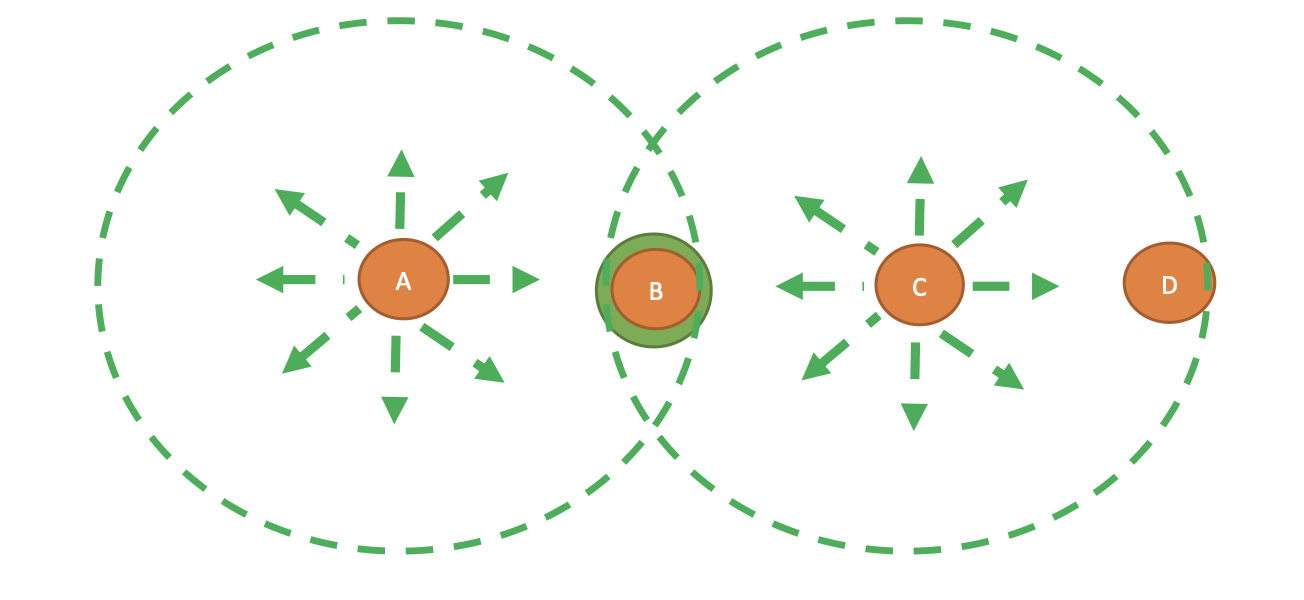
\includegraphics[keepaspectratio]{images/Pasted-image-20260429160400.png}}
\caption{\#\#\# Descrizione dell'immagine}
\end{figure}

Lo schema mostra quattro nodi etichettati A, B, C, D disposti in fila
orizzontale. Due cerchi tratteggiati di colore verde indicano i
rispettivi raggi di copertura radio: il primo include A e B (con
sovrapposizione al centro), il secondo include B e C. Il nodo D è fuori
dalla portata di entrambi. Il nodo B è evidenziato (cerchio verde più
spesso) perché è il ricevitore comune al centro della situazione.

\subsection{Cosa dire all'esame}\label{cosa-dire-allesame}

Il problema del \textbf{terminale nascosto} nasce da una limitazione
fisica fondamentale delle reti wireless: la potenza del segnale radio
cala con il quadrato della distanza, e la comunicazione può avvenire
solo tra nodi sufficientemente vicini. In questo scenario, A e C
vogliono entrambi trasmettere a B, ma A e C si trovano fuori dal raggio
radio l'uno dell'altro.

Supponiamo che A stia già trasmettendo verso B. La stazione C, prima di
trasmettere, esegue il \textbf{Carrier Sense}: ascolta il canale per
verificare se è libero. Poiché C non riesce a sentire il segnale di A
(sono fuori portata), C conclude erroneamente che il canale sia libero e
inizia a trasmettere verso B (o verso D). Il risultato è che i segnali
di A e di C si sovrappongono fisicamente nell'antenna di B, generando
una \textbf{collisione} che B riceve come segnale incomprensibile. Né A
né C rilevano la collisione, perché ciascuna sente solo il proprio
segnale (che è enormemente più forte di qualsiasi segnale di ritorno).

Questo è il motivo per cui il protocollo \textbf{CSMA/CD}, standard
nelle reti Ethernet cablate, non può essere usato nelle reti wireless:
il meccanismo di rilevamento delle collisioni richiede che il
trasmettitore possa ascoltare il canale mentre trasmette, il che è
impossibile in radio (il self-signal del trasmettitore è ordini di
grandezza più forte di qualsiasi segnale debole in arrivo).

\begin{callouttip}{Il punto chiave}

Con CSMA classico, il Carrier Sense viene eseguito dal trasmettitore, ma
quello che conta è lo stato del canale \textbf{al ricevitore}. Il
terminale nascosto è ``nascosto'' solo rispetto al trasmettitore
corrente, non rispetto al ricevitore.

\end{callouttip}

La soluzione a questo problema è il meccanismo \textbf{RTS/CTS},
descritto nel terzo schema.

\begin{center}\rule{0.5\linewidth}{0.5pt}\end{center}

\section{Exposed Terminal (Terminale
Esposto)}\label{exposed-terminal-terminale-esposto}

\pandocbounded{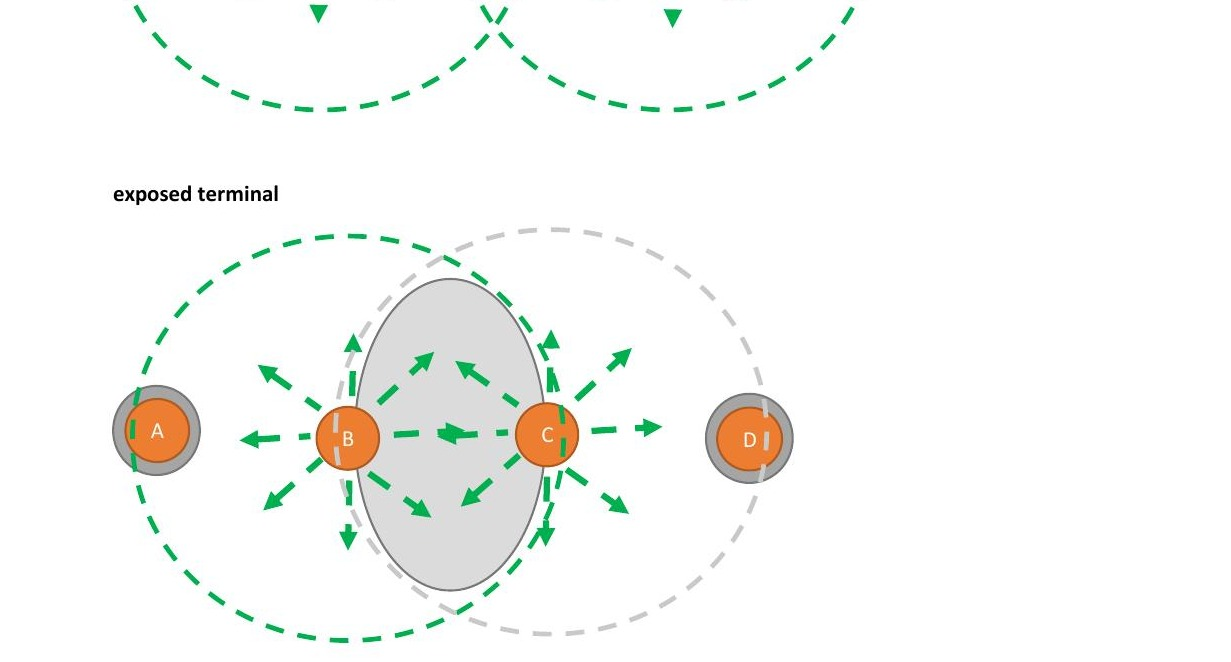
\includegraphics[keepaspectratio]{images/exam-mod2-exposed-terminal.jpg}}

\subsection{Descrizione dell'immagine}\label{descrizione-dellimmagine}

Lo schema mostra quattro nodi A, B, C, D in fila. A e D sono i nodi
periferici (grigi, fuori dal raggio di copertura della coppia centrale).
B e C si trovano al centro in sovrapposizione: il cerchio verde
tratteggiato principale copre B e C (e parte di A), mentre un cerchio
grigio parziale copre C e D. L'ellisse grigia al centro della figura
evidenzia la zona di interferenza comune tra B e C.

\subsection{Cosa dire all'esame}\label{cosa-dire-allesame-1}

Il problema del \textbf{terminale esposto} è speculare al precedente:
questa volta, una stazione si astiene inutilmente dal trasmettere perché
percepisce un segnale sul canale, anche se quel segnale non crea
interferenza al suo ricevitore di destinazione.

In questo scenario, B sta trasmettendo verso A. Il nodo C vuole inviare
un frame a D. Prima di trasmettere, C esegue il Carrier Sense e rileva
il segnale di B (che è vicino a C): applica la regola del CSMA e
conclude che il canale è occupato, rinviando la trasmissione. Ma questa
decisione è sbagliata: se C trasmettesse verso D, il segnale di C
raggiungerebbe D (che è fuori dalla portata di B), e le due
comunicazioni --- B→A e C→D --- potrebbero avvenire perfettamente in
parallelo senza interferirsi a vicenda.

C è chiamato \textbf{terminale esposto} alla trasmissione B→A:
``esposto'' nel senso che sente la trasmissione di B e ne è bloccato,
pur non essendo in conflitto reale con essa. Il risultato è un inutile
spreco di capacità: una comunicazione che potrebbe avvenire viene
soppressa per un falso allarme.

\begin{calloutwarning}{Attenzione}

Il terminale esposto non è un problema di collisione, ma di
\textbf{sotto-utilizzo del canale}. È meno grave del terminale nascosto
(che causa corruzioni di dati), ma riduce il throughput complessivo
della rete.

\end{calloutwarning}

Il meccanismo RTS/CTS del protocollo MACA risolve anche questo problema,
come illustrato nel terzo schema.

\begin{center}\rule{0.5\linewidth}{0.5pt}\end{center}

\section{RTS/CTS}\label{rtscts}

\pandocbounded{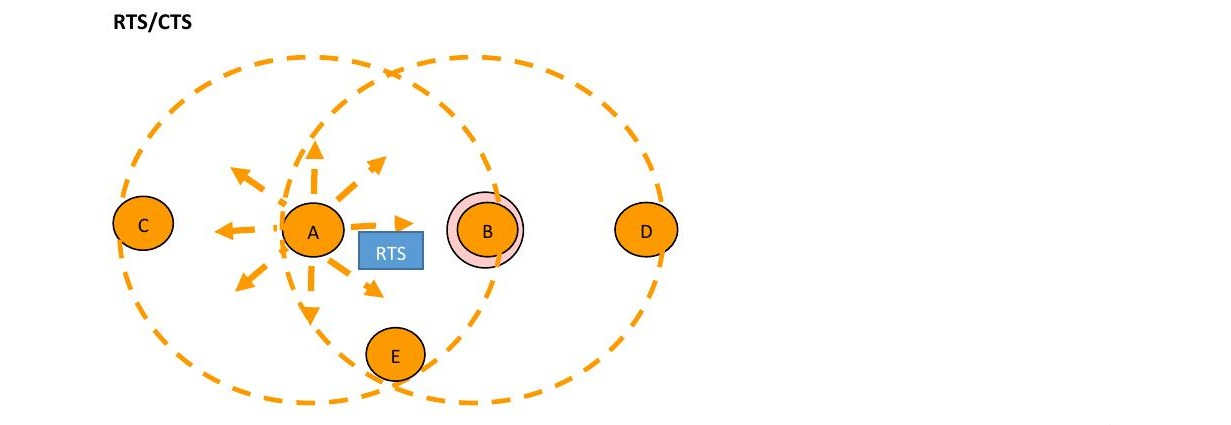
\includegraphics[keepaspectratio]{images/exam-mod2-rts-cts.jpg}}

\subsection{Descrizione dell'immagine}\label{descrizione-dellimmagine-1}

Lo schema mostra cinque nodi: C, A, B, D in fila orizzontale, e E sotto
la fila. Due grandi cerchi tratteggiati arancioni indicano i raggi di
copertura: il primo centrato su A copre C, A, B, E; il secondo centrato
su B copre A, B, D, E. La freccia arancione etichettata ``RTS'' va da A
verso B. I nodi B e A sono evidenziati con cerchi arancioni doppi (sono
gli attori principali). Il nodo E si trova nella sovrapposizione dei due
cerchi.

\subsection{Cosa dire all'esame}\label{cosa-dire-allesame-2}

Il meccanismo \textbf{RTS/CTS} (\emph{Request To Send / Clear To Send})
è il cuore del protocollo \textbf{MACA} (\emph{Multiple Access with
Collision Avoidance}, 1990) e del successivo \textbf{MACAW}, ed è
integrato nello standard \textbf{IEEE 802.11} (Wi-Fi). Risolve entrambi
i problemi del terminale nascosto e del terminale esposto prenotando il
canale in modo distribuito prima di trasmettere i dati.

Il funzionamento si articola in tre fasi:

\textbf{Fase 1 --- RTS}: quando A vuole inviare dati a B, invia prima un
breve pacchetto \textbf{RTS} (≈20 byte) che contiene: ID sorgente (A),
ID destinazione (B), e la \textbf{durata} del frame dati che seguirà.
Tutti i nodi nel raggio di A (ovvero C, B, E) ricevono questo RTS.

\textbf{Fase 2 --- CTS}: se B è libero e pronto, risponde con un
pacchetto \textbf{CTS} (anch'esso breve) che copia e ritrasmette la
durata dichiarata dall'RTS. Tutti i nodi nel raggio di B (ovvero A, D,
E) ricevono il CTS.

\textbf{Fase 3 --- DATA}: ricevuto il CTS, A inizia la trasmissione del
frame dati vero e proprio in condizioni sicure.

\textbf{Come risolve il terminale nascosto (D nel diagramma):} D non ha
sentito l'RTS di A (troppo lontano), ma riceve il CTS di B e capisce che
B è in procinto di ricevere dati. Quindi D si mette in silenzio per la
durata indicata nel CTS, evitando di interferire con la ricezione di B.

\textbf{Come risolve il terminale esposto (C nel diagramma):} C sente
l'RTS di A ma, essendo troppo lontano da B, non riceve il CTS di B. Da
questo C deduce di essere un terminale esposto: la comunicazione avviene
lontano dalla sua area di influenza, e può iniziare una propria
trasmissione senza creare interferenze.

\textbf{Il caso E:} E si trova nella zona di sovrapposizione, sente sia
l'RTS sia il CTS: sa con certezza di dover tacere per tutta la durata
della comunicazione.

\begin{callouttip}{Collisioni residue}

Con RTS/CTS le collisioni non scompaiono del tutto: possono ancora
avvenire tra pacchetti RTS (es. se C e D inviano contemporaneamente RTS
verso A). Ma in tal caso nessun dato applicativo viene perso, e lo
spreco di canale è minimo (RTS sono brevissimi). I mittenti applicano il
\textbf{Binary Exponential Backoff} prima di riprovare.

\end{callouttip}

In 802.11, l'impiego di RTS/CTS è configurabile tramite una soglia di
dimensione (\emph{RTS Threshold}): sempre, mai, o solo per frame sopra
una certa dimensione.

\begin{center}\rule{0.5\linewidth}{0.5pt}\end{center}

\section{Mobile Networks --- I}\label{mobile-networks-i}

\pandocbounded{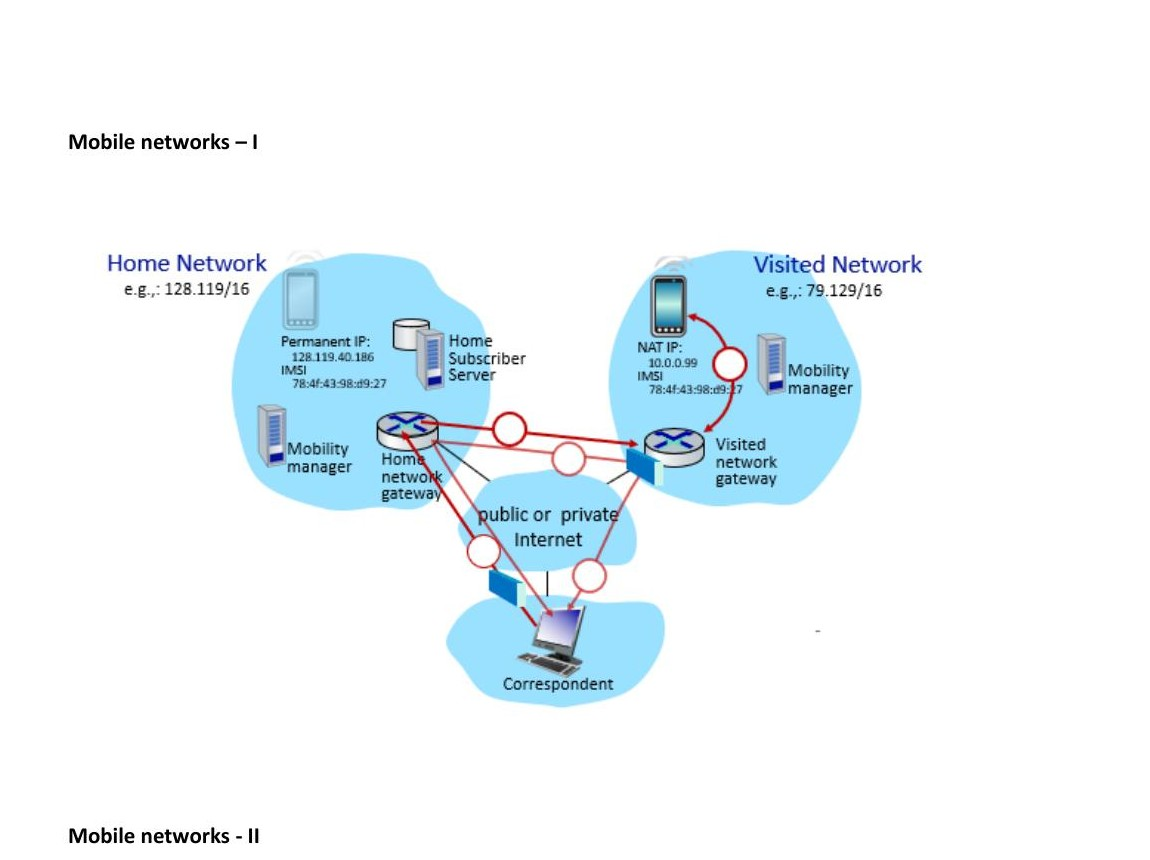
\includegraphics[keepaspectratio]{images/exam-mod2-mobile-networks-I.jpg}}

\subsection{Descrizione dell'immagine}\label{descrizione-dellimmagine-2}

Lo schema mostra un'architettura a tre attori principali. A sinistra, la
\textbf{Home Network} (sfondo azzurro) con: un dispositivo mobile
(smartphone), il Permanent IP 128.119.40.186, IMSI 78:4f:43:98:d9:27, il
Home Subscriber Server, il Mobility Manager, e il Home network gateway.
A destra, la \textbf{Visited Network} (sfondo azzurro) con: lo
smartphone mobile (con NAT IP 10.0.0.99, stesso IMSI), il Mobility
Manager, e il Visited network gateway. Al centro in basso c'è il
\textbf{Correspondent} (laptop) connesso attraverso il public/private
Internet. Le frecce mostrano connessioni tra Home gateway, Visited
gateway e Correspondent, formando un triangolo di routing.

\subsection{Cosa dire all'esame}\label{cosa-dire-allesame-3}

Questo schema illustra l'architettura del \textbf{routing indiretto}
(\emph{triangle routing}) nelle reti mobili 4G/5G, che è il meccanismo
standard usato nelle reti LTE.

L'idea di base è che ogni utente mobile abbia una \textbf{home network}:
la rete dell'operatore con cui ha sottoscritto il contratto (es.
Verizon, TIM). Questa rete mantiene un database centralizzato,
l'\textbf{Home Subscriber Server (HSS)}, che registra l'identità
dell'utente (IMSI) e i servizi abilitati. Quando il dispositivo lascia
la home network ed entra in una \textbf{visited network} (roaming),
mantiene il suo indirizzo IP permanente (128.119.40.186) ma ottiene
temporaneamente un indirizzo locale nella rete visitata (NAT IP:
10.0.0.99).

La \textbf{fase di registrazione} avviene così: il dispositivo si
associa alla BS della rete visitata e si identifica tramite IMSI → il
Mobility Manager della rete visitata contatta l'HSS della home network →
l'HSS aggiorna la posizione del dispositivo e restituisce i parametri di
autenticazione → da questo momento l'HSS sa dove si trova il
dispositivo.

Nel \textbf{routing indiretto}, quando il Correspondent vuole inviare
dati al dispositivo mobile: 1. Il Correspondent invia il pacchetto
all'\textbf{indirizzo permanente} del mobile (128.119.40.186), che
appartiene alla home network. 2. Il \textbf{Home network gateway} riceve
il pacchetto, lo \textbf{incapsula} in un tunnel (tipicamente usando il
protocollo GTP --- \emph{GPRS Tunneling Protocol}) e lo forwarda al
Visited network gateway. 3. Il \textbf{Visited network gateway}
decapsula il pacchetto, applica la traduzione \textbf{NAT} (perché il
dispositivo ha un IP locale 10.0.0.99) e lo consegna al dispositivo. 4.
Le risposte del dispositivo possono seguire il percorso inverso oppure
essere inviate direttamente al Correspondent.

Il percorso forma un \textbf{triangolo}: Correspondent → Home → Visited
→ Mobile, anche se Correspondent e mobile fossero fisicamente vicini.
Questo è il costo dell'approccio, ma il beneficio è che ogni cambio di
rete visitata è \textbf{trasparente} per il Correspondent: la home
network aggiorna silenziosamente l'endpoint del tunnel, senza che il
Correspondent debba fare nulla.

\begin{center}\rule{0.5\linewidth}{0.5pt}\end{center}

\section{Mobile Networks --- II}\label{mobile-networks-ii}

\pandocbounded{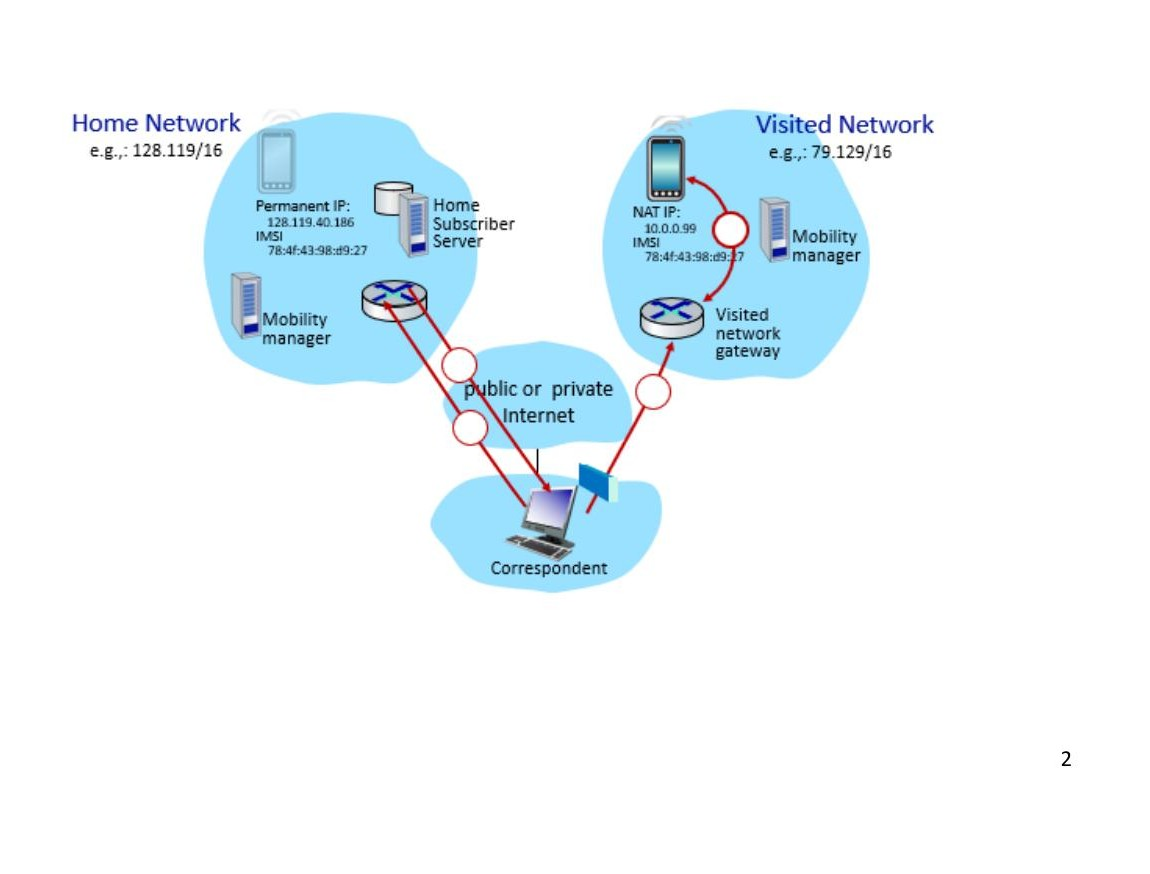
\includegraphics[keepaspectratio]{images/exam-mod2-mobile-networks-II.jpg}}

\subsection{Descrizione dell'immagine}\label{descrizione-dellimmagine-3}

Lo schema mostra la stessa architettura del precedente (Home Network con
HSS, Mobility Manager, Home gateway; Visited Network con Mobility
Manager, Visited gateway; Correspondent in basso), ma con un percorso di
frecce diverso: il Correspondent sembra comunicare direttamente con il
Visited network gateway, senza passare per il Home gateway.

\subsection{Cosa dire all'esame}\label{cosa-dire-allesame-4}

Questo schema illustra il \textbf{routing diretto}, l'alternativa al
triangle routing per le reti mobili.

Nel routing diretto, il Correspondent non invia i pacchetti
all'indirizzo permanente del mobile, ma ottiene prima il suo
\textbf{care-of address} nella rete visitata. La procedura è la
seguente:

\begin{enumerate}
\def\labelenumi{\arabic{enumi}.}
\tightlist
\item
  Il Correspondent interroga l'\textbf{HSS} della home network (tramite
  un protocollo apposito) per ottenere l'indirizzo corrente del
  dispositivo mobile nella rete visitata (il care-of address, es.
  10.0.0.99).
\item
  Il Correspondent invia i pacchetti \textbf{direttamente} al care-of
  address nella visited network, bypassando la home network.
\item
  Il Visited network gateway riceve il pacchetto e lo consegna al
  dispositivo mobile.
\end{enumerate}

\textbf{Vantaggi rispetto al routing indiretto:} il percorso è più corto
(nessun triangolo), la latenza è ridotta, e non si sovraccarica
inutilmente la home network.

\textbf{Svantaggi e problemi:} l'approccio \textbf{non è trasparente}
per il Correspondent, che deve eseguire attivamente la query all'HSS.
Inoltre, se il dispositivo cambia rete visitata durante una sessione
attiva, il Correspondent ha interrogato l'HSS solo all'inizio della
sessione e non conosce il nuovo care-of address: servono meccanismi
aggiuntivi (es. forwarding dalla vecchia visited network alla nuova, o
re-query dell'HSS). Nel routing indiretto, invece, è sufficiente
aggiornare l'endpoint del tunnel lato home network.

\begin{callouttip}{Confronto diretto vs indiretto}

{\def\LTcaptype{none} % do not increment counter
\begin{longtable}[]{@{}
  >{\raggedright\arraybackslash}p{(\linewidth - 4\tabcolsep) * \real{0.3333}}
  >{\raggedright\arraybackslash}p{(\linewidth - 4\tabcolsep) * \real{0.3333}}
  >{\raggedright\arraybackslash}p{(\linewidth - 4\tabcolsep) * \real{0.3333}}@{}}
\toprule\noalign{}
\begin{minipage}[b]{\linewidth}\raggedright
Aspetto
\end{minipage} & \begin{minipage}[b]{\linewidth}\raggedright
Routing Indiretto
\end{minipage} & \begin{minipage}[b]{\linewidth}\raggedright
Routing Diretto
\end{minipage} \\
\midrule\noalign{}
\endhead
\bottomrule\noalign{}
\endlastfoot
Percorso pacchetti & Triangolo (via home) & Diretto alla visited \\
Trasparenza per Correspondent & Sì & No (deve interrogare HSS) \\
Gestione cambio rete & Automatica (re-tunnel) & Complessa (deve
aggiornare il Correspondent) \\
Latenza & Maggiore (percorso più lungo) & Minore \\
Adottato in LTE/4G & Sì (per default) & Solo con ottimizzazione
esplicita \\
\end{longtable}
}

\end{callouttip}

\begin{center}\rule{0.5\linewidth}{0.5pt}\end{center}

\section{Mobile Networks --- III}\label{mobile-networks-iii}

\pandocbounded{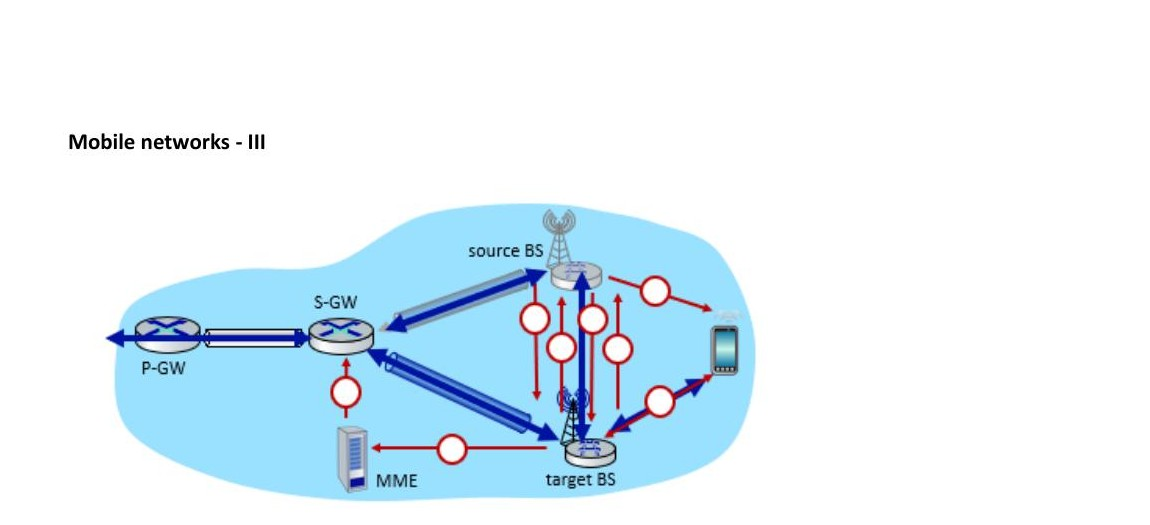
\includegraphics[keepaspectratio]{images/exam-mod2-mobile-networks-III.jpg}}

\subsection{Descrizione dell'immagine}\label{descrizione-dellimmagine-4}

Lo schema mostra l'architettura di una rete LTE durante un
\textbf{handover} tra celle. Sono visibili: in alto a destra la
\textbf{source BS} (Base Station sorgente, la torre radio da cui il
dispositivo si sta spostando), in basso a destra la \textbf{target BS}
(Base Station di destinazione, quella verso cui il dispositivo si sta
muovendo). Al centro c'è l'\textbf{S-GW} (\emph{Serving Gateway}), a
sinistra il \textbf{P-GW} (\emph{PDN Gateway}), e in basso al centro il
\textbf{MME} (\emph{Mobility Management Entity}). Le frecce indicano i
percorsi di segnalazione e dati durante l'handover.

\subsection{Cosa dire all'esame}\label{cosa-dire-allesame-5}

Questo schema mostra la procedura di \textbf{handover tra Base Station}
in una rete 4G LTE, ovvero il meccanismo che consente a un dispositivo
in movimento di passare da una cella all'altra senza perdere la
connessione.

\textbf{Architettura del piano dati:} quando il dispositivo è associato
a una BS, il traffico dati fluisce attraverso due tunnel GTP in cascata:
- \textbf{Tunnel BS ↔ S-GW}: connette la Base Station corrente al
Serving Gateway. - \textbf{Tunnel S-GW ↔ P-GW}: connette il Serving
Gateway al PDN Gateway (il gateway verso Internet nella home network),
realizzando il routing indiretto.

\textbf{Procedura di handover (7 passi):}

\begin{enumerate}
\def\labelenumi{\arabic{enumi}.}
\tightlist
\item
  La \textbf{source BS} rileva il degrado del segnale (o il
  sovraccarico) e decide di avviare l'handover. Sceglie la
  \textbf{target BS} (sulla base delle misure di segnale riportate dal
  dispositivo) e le invia una \textbf{Handover Request}.
\item
  La \textbf{target BS} pre-alloca le risorse radio necessarie e
  risponde con un \textbf{Handover Request ACK} contenente i parametri
  di configurazione per il dispositivo.
\item
  La \textbf{source BS} notifica al dispositivo il cambio imminente; da
  questo momento il dispositivo può già trasmettere tramite la nuova BS
  --- dal punto di vista del dispositivo l'handover è già avvenuto.
\item
  La \textbf{source BS} smette di trasmettere al dispositivo e inizia a
  \textbf{forwardare} i datagrammi in arrivo verso la target BS (che li
  recapita al dispositivo via radio).
\item
  La \textbf{target BS} informa l'\textbf{MME} di essere la nuova BS per
  il dispositivo.
\item
  L'\textbf{MME} istruisce lo \textbf{S-GW} di aggiornare l'endpoint del
  tunnel dati alla nuova target BS. La source BS riceve conferma e
  libera le risorse radio.
\item
  Il traffico fluisce ora attraverso il \textbf{nuovo tunnel} target BS
  ↔ S-GW, mentre il tunnel S-GW ↔ P-GW rimane invariato.
\end{enumerate}

\begin{callouttip}{Chi decide l’handover?}

È un punto classico da esame: la \textbf{source BS} decide sia di
avviare l'handover sia di scegliere la target BS --- non l'MME. L'MME
viene coinvolto solo nella fase finale per aggiornare il piano dati.
Questo riflette la separazione tra control plane (MME gestisce la
mobilità a livello di rete) e data plane (le BS gestiscono la qualità
del segnale radio).

\end{callouttip}

\begin{calloutnote}{Continuità delle sessioni TCP}

Durante l'handover possono andare persi alcuni datagrammi in transito.
Tuttavia le sessioni TCP rimangono attive: dal punto di vista del
Correspondent, la posizione del mobile è un dettaglio interno alla home
network gestito trasparentemente dal meccanismo di tunneling.

\end{calloutnote}

\begin{center}\rule{0.5\linewidth}{0.5pt}\end{center}

\section{SDN --- Generalized
Forwarding}\label{sdn-generalized-forwarding}

\pandocbounded{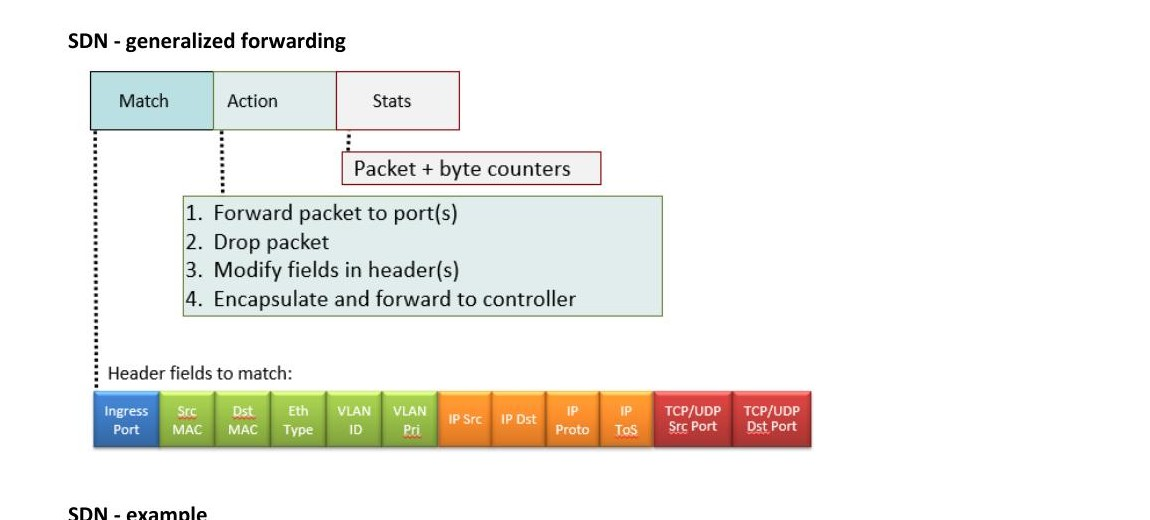
\includegraphics[keepaspectratio]{images/exam-mod2-sdn-generalized-forwarding.jpg}}

\subsection{Descrizione dell'immagine}\label{descrizione-dellimmagine-5}

Lo schema mostra la struttura di una \textbf{flow table entry} OpenFlow
con tre colonne: \textbf{Match} (a sinistra, punteggiata),
\textbf{Action} (al centro, che elenca 4 azioni possibili),
\textbf{Stats} (a destra, che mostra ``Packet + byte counters''). Nella
sezione Action si legge: 1. Forward packet to port(s), 2. Drop packet,
3. Modify fields in header(s), 4. Encapsulate and forward to controller.
Nella parte inferiore, una riga mostra i campi dell'header su cui si fa
il match: Ingress Port, Src MAC, Dst MAC, Eth Type, VLAN ID, VLAN Pri,
IP Src, IP Dst, IP Proto, IP ToS, TCP/UDP Src Port, TCP/UDP Dst Port.

\subsection{Cosa dire all'esame}\label{cosa-dire-allesame-6}

Questo schema illustra il concetto di \textbf{forwarding generalizzato}
(\emph{generalized forwarding}) in SDN, che è l'astrazione fondamentale
che rende il data plane programmabile.

Nell'approccio tradizionale, i router inoltrano i pacchetti basandosi
\textbf{solo sull'indirizzo IP di destinazione} (\emph{destination-based
forwarding}). OpenFlow generalizza questo concetto con l'astrazione
\textbf{match-action}: ogni pacchetto viene confrontato con le regole
nella flow table, e quando c'è un match, viene eseguita l'azione
corrispondente.

\textbf{I campi di match} possono essere qualsiasi combinazione dei
seguenti: - Livello 1: \textbf{Ingress Port} (la porta fisica da cui è
arrivato il pacchetto) - Livello 2 (Datalink): Src MAC, Dst MAC, Eth
Type, VLAN ID, VLAN Priority - Livello 3 (Rete): IP Src, IP Dst, IP
Protocol, IP ToS - Livello 4 (Trasporto): TCP/UDP Src Port, TCP/UDP Dst
Port

Questo consente di distinguere flussi in base a qualsiasi combinazione
di questi campi: non solo la destinazione IP, ma anche il protocollo, le
porte, le VLAN, ecc. Si parla di \textbf{flow-based forwarding}.

\textbf{Le azioni possibili} sono: 1. \textbf{Forward to port(s)}: invia
il pacchetto su una o più porte (forwarding normale, broadcast,
multicast). 2. \textbf{Drop}: scarta il pacchetto (firewall, access
control). 3. \textbf{Modify fields in header}: modifica campi
dell'intestazione prima di forwardare (NAT, QoS marking, VLAN tagging).
4. \textbf{Encapsulate and forward to controller}: invia il pacchetto al
controller SDN per una decisione centralizzata (usato per pacchetti non
matchati da nessuna regola --- \emph{table-miss}).

\textbf{Stats}: ogni entry mantiene contatori di pacchetti e byte, utili
per monitoring e traffic engineering.

\begin{callouttip}{Generalità del match-action}

L'astrazione match-action è sufficientemente generale da esprimere:
routing IP (match su IP dst), load balancing (match su src/dst + hash),
firewall (match su src/dst/protocol + drop), NAT (match + modify). Un
singolo modello unifica dispositivi che nelle reti tradizionali
richiederebbero apparati separati.

\end{callouttip}

\begin{center}\rule{0.5\linewidth}{0.5pt}\end{center}

\section{SDN --- Example}\label{sdn-example}

\pandocbounded{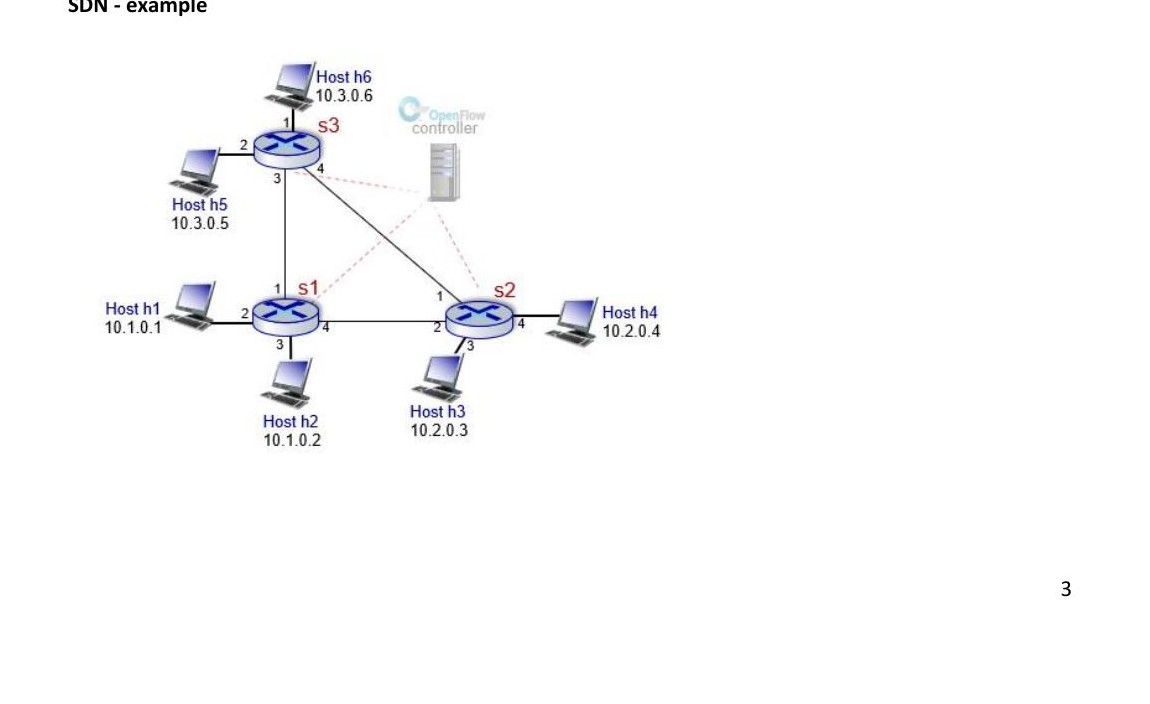
\includegraphics[keepaspectratio]{images/exam-mod2-sdn-example.jpg}}

\subsection{Descrizione dell'immagine}\label{descrizione-dellimmagine-6}

Lo schema mostra una topologia di rete con tre switch SDN (s1, s2, s3) e
sei host: h1 (10.1.0.1), h2 (10.1.0.2), h3 (10.2.0.3), h4 (10.2.0.4), h5
(10.3.0.5), h6 (10.3.0.6). S1 è connesso a h1, h2, s2 e s3. S2 è
connesso a s1, h3, h4. S3 è connesso a s1, h5, h6. Un \textbf{OpenFlow
controller} è connesso a s3 (e tramite essa all'intera rete). Ogni porta
degli switch è numerata.

\subsection{Cosa dire all'esame}\label{cosa-dire-allesame-7}

Questo schema è un esempio concreto di rete gestita con SDN per mostrare
come il \textbf{control plane centralizzato} possa implementare
politiche impossibili con il routing tradizionale.

Nell'architettura mostrata, il \textbf{controller OpenFlow} mantiene una
visione globale della topologia: conosce tutti gli switch, tutte le loro
porte, e dove si trovano i vari host. Le flow table degli switch s1, s2,
s3 vengono popolate \textbf{dal controller}, non calcolate localmente
dagli switch.

\textbf{Traffic Engineering con SDN:} supponiamo che il controller
voglia bilanciare il traffico da h1 (10.1.0.1) verso h4 (10.2.0.4) su
due percorsi: - Percorso A: h1 → s1 → s2 → h4 - Percorso B: h1 → s1 → s3
→ s2 → h4

Con il routing IP tradizionale questo è impossibile: l'algoritmo SPF
converge su un solo percorso minimo. Con SDN, il controller installa
regole diverse in s1 per flussi diversi (es. dividendo per porta
sorgente TCP), realizzando il load balancing.

\textbf{Forwarding basato su flusso:} il controller può distinguere il
traffico h1→h4 dal traffico h2→h4 e applicare politiche diverse. Ad
esempio: - Traffico h1→h4: percorso s1→s2, priorità alta - Traffico
h2→h4: percorso s1→s3→s2, priorità normale

Questo è il \textbf{routing per-flusso}, impossibile nel routing
tradizionale destination-based.

\textbf{Topology discovery:} il controller scopre la topologia inviando
pacchetti LLDP (\emph{Link Layer Discovery Protocol}) tramite gli
switch. Ogni switch incapsula un pacchetto LLDP e lo invia su tutte le
porte; quando un altro switch lo riceve, lo invia al controller, che
così ricostruisce le connessioni tra switch.

\begin{center}\rule{0.5\linewidth}{0.5pt}\end{center}

\section{SDN --- Architecture}\label{sdn-architecture}

\pandocbounded{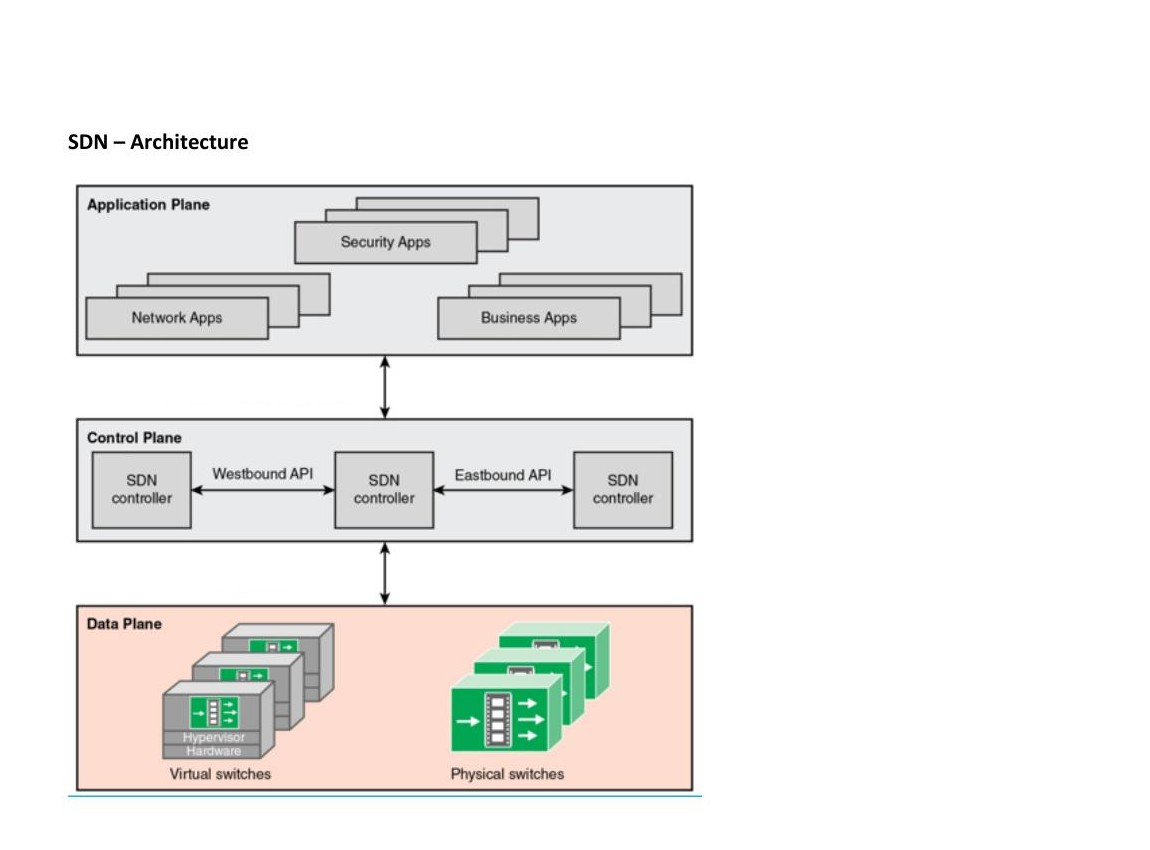
\includegraphics[keepaspectratio]{images/exam-mod2-sdn-architecture.jpg}}

\subsection{Descrizione dell'immagine}\label{descrizione-dellimmagine-7}

Lo schema mostra l'architettura SDN a tre livelli sovrapposti. Il
livello superiore è l'\textbf{Application Plane} con tre categorie di
applicazioni: Network Apps, Security Apps, Business Apps. Il livello
centrale è il \textbf{Control Plane} con tre SDN controller connessi
orizzontalmente tramite \textbf{Westbound API} e \textbf{Eastbound API}.
Il livello inferiore è il \textbf{Data Plane} con virtual switches (a
sinistra, su hypervisor/hardware) e physical switches (a destra). Tra
Application Plane e Control Plane c'è una freccia bidirezionale
(Northbound API); tra Control Plane e Data Plane c'è un'altra freccia
bidirezionale (Southbound API).

\subsection{Cosa dire all'esame}\label{cosa-dire-allesame-8}

Questo schema illustra l'\textbf{architettura a tre livelli di SDN}, che
realizza la separazione netta tra data plane, control plane e
application plane.

\textbf{Data Plane (Livello inferiore):} contiene gli switch del data
plane, che possono essere sia fisici (hardware commodity a basso costo)
sia virtuali (Open vSwitch su hypervisor). Sono dispositivi semplici: il
loro unico compito è applicare meccanicamente le regole di forwarding
(match-action) ai pacchetti in transito secondo le flow table installate
dal controller. Non calcolano nulla autonomamente.

\textbf{Control Plane (Livello centrale):} contiene il controller SDN, o
meglio una \textbf{rete di controller SDN} distribuiti. Sebbene appaia
come un'entità logicamente centralizzata (ha una visione globale della
rete), è implementato fisicamente come sistema distribuito per garantire
tolleranza ai guasti e scalabilità. Il controller mantiene: la topologia
della rete, le statistiche dei flussi, i link attivi, le tabelle di
forwarding. Comunica verso il basso con il Data Plane tramite la
\textbf{Southbound API} (tipicamente OpenFlow), e verso l'alto con le
applicazioni tramite la \textbf{Northbound API}. I controller comunicano
tra loro tramite \textbf{Westbound/Eastbound API} per sincronizzare lo
stato globale.

\textbf{Application Plane (Livello superiore):} contiene le applicazioni
di controllo della rete (\emph{network-control applications}), il vero
``cervello'' del sistema. Sono \textbf{unbundled}: possono essere
sviluppate da terze parti indipendentemente dai produttori hardware e
software del controller. Esempi: load balancer, firewall, traffic
engineering, monitoraggio, rilevamento anomalie. Le applicazioni
esprimono policy di alto livello al controller tramite la Northbound
API.

\begin{calloutnote}{Il valore dell’architettura a livelli}

La separazione in tre piani replica il principio dei livelli di
astrazione di Internet. Ogni livello si può evolvere indipendentemente:
nuovi algoritmi di routing nel Control Plane, nuove applicazioni
nell'Application Plane, nuovo hardware nel Data Plane --- senza impatto
sugli altri livelli. Questo è il vantaggio principale rispetto alle reti
tradizionali con logica chiusa nell'hardware proprietario.

\end{calloutnote}

\begin{center}\rule{0.5\linewidth}{0.5pt}\end{center}

\section{OpenFlow Switch}\label{openflow-switch-1}

\pandocbounded{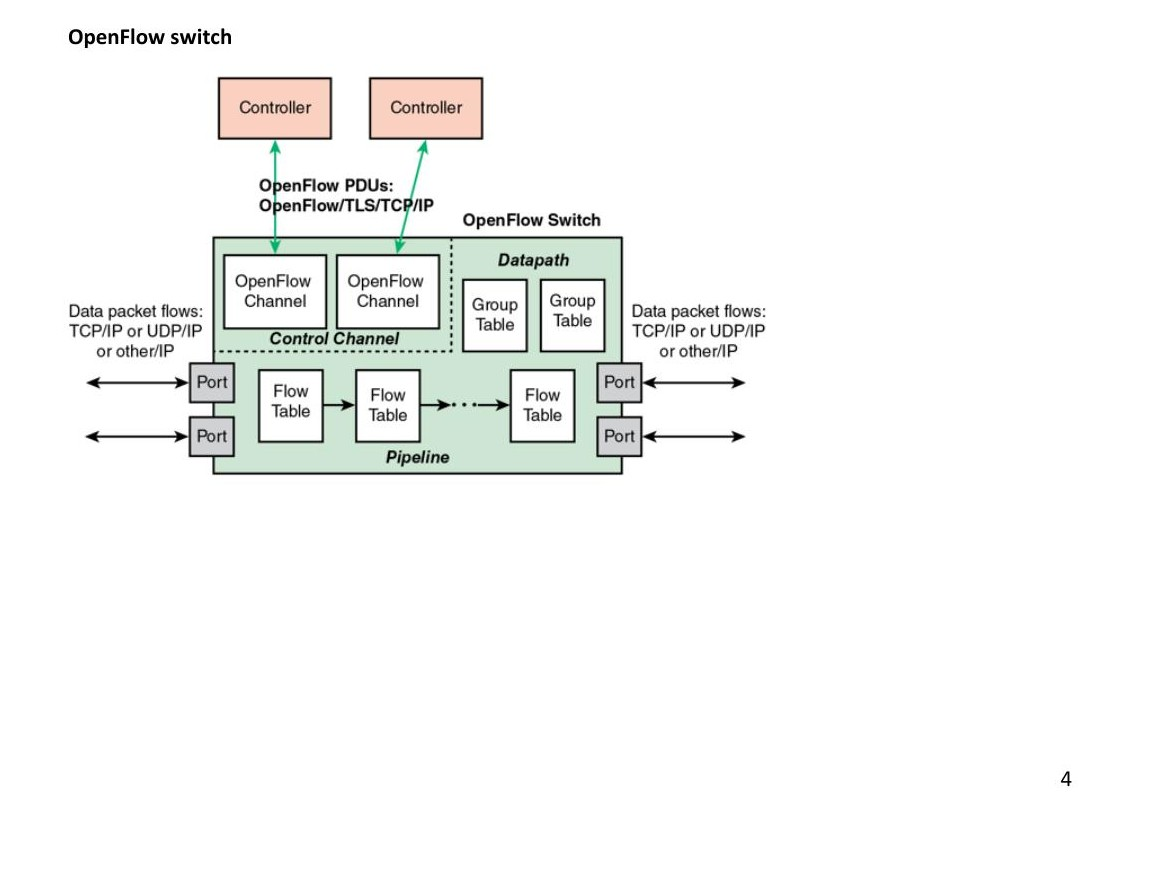
\includegraphics[keepaspectratio]{images/exam-mod2-openflow-switch.jpg}}

\subsection{Descrizione dell'immagine}\label{descrizione-dellimmagine-8}

Lo schema mostra l'architettura interna di un \textbf{OpenFlow Switch}.
A sinistra e a destra ci sono i \textbf{Data packet flows} (TCP/IP o
UDP/IP). All'interno dello switch sono evidenziate due aree: il
\textbf{Datapath} (in alto, che contiene Group Tables) e il
\textbf{Pipeline} (in basso, che contiene una catena di Flow Tables). Il
\textbf{Control Channel} (area centrale) ospita due \textbf{OpenFlow
Channels} connessi ai rispettivi Controller (in alto). Le porte (Port)
connettono l'esterno al pipeline interno.

\subsection{Cosa dire all'esame}\label{cosa-dire-allesame-9}

Lo schema illustra l'architettura interna di uno switch OpenFlow,
distinguendo il \textbf{piano dati interno} (\emph{Datapath}) dal
\textbf{canale di controllo} (\emph{Control Channel}).

\textbf{Ports:} lo switch ha porte fisiche su cui arrivano e partono i
data packet flow (TCP/IP, UDP/IP, altri). Sono le interfacce verso la
rete esterna.

\textbf{Pipeline di Flow Table:} quando un pacchetto entra in una porta,
viene processato attraverso una catena (\emph{pipeline}) di Flow Table
in sequenza, dalla tabella 0 in poi. In ogni tabella si cerca un match
con le regole installate dal controller: - Se c'è un match → si esegue
l'azione (forward, drop, modify, ecc.) e si passa alla tabella
successiva o si finalizza. - Se non c'è match → si applica la regola di
\emph{table-miss} (tipicamente: invia al controller per una decisione).

\textbf{Group Tables:} le Group Tables consentono azioni più complesse
che non si possono esprimere con le semplici Flow Table: ad esempio la
replica di un pacchetto su più porte (multicast/broadcast), il
fast-failover (selezionare automaticamente una porta alternativa se
quella principale è down), o il load balancing su un gruppo di porte.

\textbf{Control Channel:} è il canale sicuro (tipicamente TLS su TCP)
attraverso cui lo switch OpenFlow comunica con il controller. Il canale
usa il \textbf{protocollo OpenFlow} per scambiarsi tre tipi di messaggi:
- \textbf{Controller → Switch}: \emph{Flow-Mod}
(installa/modifica/cancella una flow entry), \emph{Packet-Out} (invia un
pacchetto da una porta specifica), \emph{Stats-Request}. -
\textbf{Switch → Controller}: \emph{Packet-In} (invia un pacchetto al
controller quando non c'è match), \emph{Flow-Removed} (notifica la
scadenza di una entry), \emph{Port-Status}, \emph{Stats-Reply}. -
\textbf{Bidirezionali}: \emph{Hello} (handshake iniziale), \emph{Echo
Request/Reply} (keepalive).

\begin{calloutnote}{Multi-controller}

Lo schema mostra due controller connessi tramite due OpenFlow Channel
separati. Uno switch OpenFlow può connettersi a più controller per
ridondanza: uno è il controller primario, gli altri sono di backup. Se
il controller primario va offline, il backup prende il controllo senza
interruzione del servizio.

\end{calloutnote}

\begin{center}\rule{0.5\linewidth}{0.5pt}\end{center}

\section{SDN --- Control/Data Plane Interaction
Example}\label{sdn-controldata-plane-interaction-example}

\pandocbounded{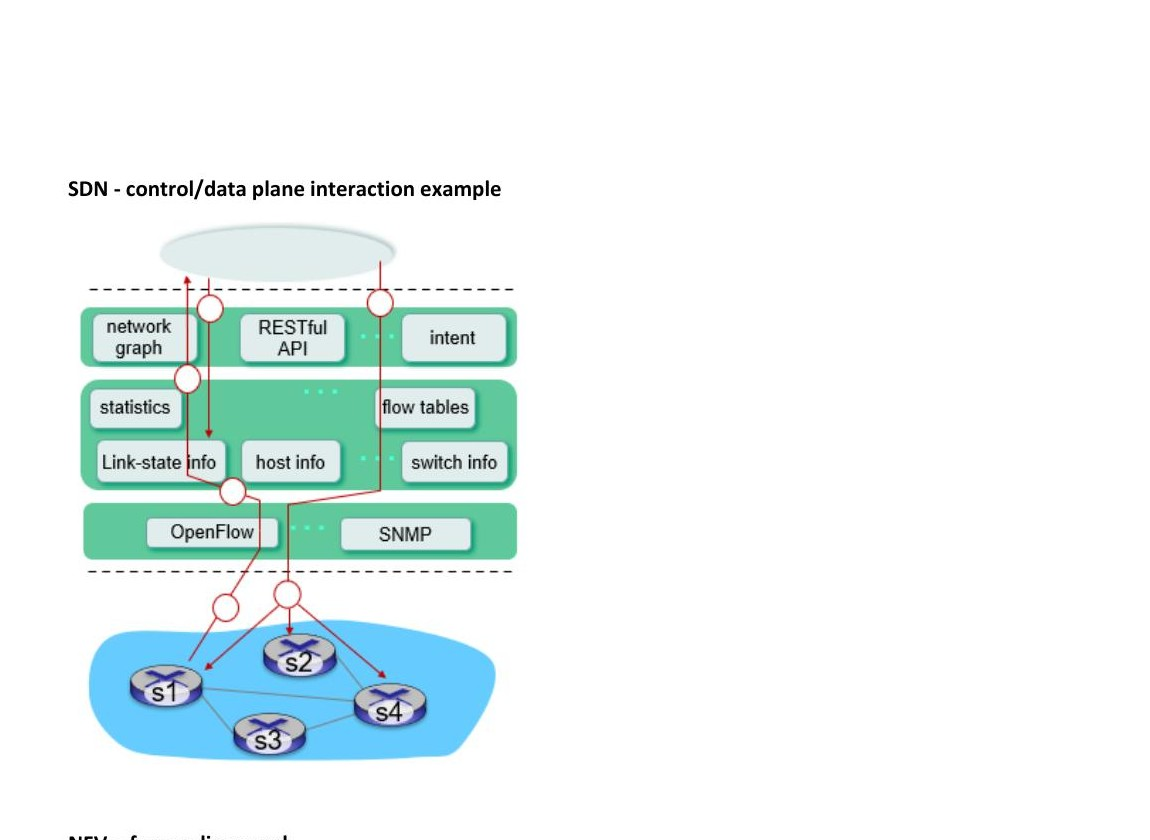
\includegraphics[keepaspectratio]{images/exam-mod2-sdn-control-data-interaction.jpg}}

\subsection{Descrizione dell'immagine}\label{descrizione-dellimmagine-9}

Lo schema è diviso in due parti da una linea tratteggiata. In alto, il
\textbf{Control Plane} (rettangolo bianco) con i componenti: network
graph, RESTful API, intent, statistics, flow tables, Link-state info,
host info, switch info, e due protocolli di southbound:
\textbf{OpenFlow} e \textbf{SNMP}. In basso, il \textbf{Data Plane}
(sfondo azzurro) con quattro switch (s1, s2, s3, s4) interconnessi.

\subsection{Cosa dire all'esame}\label{cosa-dire-allesame-10}

Questo schema mostra come il controller SDN interagisce concretamente
con il data plane, evidenziando le due direzioni di comunicazione:
\textbf{southbound} (controller → switch) e \textbf{northbound} (switch
→ controller).

\textbf{Il controller SDN mantiene internamente:} - \textbf{Network
graph}: un grafo della topologia completo, aggiornato in tempo reale.
Ogni nodo è uno switch o un host, ogni arco è un link con la sua
capacità. - \textbf{Link-state info}: lo stato di ogni link
(attivo/down, latenza, utilizzo) raccolto tramite LLDP o SNMP. -
\textbf{Host info}: la posizione di ogni host nella rete (a quale porta
di quale switch è connesso). - \textbf{Switch info}: le caratteristiche
di ogni switch (numero di porte, OpenFlow version, capabilities). -
\textbf{Statistics}: contatori di pacchetti e byte per ogni flow entry,
per traffic engineering e monitoring. - \textbf{Flow tables}: le regole
di forwarding da installare negli switch.

\textbf{Interfaccia verso le applicazioni (Northbound):} -
\textbf{RESTful API}: le applicazioni di rete (routing, load balancing,
ACL) interrogano e modificano lo stato del controller tramite API REST.
- \textbf{Intent}: alcune implementazioni supportano un livello di
astrazione più alto, dove le applicazioni esprimono ``intenzioni'' (es.
``garantisci 10 Mbps di banda tra h1 e h2'') che il controller traduce
in flow rules.

\textbf{Interfaccia verso gli switch (Southbound):} - \textbf{OpenFlow}:
protocollo principale per installare le flow rule e ricevere packet-in
dagli switch. - \textbf{SNMP} (\emph{Simple Network Management
Protocol}): usato per raccogliere statistiche di gestione dagli switch
(link status, error counters, ecc.) anche da switch non necessariamente
OpenFlow.

\begin{center}\rule{0.5\linewidth}{0.5pt}\end{center}

\section{NFV --- Forwarding Graph}\label{nfv-forwarding-graph}

\pandocbounded{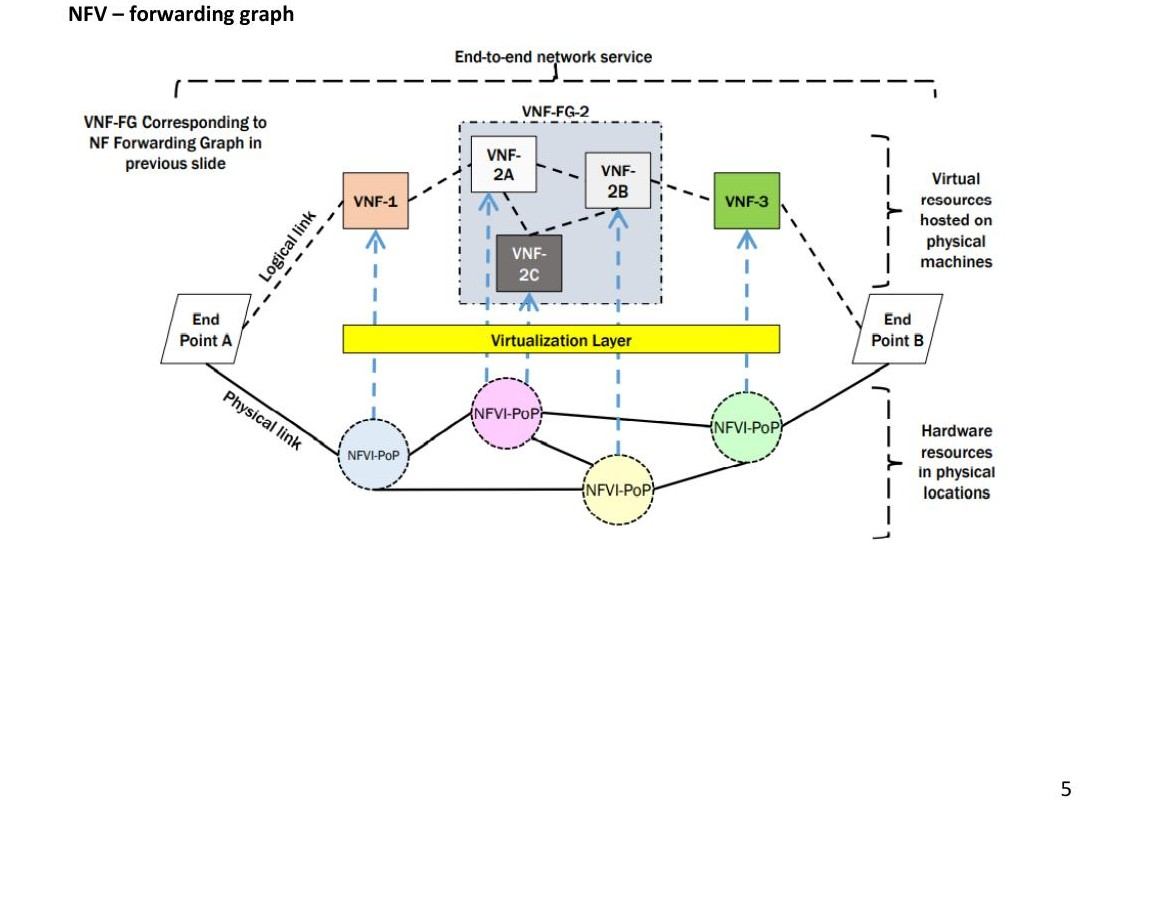
\includegraphics[keepaspectratio]{images/exam-mod2-nfv-forwarding-graph.jpg}}

\subsection{Descrizione
dell'immagine}\label{descrizione-dellimmagine-10}

Lo schema mostra un servizio di rete end-to-end tra \textbf{End Point A}
(a sinistra) e \textbf{End Point B} (a destra). Il servizio è composto
da: \textbf{VNF-1} (in basso a sinistra), il sotto-grafo
\textbf{VNF-FG-2} (nel riquadro centrale, composto da VNF-2A, VNF-2B e
VNF-2C), e \textbf{VNF-3} (in alto a destra). I link logici (frecce
tratteggiate) indicano la catena di forwarding. In basso, tre
\textbf{NFVI-PoP} (punti di presenza dell'infrastruttura NFV) sono
connessi tramite physical links. Una \textbf{Virtualization Layer}
separa il livello logico dal livello fisico.

\subsection{Cosa dire all'esame}\label{cosa-dire-allesame-11}

Questo schema rappresenta il concetto di \textbf{VNF Forwarding Graph}
(VNF-FG), che è il modo in cui NFV formalizza un servizio di rete
end-to-end.

\textbf{L'idea fondamentale di NFV:} invece di implementare funzioni di
rete (firewall, NAT, load balancer, media gateway) in hardware
proprietario dedicato, NFV le implementa come software --- chiamate
\textbf{VNF} (\emph{Virtualized Network Functions}) --- eseguito su
infrastruttura hardware commodity (server COTS). Il decoupling tra
funzione e hardware porta flessibilità, scalabilità e riduzione dei
costi.

\textbf{Il Forwarding Graph:} un servizio di rete non è una singola
funzione, ma una \textbf{composizione di funzioni} applicate in sequenza
al traffico. Il grafo mostra: - Il traffico entra da \textbf{End Point
A}, passa attraverso \textbf{VNF-1}, poi attraverso il sotto-grafo
\textbf{VNF-FG-2} (che a sua volta compone internamente VNF-2A → VNF-2B
e VNF-2C in parallelo), poi attraverso \textbf{VNF-3}, e infine
raggiunge \textbf{End Point B}. - I link logici (tratteggiati)
rappresentano connettività virtuale: due VNF sono logicamente connesse,
ma possono fisicamente trovarsi su macchine diverse.

\textbf{I grafi sono nidificati:} VNF-FG-2 è esso stesso un sotto-grafo
all'interno del grafo principale. Questo consente la riusabilità:
VNF-FG-2 può essere istanziato in altri servizi senza ridefinirlo.

\textbf{L'infrastruttura fisica (NFVI):} le VNF girano su nodi fisici
chiamati \textbf{NFVI-PoP} (\emph{Network Function Virtualization
Infrastructure Point of Presence}). Sono server COTS distribuiti
geograficamente, interconnessi da una rete di trasporto fisica. La
\textbf{Virtualization Layer} (hypervisor o container engine) astrae le
risorse fisiche e consente a più VNF di condividere lo stesso hardware.

\textbf{Il problema del VNF placement:} dato il grafo logico del
servizio, occorre decidere dove deployare fisicamente ogni VNF
nell'infrastruttura. Questo è un problema di ottimizzazione NP-hard che
considera: latenza end-to-end, capacità dei nodi, banda dei link, costi
di deployment, requisiti di QoS per ogni slice di rete.

\begin{center}\rule{0.5\linewidth}{0.5pt}\end{center}

\section{NFV --- Management and
Orchestration}\label{nfv-management-and-orchestration}

\pandocbounded{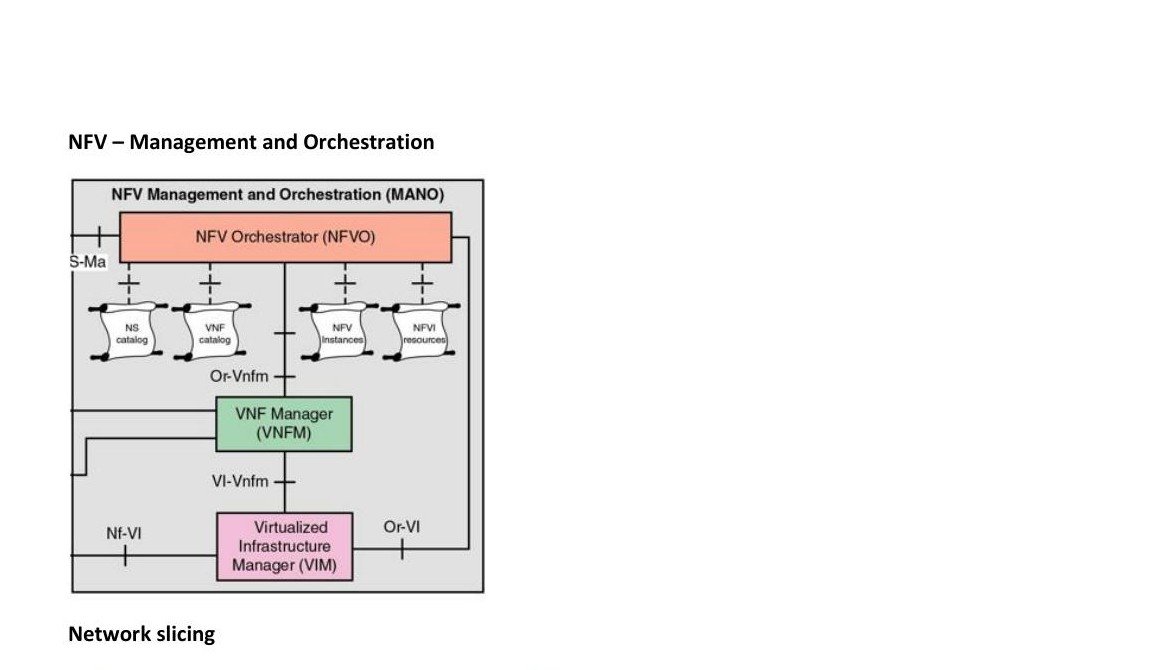
\includegraphics[keepaspectratio]{images/exam-mod2-nfv-mano.jpg}}

\subsection{Descrizione
dell'immagine}\label{descrizione-dellimmagine-11}

Lo schema mostra il framework \textbf{NFV MANO} (\emph{Management and
Orchestration}) secondo ETSI. Al livello superiore c'è il blocco
\textbf{NFV Management and Orchestration (MANO)} che contiene:
l'\textbf{NFV Orchestrator (NFVO)} in cima (con NS catalog e VNF
catalog), connesso tramite l'interfaccia \textbf{Or-Vnfm} al \textbf{VNF
Manager (VNFM)}, che a sua volta è connesso tramite \textbf{VI-Vnfm} al
\textbf{Virtualized Infrastructure Manager (VIM)}. Il VIM è connesso
all'\textbf{NFVI} (l'infrastruttura virtuale) tramite l'interfaccia
\textbf{Nf-Vi} e all'\textbf{Or-Vi} direttamente dall'NFVO.
L'interfaccia \textbf{S-Ma} connette un sistema esterno (OSS/BSS)
all'NFVO.

\subsection{Cosa dire all'esame}\label{cosa-dire-allesame-12}

Questo schema mostra il framework di \textbf{gestione e orchestrazione
NFV} standardizzato da ETSI, che è il ``piano di controllo''
dell'ecosistema NFV.

\textbf{NFV Orchestrator (NFVO):} è il componente di più alto livello.
Ha due responsabilità principali: 1. \textbf{Network services
orchestration}: gestisce il ciclo di vita dei \textbf{Network Service
(NS)} end-to-end, ovvero istanzia, aggiorna e termina l'intero VNF
Forwarding Graph. Può istanziare nuovi VNFM se necessario. 2.
\textbf{Resource orchestration}: gestisce le risorse globali dell'NFVI,
allocandole ai servizi in base alle policy e ai requisiti di QoS. Il
NFVO mantiene due repository: il \textbf{NS Catalog} (template dei
servizi di rete come Network Service Descriptor) e il \textbf{VNF
Catalog} (descrittori di ogni VNF, i VNFD).

\textbf{VNF Manager (VNFM):} gestisce il \textbf{ciclo di vita delle
istanze VNF} singole: - \textbf{Istanziazione}: crea una nuova istanza
VNF su una VM o container nell'NFVI. - \textbf{Scaling}: aumenta o
riduce la capacità di una VNF (scaling out/in orizzontale, scaling
up/down verticale) in base al carico. - \textbf{Healing}: rileva e
gestisce i fault delle VNF (auto-healing o assistito). -
\textbf{Terminazione}: distrugge l'istanza quando non serve più. Il VNFM
comunica con il NFVO tramite \textbf{Or-Vnfm} e con il VIM tramite
\textbf{Vi-Vnfm} (o \textbf{Ve-Vnfm} verso le VNF stesse).

\textbf{Virtualized Infrastructure Manager (VIM):} controlla e gestisce
le risorse fisiche e virtuali dell'NFVI (compute, storage, network).
Piattaforme IaaS come \textbf{OpenStack} fungono da VIM. Il VIM alloca
VM o container alle VNF, configura la rete virtuale (vSwitch, VLAN), e
monitora l'utilizzo delle risorse. Un MANO può orchestrare più VIM
distribuiti geograficamente.

\textbf{Le interfacce di riferimento:} - \textbf{Or-Vi} (NFVO → VIM):
l'orchestratore può richiedere risorse direttamente al VIM. -
\textbf{S-Ma}: collega sistemi OSS/BSS dell'operatore (Operations
Support System / Business Support System) al MANO per l'integrazione con
i sistemi aziendali.

\begin{calloutnote}{Implementazioni open source}

Le principali implementazioni open source del MANO sono \textbf{OSM}
(\emph{Open Source MANO}, promossa da ETSI) e \textbf{ONAP} (\emph{Open
Network Automation Platform}, Linux Foundation). Entrambe sono usate
nelle reti 5G commerciali.

\end{calloutnote}

\begin{center}\rule{0.5\linewidth}{0.5pt}\end{center}

\section{Network Slicing}\label{network-slicing}

\pandocbounded{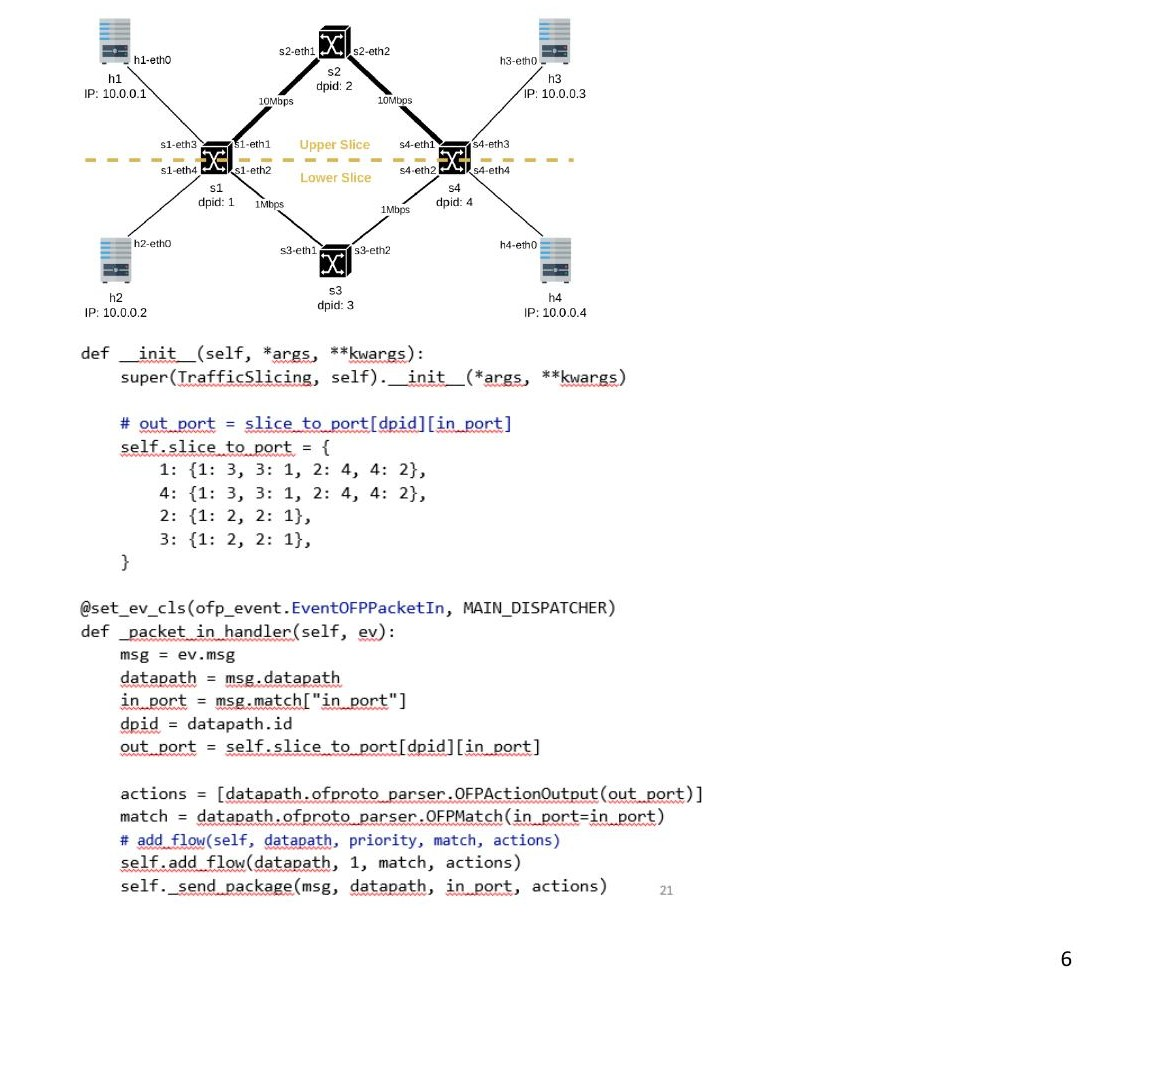
\includegraphics[keepaspectratio]{images/exam-mod2-network-slicing.jpg}}

\subsection{Descrizione
dell'immagine}\label{descrizione-dellimmagine-12}

Lo schema è composto da due parti. In alto, la topologia di rete:
quattro switch (s1 dpid:1, s2 dpid:2, s3 dpid:3, s4 dpid:4)
interconnessi, con quattro host (h1 IP:10.0.0.1, h2 IP:10.0.0.2, h3
IP:10.0.0.3, h4 IP:10.0.0.4). Una linea tratteggiata superiore indica
l'\textbf{Upper Slice} (che attraversa s1-eth1 → s4-eth1), e una linea
tratteggiata inferiore indica la \textbf{Lower Slice} (che attraversa
s1-eth2 → s4-eth2). S2 ha capacità 10 Mbps, s1 e s4 hanno 1 Mbps. In
basso, codice Python che implementa il controller Ryu per lo slicing,
con un dizionario \texttt{slice\_to\_port} che mappa (dpid, in\_port) →
out\_port.

\subsection{Cosa dire all'esame}\label{cosa-dire-allesame-13}

Questo schema mostra l'implementazione pratica del \textbf{Network
Slicing} tramite SDN con il controller \textbf{Ryu} (scritto in Python),
uno dei casi d'uso più importanti di SDN e NFV nel contesto del 5G.

\textbf{Cosa è il Network Slicing:} la possibilità di creare su una
stessa infrastruttura fisica \textbf{reti logicamente separate}
(\emph{slice}), ciascuna con le proprie caratteristiche di QoS, banda,
latenza e isolamento. In questo esempio, sulla stessa topologia fisica
(s1-s2-s4 e s1-s3-s4) vengono create due slice indipendenti: -
\textbf{Upper Slice}: usa il percorso s1(eth1) → s2 → s4(eth1), con
capacità 10 Mbps (il link via s2 ha banda più alta). - \textbf{Lower
Slice}: usa il percorso s1(eth2) → s3 → s4(eth2), con capacità 1 Mbps.

\textbf{Il codice Python --- TrafficSlicing:} il dizionario
\texttt{slice\_to\_port} è il cuore dell'implementazione. Per ogni
switch (dpid) e per ogni porta di ingresso (in\_port), specifica la
porta di uscita:

\begin{Shaded}
\begin{Highlighting}[]
\VariableTok{self}\NormalTok{.slice\_to\_port }\OperatorTok{=}\NormalTok{ \{}
    \DecValTok{1}\NormalTok{: \{}\DecValTok{1}\NormalTok{: }\DecValTok{3}\NormalTok{, }\DecValTok{3}\NormalTok{: }\DecValTok{1}\NormalTok{, }\DecValTok{2}\NormalTok{: }\DecValTok{4}\NormalTok{, }\DecValTok{4}\NormalTok{: }\DecValTok{2}\NormalTok{\},  }\CommentTok{\# switch s1 (dpid=1)}
    \DecValTok{4}\NormalTok{: \{}\DecValTok{1}\NormalTok{: }\DecValTok{3}\NormalTok{, }\DecValTok{3}\NormalTok{: }\DecValTok{1}\NormalTok{, }\DecValTok{2}\NormalTok{: }\DecValTok{4}\NormalTok{, }\DecValTok{4}\NormalTok{: }\DecValTok{2}\NormalTok{\},  }\CommentTok{\# switch s4 (dpid=4)}
    \DecValTok{2}\NormalTok{: \{}\DecValTok{1}\NormalTok{: }\DecValTok{2}\NormalTok{, }\DecValTok{2}\NormalTok{: }\DecValTok{1}\NormalTok{\},               }\CommentTok{\# switch s2 (dpid=2)}
    \DecValTok{3}\NormalTok{: \{}\DecValTok{1}\NormalTok{: }\DecValTok{2}\NormalTok{, }\DecValTok{2}\NormalTok{: }\DecValTok{1}\NormalTok{\},               }\CommentTok{\# switch s3 (dpid=3)}
\NormalTok{\}}
\end{Highlighting}
\end{Shaded}

Il gestore \texttt{\_packet\_in\_handler} è chiamato dal controller Ryu
ogni volta che uno switch riceve un pacchetto che non ha una flow entry
corrispondente (\emph{packet-in}). Il controller legge il dpid dello
switch e la porta di ingresso, cerca nel dizionario la porta di uscita,
installa una \textbf{flow rule} nello switch (con
\texttt{self.add\_flow(datapath,\ 1,\ match,\ actions)}) e forwarda il
pacchetto.

\textbf{Il ruolo di SDN nel Network Slicing:} senza SDN, separare il
traffico richiederebbe VLAN, configurazione manuale di ogni switch, o
hardware dedicato per ogni slice. Con SDN, è sufficiente un controller
centralizzato che installa le regole di forwarding appropriate per ogni
flusso, realizzando lo slicing in software.

\begin{callouttip}{Rilevanza nel 5G}

Il Network Slicing è uno dei pilastri del 5G: slice diverse possono
essere dedicate a eMBB (enhanced Mobile Broadband, alta banda), URLLC
(Ultra-Reliable Low-Latency Communications, bassa latenza per
applicazioni critiche) e mMTC (massive Machine Type Communications, IoT
a bassa potenza). La separazione logica garantisce che i requisiti di
QoS di una slice non vengano degradati dalle altre.

\end{callouttip}

\begin{center}\rule{0.5\linewidth}{0.5pt}\end{center}

\section{Fourier Series (Serie di
Fourier)}\label{fourier-series-serie-di-fourier}

\pandocbounded{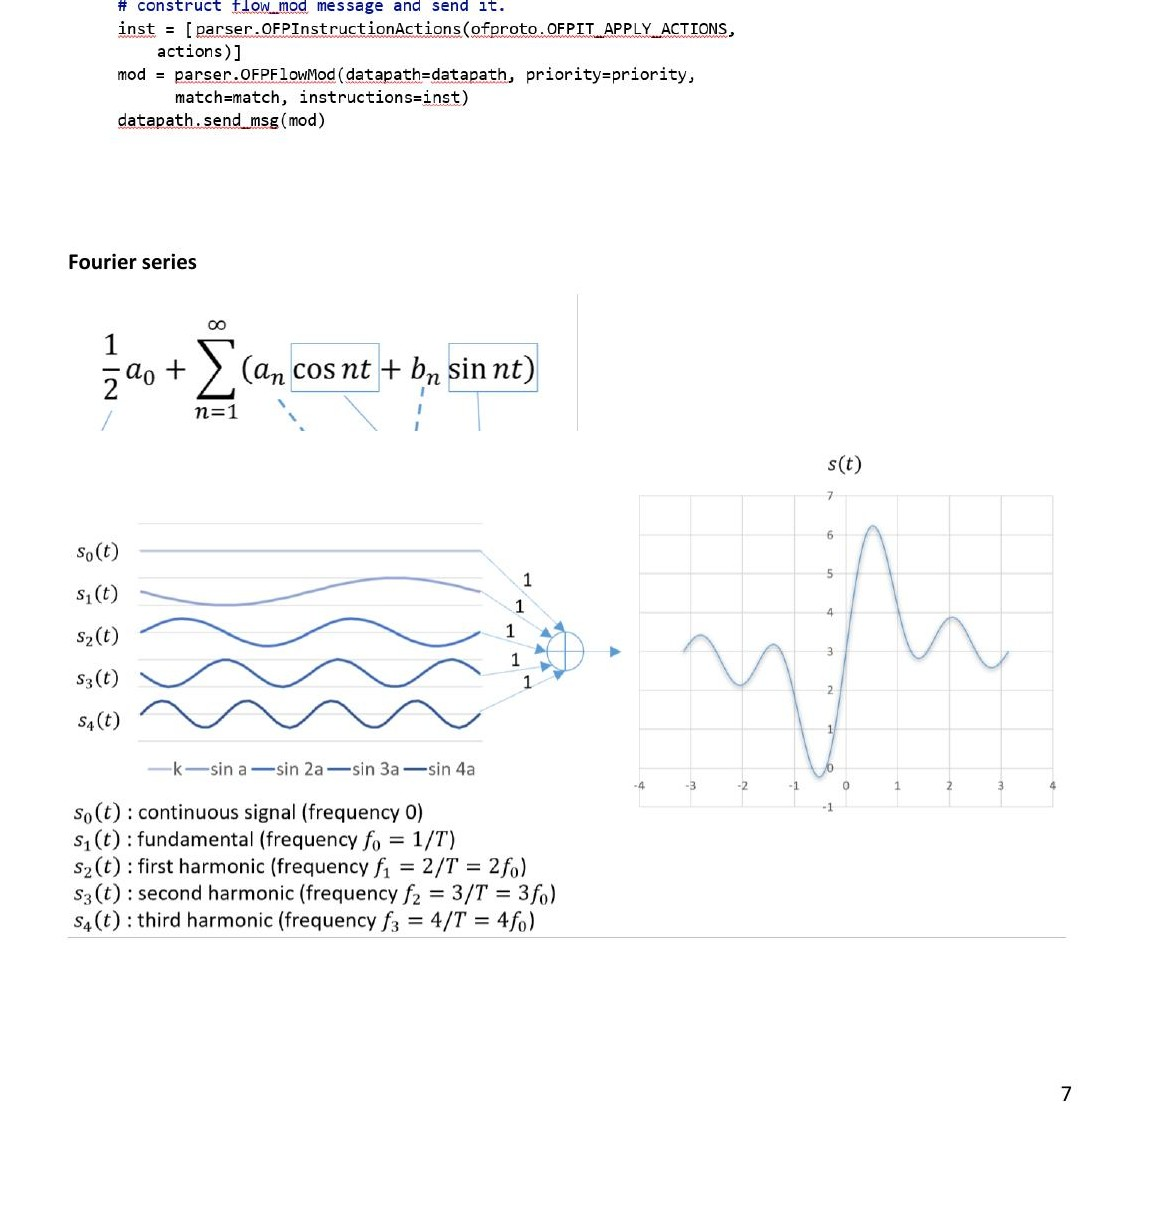
\includegraphics[keepaspectratio]{images/exam-mod2-fourier-series.jpg}}

\subsection{Descrizione
dell'immagine}\label{descrizione-dellimmagine-13}

Lo schema mostra: in alto a sinistra, la formula matematica della serie
di Fourier
\(\frac{1}{2}a_0 + \sum_{n=1}^{\infty}(a_n \cos nt + b_n \sin nt)\) con
i termini \(a_n \cos nt\) e \(b_n \sin nt\) evidenziati. A sinistra,
cinque segnali sovrapposti: \(s_0(t)\) (segnale continuo, linea piatta),
\(s_1(t)\) (fondamentale, ampiezza 1), \(s_2(t)\) (prima armonica,
ampiezza 1), \(s_3(t)\) (seconda armonica, ampiezza 1), \(s_4(t)\)
(terza armonica, ampiezza 1), con la legenda ``--k --sin a --sin 2a
--sin 3a --sin 4a''. A destra, il segnale \(s(t)\) risultante dalla loro
somma, che mostra una forma d'onda composta.

\subsection{Cosa dire all'esame}\label{cosa-dire-allesame-14}

Questo schema illustra il concetto fondamentale della \textbf{Serie di
Fourier}: qualsiasi segnale periodico può essere decomposto in una somma
(infinita) di funzioni sinusoidali a frequenze multiple della frequenza
fondamentale.

\textbf{La formula:}
\[s(t) = \frac{1}{2}a_0 + \sum_{n=1}^{\infty}\left(a_n \cos(nt) + b_n \sin(nt)\right)\]

dove i coefficienti si calcolano come:
\[a_0 = \frac{1}{\pi}\int_{-\pi}^{\pi} s(t)\,dt \qquad a_n = \frac{1}{\pi}\int_{-\pi}^{\pi} s(t)\cos(nt)\,dt \qquad b_n = \frac{1}{\pi}\int_{-\pi}^{\pi} s(t)\sin(nt)\,dt\]

\textbf{Interpretazione fisica:} ogni segnale periodico è la ``somma di
sinusoidi''. Il termine \(\frac{1}{2}a_0\) è la \textbf{componente
continua} (il valor medio del segnale, \(s_0\) nel diagramma). I termini
successivi sono le \textbf{armoniche}: \(s_1\) è la
\textbf{fondamentale} con frequenza \(f_0 = 1/T\), \(s_2\) è la
\textbf{prima armonica} con frequenza \(f_1 = 2/T = 2f_0\), \(s_3\) la
seconda armonica a \(3f_0\), \(s_4\) la terza armonica a \(4f_0\), e
così via.

\textbf{Il significato pratico per le reti:} il canale trasmissivo non
tratta tutte le frequenze allo stesso modo: alcune le attenua più di
altre. Sapere quali frequenze compongono un segnale --- cioè conoscere
il suo \textbf{spettro} --- permette di: - Predire come il segnale si
deformerà attraverso il canale. - Dimensionare la \textbf{banda}
necessaria (quante armoniche servono per rappresentare il segnale
fedelmente). - Progettare filtri per rimuovere componenti indesiderate.

\textbf{Le condizioni di Dirichlet} garantiscono l'esistenza della
serie: è sufficiente che il segnale sia \emph{piecewise continuous}
(composto da un numero finito di pezzi continui con limite finito nei
punti di discontinuità). In corrispondenza delle discontinuità la serie
converge alla media dei limiti sinistro e destro.

\begin{calloutwarning}{Fenomeno di Gibbs}

Quando la serie di Fourier approssima un segnale con discontinuità (es.
onda quadra), si osserva un \emph{overshoot} del ≈9\% dell'ampiezza del
salto che non scompare mai, per quanto si aumenti il numero di
armoniche. Le oscillazioni nel tratto piatto si riducono, ma il picco al
salto rimane costante.

\end{calloutwarning}

\begin{center}\rule{0.5\linewidth}{0.5pt}\end{center}

\section{DFT (Discrete Fourier
Transform)}\label{dft-discrete-fourier-transform}

\subsection{Descrizione
dell'immagine}\label{descrizione-dellimmagine-14}

Lo schema mostra la formula della \textbf{DFT} (\emph{Discrete Fourier
Transform}):
\[S_f = \sum_{n=0}^{N-1} s_n \, e^{-j\frac{2\pi f}{N}n} \quad \text{with } f = 0, 1, \ldots, N-1\]

\subsection{Cosa dire all'esame}\label{cosa-dire-allesame-15}

La \textbf{Trasformata di Fourier Discreta} (DFT) è la versione
\emph{calcolabile da un computer} dell'analisi di Fourier: opera su un
segnale discreto di lunghezza finita \(N\) e produce \(N\) coefficienti
frequenziali.

\textbf{La formula:} dato un segnale campionato \(s_n\) (con
\(n = 0, 1, \ldots, N-1\)), la DFT calcola il coefficiente \(S_f\) per
ogni frequenza discreta \(f = 0, 1, \ldots, N-1\):
\[S_f = \sum_{n=0}^{N-1} s_n \, e^{-j\frac{2\pi f}{N}n}\]

\textbf{Interpretazione:} - Ogni coefficiente \(S_f\) è un numero
complesso: il suo \textbf{modulo} \(|S_f|\) è l'ampiezza del contributo
alla frequenza \(f\), la sua \textbf{fase} \(\arg(S_f)\) è lo sfasamento
della componente sinusoidale corrispondente. - Le frequenze reali
rappresentate sono \(f_k = k \cdot \frac{f_c}{N}\), dove \(f_c\) è la
frequenza di campionamento.

\textbf{Relazione con la Serie di Fourier:} la DFT è il corrispettivo
discreto della serie di Fourier: la serie opera su segnali periodici
continui e produce coefficienti \(S_n\), la DFT opera su sequenze finite
discrete e produce \(N\) coefficienti \(S_f\). La DFT assume
implicitamente che il segnale di \(N\) campioni sia la ripetizione
periodica di un pattern.

\textbf{L'algoritmo FFT:} il calcolo diretto della DFT ha complessità
\(O(N^2)\) (ogni \(S_f\) richiede \(N\) moltiplicazioni e addizioni
complesse). L'algoritmo \textbf{FFT} (\emph{Fast Fourier Transform}),
sviluppato da Cooley e Tukey nel 1965, riduce la complessità a
\(O(N \log N)\) sfruttando la simmetria del fattore
\(e^{-j\frac{2\pi f}{N}n}\). Per \(N = 1024\) punti, la FFT è ≈100 volte
più veloce della DFT diretta.

\textbf{Applicazioni pratiche:} - \textbf{Analisi spettrale} di segnali
acquisiti (ECG, audio, sismici). - \textbf{OFDM} (\emph{Orthogonal
Frequency Division Multiplexing}): il segnale 4G/5G è creato con una
IFFT e demodulato con una FFT, permettendo di trasmettere dati su
migliaia di sottoportanti ortogonali simultaneamente. - Filtraggio
digitale e compressione (JPEG usa la DCT, variante della DFT).

\begin{center}\rule{0.5\linewidth}{0.5pt}\end{center}

\section{Sampling and Aliasing (Campionamento e
Aliasing)}\label{sampling-and-aliasing-campionamento-e-aliasing}

\pandocbounded{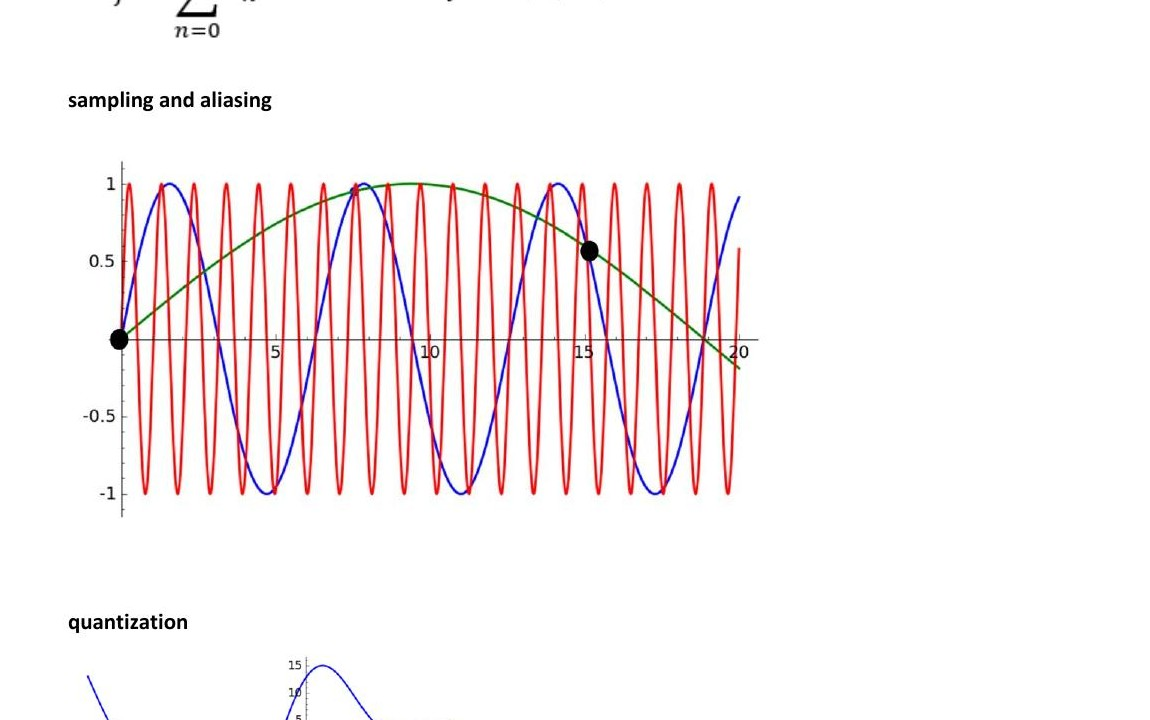
\includegraphics[keepaspectratio]{images/exam-mod2-sampling-aliasing.jpg}}

\subsection{Descrizione
dell'immagine}\label{descrizione-dellimmagine-15}

Lo schema mostra un grafico con tre segnali sovrapposti nell'asse tempo
(da 0 a 20) e ampiezza (da -1 a 1). Il segnale \textbf{rosso} è ad alta
frequenza (molti cicli nel grafico). Il segnale \textbf{blu} è a bassa
frequenza (pochi cicli). Il segnale \textbf{verde} è un'involucro che
segna lentamente. Due \textbf{punti neri} evidenziano due istanti di
campionamento: in quei punti, segnale rosso e segnale blu hanno
\textbf{esattamente lo stesso valore}. I punti neri sono al valore ≈0.5
a t≈0 e a t≈15.

\subsection{Cosa dire all'esame}\label{cosa-dire-allesame-16}

Questo schema illustra il \textbf{problema dell'aliasing}, uno dei
fenomeni più importanti nella teoria del campionamento digitale.

\textbf{Il campionamento:} convertire un segnale analogico continuo in
una sequenza discreta \(s_n = s(nT_c)\) significa prelevare il valore
del segnale a intervalli regolari di periodo \(T_c = 1/f_c\) (frequenza
di campionamento). Ma campionare introduce un'ambiguità: da un insieme
finito di campioni non si può distinguere univocamente quale segnale li
ha generati.

\textbf{L'aliasing:} il segnale rosso (alta frequenza \(f_h\)) e il
segnale blu (bassa frequenza \(f_l\)) producono \textbf{identici
campioni} (i punti neri). Se si guardano solo i campioni, è impossibile
capire se il segnale originale era quello rosso o quello blu. Il segnale
a bassa frequenza è l'\textbf{alias} di quello ad alta frequenza:
un'identità fantasma creata dal sottocampionamento.

\textbf{Il Teorema di Nyquist-Shannon:} affinché un segnale di banda
\(B\) (frequenza massima \(f_{max}\)) sia ricostruito perfettamente dai
suoi campioni, la frequenza di campionamento deve soddisfare:
\[f_c \geq 2 \cdot f_{max}\]

La frequenza \(f_{Nyquist} = f_c/2\) è la massima frequenza
rappresentabile senza aliasing. Se nel segnale originale sono presenti
frequenze superiori a \(f_{Nyquist}\), queste appaiono come frequenze
più basse nello spettro discreto --- l'aliasing appunto.

\textbf{Come prevenire l'aliasing:} si applica un \textbf{filtro
anti-aliasing} (filtro passa-basso analogico) prima del campionatore,
che elimina tutte le componenti con \(f > f_c/2\). Solo dopo si
campiona. Questo garantisce che il segnale digitale rappresenti
fedelmente l'originale entro la banda di interesse.

\textbf{Applicazioni:} - Audio CD: frequenza di campionamento 44.1 kHz →
rappresenta fedelmente frequenze fino a 22.05 kHz (limite dell'udito
umano ≈20 kHz). - Telefonia: 8 kHz (voce fino a 4 kHz). - WiFi e reti
cellulari: i ricevitori devono campionare il segnale RF ad almeno
\(2 \times B_{canale}\).

\begin{center}\rule{0.5\linewidth}{0.5pt}\end{center}

\section{Quantization
(Quantizzazione)}\label{quantization-quantizzazione}

\pandocbounded{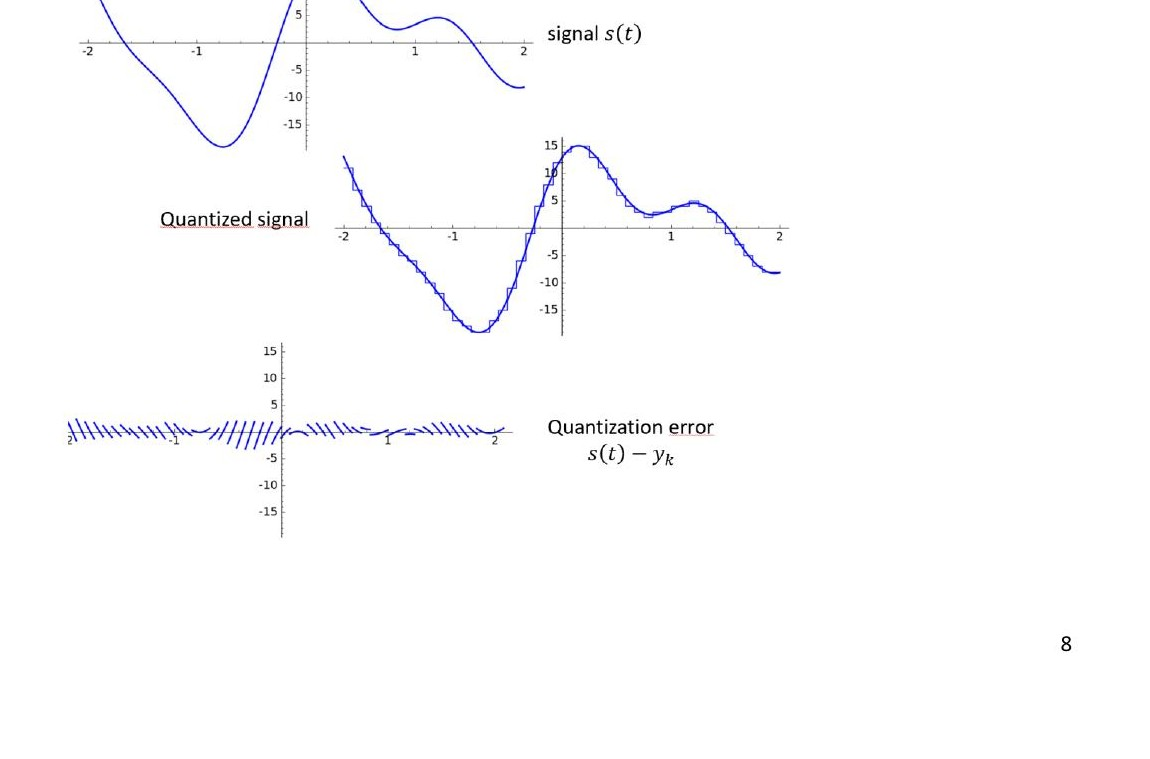
\includegraphics[keepaspectratio]{images/exam-mod2-quantization.jpg}}

\subsection{Descrizione
dell'immagine}\label{descrizione-dellimmagine-16}

Lo schema mostra tre grafici verticalmente sovrapposti, tutti con asse x
da -2 a 2 e asse y da -15 a 15. Il grafico superiore mostra il
\textbf{segnale analogico \(s(t)\)} continuo e fluido. Il grafico
centrale mostra il \textbf{segnale quantizzato} come approssimazione a
gradini del segnale originale (ogni campione viene arrotondato al
livello discreto più vicino). Il grafico inferiore mostra
l'\textbf{errore di quantizzazione} \(s(t) - y_k\): la differenza tra
segnale originale e quantizzato, che appare come un segnale oscillante
ad alta frequenza di piccola ampiezza.

\subsection{Cosa dire all'esame}\label{cosa-dire-allesame-17}

Questo schema illustra la \textbf{quantizzazione}, il secondo passo
nella conversione analogico-digitale (il primo è il campionamento). Dopo
aver campionato il segnale nel tempo, ogni campione deve essere
rappresentato con un numero finito di bit, cioè deve essere approssimato
al livello discreto più vicino tra un insieme finito di valori
possibili.

\textbf{Il processo:} dato un campione \(s(nT_c)\) con valore reale, si
sceglie il \textbf{livello di quantizzazione} \(y_k\) più vicino e si
assegna il codice binario corrispondente. Se si usano \(M\) bit per
campione, si hanno \(2^M\) livelli di quantizzazione, spaziati di un
passo \(\Delta = \frac{s_{max} - s_{min}}{2^M}\).

\textbf{L'errore di quantizzazione:} l'approssimazione introduce un
errore \(e = s(t) - y_k\), che ha valore assoluto al massimo
\(\Delta/2\). Questo errore è inevitabile: è il prezzo del passaggio dal
continuo al discreto. Nel grafico in basso si vede chiaramente: l'errore
è un segnale oscillante (dovuto all'arrotondamento al gradino) con
ampiezza piccola (≈\(\Delta/2\)) e frequenza elevata.

\textbf{Trade-off:} - Aumentare \(M\) (più bit per campione) riduce
\(\Delta\) e quindi l'errore di quantizzazione, ma aumenta il
\textbf{bitrate} richiesto: \(\text{Bitrate} = f_c \times M\) bit/s. -
Il \textbf{SNR di quantizzazione} cresce approssimativamente di 6 dB per
ogni bit aggiunto: \(\text{SNR}_{dB} \approx 6.02 \cdot M + 1.76\) dB.

\textbf{Applicazioni:} - \textbf{Audio CD}: 16 bit per campione → 96 dB
di range dinamico (65536 livelli). - \textbf{Telefonia}: 8 bit
(companding μ-law/A-law) → 256 livelli, ma compressione logaritmica per
migliorare la qualità percepita a basse ampiezze. - \textbf{Sensori
IoT}: 12 bit ADC tipici per temperatura, pressione, accelerometro.

\begin{calloutnote}{Errore di quantizzazione come rumore}

Nell'analisi statistica, l'errore di quantizzazione viene modellato come
\textbf{rumore bianco} uniforme nell'intervallo
\([-\Delta/2, +\Delta/2]\) quando il segnale è molto più grande di
\(\Delta\) (assunzione di piccolo passo di quantizzazione). Questo
consente di applicare la teoria del rumore per dimensionare il sistema:
il SNR post-quantizzazione deve superare una soglia minima per garantire
la qualità del servizio.

\end{calloutnote}

\begin{calloutnote}{Sintesi — Pipeline di digitalizzazione}

Il percorso completo dalla sorgente analogica al digitale è: 1.
\textbf{Filtraggio anti-aliasing} (passa-basso, \(f_{taglio} = f_c/2\))
→ elimina le frequenze che causerebbero aliasing. 2.
\textbf{Campionamento} a \(f_c \geq 2 f_{max}\) → sequenza discreta nel
tempo. 3. \textbf{Quantizzazione} con \(M\) bit → sequenza digitale. 4.
\textbf{Codifica} binaria → bitstream trasmissibile. Il bitrate
risultante è \(f_c \times M\) bit/s, e deve rientrare nella capacità del
canale \(C = B \log_2(1 + \text{SNR})\) per garantire la trasmissione
senza errori.

\end{calloutnote}

\newpage

\backmatter
\end{document}
